% Meta-Informationen -------------------------------------------------------
%		Informationen �ber das Dokument, wie z.B. Titel, Autor, Matrikelnr. etc
%		werden in der Datei _Meta.tex definiert und k�nnen danach global
%		verwendet werden.
% --------------------------------------------------------------------------
% Informationen ------------------------------------------------------------
% 	Definition von globalen Parametern, die im gesamten Dokument verwendet
% 	werden k�nnen (z.B auf dem Deckblatt etc.).
% --------------------------------------------------------------------------
\newcommand{\titel}{Untersuchung zur Eignung von Graphdatenbanksystemen f�r die Analyse von Informationsnetzwerken}
\newcommand{\art}{Masterarbeit}
\newcommand{\ort}{Leipzig}
\newcommand{\hochschule}{Universit�t Leipzig}
\newcommand{\fachgebiet}{Abteilung Datenbanken}
\newcommand{\fakultaet}{Fakult�t f�r Mathematik und Informatik}
\newcommand{\institut}{Institut f�r Informatik}
\newcommand{\autor}{Martin Junghanns}
\newcommand{\matrikelnr}{2780511}
\newcommand{\erstgutachter}{Prof. Dr. Erhard Rahm}
\newcommand{\zweitgutachter}{Dipl.--Ing. Andr� Petermann}
\newcommand{\jahr}{2013}
\newcommand{\invnr}{1337}
\newcommand{\eingereicht}{}

% Eigene Befehle
\newcommand{\todo}[1]{\textbf{\textsc{\textcolor{red}{(TODO: #1)}}}}

% Autorennamen in small caps
\newcommand{\AutorZ}[1]{\textsc{#1}}
\newcommand{\Autor}[1]{\AutorZ{\citeauthor{#1}}}

% Befehle zur semantischen Auszeichnung von Text
\newcommand{\NeuerBegriff}[1]{\textbf{#1}}
\newcommand{\Fachbegriff}[1]{\textit{#1}}
\newcommand{\Prozess}[1]{\textit{#1}}
\newcommand{\Webservice}[1]{\textit{#1}}
\newcommand{\Eingabe}[1]{\texttt{#1}}
\newcommand{\Code}[1]{\texttt{#1}}
\newcommand{\Datei}[1]{\texttt{#1}}
\newcommand{\Datentyp}[1]{\textsf{#1}}
\newcommand{\XMLElement}[1]{\textsf{#1}}

% Abk�rzungen
\newcommand{\vgl}{Vgl.\ }
\newcommand{\ua}{\mbox{u.\,a.\ }}
\newcommand{\zB}{\mbox{z.\,B.\ }}
\newcommand{\bs}{$\backslash$}

% Einfache Anf�hrungszeichen in texttt
\newcommand{\sq}{\textquotesingle}




% Dokumentenkopf -----------------------------------------------------------
% 	Diese Vorlage basiert auf "scrreprt" aus dem koma-script.
%		Die Option draft sollte beim fertigen Dokument ausgeschaltet werden.
% --------------------------------------------------------------------------
\documentclass[
	12pt,						% Schriftgr��e
	DIV10,
	ngerman,					% f�r Umlaute, Silbentrennung etc.
	a4paper,					% Papierformat
	oneside,					% einseitiges Dokument
	titlepage,				% es wird eine Titelseite verwendet
	halfparskip,			% Abstand zwischen Abs�tzen (halbe Zeile)
	normalheadings,		% Gr��e der �berschriften verkleinern
	liststotoc,				% Verzeichnisse im Inhaltsverzeichnis auff�hren
	bibtotoc,				% Literaturverzeichnis im Inhaltsverzeichnis auff�hren
	idxtotoc,				% Index im Inhaltsverzeichnis auff�hren
	tablecaptionabove,	% Beschriftung von Tabellen oberhalb ausgeben
	final						% Status des Dokuments (final/draft)
]{scrreprt}

\renewcommand*\chapterheadstartvskip{\vspace*{-1.5cm}}

% Bentigte Packages -------------------------------------------------------
%		Weitere Packages, die ben�tigt werden, sind in die Datei Packages.tex
%		"ausgelagert", um die Vorlage m�glichst �bersichtlich zu halten.
% --------------------------------------------------------------------------
% Anpassung des Seitenlayouts ----------------------------------------------
% 	siehe Seitenstil.tex
% --------------------------------------------------------------------------
\usepackage[
	automark,			% Kapitelangaben in Kopfzeile automatisch erstellen
	headsepline,	% Trennlinie unter Kopfzeile
	ilines				% Trennlinie linksb�ndig ausrichten
]{scrpage2}

\usepackage{pseudocode}
\usepackage{nicefrac}

% F�r eine sch�ne Anordnung von Bildern
\usepackage{subfigure}

\usepackage{dsfont}
%\usepackage{color}
%
%% Define user colors using the RGB model
%\definecolor{yellow}{rgb}{0.0,1.0,0.0}
%\definecolor{rot}{rgb}{1.0,0.0,0.0}

% Anpassung an Landessprache -----------------------------------------------
% 	Verwendet globale Option german siehe \documentclass
% --------------------------------------------------------------------------
\usepackage[ngerman]{babel}

% Umlaute ------------------------------------------------------------------
% 		Umlaute/Sonderzeichen wie ���� direkt im Quelltext verwenden (CodePage).
%		Erlaubt automatische Trennung von Worten mit Umlauten.
% --------------------------------------------------------------------------
\usepackage[latin1]{inputenc}
\usepackage[T1]{fontenc}
%\usepackage{ae} % "sch�neres" �
\usepackage{textcomp} % Euro-Zeichen etc.
\usepackage{lmodern} % sch���n

% Grafiken -----------------------------------------------------------------
% 		Einbinden von Grafiken [draft oder final]
% 		Option [draft] bindet Bilder nicht ein - auch globale Option
% --------------------------------------------------------------------------
\usepackage[dvips,final]{graphicx}
\usepackage{wrapfig}
\graphicspath{{Bilder/}} % Dort liegen die Bilder des Dokuments

% Befehle aus AMSTeX f�r mathematische Symbole z.B. \boldsymbol \mathbb ----
\usepackage{amsmath,amsfonts,amsthm}

% F�r Index-Ausgabe; \printindex -------------------------------------------
\usepackage{makeidx}

% Einfache Definition der Zeilenabst�nde und Seitenr�nder etc. -------------
\usepackage{setspace}
\usepackage{geometry}

% f�r gedrehte Tabellen
\usepackage{rotating} 

% Symbolverzeichnis --------------------------------------------------------
% 	Symbolverzeichnisse bequem erstellen, beruht auf MakeIndex.
% 		makeindex.exe %Name%.nlo -s nomencl.ist -o %Name%.nls
% 	erzeugt dann das Verzeichnis. Dieser Befehl kann z.B. im TeXnicCenter
%		als Postprozessor eingetragen werden, damit er nicht st�ndig manuell
%		ausgef�hrt werden muss.
%		Die Definitionen sind ausgegliedert in die Datei Abkuerzungen.tex.
% --------------------------------------------------------------------------
\usepackage[intoc]{nomencl}
  \let\abbrev\nomenclature
  \renewcommand{\nomname}{Abk�rzungsverzeichnis}
  \setlength{\nomlabelwidth}{.25\hsize}
  \renewcommand{\nomlabel}[1]{#1 \dotfill}
  \setlength{\nomitemsep}{-\parsep}

% Zum Umflie�en von Bildern -------------------------------------------------
\usepackage{floatflt}

% Zum Einbinden von Programmcode --------------------------------------------
\usepackage{listings}
\usepackage{xcolor} 
\definecolor{hellgelb}{rgb}{1,1,0.9}
\definecolor{colKeys}{rgb}{0,0,1}
\definecolor{colIdentifier}{rgb}{0,0,0}
\definecolor{colComments}{rgb}{1,0,0}
\definecolor{colString}{rgb}{0,0.5,0}
\lstset{%
    float=hbp,%
    basicstyle=\texttt\small, %
    identifierstyle=\color{colIdentifier}, %
    keywordstyle=\color{colKeys}, %
    stringstyle=\color{colString}, %
    commentstyle=\color{colComments}, %
    columns=flexible, %
    tabsize=2, %
    frame=single, %
    extendedchars=true, %
    showspaces=false, %
    showstringspaces=false, %
    numbers=left, %
    numberstyle=\tiny, %
    breaklines=true, %
    backgroundcolor=\color{hellgelb}, %
    breakautoindent=true, %
%    captionpos=b%
}

% Lange URLs umbrechen etc. -------------------------------------------------
\usepackage{url}


%% Wichtig f�r korrekte Zitierweise ------------------------------------------

%\usepackage[square]{natbib}
%% Quellenangaben in eckige Klammern fassen ----------------------------------
%\bibpunct{[}{]}{;}{a}{}{,~}

%% BA-Quellenstyle -----------------------------------------------------------

%\usepackage{babelbib}
%\bibliographystyle{geralpha}

% erm�glicht Zeilenumbr�che in Captions
\usepackage{caption}


% PDF-Optionen --------------------------------------------------------------
\usepackage[
bookmarks,
bookmarksopen=true,
pdftitle={\titel},
pdfauthor={\autor},
pdfcreator={\autor},
pdfsubject={\titel},
pdfkeywords={\titel},
colorlinks=true,
%linkcolor=red, % einfache interne Verkn�pfungen
%anchorcolor=black,% Ankertext
%citecolor=blue, % Verweise auf Literaturverzeichniseintr�ge im Text
%filecolor=magenta, % Verkn�pfungen, die lokale Dateien �ffnen
%menucolor=red, % Acrobat-Men�punkte
%urlcolor=cyan, 
% f�r die Druckversion k�nnen die Farben ausgeschaltet werden:
linkcolor=black, % einfache interne Verkn�pfungen
anchorcolor=black,% Ankertext
citecolor=black, % Verweise auf Literaturverzeichniseintr�ge im Text5
filecolor=black, % Verkn�pfungen, die lokale Dateien �ffnen
menucolor=black, % Acrobat-Men�punkte
urlcolor=black, 
%backref,
%pagebackref,
plainpages=false,% zur korrekten Erstellung der Bookmarks
pdfpagelabels,% zur korrekten Erstellung der Bookmarks
hypertexnames=false,% zur korrekten Erstellung der Bookmarks
linktocpage % Seitenzahlen anstatt Text im Inhaltsverzeichnis verlinken
]{hyperref}

% Zum fortlaufenden Durchnummerieren der Fu�noten ---------------------------
\usepackage{chngcntr}


% f�r lange Tabellen
\usepackage{longtable}
\usepackage{array}
\usepackage{ragged2e}
\usepackage{lscape}

\usepackage{supertabular}

% Spaltendefinition rechtsb�ndig mit definierter Breite ---------------------
\newcolumntype{w}[1]{>{\raggedleft\hspace{0pt}}p{#1}}

% Formatierung von Listen �ndern
\usepackage{paralist}
% Standardeinstellungen:
% \setdefaultleftmargin{2.5em}{2.2em}{1.87em}{1.7em}{1em}{1em}

\usepackage{tablefootnote}
% f�r Ausblenden der Seitenzahl
\usepackage{lipsum}

% Erstellung eines Index und Abk�rzungsverzeichnisses aktivieren -----------
\makeindex
% makeindex Masterarbeit.nlo -s nomencl.ist -o Masterarbeit.nls
\makenomenclature


% Kopf- und Fu�zeilen, Seitenr�nder etc. -----------------------------------
% Zeilenabstand ------------------------------------------------------------
\onehalfspacing 
% \setstretch{1,5}

% Seitenr�nder -------------------------------------------------------------
\geometry{paper=a4paper,left=30mm,right=20mm,top=25mm, bottom=25mm}
% Notfall ma�e :)
%\geometry{paper=a4paper,left=35mm,right=25mm,top=25mm, bottom=25mm}



% Kopf- und Fu�zeilen ------------------------------------------------------
\pagestyle{scrheadings}

% Kopf- und Fu�zeile auch auf Kapitelanfangsseiten -------------------------
\renewcommand*{\chapterpagestyle}{scrheadings}

% Schriftform der Kopfzeile ------------------------------------------------
\renewcommand{\headfont}{\normalfont}

% Kopfzeile ----------------------------------------------------------------
\ihead{\textit{\headmark}}
\chead{}
%\ohead{\includegraphics[scale=1]{Bilder/logoKlein.JPG}}
\ohead{}
\setlength{\headheight}{8mm} % H�he der Kopfzeile
\setheadwidth[0pt]{textwithmarginpar} % Kopfzeile �ber den Text hinaus verbreitern
\setheadsepline[text]{0.4pt} % Trennlinie unter Kopfzeile

% Fu�zeile -----------------------------------------------------------------
% \ifoot{\copyright\ \autor \\ \invnr}
% \ifoot{\copyright\ \autor \\ \matrikelnr}
\ifoot{\autor \\ \matrikelnr}
\cfoot{}
\ofoot{\pagemark}
\setlength{\footskip}{12mm}
\setfootwidth[0pt]{text}


% erzeugt ein wenig mehr Platz hinter einem Punkt --------------------------
\frenchspacing

% Schusterjungen und Hurenkinder vermeiden
\clubpenalty = 10000
\widowpenalty = 10000 
\displaywidowpenalty = 10000


% Quellcode-Ausgabe formatieren --------------------------------------------
\lstset{numbers=left, numberstyle=\tiny, numbersep=5pt, breaklines=true}
\lstset{emph={square}, emphstyle=\color{red}, emph={[2]root,base}, emphstyle={[2]\color{blue}}}

% Fu�noten fortlaufend durchnummerieren ------------------------------------
\counterwithout{footnote}{chapter}

% Definitionen

\newtheorem{definition}{Definition}


% Eigene Definitionen f�r Silbentrennung
\hyphenation{Trenn-bar-es}

% Das eigentliche Dokument -------------------------------------------------
%		Der eigentliche Inhalt des Dokuments beginnt hier. Die einzelnen Seiten
%		und Kapitel werden in eigene Dateien ausgelagert und hier nur inkludiert.
% --------------------------------------------------------------------------
\begin{document}
% auch subsubsection nummerieren
\setcounter{secnumdepth}{3}
\setcounter{tocdepth}{3}

% keine Kopf-/Fu�zeilen bei Deckblatt und Abstract
\ofoot{}
% Deckblatt
\thispagestyle{plain}
\begin{titlepage}

\begin{center}

\includegraphics[height=7cm]{Bilder/Uni-L.png}\\[2.5ex]

\textsc{\hochschule}\\[1.2ex]
\institut\\
\fakultaet\\
\fachgebiet\\[6ex]

\textsc{\textbf{\large\titel}}\\[1.5ex]
\art\\[6ex]

\normalsize
vorgelegt von:\\
\autor\\[1.5ex]
Matrikelnummer:\\
\matrikelnr\\[1.5ex]
Betreuer:\\
\erstgutachter\\
\zweitgutachter\\[1.0ex]
\end{center}

%\begin{tabbing}
%\hspace{3.5cm}\= \kill
%   vorgelegt von: \> \autor\\[1.2ex]
%   Matrikelnummer: \> \matrikelnr\\[1.2ex]
%    \> \\
%   Betreuer: \> \erstgutachter\\[1.2ex]
%    \> \zweitgutachter
%\end{tabbing}

\begin{center}
\copyright\ \jahr\\[1.0ex]
\end{center}

\singlespacing
\small
\noindent Dieses Werk einschlie�lich seiner Teile ist \textbf{urheberrechtlich gesch�tzt}. Jede Verwertung au�erhalb der engen Grenzen des Urheberrechtgesetzes ist ohne Zustimmung des Autors unzul�ssig und strafbar. Das gilt insbesondere f�r Vervielf�ltigungen, �bersetzungen, Mikroverfilmungen sowie die Einspeicherung und Verarbeitung in elektronischen Systemen.

\end{titlepage}


\section*{Zusammenfassung}
\label{sec:Zusammenfassung}

\newpage

\section*{Abstract}
\label{sec:Abstract}
% \section*{Danksagung}
\label{sec:Danksagung}
Danksagung
\newpage
\ofoot{\pagemark}

% Seitennummerierung -------------------------------------------------------
%		Vor dem Hauptteil werden die Seiten in gro�en r�mischen Ziffern 
%		nummeriert...
% --------------------------------------------------------------------------
\pagenumbering{Roman}

\tableofcontents			% Inhaltsverzeichnis

% Abk�rzungsverzeichnis ----------------------------------------------------
\nomenclature{ACL}{Access Control List}
\nomenclature{API}{Application Programming Interface}
\nomenclature{BFS}{Breadth First Search}
\nomenclature{BI}{Business Intelligence}
\nomenclature{BSBM}{Berlin SPARQL Benchmark}
\nomenclature{CRM}{Customer Relationship Management}
\nomenclature{CRUD}{Create, Read, Update, Delete}
\nomenclature{DBMS}{Datenbank[management]system}
\nomenclature{DFS}{Depth First Search}
\nomenclature{DWH}{Data Warehouse}
\nomenclature{ERP}{Enterprise Resource Planing}
\nomenclature{FOAF}{Friend-of-a-Friend}
\nomenclature{GDBMS}{Graphdatenbank[management]system}
\nomenclature{GPS}{Graph Processing System}
\nomenclature{HGM}{Hypergraph-Modell}
\nomenclature{JPA}{Java Persistence API}
\nomenclature{JVM}{Java Virtual Machine}
\nomenclature{LFU}{Least Frequently Used}
\nomenclature{PGM}{Property-Graph-Modell}
\nomenclature{PHGM}{Property-Hypergraph-Modell}
\nomenclature{PM}{Project Management}
\nomenclature{RDBMS}{Relationales Datenbank[management]system}
\nomenclature{RDF}{Resource Description Framework}
\nomenclature{SNA}{Social Network Analysis}
\nomenclature{SPARQL}{SPARQL Protocol And RDF Query Language}
\nomenclature{SQL}{Structured Query Language}
\nomenclature{W3C}{World Wide Web Consortium}
\printnomenclature
\label{sec:Glossar}

\listoffigures					% Abbildungsverzeichnis
\listoftables					% Tabellenverzeichnis

%\renewcommand{\lstlistlistingname}{Verzeichnis der Listings}
%\lstlistoflistings	

% ...danach in normalen arabischen Ziffern ---------------------------------
\clearpage
\pagenumbering{arabic}


% Inhalt -------------------------------------------------------------------
%		Hier k�nnen jetzt die einzelnen Kapitel inkludiert werden. Sie m�ssen
%		in den entsprechenden .TEX-Dateien vorliegen. Die Dateinamen k�nnen
% 		nat�rlich angepasst werden.
% --------------------------------------------------------------------------
\chapter{Einleitung}
\label{cha:Einleitung}

\section{Motivation}
\label{sec:motivation}

\begin{itemize}
	\item Einfache Graphendefinition (vielleicht auch ein kurzer Abriss zur Geschichte der Graphentheorie? Eulers Br�ckenproblem)
	\item Bezug auf Anwendungen in denen die Beziehungen zwischen Objekten mindestens genauso wichtig sind wie die Objekte selbst
	\item kein GDBMS ist optimal f�r alle Anwendungen \cite{Shao:2012:MML:2213836.2213907}, da die Algorithmen von verschiedenen Datenstrukturen profitieren
	\item Anwendungsbeispiele f�r Graphen / Graphdatenbanken
	\item Warum Graphdatenbanken
	\item Graph als generische Datenstruktur f�r die Modellierung beliebiger Sachverhalte
	\begin{itemize}
		\item Wissens- und Informationsnetzwerke (Zitiernetzwerke, Semantic Web, \textbf{Unternehmensdaten}, ...) -> Gesch�ftsdaten
		\item Soziale Netzwerke (Facebook, LinkedIn, ...)
		\item Technologische Netzwerke (Kommunikation, Verkehr, ...)
		\item Biologische Netzwerke (Biologie, Chemie, ...)
		\item Beispiele in \cite{Shao:2012:MML:2213836.2213907}
	\end{itemize}
	\item Fokus auf Unternehmensdaten. 
	\begin{itemize}
		\item Bisher: Datawarehouse + relationale DBMS
		\item Jetzt: Nutzen von Graphdatenbanksystemen zur erweiterten Analyse vernetzter Unternehmensdaten (Bezug auf BIIIG Paper / aktuelle Promotion)
		
	\end{itemize}
\end{itemize}

\begin{quote}
Compared with other database options, the  unique property of graph databases is the information encoded in the graph topology\cite{Ciglan:2012}.
\end{quote}

\section{Ziel der Arbeit}
\label{sec:ziel}

�bergeordnetes Ziel dieser Masterarbeit ist es verschiedene Graphdatenbanksysteme anhand definierter Anforderungen zu vergleichen, einige der Systeme auszuw�hlen und in einer Evaluation ihre Eignung f�r aktuelle Forschungsvorhaben in der Abteilung Datenbanken der Universit�t Leipzig zu untersuchen.

In diesem Zusammenhang sollen zun�chst graphenbasierte Softwaresysteme kategorisiert werden, der Fokus liegt hierbei auf Graphdatenbanksystemen und deren verschiedenen Auspr�gungen. Die theoretische Betrachtung existierender Datenmodelle, wie zum Beispiel des Property-Graph-Modells oder des Hypergraphs, wird durch die Definition einfacher und komplexer graphenspezifischer Operationen erg�nzt. In einer Vorauswahl sollen aktuelle Graphdatenbanksysteme zun�chst auf der Grundlage definierter Merkmale gegen�bergestellt werden. Einige dieser Merkmale, wie zum Beispiel Quelloffenheit, dauerhafte Speicherung und aktive Weiterentwicklung, werden als zwingend erforderlich angesehen. Hierdurch kann die Menge der zu untersuchenden Systeme reduziert und eine Auswahl getroffen werden. In der sich anschlie�enden Evaluation werden die ausgew�hlten Graphdatenbanksysteme detailliert betrachtet, der Fokus liegt auf Datenmodell und Zugriffsm�glichkeiten, sowie den verwendeten Datenstrukturen in Haupt- und Hintergrundspeicher. Neben der theoretischen Untersuchung funktionaler Eigenschaften sollen die Systeme in einem Benchmark gegen�bergestellt werden. Die Leistungsf�higkeit bei der Ausf�hrung grundlegender Operationen, wie der Manipulation des Graphen, ist dabei genauso immanent wie das Systemverhalten bei der Ausf�hrung komplexer Operationen. Zu diesen z�hlen unter anderem das Finden von Mustern innerhalb des Graphen oder das Berechnen von Pfaden mit definierten Einschr�nkungen. Abschlie�end sollen die St�rken, vor allem aber die Schw�chen der einzelnen Systeme aufgezeigt werden. Daraus l�sst sich eine eine Empfehlung f�r den weiteren Einsatz ableiten.

\section{Aufbau der Arbeit}

Im nachfolgenden Kapitel wird zun�chst ausf�hrlicher auf verwandte Arbeiten eingegangen, diese werden nach thematischem Schwerpunkt kategorisiert vorgestellt. Die theoretischen Grundlagen der Arbeit werden in Kapitel \ref{cha:theory} behandelt, neben graphentheoretischen Definitionen und der Beschreibung verschiedener Netzwerkarten umfassen diese eine Kategorisierung graphenbasierter Softwaresysteme sowie die Beschreibung von Datenmodellen und Operationen in Graphdatenbanken. In Kapitel \ref{cha:evaluation} wird nach einer Beschreibung des Forschungsvorhabens zun�chst eine Vorauswahl verschiedener Graphdatenbanksysteme durchgef�hrt. Daran schlie�t sich die detaillierte funktionale Evaluation der ausgew�hlten Systeme an. Diese werden am Ende des Kapitels gegen�bergestellt und bewertet. Kapitel \ref{cha:benchmark} widmet sich dem Benchmark von Graphdatenbanksystemen im Kontext analytischer Anfragen. Aus den gewonnen Erkenntnissen wird im letzten Kapitel ein Fazit formuliert, in welchem eine Empfehlung f�r das Forschungsvorhaben ausgesprochen wird.


\chapter{Verwandte Arbeiten}
\label{cha:relatedwork}

Das Forschungsinteresse an graphenbasierten Softwaresystemen im Allgemeinen und GDBMS im Speziellen war bereits zu Beginn der 1990er Jahre hoch, lie� jedoch bedingt durch die wachsende Bedeutung von XML-Datenbanken wieder nach\cite{Angles:2008}. Seit ca. 2008 ist ein erneuter Anstieg an Publikationen zum Thema graphenbasierter Softwaresysteme zu verzeichnen. Die Publikationen lassen sich dabei in drei Kategorien einteilen: Konzeptionelle Vergleiche von GDBMS, Benchmarks von GDBMS untereinander und Benchmarks von relationalen und graphenbasierten Datenbanksystemen. Im Folgenden wird eine Auswahl themenverwandter Publikationen der letzten f�nf Jahre diskutiert. Dabei werden jeweils Ansatz und Ergebnisse kurz beschrieben und die Ver�ffentlichung anschlie�end kritisch betrachtet.

\section{Konzeptionelle Vergleiche von Graphdatenbanksystemen}

% A Comparison of Current Graph Database Models

Angles und Gutierrez\cite{Angles:2008} stellten bereits 2008 eine umfassende und dabei gleichzeitig detaillierte �bersicht �ber Datenmodelle f�r GDBMS vor. Die Autoren beziehen sich dabei auf die Modelle, welche zwischen 1975 und 2002 entstanden. Neben einem Vergleich mit anderen Datenmodellen beinhaltet der Artikel eine funktionale Gegen�berstellung graphenbasierter Datenmodelle. Die Autoren definieren ein Datenmodell auf Basis der verwendeten Datenstrukturen, der Anfragesprachen und der Integrit�tsbedingungen. Anhand dieser drei Kriterien werden die verschiedenen Modelle miteinander verglichen, diese Betrachtung folgt dabei ausschlie�lich einem theoretischen Interesse und widmet sich nicht der Bedeutung konkreter Implementierungen.

Einige der f�r die vorliegende Masterarbeit relevanten Implementierungen wurden 2012 von Angles\cite{Angles:2012} untersucht. Der Vergleich wendet erneut die oben genannten drei Kriterien an und erg�nzt diese um die Art der Datenspeicherung. 
%Hierzu z�hlen AllegroGraph\footnote{\url{http://www.franz.com/agraph/allegrograph/}}, DEX\footnote{\url{http://www.sparsity-technologies.com/dex.php}}, Filament\footnote{\url{http://filament.sourceforge.net/}}, G-Store\footnote{\url{http://g-store.sourceforge.net/}}, HyperGraphDB\footnote{\url{http://www.hypergraphdb.org/index}}, InfiniteGraph\footnote{\url{http://www.objectivity.com/infinitegraph}}, Neo4j\footnote{\url{http://www.neo4j.org/}}, Sones GraphDB\footnote{\url{http://www.sones.de/}} und VertexDB\footnote{\url{https://github.com/stevedekorte/vertexdb}}. 
Zu Beginn stellt der Autor die Systeme bzgl. der Art der Datenspeicherung und der M�glichkeit zur Indexierung der Daten gegen�ber. Der Gro�teil der verglichenen Systeme unterst�tzt die persistente Speicherung des Graphen und die Definition von Indizes.
Der Autor stellt weiter fest, dass im Vergleich zu den in \cite{Angles:2008} betrachteten Datenmodellen viele Systeme die Speicherung von Attributen direkt an Knoten und Kanten zulassen. 
%Diese als \textit{Attributed Graph} bezeichnete Datenstruktur wird in der vorliegenden Arbeit als \textit{Property-Graph-Datenmodell} vorgestellt (Abschnitt \ref{subsec:propgraph}).
Des Weiteren wird die Unterst�tzung graphenspezifischer Anfragen mittels Application Programming Interface (API) oder  Anfragesprache untersucht. Neben einfachen Anfragen wie der Selektion von Knoten und Kanten, werden die GDBMS hinsichtlich der F�higkeit zur Ausf�hrung verschiedener Pfadanfragen, Mustersuchen und Wertaggregationen verglichen. Das Fehlen einer standardisierten Anfragesprache wird als ein wesentlicher Nachteil vorhandener Implementierungen ausgewiesen: Nur drei der neun verglichenen Systeme verf�gen �ber eine Anfragesprache, davon sind zwei propriet�r. Der Schwerpunkt wird laut Ansicht des Autors auf die Entwicklung von APIs f�r popul�re Programmiersprachen gelegt.
In Bezug auf Integrit�tsbedingungen wird darauf hingewiesen, dass diese in den untersuchten Systemen nur ansatzweise umgesetzt sind, was ebenfalls als ein entscheidendes Defizit gewertet wird, da die Einhaltung der Konsistenz eine wesentliche Aufgabe eines Datenbanksystems darstellt.

\textbf{Diskussion} Der Artikel legt den Schwerpunkt auf einen funktionalen Vergleich. Implementierungsdetails, wie zum Beispiel die physische Repr�sentation der Graphen, werden nicht betrachtet, diese sind jedoch f�r die vorliegende Arbeit von Interesse. Eine quantitative Analyse im Rahmen eines Benchmarks wird ebenfalls nicht vorgenommen. Der Autor verweist diesbez�glich auf zuk�nftige Arbeiten, zum aktuellen Zeitpunkt sind jedoch keine weiterf�hrenden Ver�ffentlichungen verf�gbar.
%Seit Erscheinen des Artikels wurden die untersuchten GDBMS teilweise weiterentwickelt. So werden die Anfragesprachen Cypher und Gremlin, welche in Neo4j verf�gbar sind, nicht ber�cksichtigt. 
%Dar�ber hinaus werden weitere GDBMS, wie zum Beispiel ArangoDB\footnote{\url{http://www.arangodb.org/}}, Fallen-8\footnote{\url{http://www.fallen-8.com/}}, GraphBase\footnote{\url{http://graphbase.net/}} oder Titan\footnote{\url{http://thinkaurelius.github.io/titan/}} nicht betrachtet. 
In Abschnitt \ref{sec:anforderungen} werden verschiedene Anforderungen im Rahmen aktueller Forschungsvorhaben formuliert. Diese Anforderungen werden in \cite{Angles:2012} nur teilweise ber�cksichtigt. Ungeachtet dessen stellt der Artikel einen guten Ausgangspunkt f�r weitere, detailliertere Betrachtungen von Graphdatenbanksystemen dar.

% The Current State of Graph Databases

Buerli\cite{Buerli:2012} gab 2012 ebenfalls einen �berblick �ber Vertreter von Graphdatenbanksystemen, legte den Schwerpunkt jedoch auf Einsatzm�glichkeiten von GDBMS und kategorisiert die Systeme auf Grundlage des jeweiligen Datenmodells. Hervorzuheben ist, dass ebenfalls der Bereich der Gesch�ftsdaten als wichtiges Anwendungsgebiet beschrieben wird. Beispiele hierf�r sind die Speicherung und Analyse von Produkthierarchien und Finanzdaten.
% Der Autor f�hrt anschlie�end eine Kategorisierung verschiedener Vertreter durch. Die erste Kategorie umfasst native GDBMS wie AllegroGraph, DEX, Neo4j, HyperGraphDB und Sones GraphDB. Als eine zweite Kategorie werden verteilte GDBMS gef�hrt zu denen stellvertretend Microsoft Horton\footnote{\url{http://research.microsoft.com/en-us/projects/ldg/}} und InfiniteGraph beschrieben werden. Die dritte Kategorie umfasst GDBMS, welche auf bestehenden Speicherl�sungen aufsetzen oder diese erweitern. In Verbindung mit Key-Value-Stores, deren einfaches Datenmodell sich f�r eine horizontale Skalierbarkeit durch Partitionierung eignet, werden VertexDB\footnote{\url{http://www.dekorte.com/projects/opensource/vertexdb/}}, CloudGraph\footnote{\url{http://www.cloudgraph.com/}}, Redis Graph\footnote{\url{https://github.com/tblobaum/redis-graph}} sowie Microsoft Trinity\footnote{\url{http://research.microsoft.com/en-us/projects/trinity/}} kurz vorgestellt. OrientDB\footnote{\url{http://www.orientdb.org/}} ist eine Softwarel�sung, welche als Document-GDBMS bezeichnet wird und durch die Vereinigung der Konzepte Document-Store und GDBMS die m�gliche Komplexit�t der hinterlegten Informationen weiter erh�ht. Als Erweiterungen relationaler Datenbanksysteme werden Filament und G-Store kurz beschrieben. Die vierte und letzte Kategorie stellen diejenigen GDBMS dar, welche MapReduce zur parallelen Verarbeitung umfangreicher Daten nutzen. Als Vertreter dieser Kategorie werden Google Pregel\cite{Malewicz:2010:PSL:1807167.1807184}, Phoebus\footnote{\url{https://github.com/xslogic/phoebus}} und Apache Giraph\footnote{\url{http://giraph.apache.org/}} genannt.
Bestehende Systeme werden in vier Kategorien eingeteilt: (1) native und (2) verteilte GDBMS, (3) GDBMS als Erweiterung bestehender Datenbanksysteme sowie (4) GDBMS auf Basis von MapReduce. Der Autor schlie�t mit einem kurzen Vergleich zwischen relationalen und Graphdatenbanksystemen, in dem u.a. die Ergebnisse aus  \cite{Vicknair:2010:CGD:1900008.1900067} zitiert werden. Es wird analog zu \cite{Angles:2012} auf fehlende Standardisierung als entscheidendes Defizit hingewiesen. Dies bezieht sich sowohl auf eine einheitliche Beschreibung der verschiedenen Datenmodelle, als auch auf eine standardisierte Anfragesprache.

\textbf{Diskussion} Der Artikel stellt eine Auflistung und kurze Beschreibung vorhandener Implementierungen dar und bietet somit einen guten Einstieg in das Thema. Der Autor erweitert die Menge der in \cite{Angles:2012} betrachteten Systeme, ber�cksichtigt jedoch ebenfalls nicht alle  relevanten GDBMS. Ein Vergleich erfolgt weder auf funktionaler Ebene noch auf der Grundlage eigener Leistungsmessungen. Bei genauerer Betrachtung der einzelnen Systeme zeigt sich au�erdem, dass die Abgrenzung der Kategorien unscharf ist, so werden zum Beispiel Phoebus, Google Pregel und Apache Giraph als Datenbanksysteme deklariert. Wie in Abschnitt \ref{subsec:graph_processing} gezeigt werden wird, handelt es sich bei den genannten Systemen um \textit{Graph Processing Systems}, bei denen der Fokus auf der verteilten Analyse umfangreicher Graphen liegt. Sie weisen nicht die wesentlichen Eigenschaften von Datenbanksystemen, wie z.B. Datenintegrit�t, Fehlerbehandlung und Mehrbenutzerf�higkeit, auf. Dar�ber hinaus werden in der Kategorisierung hauptspeicherzentrierte GDBMS und Programme zur Visualisierung und Analyse einfacher Graphen nicht ber�cksichtigt.

% Managing and Mining Large Graphs: Systems and Implementations

Entwickler von Microsoft Trinity diskutierten 2012 in \cite{Shao:2012:MML:2213836.2213907} die Ursachen f�r die Auspr�gung verschiedener graphenbasierter Softwaresysteme. Die Kernaussage ist, dass kein System existieren kann, in dem alle Graphalgorithmen optimal hinsichtlich ihrer Laufzeit implementiert werden k�nnen. Die Ursache hierf�r liegt im wahlfreien Zugriff auf die Informationen innerhalb des Graphen. Verschiedene Algorithmen erfordern unterschiedliche physische Repr�sentationen des Graphen, um die jeweils optimale Laufzeit zu erreichen. Der Aufwand, den Graph zu konvertieren, steigt dabei mit seiner Gr��e. Aus dieser Tatsache leiten die Autoren die Entwicklung spezialisierter graphenbasierter Softwaresysteme ab und klassifizieren diese je nach Anwendungsfall in \textit{online query processing} und \textit{offline graph analytics} Systeme. %Neo4j wird beispielsweise als OLTP-GDBMS deklariert, da es auf kurze Antwortzeiten optimiert und die Gr��e des Graphen auf einen physischen Rechner beschr�nkt ist. Eine Partitionierung des Graphen wird von diesem System nicht unterst�tzt. Demgegen�ber wird Google Pregel exemplarisch als rein analytisches System klassifiziert, da es f�r hohen Durchsatz und die parallele Verarbeitung umfangreicher Graphen, wie z.B. dem Web-Graph optimiert ist. 
Die Autoren zeigen weiter, dass Anwendungen existieren, an welche sowohl operationale als auch analytische Anforderungen gestellt werden. Um in solchen Szenarien den wahlfreien Zugriff in umfangreichen Graphen m�glichst effizient durchzuf�hren, werden hauptspeicher-zentrierte Systeme wie Microsoft Trinity vorgeschlagen.

\textbf{Diskussion} Der Artikel beinhaltet eine interessante Diskussion �ber die Folgen des wahlfreien Zugriffs innerhalb von Graphen und der sich daraus ergebenden m�glichen Klassifizierung graphenbasierter Softwaresysteme. In Abschnitt \ref{sec:graphsystems_classification} werden die Systeme ebenfalls klassifiziert, wobei analog die Unterscheidung zwischen operativen und analytischen Systemen erfolgt, operative Systeme jedoch noch weiter unterteilt werden. Der Einfluss der physischen Repr�sentation des Graphen auf die Laufzeit der verwendeten Graphalgorithmen st�tzt die Entscheidung, die Implementierung der Persistenz in den zu vergleichenden Systemen genauer zu untersuchen.

\section{Benchmarks in relationalen und Graphdatenbanksystemen}

% A Comparison of a Graph Database and a Relational Database - A Data Provenance Perspective

In \cite{Vicknair:2010:CGD:1900008.1900067} wurde 2010 das relationale Datenbanksystem MySQL mit dem GDBMS Neo4j verglichen. Der Vergleich erfolgt sowohl empirisch in Form eines Benchmarks, als auch auf Basis selbstdefinierter Systemeigenschaften. Der Benchmark stellt ein Szenario nach, in welchem Informationen zum Entstehungsprozess von Daten gespeichert und abgefragt werden. Solche Herkunftsinformationen\footnote{Hierzu z�hlen Informationen �ber alle Prozesse, die an der Entstehung des Datums mitgewirkt haben, sowie allen Eingabedaten und deren jeweilige Herkunftsinformationen. Ein Beispiel ist die Produktion komplexer, zusammengesetzter Produkte. Fehler in Teilen eines Produktes k�nnen durch die zus�tzlichen Informationen schneller innerhalb der Produktionskette propagiert werden.} lassen sich als gerichteter, azyklischer Graph modellieren. Die Autoren erzeugen diese Graphen zufallsgesteuert, Knoten werden mit zus�tzlichen Nutzdaten versehen. Die Skalierbarkeit der Systeme wird durch verschiedene Gr��en der Graphen getestet, wobei der gr��te Graph 100 Tsd. Knoten umfasst. Anfragen werden sowohl struktur-, als auch datenbezogen ausgef�hrt. Die strukturellen Anfragen berechnen die transitive H�lle\footnote{Die transitive H�lle berechnet alle Knoten, die direkt oder indirekt mit einem Startknoten verbunden sind. In den untersuchten Benchmarks wird die Berechnung durch einen maximalen Abstand zum Startknoten begrenzt.} ausgehend von zuf�llig ausgew�hlten Knoten und unterschiedlichen Abst�nden. Die Ergebnisse zeigen eine um bis zu Faktor 10 k�rzere Ausf�hrungszeit f�r Neo4j. Bei den datenbezogenen Anfragen wird in numerische und alphanumerische Nutzdaten unterschieden. Neo4j verwendet den Apache Lucene Volltext-Index, was sich bei numerischen Nutzdaten als Nachteil, bei alphanumerischen Nutzdaten jedoch als Vorteil gegen�ber MySQL herausstellt.\\
Neben dem empirischen Vergleich stellen die Autoren die beiden Systeme bez�glich der Eigenschaften Anwendersupport/Reifegrad, Zugang/Einfachheit, Flexibilit�t und Sicherheit gegen�ber. Aufgrund der weitaus l�ngeren Entwicklungsdauer und gr��eren Verbreitung relationaler Datenbanksysteme wird diesen ein h�herer Reifegrad und folglich ein besserer Anwendersupport zugesprochen. Der Support von Neo4j beschr�nkt sich nach Aussage der Autoren auf die Webpr�senz des Unternehmens und eine kleine Community. Das Fehlen einer einheitlichen Anfragesprache wird auch hier als Defizit von GDBMS aufgezeigt. Dies wird insbesondere beim Vergleich des Zugangs zu den Systemen deutlich: Neo4j und auch andere GDBMS bieten entweder nur systemspezifische APIs oder propriet�re Anfragesprachen an, w�hrend SQL eine standardisierte Anfragesprache f�r das relationale Datenmodell darstellt. Als ein wesentlicher Vorteil von Neo4j wird dessen Flexibilit�t hinsichtlich der Schemaevolution genannt. Durch den Verzicht auf eine Schemadefinition k�nnen �nderungen am Schema ohne Beeinflussung bestehender Instanzdaten durchgef�hrt werden. In Bezug auf Sicherheit geht Neo4j von einer vertrauten Umgebung aus und verzichtet im Gegensatz zu MySQL auf eine datenbankseitige Nutzerverwaltung und die M�glichkeit, Restriktionen in Form von z.B. Access Control Lists (ACL) zu definieren.

\textbf{Diskussion} Der durchgef�hrte Benchmark ist detailliert und nachvollziehbar beschrieben. Die Ergebnisse werden plausibel diskutiert und erf�llen unter Betrachtung des Szenarios die Erwartungen. Ein Punkt, auf den nicht hingewiesen wird, ist die fehlende Unterst�tzung rekursiver Anfragen in MySQL. Die Berechnung der transitiven H�lle erfolgt innerhalb der Anwendung mit Hilfe einer Breitensuche. Auf Verbundoperationen wird dabei bewusst verzichtet. Interessant ist, dass MySQL dennoch schlechtere Ergebnisse erzielt, obwohl ausschlie�lich Selektionen auf einer Relation ausgef�hrt werden. Eine m�gliche Ursache hierf�r ist die Formulierung der Anfragen in Neo4j unter Verwendung der nativen API: Die Verarbeitung einer Anfragesprache und die Kommunikation mit einem Datenbankserver f�r jede Selektion entfallen und wirken sich im Gegensatz zu MySQL nicht auf die Antwortzeit aus. Es werden dar�ber hinaus keine komplexeren Anfragen zur systematischen Analyse der Netzwerke untersucht. Der Beitrag erschien 2010, Neo4j bezeichnete sich aktuell als \textit{The World's Leading Graph Database}\cite{Neo4j_web:2013}. Interessant ist, wie sich Neo4j in Bezug auf die subjektiven Faktoren, aber auch in Bezug auf Anfragesprachen und Performance weiterentwickelt hat.

% Comparative Analysis of Relational And Graph Databases

%Die Autoren von \cite{Batra:2012} vergleichen ebenfalls das relationale Datenbanksystem MySQL mit dem GDBMS Neo4j. Auch hier werden die Systeme zun�chst hinsichtlich der Kriterien Anwendersupport/Reifegrad, Sicherheit und Flexibilit�t gegen�bergestellt. Die Ergebnisse sind analog zu \cite{Vicknair:2010:CGD:1900008.1900067}. Im zweiten Teil des Artikels werden die Systeme im Rahmen eines Benchmarks verglichen. Es werden Anfragen gestellt, die eine Berechnung der transitiven H�lle mit konstantem Abstand von einem Startknoten erfordern. Die Anfragen werden in SQL und Cypher formuliert. Durch die Notwendigkeit der Verkettung mehrerer Join-Operation resultieren die Anfragen in MySQL in h�heren Antwortzeiten. Die Differenz zwischen den Antwortzeiten der Systeme steigt mit der Anzahl verketteter Join-Operationen.\\
%Der Vergleich von Datenbanksystemen im Rahmen eines Benchmarks muss nachvollziehbar sein. Die Autoren beschreiben zwar das zugrundeliegende Schema, verzichten aber auf eine genauere Beschreibung der Daten. Interessant w�re das Verh�ltnis zwischen Knoten- und Kantenanzahl, sowie die Verteilung der Knoten auf die einzelnen Klassen innerhalb des Schemas. Dar�ber hinaus werden keine Angaben zur Methodik des Benchmarks gemacht. Es ist nicht ersichtlich, ob die Caches bef�llt oder ob Indizes im relationalen Datenbanksystem angelegt wurden. Als m�gliche Einsatzszenarien f�r GDBMS werden von den Autoren Linkstrukturen zwischen Webseiten und soziale Netzwerke beschrieben. Die maximal verwendete Datenmenge von 500 Objekten spiegelt diese Szenarien jedoch nicht wider.

% Performance of Graph Query Languages

Holzschuher und Peinl\cite{Holzschuher:2013:PGQ:2457317.2457351} widmeten sich 2013 ebenfalls der Gegen�berstellung von Neo4j und MySQL. Die Autoren w�hlen ein soziales Netzwerk als Anwendungsfall. Der Benchmark basiert auf der Implementierung von relationalen bzw. graphenorientierten Persistenz-Backends f�r Apache Shinding\footnote{\url{http://shinding.apache.org}}, einem Framework zur Erstellung von Webanwendungen f�r soziale Netzwerke. Apache Shinding nutzt die Java Persistence API (JPA) in Kombination mit Hibernate f�r die Anbindung eines relationalen DBMS. Neben dem generellen Vergleich von relationaler und graphenorientierter Persistenz wendet sich der Beitrag dem detaillierten Vergleich der verschiedenen Anfragem�glichkeiten in Neo4j zu. Es werden die native Java-API, die deklarative Anfragesprache Cypher und die funktionale Anfragesprache Gremlin verglichen. Dabei wird zwischen eingebetteter und entfernter Nutzung der Datenbank unterschieden. Die Testanfragen sind vergleichbar zu \cite{Vicknair:2010:CGD:1900008.1900067} daten- und strukturbezogen. Beispiele sind das Abrufen aller Nutzerdaten einer einzelnen Person und das Abfragen der Freunde eines Nutzers bzw. der Freunde der Freunde eines Nutzers (Friend-of-a-Friend, FOAF). Die generierten Datens�tze basieren auf den topologischen Eigenschaften realer sozialer Netzwerke und enthalten zwischen 2 Tsd. und 10 Tsd. Personen mit 25 Tsd. bzw. 137 Tsd. Beziehungen. 
Die Ergebnisse zeigen, dass der entfernte Zugriff via JPA, Cypher und Gremlin f�r datenbezogene Anfragen ann�hernd identische Antwortzeiten erzielt. Bei strukturbezogenen Anfragen ist JPA (MySQL) langsamer als Cypher und Gremlin. Die Differenz vergr��ert sich dabei mit zunehmender Tiefe der FOAF-Anfragen. Die eingebettete Verwendung der Anfragetechniken ist erwartungsgem�� schneller, die native Java-API erzielt die besten Ergebnisse. Die eingebettete Verwendung von Cypher ist um ca. eine Gr��enordnung langsamer als die entfernte Verwendung. Generell zeigt sich, dass strukturbezogene Anfragen in MySQL bei steigender Datenmenge schlechter skalieren als in Neo4j.
%Es wird zun�chst der entfernte Zugriff verglichen. Hierbei zeigt sich, dass die Zugriffszeiten via JPA, Cypher und Gremlin f�r datenbezogene Anfragen ann�hernd identisch sind. Bei der Abfrage der Freunde einer Person  sind die Antwortzeiten von JPA bereits um eine Gr��enordnung langsamer als von Cypher, welche wiederum eine Gr��enordnung langsamer sind als die mit Gremlin formulierten Anfragen. Bei steigender Datenmenge zeigt sich, dass die Antwortzeiten von MySQL wesentlich schlechter skalieren als die von Neo4j. Die native-Java API, Cypher und Gremlin werden au�erdem hinsichtlich entfernter FOAF-Anfragen gegen�bergestellt. Hierbei zeigt sich, dass Gremlin die niedrigsten Antwortzeiten erreicht. Die entfernte, native Java-API wird auf Grund von Softwarefehlern nicht betrachtet. Die eingebettete Verwendung der Anfragem�glichkeiten wird ebenfalls verglichen. Durch den Verzicht auf zus�tzliche Netzwerkkommunikation sind die Antwortzeiten generell besser, die native Java-API erzielt die besten Ergebnisse. Interessant ist, dass Cypher bei einem Gro�teil der Anfragen trotz zus�tzlicher Anfrageverarbeitung nur geringf�gig h�here Antwortzeiten erreicht. Die eingebettete Verwendung von Cypher ist um etwa eine Gr��enordnung schneller als die entfernte Verwendung derselbigen, wobei die Anfragen nicht identisch sind sondern im Fall der entfernten Verwendung mehrere Anfragen geb�ndelt werden um den durch Kommunikation entstehenden Mehraufwand zu minimieren. 
Neben dem objektiven Benchmark werden die verschiedenen Anfragem�glichkeiten subjektiv hinsichtlich Lernaufwand, Lesbarkeit im Programmcode und Wartbarkeit verglichen. Deklarative Anfragesprachen wie SQL oder Cypher haben insbesondere in den Punkten Lernaufwand und Lesbarkeit Vorteile gegen�ber imperativen Sprachen. Ihre Einbettung im Programmcode birgt jedoch einen h�heren Wartungsaufwand. Gremlin eignet sich insbesondere f�r die Formulierung von Traversierungen innerhalb des Graphen, komplexere Funktionen wie Aggregation und Sortierung sind nach Ansicht der Autoren weniger intuitiv zu formulieren.

\textbf{Diskussion} Der Beitrag stellt einen detaillierten Bericht �ber die verschiedenen Anfragem�glichkeiten von Neo4j dar. Interessant ist die Diskussion einer m�glichen Eignung von Cypher als standardisierte Anfragesprache f�r GDBMS. Der Benchmark basiert auf Neo4j 1.8, die inzwischen ver�ffentlichte Version 1.9 enth�lt laut Release Notes\cite{Neo4j_web_release_notes:2013} weitere Performance-Optimierungen und die sich aktuell in Entwicklung befindliche Version 2.0 widmet sich haupts�chlich der Optimierung von Cypher\cite{Neo4j_web_v2:2013}. Die Methodik des Benchmarks wird exakt beschrieben und kann als Grundlage f�r weiterf�hrende objektive Untersuchungen genutzt werden. Sollte Neo4j den in Abschnitt \ref{sec:anforderungen} gestellten Anforderungen gen�gen, k�nnen viele der Erkenntnisse in \cite{Holzschuher:2013:PGQ:2457317.2457351} als Ausgangspunkt f�r weitere Betrachtungen Verwendung finden.

\section{Benchmarks in Graphdatenbanksystemen}

% Survey of Graph Database Performance on the HPC Scalable Graph Analysis Benchmark (2019)

Einige der f�r die vorliegende Arbeit relevanten GDBMS wurden 2010 erstmalig von DEX-Entwick-lern in einem Benchmark gegen�bergestellt\cite{Dominguez-Sal:2010:SGD:1927585.1927590}. Sie entschieden sich f�r die Implementierung des HPC Scalable Graph Analysis Benchmark\cite{bader:hpc_sgab2009}, welcher ein Gemeinschaftsprojekt von Forschern und Industriepartnern zum Vergleich graphenbasierter Softwaresysteme ist. Der Benchmark gliedert sich in vier Abschnitte, sog. Kernels: (1) Laden des Graphen in das GDBMS inklusive Anlegen aller systemspezifischen Indizes; (2) Iteration aller Kanten und Filterung jener, die einem definierten Pr�dikat entsprechen; (3) lokale Traversierung in Form der Berechnung der transitiven H�lle ausgehend von einer Teilmenge der Knoten; und (4) globale Traversierung im Rahmen der Berechnung der Betweenenness Centrality\footnote{Die Betweenenness Centrality eines Knotens ist die Anzahl aller k�rzesten Pfade, die durch den Knoten verlaufen\cite{Newman:2010:NI:1809753}. Sie dient als Ma� f�r die Relevanz bzw. den Einfluss eines Knotens innerhalb des Netzwerkes.}  des Graphen. Als Datengrundlage werden drei skalenfreie Zufallsgraphen\footnote{Skalenfreie Graphen sind solche Graphen, in denen die Verteilung der Kanten einem Potenzgesetz folgt\cite{Newman:2010:NI:1809753}.} mit dem R-MAT-Algorithmus\cite{DBLP:conf/sdm/ChakrabartiZF04} erzeugt, der kleinste Graph umfasst 1 Tsd. Knoten und 10 Tsd. Kanten, der gr��te Graph 1 Mio. Knoten und 9,4 Mio. Kanten. Die verglichenen GDBMS sind DEX, Neo4j, Apache Jena\footnote{\url{http://jena.apache.org/index.html}} und HyperGraphDB. In neun von insgesamt zw�lf durchgef�hrten Messungen erreicht DEX die besten Ergebnisse, Neo4j in den verbliebenen drei. Auff�llig ist, dass DEX in Kernel 1, 2 und 4 mit zunehmender Gr��e des Graphen besser skaliert als Neo4j, beide Systeme eignen sich jedoch generell f�r die lokale und globale Traversierung. Apache Jena und HyperGraphDB eignen sich vorrangig f�r lokale Traversierung. Eine Evaluierung von HyperGraphDB erfolgt nur mit dem kleinsten Graph, da Kernel 1 f�r gr��ere Graphen den festgelegten Maximalwert von 24 Stunden �berschreitet.

\textbf{Diskussion} Die Autoren stellen interessante Ans�tze bzgl. Methodik und Konzeption eines Benchmarks von GDBMS vor. Die verwendeten Versionen der Systeme sind allerdings nicht mehr aktuell. Insbesondere die von den Autoren diskutierten Defizite von Neo4j, wie das Fehlen einer M�glichkeit zur Iteration aller Kanten, sind zum aktuellen Zeitpunkt nicht mehr g�ltig. Die erzielten Messergebnisse liefern somit zwar erste Erkenntnisse f�r eine Beurteilung der Systeme, eine genauere Untersuchung ist jedoch weiterhin erforderlich. Der Benchmark selbst testet ausschlie�lich grundlegende Operationen wie das Laden von Knoten und deren Kanten, alle Algorithmen zur Ausf�hrung der Kernels werden dabei unabh�ngig von den Systemen implementiert. Im Benchmark werden das Abfragen von Knoten- und Kanteninformationen und die damit verbundenen komplexeren Operationen, wie zum Beispiel Aggregation, Sortierung oder (eingeschr�nkte) Pfadsuchen, nicht ber�cksichtigt. Deren Performance ist f�r die vorliegende Arbeit jedoch ebenfalls von Interesse. 
%Zu hinterfragen ist dar�ber hinaus auch die Neutralit�t der Autoren bei der Durchf�hrung der Messungen. 

% A Discussion on the Design of Graph Database Benchmarks (2011)

Dominguez-Sal et al. widmen sich in \cite{Dominguez-Sal2011} nicht der Gegen�berstellung konkreter Systeme, es werden vielmehr generelle Aspekte diskutiert, welche bei der Durchf�hrung von GDBMS-Benchmarks zu ber�cksichtigen sind. Hierzu geh�ren die Charakteristika realer Graphen, typische Operationen in Graphen und die Ausf�hrungsumgebung des Benchmarks. Es werden zun�chst Wissenschaftszweige und Anwendungen betrachtet, in denen die Analyse umfangreicher Graphen eine wesentliche Rolle spielt.
% SNA, Proteomik und Semantic Web als auch konkrete Anwendungen, wie Reise- bzw. Routenplanung und Empfehlungssysteme. 
Es wird festgestellt, dass diese Anwendungen vorrangig das Property-Graph-Datenmodell erfordern. Eine der wichtigsten topologischen Eigenschaften der Graphen ist die bereits in \cite{Dominguez-Sal:2010:SGD:1927585.1927590} ber�cksichtigte Skalenfreiheit. 
%Daraus folgt, dass innerhalb des Graphen Gebiete existieren, welche bzgl. ihrer Kantenmenge dichter sind als andere Regionen. Der Durchmesser dieser Bereiche ist oft gering, wodurch der mittlere Abstand zwischen einem beliebigen Knoten zu einem Gro�teil der �brigen Knoten ebenfalls gering ist. Dar�ber hinaus handelt es sich oft um d�nnbesetzte Graphen in denen der Anteil der Kanten weit unter der maximal m�glichen Anzahl von Kanten liegt. 
Diese und weitere Eigenschaften sollen nach Ansicht der Autoren in der Datenauswahl und -generierung f�r GDBMS-Benchmarks ber�cksichtigt werden. Bez�glich der Operationen in Graphen wird eine Unterteilung in grundlegende und komplexere analytische Operationen vorgenommen. Grundlegende Operationen werden von allen Anwendungen gefordert. Hierzu z�hlt neben dem Erzeugen, Lesen, Aktualisieren und L�schen von Knoten und Kanten bzw. deren Informationen auch das Traversieren des Graphen. Komplexere Operationen variieren zwischen den verschiedenen Anwendungstypen.
%Neben den Operationen wird auch auf deren jeweilige Anfrageart eingegangen. Diese werden in analysierende und transformierende (lesend und schreibend), kaskadierende und nicht kaskadierende (lokale) in Bezug auf die Rekursionstiefe einer Anfrage, globale und nachbarschaftsbezogene bzw. attributbezogene Anfragen eingeteilt.
Die Operationen werden weiter in lokale, d.h. auf einen Teil des Graphen bezogene, und globale, d.h. auf den gesamten Graphen bezogene, Anfragen unterteilt. Eine Unterscheidung in analysierende (lesende) und transformierende (schreibende) Anfragen wird ebenfalls vorgenommen. Bei der Durchf�hrung des Benchmarks soll eine ausgeglichene Verteilung der entsprechenden Arten ber�cksichtigt werden. Bei der Betrachtung der Ausf�hrungsumgebung von GDBMS-Benchmarks wird in Konfiguration/Aufbau, Ausf�hrung und Metriken unterschieden. Bei der Vorbereitung der verwendeten Datens�tze wird die Angabe eines Skalierungsfaktors empfohlen. Mit Hilfe dessen wird der bestehende Datensatz vergr��ert oder verkleinert, die topologischen Eigenschaften des Graphen bleiben dabei aber erhalten. Zum Aufbau des Benchmarks geh�ren weiter das Anlegen systemspezifischer Indizes, eventuelles Partitionieren und Replizieren der Daten und die Datenreorganisation unter Ber�cksichtigung optimierter Datenstrukturen innerhalb der Systeme. Die Ausf�hrung gliedert sich in drei Phasen: (1) Eine Aufw�rmphase zum Bef�llen eventuell vorhandener Puffer, (2) die Festlegung einer Ausf�hrungsreihenfolge der Anfragen und (3) die Durchf�hrung der Messung. Die wichtigsten Metriken sind dabei die ben�tigte Ausf�hrungszeit, die Zeit zum Laden des Graphen in das GDBMS aber auch der erreichte Durchsatz mit und ohne Verwendung der Puffer. Interessant sind au�erdem abh�ngige Werte, wie zum Beispiel der Gesamtpreis oder der Stromverbrauch des Systems in Abh�ngigkeit zu den vorher genannten Metriken.

\textbf{Diskussion} Die Autoren f�hren eine sehr detailreiche, informative Diskussion �ber GDBMS-Benchmarks und geben dabei grundlegende Hinweise f�r deren Implementierung. Insbesondere die Auswahl der Daten und Operationen unterscheidet sich dabei von Benchmarks f�r andere Datenbanksysteme. Viele der genannten Hinweise werden in Kapitel \ref{cha:benchmark} ber�cksichtigt. Anzumerken ist, dass im Gegensatz zur Aussage der Autoren auch typische Operationen relationaler Datenbanken f�r die Analyse von Graphen interessant sein k�nnen. Hierzu z�hlen die Aggregation und das Sortieren von Ergebnismengen, diese sind vor allem f�r die Analyse von Gesch�ftsdaten relevant.

% Benchmarking traversal operations over graph databases (2012)

In \cite{Ciglan:2012} wird die Performance der GDBMS DEX, NativeSail, Neo4j, OrientDB und SGDB untersucht. Die Autoren bewerten die Traversierung des Graphen als Alleinstellungsmerkmal von GDBMS und legen den Fokus folglich auf diese Operation. Es werden die Dauer f�r das Laden der Graphen sowie die Ausf�hrungszeit f�r lokale und globale Traversierung gemessen. Die lokale Traversierung wird durch das Berechnen transitiv erreichbarer Knoten realisiert, die globale Traversierung durch das Finden zusammenh�ngender Komponenten innerhalb des Graphen. Die verwendeten generierten Graphen weisen jene Eigenschaften realer Netzwerke auf, welche bereits in \cite{Dominguez-Sal2011} aufgezeigt wurden. Die Autoren diskutieren analog zu \cite{Shao:2012:MML:2213836.2213907} den wahlfreien Zugriff innerhalb des Graphen und untersuchen das Systemverhalten f�r den Fall, dass der komplette Graph nicht mehr im Hauptspeicher aufgenommen werden kann. Dar�ber hinaus wird auch die fehlende Standardisierung als Defizit aktueller GDBMS genannt. Mit dem Ziel, die Verzerrung durch propriet�re APIs zu minimieren, verwenden die Autoren die Blueprints API\footnote{\url{https://github.com/tinkerpop/blueprints/wiki}}, eine Schnittstellendefinition f�r das Property-Graph-Datenmodell. 
Die verwendeten Graphen beinhalten zwischen 1 Tsd. und 100 Tsd. Knoten mit einem durchschnittlichen Knotengrad von 16. Systemspezifische Funktionen zum effizienten Importieren der Daten werden nicht verwendet. Alle Systeme bis auf Neo4j weisen ein lineares Wachstum der ben�tigten Zeit in Abh�ngigkeit zur Datenmenge auf. Ab 1 Mio. eingef�gter Kanten steigt die Ausf�hrungszeit von Neo4j deutlich an. Bei der lokalen Traversierung weisen alle Systeme sublineares Verhalten auf. DEX, NativeSail, Neo4j und SGDB erreichen ann�hernd gleiche Werte, gefolgt von OrientDB. In der dritten Messung ist bei allen Systemen ein deutliches Wachstum der Ausf�hrungszeit in Abh�ngigkeit zur Datenmenge festzustellen. SGDB erreicht hier zusammen mit DEX die besten, OrientDB die schlechtesten Werte.
% Zun�chst werden die erzeugten Graphen in die Systeme geladen. Die Graphen beinhalten zwischen 1K und 100K Knoten mit einem mittleren Knotengrad von 16. Es wird festgestellt, dass die Zeit f�r das Laden des Graphen in NativeSail und SGDB linear mit der Gr��e des Graphen steigt. DEX weist ebenfalls lineares Wachstum auf, die maximale Anzahl an Objekten wird jedoch durch die verwendete Lizenz begrenzt, wodurch eine Messung mit gr��eren Graphen nicht m�glich ist. Neo4j weist zun�chst einen linearen Verlauf auf, die Zeit f�r das Laden steigt jedoch ab ca. 1 Mio. eingef�gten Kanten deutlich an. OrientDB schneidet im Vergleich am schlechtesten ab, die Messung wird nach 1 Mio. eingef�gten Kanten abgebrochen. Im zweiten Experiment wird die Performance der lokalen Traversierung gemessen. Hierbei zeigt sich, dass alle Systeme sublineares Wachstum in Abh�ngigkeit von der Gr��e des Graphen aufweisen. SGDB und Neo4j liefern ann�hernd gleiche Ergebniswerte gefolgt von DEX und NativeSail mit ebenfalls �hnlichen Werten. OrientDB ist auch in dieser Messung das langsamste System. Die dritte Messung widmet sich der globalen Traversierung. Hier ist bei allen Systemen ein deutliches Anwachsen der Ausf�hrungszeit in Abh�ngigkeit zur Gr��e des Graphen zu verzeichnen. SDGB liefert auch hier die k�rzesten Antwortzeiten gefolgt von DEX, Neo4j und NativeSail. 
Bei der Berechnung zusammenh�ngender Komponenten werden Zwischenergebnisse zum Vergleich im Hauptspeicher oder als zus�tzliche Eigenschaften an den Knoten, somit in der Datenbank, hinterlegt. Letzteres weist den Vorteil auf, dass Berechnungen nicht durch die Gr��e des zur Verf�gung stehenden Hauptspeichers beschr�nkt sind, f�hrt jedoch zu einer Erh�hung der Ausf�hrungszeit um eine Gr��enordnung. Die Autoren schlie�en mit der Feststellung, dass sich die verglichenen Systeme f�r Szenarien eignen, in denen vorrangig lokale Traversierung durchgef�hrt wird und widersprechen damit den Erkenntnissen in \cite{Dominguez-Sal:2010:SGD:1927585.1927590}.

\textbf{Diskussion} Die Ergebnisse der durchgef�hrten Messungen werden von den Autoren als vorl�ufig bezeichnet, ein Ausblick wird jedoch nicht gegeben und bisher ist keine weiterf�hrende Ver�ffentlichung erschienen. Unabh�ngig davon ist die Methodik bei der Durchf�hrung stellenweise nicht nachvollziehbar. So stellen bspw. DEX, Neo4j und OrientDB spezielle Funktionen f�r das Importieren gro�er Datenmengen zur Verf�gung. Eventuell w�ren bei deren Verwendung die Messungen in OrientDB auch auf gr��eren Graphen m�glich gewesen. DEX bietet neben der verwendeten Testversion auch eine akademische Lizenz an, diese weist keine Beschr�nkung der maximalen Objektanzahl auf.\footnote{\url{http://www.sparsity-technologies.com/dex_licenses}} Durch deren Verwendung w�ren auch hier Messungen auf gr��eren Graphen m�glich gewesen. Die Autoren diskutieren den Einfluss des Externspeichers auf die Performance der Anfragen, weisen aber in den Ergebnissen nicht auf diesen Einfluss hin. Interessant w�re, ab welcher Gr��e der Graph in den Messungen nicht mehr vollst�ndig im Hauptspeicher verwaltet werden kann. Des Weiteren werden alle Berechnungen au�erhalb der GDBMS ausgef�hrt, eine Nutzung eventuell vorhandener Funktionen, wie das Berechnen von Pfaden wird nicht diskutiert. Die untersuchten Operationen sind rein strukturbezogen, das Auslesen von Informationen an Knoten und Kanten ist f�r viele graphenorientierte Anwendungen jedoch ebenfalls interessant. Es sollte angemerkt werden, dass es sich bei SGDB um einen von den Autoren entwickelten Prototypen handelt.

% Graphdatenbanksysteme �berblick und Benchmark

Gehrels f�hrte 2013 in seiner Masterarbeit\cite{Gehrels:2013} einen funktionalen Vergleich und einen Benchmark der GDBMS Dex, FlockDB, Neo4j und HyperGraphDB durch. Im funktionalen Vergleich werden die Systeme hinsichtlich ihres Datenmodells, Persistenz, vorhandener Anfragem�glichkeiten, Skalierbarkeit, Transaktionen und Indexstrukturen untersucht. Neo4j stellt dabei das umfangreichste GDBMS in Hinblick auf die Funktionalit�t dar und bietet als einziges System eine graphenorientierte Persistenz, alle anderen Systeme nutzen hierf�r eine Variante des B-Baumes. Eine Anfragesprache wird ebenfalls nur von Neo4j angeboten, HyperGraphDB, DEX und FlockDB verf�gen ausschlie�lich �ber Programmierschnittstellen. FlockDB setzt auf einem MySQL Cluster auf und bietet somit als einziges System eine horizontale Skalierbarkeit f�r Lese- und Schreibanfragen. ACID-Transaktionen sind in keinem der untersuchten Systeme vollst�ndig implementiert. Indexstrukturen f�r den effizienten Zugriff auf Knoten und Kanten sind jedoch in allen Systemen nutzbar.
Der Benchmark untersucht �hnlich zu \cite{Ciglan:2012} und \cite{Dominguez-Sal:2010:SGD:1927585.1927590} die Performance beim Laden der Datenbank. Hierbei werden im Gegensatz zu \cite{Ciglan:2012} systemspezifische Import-Funktionen verwendet. Weitere Messungen sind das Auslesen aller Kanten, das Abfragen aller transitiv erreichbaren Nachbarn mit Abstand drei, das Berechnen starker Zusammenhangskomponenten, das Finden eines Graphmusters und das Berechnen der Schnittmenge der Nachbarn zweier Knoten. Die verwendeten Graphen wurden wie in \cite{Dominguez-Sal:2010:SGD:1927585.1927590} mit dem R-MAT Algorithmus erzeugt und  beinhalten bis zu 1 Mio. Knoten und 10 Mio. Kanten, wobei nicht alle Messungen mit entsprechend gro�en Graphen ausgef�hrt wurden. DEX erreicht zusammenfassend die geringsten Antwortzeiten bzw. Laufzeiten, teils mit geringem, teils auch mit deutlichem Abstand zu Neo4j. Dies ist insofern interessant, als dass Neo4j das einzige System mit einer graphenorientierten Persistenz ist. HyperGraphDB schneidet generell schlechter ab als DEX und Neo4j. FlockDB liefert in allen Messungen die schlechtesten Ergebnisse. Hervorzuheben ist, dass f�r die Mustersuche in Neo4j die Anfragesprache Cypher verwendet wurde. Die erreichten Antwortzeiten sind dabei deutlich h�her als bei den verglichenen Systemen, in welchen die jeweiligen Programmierschnittstellen verwendet wurden. Dies l�sst auf fehlende oder zumindest unzureichende Anfrageoptimierung schlie�en.

\textbf{Diskussion} Die Arbeit untersucht wie die vorliegende Arbeit ebenfalls verschiedene funktionale Aspekte von GDBMS und stellt ausgew�hlte Systeme in einem Benchmark gegen�ber. Die Anforderungen von Gehrels sind jedoch allgemeiner und auf keinen speziellen Anwendungsfall bezogen. So werden spezifische Anforderungen, wie zum Beispiel die Quelloffenheit der Systeme, nicht gestellt, wodurch in dieser Arbeit andere Systeme in den Fokus der Betrachtung r�cken. Der Benchmark orientiert sich am einfachsten Datenmodell (FlockDB) und betrachtet keine Multigraphen, Knotenlabels und Knoten- bzw. Kanteninformationen. Die durchgef�hrten Messungen sind strukturbezogen, das Auslesen von Knoten- und Kantenattributen wird nicht ber�cksichtigt. Insbesondere die Betrachtung von Neo4j liefert jedoch wichtige Erkenntnisse f�r die vorliegende Arbeit, da dieses System die gestellten Anforderungen voraussichtlich erf�llen wird.

% The Berlin SPARQL Benchmark

Die bisher vorgestellten Benchmarks wurden unabh�ngig von konkreten Anwendungsf�llen durchgef�hrt. Im Bereich des Semantic Web existiert jedoch auch eine Vielzahl von Benchmarks, welche sich auf den Vergleich von RDF-Datenbanken mit der Unterst�tzung von SPARQL als standardisierte Anfragesprache beziehen. Einer dieser Benchmarks ist der Berlin SPARQL Benchmark, welcher in \cite{DBLP:journals/ijswis/BizerS09} vorgestellt wurde. Die grundlegende Intention ist der Vergleich von nativen RDF-Datenbanken und Aufs�tzen f�r relationale Datenbanken, welche SPARQL-Anfragen zun�chst nach SQL �bersetzen. Die Autoren modellieren ein e-Commerce-Szenario, in dem verschiedene Produkte von H�ndlern angeboten und von Kunden bewertet werden. 12 verschiedene Anfragen simulieren typische Such- und Navigationsmuster von Nutzern. Die Datenmenge l�sst sich �ber die Produktanzahl skalieren, die Graphen umfassen in einer aktuellen Version des Benchmarks zwischen 10 Mio. und 150 Mrd. RDF-Tripel\cite{BSBM:2013}. Der Benchmark untersucht sowohl die ben�tigte Zeit f�r das Laden der Graphen als auch die Ausf�hrungszeit einzelner Anfragen und von Anfragesequenzen verschiedener L�nge. In \cite{BSBM:2013} werden die Systeme BigData, BigOwlim, Apache Jena (TDB) und Virtuoso 6 \& 7 verglichen. Es zeigt sich, dass Virtuoso zusammenfassend die besten Ergebnisse erzielt, gefolgt von Apache Jena. BigData und BigOwlim konnten nur bei einzelnen Anfragen die besten Ergebnisse erzielen. Interessant ist, dass 2009 in der ersten Version des Benchmarks auch relationale Systeme in die Vergleiche eingebunden wurden. Hierbei zeigte sich, dass diese in dem verwendeten, strukturierten Anwendungsfall deutlich bessere Ergebnisse erzielen.

\textbf{Diskussion} RDF-Datenbanken modellieren eine spezielle Form eines Graphen. Ein gro�er Vorteil der Systeme ist die Verwendung der standardisierten Anfragesprache SPARQL. In Abschnitt \ref{subsec:rdf} wird untersucht, inwieweit sich die Systeme f�r die Erf�llung der gestellten Anforderungen eignen.

In diesem Kapitel wurden verwandte Arbeiten vorgestellt und kurz diskutiert. Zusammenfassend l�sst sich feststellen, dass keine einheitliche Kategorisierung graphenbasierter Softwaresysteme existiert. Dar�ber hinaus werden die Systeme in den betrachteten Benchmarks nur hinsichtlich grundlegender Operationen untersucht, ob die Systeme Funktionen zur Ausf�hrung komplexerer Anfragen bereitstellen, wird nicht betrachtet. Die fehlende Standardisierung wird hingegen oft als entscheidendes Defizit von Graphdatenbanksystemen gewertet. Interessant ist, welches der Systeme diesbez�glich Fortschritte erzielt hat und ob generelle Bestrebungen hinsichtlich einer Standardisierung bestehen. Die Betrachtung der Arbeiten liefert erste Ans�tze f�r die Auswahl konkreter Systeme und die Durchf�hrung funktionaler und empirischer Vergleiche. Die Erkenntnisse reichen aber nicht aus, um eine abschlie�ende Auswahl f�r diese Arbeit treffen zu k�nnen.\\
Im nachfolgenden Kapitel werden die erforderlichen graphentheoretischen Begriffe erkl�rt, Netzwerkarten vorgestellt, graphenbasierte Softwaresysteme kategorisiert und die f�r Graphdatenbanksysteme wesentlichen Datenmodelle und Operationen definiert.

\chapter{Theoretische Grundlagen}
\label{cha:theory}

Das folgende Kapitel behandelt die theoretischen Grundlagen der Arbeit. Es werden zun�chst die verwendeten graphentheoretischen Begriffe definiert. Anschlie�end werden verschiedene Netzwerkarten kurz vorgestellt. Der Fokus des Kapitels liegt auf der Abgrenzung von Graphdatenbanksystemen zu anderen graphenbasierten Softwaresystemen. Die letzten zwei Abschnitte beschreiben die in aktuellen Graphdatenbanksystemen eingesetzten Datenmodelle und die damit verbundenen graphenspezifischen Operationen zur Verarbeitung von Netzwerken.

\section{Graphentheoretische Begriffe}
\label{sec:graph_theory}

Ein Graph besteht in seiner grundlegenden Form aus einer Menge von Knoten, welche durch Kanten verbunden sein k�nnen. In der Graphentheorie und den darauf aufbauenden Anwendungen werden je nach Anforderung verschiedene Arten von Graphen eingesetzt. Nachfolgend werden diejenigen von ihnen definiert, die f�r die Arbeit relevant sind.

% ungerichteter Graph
\paragraph*{Ungerichteter Graph} Ein ungerichteter Graph (engl. \textit{undirected} oder \textit{simple graph}, Abbildung \ref{fig:undirected_graph}) ist ein Tupel $G=(V,E)$ und besteht aus einer Menge $V=\{v_1,v_2,\ldots,v_n\}$ von \textit{Knoten} (engl. \textit{vertices})  und einer Menge $E=\{\{u,v\} \vert u,v \in V \wedge u \neq v\}$ von \textit{Kanten} (engl. \textit{edges}). Die Anzahl der Knoten ist $n=\left|V\right|$, die Anzahl der Kanten ist $m=\left|E\right|$.

% gerichteter Graph
\paragraph*{Gerichteter Graph} Ein gerichteter Graph (engl. \textit{directed graph}, Abbildung \ref{fig:directed_graph}) ist ein Tupel $G=(V,E)$ und besteht aus einer Menge $V=\{v_1,v_2,\ldots,v_n\}$ von Knoten und einer Menge $E=\{(u,v) \vert u,v \in V \wedge u \neq v\}$ von \textit{gerichteten} Kanten. F�r jede Kante $e \in E$ mit $e = (u,v)$ gilt: $u$ ist der \textit{Startknoten}, $v$ der \textit{Zielknoten} von $e$. Eine alternative Notation f�r eine Kante $(u,v)$ lautet $e_{u,v}$.

\begin{figure}[htb]
	\centering	
	\subfigure[Ungerichteter Graph]{\label{fig:undirected_graph}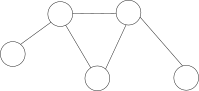
\includegraphics{undirected_graph.pdf}}\qquad	
	\subfigure[Gerichteter Graph]{\label{fig:directed_graph}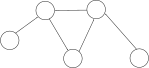
\includegraphics{directed_graph.pdf}}	
	\caption[Beispiel: Gerichteter und ungerichteter Graph]{Gerichteter und ungerichteter Graph mit $n = m = 5$.}
\end{figure}

% gewichteter Graph

\paragraph*{Gewichteter Graph} Ein gewichteter Graph (engl. \textit{weighted graph}, Abbildung \ref{fig:weighted_graph}) ist ein Tupel $G = (V,E,\omega_v,\omega_e)$. Er zeichnet sich durch die M�glichkeit aus, Gewichte an Knoten und Kanten zu definieren. Hierf�r werden die Abbildungen $\omega_v: V \rightarrow \mathbb{R}$ und $\omega_e: E \rightarrow \mathbb{R}$ verwendet.

% bezeichneter Graph
\paragraph*{Bezeichneter Graph} Ein bezeichneter Graph (engl. \textit{labeled graph}, Abbildung \ref{fig:labeled_graph}) $G=(V,E,\Sigma_V,\Sigma_E,\sigma_v,\sigma_e)$ erg�nzt Knoten- und Kantenmenge durch das Alphabet der Knotenbezeichner $\Sigma_V$, das Alphabet der Kantenbezeichner $\Sigma_E$ sowie die Abbildungen $\sigma_v: V \rightarrow \Sigma_V$ und $\sigma_e:E \rightarrow \Sigma_E$.

\begin{figure}[htb]
	\centering	
	\subfigure[Gerichteter, kantengewichteter Graph]{\label{fig:weighted_graph}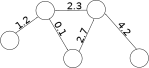
\includegraphics[scale=1.3]{weighted_graph.pdf}}\qquad	
	\subfigure[Gerichteter, bezeichneter Graph mit $\Sigma_V = \{1,2,3,4,5\}$ und $\Sigma_E = \{a,b,c,d,e\}$]{\label{fig:labeled_graph}\includegraphics[scale=1.3]{labeled_graph.pdf}}	
	\caption[Beispiel: Gewichteter und bezeichneter Graph]{Gewichteter und bezeichneter Graph.}
\end{figure}

% attributierter Graph
\paragraph*{Attributierter Graph} Ein attributierter Graph (engl. \textit{attributed graph}, Abbildung \ref{fig:attributed_graph}) verf�gt �ber die M�glichkeit, Knoten und Kanten mit zus�tzlichen Informationen in Form von Schl�ssel-Wert-Paaren zu versehen. Der Graph wird durch das Tupel \linebreak $G=(V,E,\Sigma_V, \Sigma_E, \Gamma_V, \Gamma_E, A)$ definiert, wobei $\Sigma_V$ das Alphabet aller m�glichen Schl�ssel f�r Knoteneigenschaften und $\Sigma_E$ jenes f�r alle Schl�ssel der Kanteneigenschaften bildet. $A$ ist die Menge der Eigenschaftswerte f�r Knoten und Kanten. Die Abbildung $\gamma_v: \Sigma_V \times V \rightarrow \mathcal P(A)$ ordnet die Knotenschl�ssel ihren entsprechenden Werten oder Wertemengen zu, gleiches gilt f�r Kanten unter Verwendung der Abbildung $\gamma_e: \Sigma_E \times E \rightarrow \mathcal P(A)$.

% Multigraph
\paragraph*{Multigraph} Ein Multigraph (Abbildung \ref{fig:multigraph}) ist ein Graph $G=(V,E)$, in dem die Menge aller Kanten $E$ eine Multimenge ist. Diese weist die Eigenschaft auf, dass einzelne Elemente mehrfach enthalten sein k�nnen. Somit ist die Definition beliebig vieler Kanten zwischen zwei Knoten m�glich. Zwei gerichtete Kanten gelten als \textit{parallel}, wenn sie den gleichen Start- und Zielknoten aufweisen.

\begin{figure}[htb]
	\centering	
	\subfigure[Kantenattributierter, gerichteter Graph mit $\Sigma_V = \{a,b\}$ und $A = \{1,2,3,4,5,h,o,d,r\}$]{\label{fig:attributed_graph}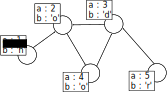
\includegraphics[scale=1.5]{attributes_graph.pdf}}\qquad	
	\subfigure[Gerichteter, kantenbezeichneter Multigraph]{\label{fig:multigraph}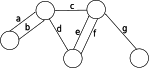
\includegraphics[scale=1.5]{multigraph.pdf}}	
	\caption[Beispiel: Attributierter Graph und Multigraph]{Attributierter Graph und Multigraph.}	
\end{figure}

Bei der Betrachtung der verschiedenen Graph-Typen wird deutlich, dass diese sich nicht zwingend gegenseitig ausschlie�en. Die Kanten in einem Multigraphen k�nnen zum Beispiel gerichtet und bezeichnet sein. Dar�ber hinaus lassen sich bezeichnete Graphen mit Hilfe von attributierten Graphen abbilden. Neben den verschiedenen Arten von Graphen sind in der vorliegenden Arbeit weitere graphentheoretische Konzepte relevant, welche im Folgenden definiert werden. Alle Definitionen beziehen sich auf gerichtete Graphen.

\paragraph*{Teilgraph, Obergraph} Ein Graph $G'=(V',E')$ hei�t Teilgraph oder Subgraph von einem Graph $G=(V, E)$, wenn $V' \subseteq V$ und $E' \subseteq E$. $G$ ist der Obergraph von $G'$. Der Teilgraph $G'$ ist \textit{induziert}, wenn er alle Kanten $(x,y) \in E$ mit $x,y \in V'$ enth�lt.

\paragraph*{Nachbarschaft} Zwei Knoten $u,v \in V$, die durch eine Kante $e = (u,v)$ verbunden sind, hei�en \textit{adjazent} oder benachbart in $G$. Die Nachbarschaft $N(v)$ eines Knotens $v$ ist die Menge aller adjazenten Knoten von $v$: 
\begin{equation}
	N(v) := \{u \mid (u,v) \in E \vee (v,u) \in E\}.
\end{equation}

\paragraph*{Au�en- und Innengrad, Grad}  Der Au�engrad $d^+(v)$ eines Knotens $v \in V$ ist die Anzahl der Kanten in E, deren Startknoten $v$ ist. Der Innengrad $d^-(v)$ von $v$ ist die Anzahl der in $v$ endenden Kanten. Der Grad $deg(v)$ eines Knotens $v \in V$ ist die Summe aus Au�engrad und Innengrad f�r diesen Knoten. Somit gilt in gerichteten Graphen:
\begin{equation}
	deg(v) := d^+(v)+d^-(v) = \left|N(v)\right|.
\end{equation}
In gewichteten Graphen werden bei der Berechnung des Grades die einzelnen Kantengewichte ber�cksichtigt.
\begin{equation}
	deg(v) := \sum_{e \in N(v)}\omega_e(e) 
\end{equation}

\paragraph*{Weg, Kantenfolge, Pfad, Kreis} Ein Weg ist eine Sequenz $v_1,e_1,v_2,e_2,...,v_{k-1},e_{k-1},v_k$ von Knoten und Kanten eines Graphen $G$. Die \textit{L�nge} des Weges ist die Anzahl der Kanten innerhalb der Sequenz. Ein Weg ist eine Kantenfolge in $G$, wenn jede Kante h�chstens einmal in dieser Folge auftritt. Gilt $v_1 = v_k$, so bezeichnet man diese Folge als \textit{geschlossen}, andernfalls handelt es sich um eine \textit{offene} Kantenfolge. Eine Kantenfolge ist ein Pfad, wenn alle Knoten innerhalb der Folge voneinander verschieden sind. Kommt mit Ausnahme von $v_k$ kein Knoten doppelt in der geschlossenen Kantenfolge vor, bezeichnet man diese als einfachen Kreis.

\paragraph*{Abstand} Der Abstand $dist(u,v)$ von zwei Knoten $u,v \in V$ ist die L�nge des k�rzesten Pfades von $u$ nach $v$. Existiert kein solcher Weg, so gilt $dist(u,v) = \infty$.

\section{Arten von Netzwerken}
\label{sec:nwarten}

Netzwerk ist ein allgemeiner Oberbegriff f�r die Beschreibung von Beziehungen zwischen Objekten. Art und Verteilung der Beziehungen definieren dabei ein Muster, anhand dessen sich Aussagen �ber das Netzwerk treffen lassen. Objekte und deren Beziehungen werden mittels Knoten und Kanten modelliert und durch graphentheoretische Algorithmen analysiert. Im Folgenden werden vier verschiedene Arten von Netzwerken nach Newman\cite{Newman:2010:NI:1809753} vorgestellt.

\textbf{Technologische Netzwerke} bilden physikalische Infrastrukturen ab. Einer der bekanntesten Vertreter ist das Internet. Hier ist das Finden effizienter Routen, auf deren Grundlage Datenpakete zwischen Knoten weitergeleitet werden, eine der wesentlichen Aufgaben. Transportnetzwerke z�hlen ebenfalls zu den technologischen Netzwerken. Orte werden als Knoten und die Verbindungen zwischen ihnen als Kanten modelliert. Eine typische Anwendung ist auch hier das Ermitteln von Routen zwischen zwei oder mehreren Orten. Dabei ist nicht immer ausschlie�lich der geographisch k�rzeste Weg von Interesse, vielmehr spielen zus�tzliche Einschr�nkungen, wie die Kombination verschiedener Transportmittel und das Meiden bestimmter Knoten (z.B. von Gro�st�dten) eine Rolle.

In \textbf{sozialen Netzwerken} stehen die Knoten f�r Personen, Gruppen oder Ereignisse, die Kanten beschreiben Beziehungen zwischen ihnen. Diese Beziehungen k�nnen sehr vielf�ltig sein, typische Beispiele sind Freundschaft, berufliche Beziehung oder Gruppenmitgliedschaft. Prominente Beispiele sind Netzwerke, wie sie im World Wide Web zu finden sind. Hierzu z�hlen zum Beispiel Facebook\footnote{\url{http://www.facebook.com}} oder LinkedIn\footnote{\url{http://www.linkedin.com/}}. Aber auch reale soziale Netzwerke, wie zum Beispiel in Schulen oder Firmen, werden dieser Kategorie zugeordnet. Der Bereich der Social Network Analysis\cite{INSNA_web} (SNA) befasst sich mit dem Aufdecken und Analysieren von Interaktionsmustern innerhalb solcher Netzwerke. Dabei ist neben der Struktur von Organisationen und sozialen Gruppen auch die Evolution der Netzwerke von Interesse. Firmen nutzen beispielsweise Ausbreitungseigenschaften von Informationen f�r virales Marketing, auch die Verbreitungswege von Krankheiten lassen sich auf dieser Grundlage untersuchen. Des Weiteren k�nnen Empfehlungen f�r neue Kontakte oder Gruppen ausgesprochen werden. Dies erfolgt auf Basis des zur�ckliegenden Nutzerverhaltens oder der aktuellen Netzwerkstruktur in der unmittelbaren Umgebung eines Knotens.

Eine weitere Kategorie bildet die Gruppe der \textbf{biologischen Netzwerke}. In vielen Bereichen der Biologie werden Netzwerke eingesetzt um das Verhalten bestimmter Elemente abzubilden. Molekularbiologen nutzen Netzwerke um chemische Reaktionen in Zellen darzustellen, Neurowissenschaftler modellieren die Verbindungen von Hirnzellen. Eine weitere Anwendung ist die Repr�sentation des Verhaltens verschiedener Spezies in �kosystemen. 

Die vierte und f�r die vorliegende Arbeit relevante Kategorie bilden die \textbf{Informations- oder Wissensnetzwerke}, oft auch als semantische Netzwerke bezeichnet. Objekte sind dabei Informationen in Form von Begriffen oder konkreten Daten, welche miteinander verkn�pft sind. Die Beziehungen werden dabei m�glichst explizit definiert\cite{semantische_netze:2010}, lassen sich aber auch aus bestehenden Beziehungen ableiten. Bestes Beispiel f�r ein Wissensnetzwerk ist das World Wide Web. Hierbei werden Webpr�senzen als Knoten und Hyperlinks als Kanten modelliert. Kanten sind gerichtet, da eine Verbindung von Webpr�senz A zu Webpr�senz B nicht zwingend eine Verbindung von B nach A voraussetzt. Eine Wichtung der Knoten ist vorstellbar in Abh�ngigkeit des Innengrades, welcher hierbei die Anzahl der eingehenden Hyperlinks auf eine Website repr�sentiert. Diese Information wird u.a. im Pagerank\cite{Brin:1998:ALH:297805.297827} Algorithmus von Google zur Wichtung von Suchergebnissen verwendet. Eng verbunden mit dem World Wide Web ist das Semantic Web\cite{SEMWEB:2013}. Schwerpunkt ist hierbei die maschinenlesbare Repr�sentation von Beziehungen zwischen beliebigen Ressourcen.\\
Ein weiteres Informationsnetzwerk, welches auch im Rahmen aktueller Forschungen in der Abteilung Datenbanken der Universit�t Leipzig untersucht wird, sind Beziehungen innerhalb von Gesch�ftsdaten\footnote{Diese Daten stammen zum Beispiel aus ERP-Systemen (engl. \textit{Enterprise Resource Planing}) und werden mit Daten aus anderen Systemen, wie zum Beispiel CRM (engl. \textit{Customer Relationship Management}) oder PM (engl. \textit{Project Management}) integriert.}. In diesen werden Stammdaten, wie zum Beispiel Mitarbeiter oder Produkte, mit transaktionalen Daten, wie zum Beispiel Rechnungen, Auftr�gen und Buchungen, verkn�pft. Die Instanzen der jeweiligen Datenart sind Knoten im Graphen, die Verkn�pfungen zwischen ihnen lassen sich durch bezeichnete Kanten ausdr�cken. Betrachtet man Teile dieses Graphen als Gesch�ftsprozess, so kann untersucht werden, worin sich Teilgraphen erfolgreicher\footnote{Ein Prozess ist zum Beispiel genau dann erfolgreich, wenn die Summe der Einnahmen innerhalb des Prozesses die Prozesskosten �berschreitet.} Prozesse von denen nicht erfolgreicher Prozesse unterscheiden. Eine detaillierte Beschreibung des Anwendungsfalls erfolgt in Abschnitt \ref{sec:anforderungen}.

\section{Klassifikation graphenbasierter Softwaresysteme}
\label{sec:graphsystems_classification}

Aus dem vorherigen Abschnitt geht hervor, dass Graphen f�r eine Vielzahl verschiedener Anwendungen eine Rolle spielen. Daraus folgt, dass auch an die Konzeption und Implementierung dedizierter Softwaresysteme unterschiedliche Anforderungen gestellt werden. Nachfolgend werden die drei Kategorien graphenbasierter Softwaresysteme beschrieben. Die Kategorisierung gr�ndet sich auf die Ausf�hrungen in \cite{Buerli:2012}, \cite{robinson2013graph} und \cite{Shao:2012:MML:2213836.2213907} sowie eigene �berlegungen im Rahmen der Arbeit.

\subsection{Graphdatenbanksysteme}
\label{subsec:gdbms}

Kemper und Eickler definieren in \cite{kemper2006datenbanksysteme} ein Datenbankverwaltungssystem (engl. \textit{database management system}, DBMS) wie folgt:

\begin{quote}
\textit{Die Gesamtheit aller Programme zum Zugriff auf die Datenbasis, zur Kontrolle der Konsistenz und zur Modifikation der Daten wird als Datenbankverwaltungssystem bezeichnet.}
\end{quote}

Unter einer \textit{Datenbasis} versteht man die gespeicherten Daten in Form von miteinander in Beziehung stehenden Informationseinheiten. 

Angles definiert in \cite{Angles:2008} ein Graphdatenbankmodell wie folgt:

\begin{quote}
\textit{Ein Graphdatenbankmodell ist ein Modell, in welchem die Datenstrukturen f�r Schema und/oder Instanzen direkt als Graph modelliert sind. Datenmanipulation erfolgt durch graphenorientierte Operationen und Typkonstruktoren, Integrit�tsbedingungen k�nnen auf der Graphstruktur definiert werden.}
\end{quote}

Ein Datenbankverwaltungssystem, welches ein Graphdatenbankmodell implementiert, wird im Rahmen dieser Arbeit als \textbf{Graphdatenbankverwaltungssystem} (engl. \textit{graph database management system}, GDBMS) bezeichnet. Eine \textit{Graphdatenbank} ist die Instanz eines Graphen und stellt somit die vom GDBMS verwaltete Datenbasis dar. 
%Der von Angles verwendete Begriff der Datenstruktur wird allgemeiner als \textit{Datenmodell} bezeichnet (Abschnitt \ref{sec:datamodels}). 
Nachfolgend werden die Begriffe Graphdatenbanksystem und Graphdatenbankverwaltungssystem im Text synonym verwendet.

Graphdatenbanksysteme sind generell f�r den Einsatz als OLTP-System (engl. \textit{Online Transaction Processing}) konzipiert\cite{robinson2013graph}. Der Schwerpunkt liegt somit auf Mehrbenutzerf�higkeit, transaktionaler Performance, Integrit�t und Verf�gbarkeit. GDBMS eignen sich vorrangig f�r die Ausf�hrung lokaler Operationen, diese betrachten nur einen Teil des Graphen, wie zum Beispiel die Umgebung eines definierten Knotens oder einer Knotenmenge.

Festzuhalten ist, dass sich ein GDBMS �ber drei wesentliche Aufgaben definiert:
\begin{enumerate}
	\item Bereitstellen von Informationen als Instanz eines graphenspezifischen Datenmodells
	\item Bereitstellen von Operationen zur Definition, Manipulation und Abfrage einer Instanz des Datenmodells
	\item Sicherstellen der Widerspruchsfreiheit innerhalb der Datenbasis
\end{enumerate}

Ausgehend von dieser allgemeinen Definition lassen sich die vorhandenen Systeme weiter unterteilen. Nachfolgend werden die im Rahmen der Arbeit relevanten Auspr�gungen von GDBMS erl�utert.

\paragraph*{Native versus nicht-native GDBMS}

Als native GDBMS bezeichnet man jene Systeme, in denen sowohl die Verarbeitung als auch die Speicherung der Datenbasis graphenorientiert erfolgt\cite{robinson2013graph}. Im Sinne der Verarbeitung spielt hierbei das Konzept der \textit{indexfreien Adjazenz}\cite{DBLP:journals/corr/abs-1004-1001} eine entscheidende Rolle. Zum Verst�ndis soll kurz die Modellierung von Netzwerken im relationalen Datenmodell\cite{Codd:1970:RMD:362384.362685} skizziert werden. In RDBMS werden Beziehungen zwischen Objekten durch Fremdschl�sselattribute und im Fall von $n:m$ Beziehungen durch zus�tzliche Tabellen (engl. \textit{mapping tables}) abgebildet. Im Zuge der Normalisierung entsteht eine gro�e Anzahl von Tabellen, welche �ber Fremdschl�sselbeziehungen miteinander verbunden sind. F�r die Verwaltung stark vernetzter Daten weist dieses Modell einen entscheidenden Nachteil auf: Im Falle einer Selektion m�ssen die Tabellen unter der Verwendung von Verbundoperationen (sog. JOIN-Operationen) wieder zusammengefasst werden, um die angeforderte Teilmenge zu extrahieren. Relationale Datenbanken begegnen diesem Problem mittels Anfrageoptimierung, dem Einsatz von Cachingstrategien oder der Verwendung von Indizes auf Fremdschl�sselattributen\cite{haerder2001datenbanksysteme}. Der Aufwand, einen Index nach einem bestimmten Schl�ssel zu durchsuchen steht meist in einem logarithmischen Verh�ltnis zur Anzahl der hinterlegten Eintr�ge. Der Aufwand vervielfacht sich, wenn mehrere JOIN-Operationen rekursiv hintereinander ausgef�hrt werden m�ssen.\\
Native GDBMS hingegen bilden die Daten in ihrer expliziten Struktur ab, Beziehungen zwischen Objekten werden durch Kanten modelliert und als Referenz direkt am Objekt abgelegt. Der geringe Aufwand, die Nachbarschaft eines Knotens zur Laufzeit abzufragen, ist der entscheidende Vorteil, den diese Struktur aufweist. W�hrend bei einer JOIN-Operation typischerweise ein Index in die Berechnung einbezogen wird, ist die Komplexit�t dieser Operation in einem nativen GDBMS nur vom aktuellen Knotengrad abh�ngig. Somit bleibt sie unabh�ngig von der Gr��e des Graphen konstant. Die Kanten innerhalb des Graphen k�nnen als materialisiertes Ergebnis einer JOIN-Operation verstanden werden. Gegen�ber einem relationalen DBMS f�hrt dies insbesondere bei rekursiven Anfragen gro�er Tiefe, wie zum Beispiel der Pfadsuche, zu einem entscheidenden Geschwindigkeitsvorteil.

Die M�glichkeit zur nativen Verarbeitung ist eng verkn�pft mit der Repr�sentation des Graphen im Hauptspeicher und auf Externspeichern. Eine hohe Performance rekursiver Anfragen kann nur erreicht werden, wenn der direkte Zugriff auf die Nachbarschaft eines Knotens auch physisch effizient m�glich ist. Native GDBMS speichern den Graphen in einem Format, dass f�r rekursive Operationen optimiert ist. In \cite{Shao:2012:MML:2213836.2213907} wird diskutiert, dass es keine Repr�sentation des Graphen geben kann, welche f�r alle vorstellbaren Graphalgorithmen optimal ist, da Zugriffe innerhalb des Graphen grunds�tzlich wahlfrei sind. Ungeachtet dessen existieren verschiedene Datenformate zur effizienten Verarbeitung des Graphen, diese sind jedoch nur hinsichtlich bestimmter Operationen optimiert.

Nicht-native GDBMS sind jene Systeme, welche die Modellierung der Daten als Graph unterst�tzen, f�r die Verarbeitung und Speicherung jedoch auf andere Technologien zur�ckgreifen. Dazu z�hlen zum Beispiel relationale und objektorientierte Datenbanken aber auch dedizierte Persistenzframeworks\cite{robinson2013graph}. Nicht-native GDBMS weisen den Vorteil auf, dass viele der zugrundeliegenden Systeme durch eine lange Entwicklungsdauer und den oft mehrj�hrigen Einsatz als Produktivsystem eine hohe Stabilit�t aufweisen und deren Funktionsweise umfassend dokumentiert ist. Nicht-native Verarbeitung weist bei traversierenden Anfragen Leistungsdefizite auf, daf�r k�nnen andere Anfragen, wie zum Beispiel mengenorientierte, von einer entsprechend optimierten Verarbeitung profitieren.

\paragraph*{Zentrale versus verteilte GDBMS} 

Ein weitere Differenzierung von GDBMS ist die klassische Einteilung in zentrale und verteilte Systeme. Zentrale GDBMS werden auf einem einzelnen, zentralen Rechner ausgef�hrt. Steigenden bzw. generell hohen Anforderungen hinsichtlich Anfragelast und verwalteter Datenmenge kann in diesen Systemen durch \textit{vertikale Skalierung} (engl. \textit{scale up}) begegnet werden\cite{DBLP:journals/corr/cs-AR-9912010}. Hierbei wird durch das �ndern der Hardwarekonfiguration, wie zum Beispiel dem Hinzuf�gen mehrerer, leistungsf�higerer Prozessoren oder gr��erer Mengen an Hauptspeicher, die Leistung des Systems gesteigert. Die maximale Leistungsf�higkeit ist damit durch die technische Entwicklung im Bereich der Hardware und durch die Wirtschaftlichkeit der eingesetzten Ressourcen limitiert.

Ein Weg, der Forderung nach hoher Leistungsf�higkeit zu begegnen, ist der Einsatz verteilter GDBMS. Diese zeichnen sich dadurch aus, dass Instanzen eines konkreten GDBMS auf mehreren Rechnern parallel ausgef�hrt werden. F�r die Beantwortung von Anfragen und die Verwaltung der Datenbasis kooperieren die einzelnen Instanzen. Eine Steigerung der Leistungsf�higkeit wird durch das Hinzuf�gen zus�tzlicher Rechner oder Instanzen erreicht. Dieses Vorgehen wird als \textit{horizontale Skalierung} (engl. \textit{scale out}) bezeichnet\cite{DBLP:journals/corr/cs-AR-9912010}. Ziel dabei ist eine lineare Steigerung der Leistungsf�higkeit in Abh�ngigkeit zur Anzahl der hinzugef�gten Rechner\cite{rahm1994mehrrechner}. 
%Die f�r die vorliegende Arbeit relevanten GDBMS implementieren eine \textit{shared-nothing}-Architektur, diese zeichnet sich durch einen lose gekoppelten Rechnerverbund aus, in dem jedem beteiligten Rechner eigene Hardware-Ressourcen zur Verf�gung stehen\cite{rahm1994mehrrechner}.

Bei der Aufteilung der Datenbasis in verteilten Systemen unterscheidet man zwei Techniken: \textit{Replikation} und \textit{Partitionierung}. Im Rahmen einer vollst�ndigen Replikation wird die gesamte Datenbasis an allen beteiligten Rechnern redundant hinterlegt. Dies erh�ht die Verf�gbarkeit des Gesamtsystems und erm�glicht das horizontale Skalieren lesender Zugriffe. Vollst�ndige Replikation weist den Nachteil auf, dass die Datenmenge durch die Kapazit�t der einzelnen Rechner limitiert ist.\\
Die Partitionierung teilt die Datenbasis in mehrere Fragmente auf, diese werden den beteiligten Rechnern zugewiesen. Die Folgen sind eine horizontale Skalierbarkeit schreibender Zugriffe und eine theoretisch unbeschr�nkte Gr��e der Datenbasis. Mit dem Ziel, beide Zugriffsarten skalieren und gleichzeitig Verf�gbarkeit sicherstellen zu k�nnen, werden die Fragmente im Rahmen der partiellen Replikation redundant gespeichert\cite{rahm1994mehrrechner}.

\paragraph*{Eingebettete versus Client-Server GDBMS}

Viele der aktuell verf�gbaren GDBMS k�nnen als eingebettete Datenbanksysteme verwendet werden. Die Einbettung erfolgt in Form spezieller Softwarebibliotheken innerhalb des Anwendungsprogramms, die Funktionen des GDBMS k�nnen �ber herstellerspezifische APIs in Anspruch genommen werden. Eingebettete Datenbanksysteme eignen sich insbesondere f�r den Einsatz in speziellen Ger�ten oder eigenst�ndigen Desktopanwendungen. Das Anwendungsprogramm �bernimmt die Verantwortung �ber das GDBMS, eine manuelle Installation oder Aktualisierung ist nicht erforderlich. Ein wesentlicher Vorteil der eingebetteten Verwendung ist die geringe Latenz beim Aufruf von Datenbankfunktionen. Ein m�glicher Nachteil ist die Bindung an den Prozess des Anwendungsprogramms, mit welchem sich das GDBMS Ressourcen, wie zum Beispiel den verf�gbaren Hauptspeicher, teilen muss. Ein weiterer Nachteil ist die Einschr�nkung in der Wahl der Programmiersprache, da die Softwarebibliotheken typischerweise nur in der Programmiersprache des jeweiligen GDBMS zur Verf�gung stehen.

Neben der Einbettung in das Anwendungsprogramm bieten viele GDBMS-Hersteller auch die Verwendung eines eigenst�ndigen Datenbankservers an. Generell werden Datenbanksysteme h�ufig als Client-Server-Systeme realisiert\cite{vossen2008datenmodelle}. Ein Client sendet eine Anfrage an einen Server, dieser bearbeitet die Anfrage und sendet eine Antwort an den Client zur�ck. Client- und Serverprozess sind entkoppelt, was zur Folge hat, dass mehrere Clients gleichzeitig mit dem Server kommunizieren k�nnen. Die Kommunikation erfolgt auf Basis der Protokolle des jeweiligen Datenbanksystems. Viele Graphdatenbanksysteme nutzen standardisierte Protokolle f�r die Kommunikation zwischen Client und Server. Infolgedessen ist die Verwendung des GDBMS grunds�tzlich unabh�ngig von Plattform und Programmiersprache. Ein Nachteil der Client-Server-Architektur ist die h�here Latenz durch den zus�tzlichen Kommunikationsaufwand. Dar�ber hinaus zieht der Einsatz eines Datenbankservers auch entsprechende administrative Aufgaben nach sich.

\paragraph*{Disk- versus hauptspeicher-zentrierte GDBMS}

Ein weiteres wichtiges Unterscheidungsmerkmal zwischen GDBMS-Implementierungen ist die Wahl des prim�ren Speichermediums f�r die hinterlegten Daten. Generell wird in disk-zentrierte (engl. \textit{disk resident}) und hauptspeicher-zentrierte (engl. \textit{main memory based} oder \textit{in-memory}) DBMS unterschieden\cite{Garcia-Molina:1992:MMD:627289.627538}.

Disk-zentrierte DBMS stellen die klassische Form eines Datenbanksystems dar. Ihre Entwicklung erfolgte unter der Vorgabe, dass die gesamte Datenbasis auf mechanischen Festplatten hinterlegt und einzelne Fragmente bei Bedarf zur Verarbeitung in den Hauptspeicher geladen werden. Die Zugriffszeiten des Hauptspeichers sind wesentlich k�rzer als die von Festplatten. Ein wahlfreier Zugriff auf die Informationen im Hauptspeicher ist demnach effizienter als das wahlfreie Lesen von Daten auf den rotierenden Magnetscheiben einer Festplatte. DBMS-Hersteller begegneten diesem Problem mit sequentieller, an der Blockstruktur der Festplatten orientierten Datenspeicherung und dem Einsatz gro�er Datenbankpuffer mit entsprechenden Ersetzungsverfahren\cite{haerder2001datenbanksysteme}.

Hauptspeicher-zentrierte DBMS verwalten die gesamte Datenbasis innerhalb des physischen Hauptspeichers. Die eingesetzten Algorithmen und Datenstrukturen sind auf die Kommunikation zwischen Hauptspeicher, Prozessor-Caches und CPU-Registern optimiert. Durch die geringen Zugriffszeiten wird weniger die sequentielle Anordnung der Daten priorisiert, vielmehr wird versucht, durch Komprimierung mehr Daten im Hauptspeicher verwalten zu k�nnen\cite{plattner2011memory}. Hauptspeicher-zentrierte Verarbeitung ist nicht gleichbedeutend mit der Verwendung gro�er Puffer, welche den gesamten Datenbestand eines disk-zentrierten Systems aufnehmen k�nnen. Der Puffer stellt eine zus�tzliche Indirektion im Zugriff dar, Adressen m�ssen �bersetzt, das Vorhandensein des entsprechenden Blocks im Puffer gepr�ft und das angeforderte Tupel letztendlich ausgelesen werden. Diese Schritte entfallen bei einer hauptspeicher-zentrierten Verarbeitung.

Ein wesentlicher Nachteil des Hauptspeichers ist dessen Fl�chtigkeit. Wird die Stromversorgung unterbrochen, sind die hinterlegten Informationen verloren. Die Systeme nutzen zwar den Hauptspeicher als prim�res Speichermedium, setzen jedoch h�ufig Externspeicher f�r Backups ein. Insbesondere die Verwendung von Solid-State-Disks (SSD) bietet hier wesentliche Performance-Vorteile gegen�ber mechanischen Festplatten. 
%Durch die Wirtschaftlichkeit gro�er Mengen an Hauptspeicher erlangen In-Memory-DBMS zunehmend an Bedeutung. 
Wie bereits erw�hnt, erfolgt der Zugriff innerhalb des Graphen grunds�tzlich wahlfrei. Infolgedessen stellen hauptspeicher-zentrierte Implementierungen vor allem im Bereich der GDBMS eine interessante Alternative dar.

Die vorgestellten Auspr�gungen von Graphdatenbanksystemen schlie�en sich nicht zwingend gegenseitig aus, Kombinationen der einzelnen Arten sind m�glich. So ist es vorstellbar, dass ein hauptspeicher-zentriertes GDBMS als Client-Server-System eingesetzt wird oder native GDBMS in Desktopanwendungen eingebettet sind.

\subsection{Graph Processing Systems}
\label{subsec:graph_processing}

Eine zweite Art graphenbasierter Softwaresysteme sind diejenigen, welche sich mit der verteilten Analyse umfangreicher Graphen befassen. Sie werden als Graph Processing Systems (GPS) oder alternativ auch als Graph Compute Systems bezeichnet\cite{Malewicz:2010:PSL:1807167.1807184, robinson2013graph}. Ein umfangreicher Graph weist die Eigenschaft auf, dass seine Knoten- und Kantenmenge nicht mehr effizient auf einer einzelnen Maschine verarbeitet werden kann.

Anders als Graphdatenbanksysteme eignen sich GPS f�r Berechnungen, welche den gesamten Graphen ber�cksichtigen. Ein Beispiel hierf�r ist der Page-Rank-Algorithmus\cite{Brin:1998:ALH:297805.297827} von Google, welcher jeder Website einen globalen Rang auf Basis ihrer Nachbarschaft und weiteren Faktoren zuweist. Bei der Analyse sozialer Netzwerke ist zum Beispiel die Berechnung der Zentralit�t eines Knotens interessant: F�r jedes m�gliche Nutzerpaar werden die k�rzesten Pfade bestimmt um anschlie�end den Anteil jener Pfade zu berechnen, welche durch einen konkreten dritten Nutzer verlaufen.

Eine weitere Eigenschaft dieser Systeme ist die batch-orientierte Datenverarbeitung. Die Daten werden von einer externen Quelle geladen, auf mehrere Rechner verteilt, verarbeitet und das Ergebnis der Verarbeitung ausgegeben oder aber in einer nachfolgenden Berechnung weiterverwendet. Dies ist ein wesentlicher Unterschied zur Definition eines operationalen Graphdatenbanksystems, welches die Datenbasis selbst verwaltet, den interaktiven Zugriff erm�glicht und Konsistenz sicherstellt. Durch die batch-orientierte Verarbeitung k�nnen GPS eher mit OLAP-Systemen (engl. \textit{online analytical processing}) verglichen werden.

GPS werden im Rahmen dieser Arbeit nicht betrachtet, da ihr Einsatzzweck nicht zu den gestellten Anforderungen passt. Hierzu z�hlen u.a. der interaktive Zugriff und der lokale Bezug von Anfragen. Bekannte GPS-Vertreter sind die quelloffenen Projekte Apache Giraph\footnote{\url{http://giraph.apache.org/}} und Phoebus\footnote{\url{https://github.com/xslogic/phoebus}}. Beide Systeme implementieren das von Google vorgestellte Pregel-Modell\cite{Malewicz:2010:PSL:1807167.1807184}, welches unter anderem f�r die Berechnung des Page-Rank-Algorithmus eingesetzt wird und im Gegensatz zu anderen Systemen Ausf�lle von Rechnern w�hrend der Verarbeitung toleriert. MapReduce\cite{Dean:2008:MSD:1327452.1327492} ist ebenfalls ein verteiltes Berechnungsmodell f�r gro�e Datenmengen. Apache Hadoop\footnote{\url{http://hadoop.apache.org/}} ist eine bekannte Implementierung des Modells und wird im Rahmen des Pegasus-Projektes\footnote{\url{http://www.cs.cmu.edu/~pegasus/}} f�r die Berechnung von Graphalgorithmen auf umfangreichen Graphen eingesetzt.

\subsection{Software zur Analyse und Visualisierung}

Die dritte Kategorie graphenbasierter Softwaresysteme bilden unterst�tzende Werkzeuge zur Analyse und bzw. oder Visualisierung von Graphen. Es handelt sich um zentral ausf�hrbare oder als Softwarebibliothek verwendbare Programme. Die Gr��e der unterst�tzten Graphen ist durch die zur Verf�gung stehenden Menge an Hauptspeicher begrenzt. Die Systeme selbst bieten keine Unterst�tzung f�r eine automatische Datenverwaltung, Mehrbenutzerf�higkeit oder Konsistenzerhaltung an. Der analytische Funktionsumfang variiert je nach System, so werden typischerweise die Berechnung globaler Eigenschaften, wie zum Beispiel die Dichte\footnote{Die Dichte eines Graphen beschreibt das Verh�ltnis zwischen der Anzahl von Kanten und der maximal m�glichen Anzahl von Kanten\cite{DBLP:books/daglib/0030488}.} des Graphen, der durchschnittliche Grad oder die Anzahl maximal zusammenh�ngender Teilgraphen\footnote{Ein Graph ist zusammenh�ngend, wenn alle m�glichen Knotenpaare innerhalb des Graphen durch einen Weg verbunden sind\cite{DBLP:books/daglib/0030488}.} genauso unterst�tzt wie lokale Operationen. Letztere umfassen zum Beispiel das Berechnen k�rzester Pfade oder maximaler Fl�sse.

Die Visualisierung von Graphen stellt ebenfalls ein wichtiges Forschungsgebiet dar\cite{kaufmann2001drawing}. Die grafische Aufbereitung komplexer Netzwerke kann dem Endanwender das Verst�ndnis erleichtern und auch neue Erkenntnisse �ber Eigenschaften oder Besonderheiten des Graphen erm�glichen. Verschiedene Layout-Algorithmen werden in den jeweiligen Systemen implementiert, um je nach Topologie des Graphen die optimale Visualisierung w�hlen zu k�nnen. Einige der Systeme stellen Erweiterungen f�r die Kommunikation mit GDBMS zur Verf�gung, wodurch die im Datenbanksystem hinterlegten Daten visualisiert werden k�nnen.

Die dritte Kategorie graphenbasierter Softwaresysteme wird im Rahmen der vorliegenden Arbeit nicht betrachtet, da die Systeme f�r die dauerhafte Datenverwaltung ungeeignet sind. Beispiele f�r Softwaresysteme zur Analyse und Visualisierung sind JUNG\footnote{\url{http://jung.sourceforge.net/}}, GraphViz\footnote{\url{http://www.graphviz.org/}} und Gephi\footnote{\url{https://gephi.org/}}.

\section{Datenmodelle in GDBMS}
\label{sec:datamodels}

Datenbankmanagementsysteme implementieren ein Datenmodell, welches die Modellierungskonstrukte festlegt, mittels derer ein Informationsabbild der realen Welt generiert werden kann. Ein Datenbankmodell ist somit eine Form der Abstraktion und bietet die M�glichkeit zur Modellierung von Datenobjekten und zur Festlegung der anwendbaren Operatoren und deren Wirkung\cite{elmasri2009grundlagen, kemper2006datenbanksysteme}. Die in GDBMS h�ufig eingesetzten Datenmodelle sind das Property-Graph-Modell und das Hypergraph-Modell. Im Bereich des Semantic Web findet das Resource Description Framework zur Modellierung von Graphen Anwendung.

\subsection{Property-Graph-Modell}
\label{subsec:propgraph}

Das Property-Graph-Modell (PGM) ist ein gerichteter, kantenbezeichneter, attributierter Multigraph\cite{DBLP:journals/corr/abs-1006-2361, DBLP:journals/corr/abs-1004-1001}. Formal betrachtet l�sst sich dieser als ein Tupel in der Form \linebreak$G = (V,E,\Sigma_{E_L}, \Sigma_{V_A}, \Sigma_{E_A}, A, \sigma_e, \gamma_v, \gamma_e)$ definieren. $\Sigma_{E_L}$ beschreibt das Alphabet der Kantenbezeichner, dessen Symbole durch die Abbildung $\sigma_e:E \rightarrow \Sigma_{E_L}$ den Kanten zugeordnet werden. $\Sigma_{V_A}$ bzw. $\Sigma_{V_E}$ bilden die Schl�sselalphabete, $A$ die Wertemenge f�r Knoten- bzw. Kantenattribute. Die Abbildungen $\gamma_v: \Sigma_{V_A} \times V \rightarrow \mathcal P(A)$ und $\gamma_e: \Sigma_{V_E} \times E \rightarrow \mathcal P(A)$ ordnen die Knotenschl�ssel ihren entsprechenden Werten oder Wertemengen zu. 

Gro�er Vorteil des PGM ist dessen Flexibilit�t hinsichtlich der Abbildung verschiedener Arten von Graphen\cite{DBLP:journals/corr/abs-1006-2361}. Neben der grundlegenden ungerichteten Form ohne zus�tzliche Eigenschaften, l�sst sich jede Kombination aus gerichteten, gewichteten und attributierten Graphen und Multigraphen darstellen. Das Modell eignet sich somit zur Repr�sentation einer Vielzahl der im vorhergehenden Abschnitt vorgestellten Netzwerke.

Das Modell sieht keine strenge Typisierung von Knoten und Kanten vor, d.h. deren Attribute sind grunds�tzlich nicht durch ein Schema festgelegt und k�nnen damit beliebig auf Instanzebene vergeben werden. Es handelt sich demnach um ein semistrukturiertes Modell, da keine explizite Unterscheidung zwischen Strukturinformationen und Daten vorgenommen wird, sondern vielmehr jede Instanz eines Knotens bzw. einer Kante die jeweiligen Informationen in sich vereint. Der sich daraus ergebende Vorteil ist die hohe Flexibilit�t zum Einen gegen�ber der Schemaevolution an Knoten und Kanten innerhalb des Modells und zum Anderen im Datenaustausch zwischen verschieden modellierten Datenquellen. In diversen Anwendungen kann es jedoch sinnvoll sein, den Typ eines Knotens zu modellieren. Auf logischer Ebene erlaubt dies eine semantisch eindeutige Beschreibung der einzelnen Instanzen, auf physischer Ebene die Definition von Indizes und Konsistenzkriterien oder die Ber�cksichtigung des Typen im Rahmen der Anfrageoptimierung\cite{EdlichFriedlandHampeBrauer201010}. Eine M�glichkeit der Realisierung ist der Einsatz dedizierter Attributschl�ssel, wie zum Beispiel \texttt{Type}. Die Zust�ndigkeit f�r Definition und Einhaltung eines Schemas liegt in diesem Fall bei der Anwendung. Einige GDBMS bieten die M�glichkeit Knoten- und Kantentypen zu definieren und �bernehmen somit ihrerseits die Verantwortung f�r die Einhaltung anwendungsspezifischer und modellinh�renter Integrit�tsbedingungen.

Abbildung \ref{fig:propertygraph} zeigt am Beispiel eines sozialen Netzwerkes die Instanz eines Property-Graphen. Personen stehen miteinander �ber Freundschaften in Beziehung, studieren an Hochschulen oder sind Mitglied in Vereinen, die wiederum von Hochschulen betreut werden. Knotenattribute werden in der Form \texttt{Schl�ssel : Wert} dargestellt. Die Knotentypen Hochschule, Person und Verein sind farblich voneinander abgehoben, der jeweilige Typ wird durch den Attributschl�ssel \texttt{Type} definiert. Das Beispiel verzichtet auf Kantenattribute, vorstellbar w�ren aber zum Beispiel die Rolle einer Person in einem Verein oder Datumsangaben, welche den Erstellungszeitpunkt der Beziehung dokumentieren.

\begin{figure}[htb] 
	\centering
		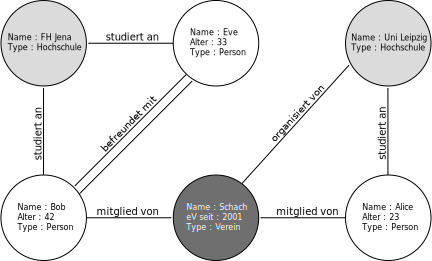
\includegraphics{PropertyGraph.pdf}
	\caption[Beispiel: Property-Graph]{Beispiel eines Property-Graphen mit den drei Knotentypen Hochschule, Verein und Person, welche �ber verschiedene Kantentypen in Relation miteinander stehen.}
	\label{fig:propertygraph}
\end{figure}

Bis auf wenige Ausnahmen wird das Property-Graph-Modell in nahezu allen kommerziell verf�gbaren GDBMS eingesetzt\cite{EdlichFriedlandHampeBrauer201010}. Teilweise wird das Modell modifiziert, ein Beispiel hierf�r sind explizite Knotenbezeichner in Neo4j 2.0\cite{Neo4j_web_labels:2013}.

\subsection{Hypergraph-Modell}

Die zu Beginn des Kapitels betrachteten Graphen-Definitionen sowie das PGM erlauben ausschlie�lich bin�re Beziehungen zwischen Objekten, d.h. eine Kante verbindet genau zwei Knoten. Es existieren jedoch Anwendungsgebiete, in denen die Modellierung von Relationen h�herer Ordnung von Interesse ist. Ein Beispiel hierf�r ist die Wissensrepr�sentation, welche unter anderem in den Bereichen k�nstliche Intelligenz, Bioinformatik und Computerlinguistik eingesetzt wird\cite{Iordanov:2010:HGG:1927585.1927589}. Relationen h�herer Ordnung, welche auch als n-�re Beziehungen bezeichnet werden, lassen sich durch mehrere bin�re Relationen ausdr�cken. Dies erh�ht jedoch die Komplexit�t und Fehleranf�lligkeit der Repr�sentation und verringert gleichzeitig deren Verst�ndlichkeit und �bersichtlichkeit. In Hypergraphen wird von dieser Komplexit�t abstrahiert, indem mehrere bin�re Relationen in Hyperkanten zusammengefasst werden.

Das Hypergraph-Modell (HGM) beschreibt einen Hypergraph $H=(V,E)$ bestehend aus einer Menge $V=\{v_1,v_2,\ldots,v_n\}$ von Knoten und einer Menge $E = \{E_1,E_2,\ldots E_m\} = \mathcal P(V) \setminus \emptyset$ von Hyperkanten, wobei $E_i \subseteq V$ f�r $i=1,\ldots,m$. Eine gerichtete Hyperkante ist ein geordnetes Paar $E = (A,B)$ mit $A,B \subseteq V$ und $A \cap B = \emptyset$. Ein gerichteter Hypergraph besteht aus gerichteten Hyperkanten\cite{Gallo:1993:DHA:153578.153586}.

\begin{figure}[htb] 
	\centering
		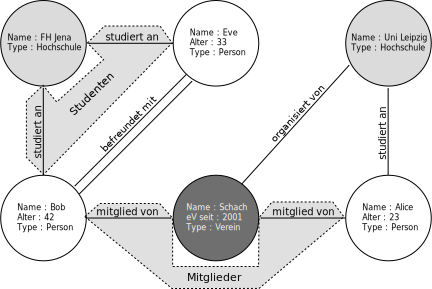
\includegraphics{PropertyHyperGraph.pdf}
	\caption[Beispiel: Property-Hypergraph]{Beispiel eines Property-Hypergraphen mit zwei gerichteten Hyperkanten $\texttt{Studenten} = (\{\texttt{Eve}, \texttt{Bob}\}, \{\texttt{FH Jena}\})$ und $\texttt{Mitglieder} = (\{\texttt{Alice}, \texttt{Bob}\}, \{\texttt{Schach}\})$.}
	\label{fig:propertyhypergraph}
\end{figure}

Abbildung \ref{fig:propertyhypergraph} greift das Beispiel des sozialen Netzwerkes erneut auf. Die bin�ren Relationen \texttt{studiert an} und \texttt{mitglied von} werden zu den gerichteten Hyperkanten \texttt{Studenten} und \texttt{Mitglieder} zusammengefasst. Am Beispiel wird deutlich, dass auch Knoten, Kanten und Hyperkanten in Hypergraphen mit Attributen und Bezeichnern versehen werden k�nnen. Ein Property-Graph-Modell mit der M�glichkeit, Relationen h�herer Ordnung zu definieren, wird als Property-Hypergraph-Modell (PHGM) bezeichnet und weist die gleichen Eigenschaften bez�glich Strukturiertheit bzw. Typisierung wie das PGM auf.

Im Vergleich zum PGM ist das HGM in kommerziellen GDBMS wenig verbreitet. Ein Vertreter ist das Graphdatenbanksystem HypergraphDB, welches das HGM um ein Typsystem und die M�glichkeit Hyperkanten auf Hyperkanten zeigen zu lassen erweitert\cite{Iordanov:2010:HGG:1927585.1927589}.

\subsection{Resource Description Framework}
\label{subsec:rdf}

Das Resource Description Framework\cite{RDF:2013} (RDF) ist ein vom World Wide Web Consortium (W3C) standardisiertes Datenmodell f�r die Formulierung und den Austausch von Aussagen �ber beliebige Dinge, welche innerhalb des Modells als Ressourcen bezeichnet werden. RDF wurde im Umfeld des Semantic Web\cite{SEMWEB:2013} entwickelt, dieses widmet sich der semantischen Auszeichnung von Informationen und deren maschineller Interpretation und Verarbeitung.

Eine Aussage ist als ein Tripel bestehend aus Subjekt, Pr�dikat und Objekt definiert. Das Subjekt ist die zu beschreibende Ressource, das Pr�dikat definiert eine Eigenschaft des Subjektes und das Objekt den Wert dieser Eigenschaft. Pr�dikate sind ebenfalls Ressourcen, Objekte k�nnen entweder Ressource oder Literal sein. Eine Menge von Aussagen zu einem Subjekt bildet somit dessen Beschreibung. Eine Ressource wird durch einen Uniform Resource Identifier (URI) eindeutig identifiziert. F�r die automatisierte maschinelle Verarbeitung ist diese Eindeutigkeit obligatorisch, da sie Mehrdeutigkeiten und folglich Fehlinterpretationen verhindert\cite{DBLP:journals/dlib/Miller98}. 

Aus mathematischer Sicht betrachtet ist das RDF-Modell ein gerichteter, bezeichneter Multigraph. Ein wesentlicher Unterschied zum PGM besteht darin, dass Knoten- und Kanteneigenschaften durch dedizierte Tripel modelliert werden m�ssen. Eine modellinh�rente Differenzierung in eine Beziehung zwischen Ressourcen und einer Beschreibung einer einzelnen Ressource ist dabei nicht gegeben. Das Modell erfordert keine strenge Typisierung und eignet sich somit genau wie PGM und HGM f�r die Speicherung semistrukturierter Daten. Abbildung \ref{fig:rdfgraph} zeigt dies am Beispiel eines sozialen Netzwerkes.

\begin{figure}[htb] 
	\centering
		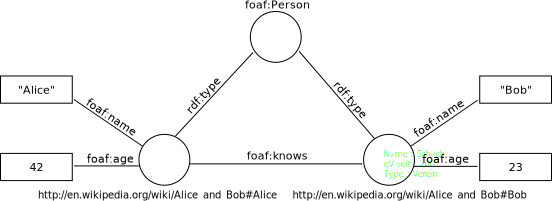
\includegraphics{RDFGraph.pdf}
	\caption[Beispiel: RDF-Instanz]{Instanz eines RDF-Modells am Beispiel eines sozialen Netzwerkes. Gezeigt werden die Ressourcen Alice  und Bob, welche durch die entsprechenden Wikipedia-URIs eindeutig bestimmt sind. Ihre Beziehung wird durch das Pr�dikat \texttt{foaf:knows} beschrieben. Beide Ressourcen sind vom Typ \texttt{foaf:Person}. Die Beziehungen selbst sind ebenfalls Ressourcen, Friend-of-a-friend (\texttt{foaf}) repr�sentiert den Namensraum \texttt{http://xmlns.com/foaf/spec/}, das Prefix \texttt{rdf} den Namensraum \texttt{http://www.w3.org/1999/02/22-rdf-syntax-ns\#}. Die Beschreibung von Alice und Bob wird durch deren Beziehungen zu den Literalen \texttt{Alice} und \texttt{42} bzw. \texttt{Bob} und \texttt{23} erg�nzt.}
	\label{fig:rdfgraph}
\end{figure}

F�r die Manipulation und den Zugriff auf Daten im RDF-Modell wird die graphenbasierte Anfragesprache SPARQL\cite{SPARQL:2013} entwickelt und eingesetzt. Deren grundlegender Ansatz ist die Definition eines Teilgraphen als Muster, nach welchem die Datenbasis durchsucht wird. Innerhalb des Musters k�nnen Variablen definiert werden, diese werden w�hrend der Anfrageverarbeitung instanziiert. Wird das Muster in der Datenbasis gefunden, besteht die Ergebnismenge aus den definierten Variablen und deren Belegung.

Einer der Schwerpunkte des Semantic Web ist das Ableiten neuer Beziehungen zwischen Ressourcen auf der Basis vorhandener Informationen und zus�tzlich definierter Regeln. Dieses Vorgehen wird auch als Inferenz bezeichnet\cite{Inference:2013}. Ein zweiter Schwerpunkt ist das Konzept des Linked Data\cite{linked_data:2013}. Es beschreibt, wie eigenst�ndige Datenquellen im Web virtuell zusammengef�hrt und quellen�bergreifende Beziehungen zwischen den Ressourcen definiert werden. Mit Hilfe dieser umfassenden,  virtuell integrierten Datenbasis k�nnen komplexe Anfragen beantwortet und neue Informationen abgeleitet werden.

F�r die Speicherung von RDF-Daten werden entweder spezielle Datenbanksysteme, sog. Triple-Stores, eingesetzt oder aber bestehende Datenbanksysteme, wie zum Beispiel \linebreak RDBMS, mit entsprechender Funktionalit�t erweitert. Beide Systemarten unterst�tzen nicht die im vorhergehenden Abschnitt definierte indexfreie Adjazenz und z�hlen somit zu den nicht-nativen GDBMS\cite{robinson2013graph}. Die Systeme selbst bieten SPARQL-Endpunkte an, �ber welche auf die hinterlegte Datenbasis zugegriffen werden kann.

Das RDF-Modell und SPARQL geh�ren zu den grundlegenden Komponenten des Semantic Web. Wie bereits erw�hnt, sind die wesentlichen Einsatzszenarien das Ableiten neuer Beziehungen und das virtuelle Integrieren von Daten aus verschiedenen Quellen. Diese Szenarien sind jedoch nicht wesentlich f�r die vorliegende Arbeit. Aus technischer Sicht sind RDF-Datenbanksysteme f�r das schnelle Auffinden statischer Muster innerhalb der Datenbasis optimiert\cite{de2013choosing}. Insbesondere f�r die Analyse von Netzwerken ist jedoch das dynamische Traversieren von Graphen relevant. Hierf�r eignen sich RDF-Datenbanksysteme weniger als native GDBMS, welche das PGM implementieren und f�r das Traversieren von Graphen optimiert sind\cite{robinson2013graph}.\\
Eine weiteres Defizit f�r den in der Arbeit gew�hlten Anwendungsfall steht im Zusammenhang mit SPARQL, die Sprache erm�glicht das Traversieren nur in eingeschr�nkter Form. Sie bietet zwar mit dem Konzept der Property Paths\cite{prop_paths:2013} eine M�glichkeit Pfade und Wege zu finden, daf�r ist es jedoch erforderlich, diese ebenfalls in Form eines Musters zu definieren. Durch diese Einschr�nkung kann die Existenz beliebiger, unbekannter Wege gepr�ft, deren Instanzen allerdings nicht als Ergebnis einer Anfrage zur Verf�gung gestellt werden. Dies ist insbesondere dann notwendig, wenn die Instanzen in einer weiterf�hrenden Analyse verwendet werden sollen. Aus den genannten Gr�nden werden RDF-Datenbanksysteme in dieser Arbeit nicht betrachtet.

\section{Graphenspezifische Operationen}
\label{sec:operations}

Wie bereits in Abschnitt \ref{subsec:gdbms} definiert, ist das Bereitstellen von Operationen zur Definition, Manipulation und Abfrage einer Instanz des Graph-Datenmodells eine der Hauptaufgaben eines GDBMS. Nachfolgend werden grundlegende und die f�r die Analyse von Netzwerken geeigneten Operationen kurz beschrieben. Deren Unterst�tzung und konkrete Umsetzung in GDBMS-Implementierungen ist Bestandteil der sich anschlie�enden Evaluation.

\subsection{Grundlegende Operationen}

\paragraph*{CRUD} Das Erzeugen, Lesen, Aktualisieren und L�schen (engl. \textit{Create, Read, Update, Delete}, CRUD) von Knoten- und Kanteninstanzen geh�ren zu den grundlegenden Operationen eines GDBMS. Sie erm�glichen sowohl die Definition und Manipulation der Datenbasis als auch den atomaren Zugriff auf die hinterlegten Elemente. Je nach Art des Datenmodells k�nnen Knoten- und Kantenbezeichner bzw. -attribute in Form von Pr�dikaten in die Operation einbezogen werden. Analog zur relationalen Algebra l�sst sich dadurch die Menge der von einer Operationen betroffenen Instanzen einschr�nken\cite{kemper2006datenbanksysteme}. In attributierten Graphen beziehen sich CRUD-Operationen auf Knoten- und Kanteninstanzen und auch auf deren Attribute.

\paragraph*{Traversierung} Der Begriff Traversierung bezeichnet das Durchlaufen des Graphen unter Verwendung verschiedener algorithmischer Ans�tze\cite{ottmann2002algorithmen}. Die Traversierung z�hlt ebenfalls zu den grundlegenden Operationen in Graphdatenbanken, da sie die selektive Datenanalyse und Datenmanipulation, ausgehend von einem Knoten oder einer Knotenmenge, erm�glicht\cite{DBLP:journals/corr/abs-1004-1001}. Der analytische Prozess wird durch die abstrakte Definition eines Weges innerhalb des Graphen beschrieben, das Ergebnis der Traversierung sind Seiteneffekte des Prozesses\cite{Rodriguez_Traversal:2011}. Dies kann zum Beispiel die Menge der abgeleiteten Instanzen des abstrakten Weges sein oder ausschlie�lich die Menge ihrer Zielknoten. Dar�ber hinaus erm�glicht die Traversierung Berechnungen auf Basis der Attribute besuchter Knoten- und Kanteninstanzen.

Ein einfaches Beispiel f�r eine Traversierung ist das Abfragen der Nachbarschaft eines Knotens in einem gerichteten Graphen. Eine Anfrage k�nnte zum Beispiel lauten: \textit{\glqq Welche Knoten sind mit Knoten x verbunden?\grqq}. Dabei werden ausgehend vom Startknoten $x$ dessen ein- und ausgehende Kanten traversiert und die Menge ihrer jeweiligen Start- bzw. Zielknoten zur Ergebnismenge hinzugef�gt. Sei zum Beispiel $n: \mathcal{P}(V) \rightarrow \mathcal{P}(V)$ ein Operator, welcher die Nachbarschaft einer gegebenen Knotenmenge elementweise berechnet und sei $n$ Teil einer beliebigen Anfragesprache, so ist der Aufruf der Funktion $f(x) := n(x)$ eine m�gliche abstrakte Weg-Definition. Erweitert man die gesuchte Knotenmenge auf alle Knoten mit Abstand $k$ vom Startknoten, spricht man von einer $k$-hop-Operation\cite{Dominguez-Sal2011}. Die Traversierung kann beendet werden, wenn der Abstand $k$ erreicht ist. Die abstrakte Weg-Definition ist somit die $k$-fache Komposition von $n$. F�r die Anfrage: \textit{\glqq Welche Knoten sind drei Schritte von x entfernt?\grqq} lautet die abstrakte Weg-Definition: $f(x) := n(n(n(x))) = (n \circ n \circ n)(x)$.

In attributierten und bzw. oder bezeichneten Graphen und Multigraphen kann das Traversieren  durch definierte Einschr�nkungen beeinflusst werden. Zum Beispiel w�rde die Anfrage \textit{\glqq Wer sind die Freunde von Alice?\grqq} ausgehend vom Startknoten \texttt{Alice} nur die Kanten mit dem Bezeichner \texttt{befreundet mit} traversieren, w�hrend die Anfrage \textit{\glqq Wer sind die Freunde von Alice, die an der Universtit�t Leipzig studieren, �ber 25 Jahre alt und Mitglied in einem Verein sind?\grqq} zus�tzlich die Attribute der Nachbarknoten und deren jeweilige Nachbarschaft ber�cksichtigt. Eine Anfragesprache, welche diese Einschr�nkungen unterst�tzt, stellt hierf�r Operatoren bereit. Diese erm�glichen zum Beispiel das Filtern von Knoten und Kanten auf der Grundlage ihrer Attribute oder Bezeichner.

Aus den genannten Beispielen geht hervor, dass die Reihenfolge, in welcher Knoten und Kanten durch den Prozess besucht werden, verschiedenartig sein kann. Bei der Traversierung werden drei Methoden unterschieden: Breitensuche, Tiefensuche und randomisierte Suche\cite{EdlichFriedlandHampeBrauer201010, ottmann2002algorithmen}. Bei der Breitensuche (engl. \textit{Breadth First Search}, BFS) werden zun�chst alle Nachbarn eines Knotens betrachtet bevor der Abstand zum Startknoten erh�ht wird. Diese Methode eignet sich f�r eine lokale Suche in der Umgebung des Startknotens. Anders verh�lt es sich bei der Tiefensuche (engl. \textit{Depth First Search}, DFS), welche zun�chst tiefer in den Graphen vordringt, bevor weitere Nachbarn eines Knotens betrachtet werden. BFS und DFS ben�tigen dedizierte Datenstrukturen, um die Menge der bereits betrachteten Knoten zu speichern und den n�chsten Knoten auszuw�hlen. Letzteres kann insbesondere bei der Speicherung aller abgeleiteten Pfadinstanzen bei umfangreichen Graphen zu Speicherproblemen f�hren\cite{ottmann2002algorithmen}. Die randomisierte Suche begegnet diesem Problem mit der zuf�lligen Auswahl des n�chsten zu betrachtenden Knotens. Diese Methode ist jedoch mit einer gewissen Fehlerwahrscheinlichkeit behaftet resp. weist sie eine Unvollst�ndigkeit auf, sie eignet sich somit nur f�r jene Anfragen, in denen dies toleriert werden kann\cite{EdlichFriedlandHampeBrauer201010}.

\subsection{Komplexe Operationen}

\paragraph*{Erreichbarkeit} Eine m�gliche Anwendung der Traversierung ist die Berechnung eines Weges zwischen zwei definierten Knoten bzw. die �berpr�fung, ob ein Zielknoten ausgehend von einem Startknoten erreichbar ist. Die Anforderungen, welche an die zu suchenden Wege gestellt werden, k�nnen verschieden sein: Bei Pfaden fester L�nge ist die Anzahl der Knoten bzw. Kanten vorgegeben, w�hrend Pfade beliebiger L�nge diese Einschr�nkung nicht aufweisen\cite{Angles:2012}. Eine weitere Anforderung ist das Berechnen des k�rzesten Pfades zwischen zwei Knoten, dabei handelt es sich um die grundlegende Berechnung in einer Vielzahl analytischer Algorithmen\cite{Newman:2010:NI:1809753}. Bei der Definition der Traversierung wurde darauf hingewiesen, dass in attributierten oder bezeichneten Graphen zus�tzliche Informationen in die Anfrage einbezogen werden k�nnen. Dies gilt ebenfalls f�r die Berechnung von Pfaden.

In ungewichteten Graphen kann der k�rzeste Pfad durch Traversierung mittels Breitensuche berechnet werden\cite{Yannakakis:1990:GMD:298514.298576}, wohingegen sich f�r Pfade beliebiger L�nge die Tiefensuche anbietet. F�r kantengewichtete Graphen existiert eine Vielzahl von Verfahren, so zum Beispiel der Algorithmus von Dijkstra f�r nicht-negative Gewichte oder der Algorithmus von Bellman und Ford f�r beliebige Gewichte\cite{ottmann2002algorithmen}. Verschiedene kommerzielle GDBMS bieten f�r das Finden von Pfaden beliebiger und fester L�nge, die Ber�cksichtigung von Einschr�nkungen und das Finden des k�rzesten Pfades entsprechende Operatoren an\cite{Angles:2012}.

\paragraph*{Mustersuche} Neben der Traversierung ist die Mustersuche innerhalb der Datenbasis (engl. \textit{graph pattern matching}) eine weitere wichtige Operation in GDBMS. Ihr Ziel ist es, jene (Teil-)Graphen zu finden und zu extrahieren, die unter Einhaltung definierter Bedingungen auf einen gegebenen Mustergraphen abgebildet werden k�nnen\cite{Barcelo:2011:QGP:1989284.1989307, DBLP:journals/ijprai/ConteFSV04}. Der Mustergraph wird innerhalb der Anfrage formuliert und kann aus einer beliebigen Anzahl Konstanten und Variablen bestehen. Konstanten sind Knoten- und Kanteninstanzen innerhalb der Datenbasis. Das GDBMS findet alle (Teil-)Graphen, welche dem Muster entsprechen und bindet vorhandene Variablen an deren Werte (vgl. Abschnitt \ref{subsec:rdf}, SPARQL).

Inexakt und exakt sind die Differenzierungen f�r die Mustersuche. Das wesentliche Unterscheidungskriterium sind die Bedingungen, welche an die Abbildungen gestellt werden. Bei der exakten Mustersuche muss die Abbildung zwischen zwei Graphen kantenerhaltend (engl. \textit{edge-preserving}) sein, was bedeutet, dass adjazente Knoten im ersten Graphen auf adjazente Knoten im zweiten Graph abgebildet werden m�ssen. In der stringentesten Form der exakten Mustersuche, dem Graph-Isomorphismus, gilt diese Forderung f�r alle Knoten in beiden Graphen\cite{Barcelo:2011:QGP:1989284.1989307}. Eine abgeschw�chte Form der Mustersuche ist der Subgraph-Isomorphismus. Hier gilt die Kantenerhaltung zwischen einem der beiden Graphen, dem Mustergraphen, und einem induzierten Teilgraphen der Datenbasis. Die in Bezug auf die Bedingungen schw�chste und f�r GDBMS interessanteste Form der Mustersuche ist der Subgraph-Homomorphismus. Bei diesem entf�llt die Anforderung der eindeutigen Zuordnung zwischen Knoten, was bedeutet, dass ein Mustergraph auf mehrere Subgraphen innerhalb der Datenbasis abgebildet werden kann. Subgraph-Isomorphismus und -Homomorphismus sind insbesondere in Multigraphen interessant, da eine Mustersuche auch dann ein Ergebnis liefert, wenn zwei Knoten durch zus�tzliche, nicht im Muster definierte, Kanten verbunden sind. Dies w�re zum Beispiel bei einem induzierten Subgraph-Isomorphismus nicht m�glich. Subgraph-Isomorphismus und Subgraph-Homomorphismus z�hlen zur Klasse der NP-vollst�ndigen Probleme, f�r den Graph-Isomorphismus konnte bisher nicht gezeigt werden, ob er zu NP geh�rt\cite{Barcelo:2011:QGP:1989284.1989307}.

Algorithmen, welche die exakte Mustersuche implementieren, ben�tigen im ung�nstigsten Fall eine exponentielle Laufzeit\cite{Barcelo:2011:QGP:1989284.1989307}. Es kann demzufolge sinnvoll sein, die Anforderungen an die Abbildung zu lockern und nicht zwingend das beste, sondern ein akzeptables Ergebnis in vertretbarer Zeit zu berechnen. Bei der inexakten Mustersuche werden auch Abbildungen akzeptiert, welche die Kantenerhaltung nicht erf�llen. Diese Abbildungen werden auf der Grundlage eines Kostenmodells bewertet. Ein Beispiel hierf�r ist die Menge der �nderungsoperationen, die notwendig sind, um den ersten Graph in den zweiten Graph zu �berf�hren. Je mehr Operationen hierf�r n�tig sind, desto schlechter wird die Abbildung bewertet. Die Abbildung mit den geringsten Kosten bzw. alle Abbildungen unter einem definierten Schwellwert stellen das Ergebnis der Operation dar\cite{Barcelo:2011:QGP:1989284.1989307}.

\paragraph*{Aggregation und Summierung} Aggregatfunktionen fassen eine Menge von  Werten zu einem einzelnen Wert zusammen. Beispiele hierf�r sind \texttt{count} zur Bestimmung der Anzahl der Elemente einer Ergebnismenge, \texttt{min} und \texttt{max} bestimmen das kleinste und gr��te Element und \texttt{avg} berechnet den Durchschnitt einer Menge von numerischen Werten\cite{Angles:2012, kemper2006datenbanksysteme}. Das Ergebnis einer Mustersuche oder einer Traversierung l�sst sich entweder vollst�ndig oder gruppiert nach Eigenschaftswerten aggregieren. Die Operationen sind insbesondere f�r die Analyse eines (Teil-)Graphen von Interesse. Eine m�gliche Anfrage, in der das vollst�ndige Ergebnis f�r die Aggregation genutzt wird, lautet: \textit{\glqq Welches ist das durchschnittliche Alter aller Studenten der Universit�t Leipzig?\grqq}. Dar�ber hinaus sind Gruppierungen, wie zum Beispiel \textit{\glqq Welches ist das durchschnittliche Alter der Studenten in den Studieng�ngen der Universit�t Leipzig?\grqq}, m�glich. Die bisher genannten Beispiele k�nnen auch in einem RDBMS ausgef�hrt werden. Ein Beispiel f�r eine graphenorientierte Anfrage lautet hingegen: \textit{\glqq Wie ist die H�ufigkeitsverteilung der Pfadl�ngen bez�glich der Freundschaftsbeziehungen zwischen zwei Studenten der Universit�t Leipzig?\grqq}. Das Ergebnis ist eine Menge von Pfaden, diese werden anhand ihrer L�nge zusammengefasst und gruppenweise gez�hlt.

W�hrend die Aggregation einzelne, numerische Werte berechnet, dient die Summierung dem topologischen Zusammenfassen komplexer, umfangreicher Graphen zu kompakteren Graphen. Durch das Subsumieren von Informationen kann der resultierende Graph besser analysiert und m�glicherweise auch visualisiert werden. Das Zusammenfassen kann auf zwei Arten erfolgen: Zum Einen lassen sich wiederkehrende Muster identifizieren und durch einzelne Knoten ersetzen\cite{EdlichFriedlandHampeBrauer201010}. Zum Anderen ist die Gruppierung von Knoten und Kanten auf der Grundlage benutzerdefinierter Attribute m�glich\cite{Tian:2008:EAG:1376616.1376675, Zhao:2011:GCW:1989323.1989413}. Die Gruppen werden durch neue Knoten repr�sentiert, Beziehungen zwischen den Elementen verschiedener Gruppen werden durch Kanten zwischen den jeweiligen Gruppen ersetzt.

\paragraph*{Metriken} Die letzte Gruppe umfasst Operatoren zur Berechnung von Metriken bzgl. der Topologie des Graphen. Diese sind vor allem f�r Anwendungen interessant, in denen das komplette Netzwerk analysiert werden soll\cite{Newman:2010:NI:1809753}. Beispiele f�r einfache Metriken sind die Knoten- und Kantenanzahl oder die H�ufigkeitsverteilung der Knotengrade. Zu den komplexeren Metriken z�hlen die durchschnittliche L�nge der k�rzesten Pfade zwischen allen m�glichen Knotenpaaren und der Durchmesser des Graphen. Letzterer ist der maximale Abstand zwischen zwei Knoten. Dar�ber hinaus lassen sich Aussagen �ber den Zusammenhang des Graphen ebenfalls in diese Kategorie einordnen. Hierbei ist es zum Beispiel von Interesse die Anzahl der maximal zusammenh�ngenden Teilgraphen eines Graphen zu bestimmen.

\section{Zusammenfassung}

Dieses Kapitel widmete sich zun�chst den graphentheoretischen Grundlagen der Arbeit. Im Folgenden wurden die verschiedenen Arten realer Netzwerke und jeweils einzelne Beispiele vorgestellt. Eine �bersicht �ber graphenbasierte Softwaresysteme zeigte deren Anwendungsbereiche, der Schwerpunkt lag dabei auf Graphdatenbanksystemen und den verschiedenen Auspr�gungen. Der zweite Teil des Kapitels konzentrierte sich ausschlie�lich auf GDBMS. Der Erl�uterung verschiedener Datenmodelle folgte im letzten Abschnitt die Definition der Operationen, welche f�r das Auslesen und das Manipulieren der Datenbasis relevant sind. Im n�chsten Kapitel werden konkrete Graphdatenbanksysteme auf der Grundlage definierter Anforderungen ausgew�hlt und in einem funktionalen Vergleich gegen�bergestellt.

%\chapter{Graphdatenbanksysteme}

def siehe: \cite{DBLP:journals/corr/abs-1006-2361}

\section{Grundlegende Eigenschaften}

\begin{itemize}
	\item deklarativ vs. prozedural
	\item verteilt vs. zentral
	\item (haupt)speicher- vs. diskorientiert
	\item Isolationsstufen
	\item nativ vs. aufgesetzt
	\item lese- vs. schreiboptimiert
	\item batch-processing vs. realtime
	\item Indexunterst�tzung ja/nein
	\item Schema ja /nein
	\item Integrit�tsbedingungen ja/nein
	\item eingebetted vs. hosted
	\item graphenorientiertes Speicherformat ja/nein
	\item Einschr�nkungen bzgl. CAP Theorem
	\item Bulk-Import ja/nein
	\item Einzel- vs. Mehrnutzer
	\item Erweiterbarkeit ja/nein
	\item Integrit�tsbedingungen
\end{itemize}

\cite{Angles:2008}
\begin{itemize}
	\item Schema-Instanz-Konsistenz (Typ-Constraints an Knoten und Kanten. Wertebereiche f�r Attribute)
	\item Identit�t (Labels mit eindeutigen Namen)
	\item Referentielle Integrit�t
	\item Funktionale Abh�ngigkeiten
\end{itemize}

\section{Datenmodelle}

Ein Graphdatenbankmodell ist ein Modell, in welchem die Datenstrukturen f�r Schema und/oder Instanzen als direkter, eventuell benannter Graph modelliert sind. Datenmanipulation erfolgt durch graphenorientierte Operationen und Typkonstruktoren, Integrit�tsbedingungen k�nnen auf der Graphstruktur definiert werden. \cite{Angles:2008}

Ein durchg�ngiges Beispiel, was sowohl im relationalen, als auch in den jeweiligen Graphdatenmodellen beschrieben wird

\subsection{Property-Graph-Datenmodell}
\label{subsec:propgraph}

formale Definition: \cite{Ciglan:2012}

Schemaevolution

\subsection{Hypergraph-Datenmodell}

% auch Kombination mit Property-Graph m�glich

\subsection{Resource Description Framework}
\label{subsec:rdf}

\begin{itemize}
	\item spezieller Typ einer Graphdatenbank
	\item gerichteter, gelabelter Multigraph
	\item Fokus auf Inferenztechniken (und weniger auf Pfadsuchen)
	\item Properties und Beziehungen werden "gemischt"
	\item \url{http://www.quora.com/What-are-the-differences-between-a-Graph-database-and-a-Triple-store}
\end{itemize}

\section{Graphenspezifische Operationen}
\label{sec:operations}

\subsection{Grundlegende Operationen}

siehe \cite{Dominguez-Sal2011}, S. 31

\begin{itemize}
	\item CRUD von Knoten und Kanten (typbasiert (Schema), propertybasiert (Index))
	\item Nachbarschaftsanfrage (k-Nachbarn)
	\item Traversierung (BFS + DFS + Constraints)
	\item Aggregationen auf Basis von Properties (group by + min/max/avg/sum/count)
	\item Sortierung auf Basis von Properties
\end{itemize}

\subsection{Komplexe analytische Operationen}

\begin{itemize}
	\item Erreichbarkeit (k�rzeste Pfade, irgendein Pfad, mit und ohne Einschr�nkungen (z.B. Routing, Tourplanung))
	\item Zentralit�t von Knoten (Betweenness centrality)
	\item Musterbasierte Suche (exact vs. approximate)
	\item Flussalgorithmen
	\item Graph Summarization (siehe \cite{Zhao:2011:GCW:1989323.1989413})
	\item Drill-Down, Drill-Through, Slice \& Dice
	\item Statistische Anfragen (Knoten-/Kantenzahl, Zusammenhang, Knotengrade (Verteilung), Durchmesser...)
\end{itemize}

\chapter{Evaluation von Graphdatenbanksystemen}
\label{cha:evaluation}

Dieses Kapitel setzt sich mit konkreten GDBMS-Implementierungen auseinander. Mit der Zielstellung, aus der Vielzahl existierender Systeme geeignete auszuw�hlen, werden zun�chst funktionale Anforderungen definiert. Diese ergeben sich aus aktuellen Forschungsvorhaben am Lehrstuhl Datenbanken der Universit�t Leipzig. Die ausgew�hlten Systeme werden anschlie�end im Detail betrachtet, die Schwerpunkte dabei sind: Datenmodellierung und Konsistenzerhaltung, Zugriffsmechanismen und angebotene graphenspezifische Operationen, physische Repr�sentation des Graphen und M�glichkeiten der Indexierung und Verteilung. Das Kapitel schlie�t mit einer Gegen�berstellung der Systeme.

\section{Aktuelle Forschungsvorhaben}
\label{sec:anforderungen}

Wie bereits im vorhergehenden Kapitel erl�utert, ist ein Informationsnetzwerk der Netzwerktypus, in welchem Informationen in Form von Begriffen oder konkreten Daten miteinander verkn�pft sind. Die Struktur des Netzwerkes ist dabei die Grundlage f�r Analysen, deren Ziel es ist, aus bestehenden Informationen neue Informationen abzuleiten, aus denen wiederum neues Wissen generiert werden soll. Im Bereich der Unternehmensdaten werden diese analytischen Verfahren und damit verbundene Anwendungen unter dem Begriff Business Intelligence (BI) zusammengefasst\cite{Watson:2007:CSB:1300761.1301970}. Unternehmen setzen BI ein, um m�glichst gewinnbringende Informationen aus vorhandenen Daten zu extrahieren. Auf Basis dieser Informationen k�nnen der Zustand des Unternehmens eingesch�tzt und Entscheidungen getroffen werden.

Verschiedene Bereiche eines Unternehmens nutzen unterschiedliche Gesch�ftsinformationssysteme zur Bew�ltigung ihrer Aufgaben. So unterscheidet man beispielsweise Systeme f�r Enterprise Resource Planning (ERP), Project Management (PM) und Customer Relationship Management (CRM), welche sich in technologischer, struktureller und semantischer Hinsicht unterscheiden k�nnen. BI setzt voraus, dass Daten aus heterogenen Systemen zun�chst in ein System integriert werden, zu diesem Zweck werden Data Warehouses (DWH) eingesetzt\cite{Chaudhuri:2011:OBI:1978542.1978562, Watson:2007:CSB:1300761.1301970}. Ein DWH ist eine zentrale Datenbank, welche f�r Analysezwecke optimiert ist und in welcher Daten aus mehreren, i.A. heterogenen Quellen zusammengef�hrt, ggf. bereinigt und transformiert werden\cite{}. Im Rahmen der Transformation werden die Daten in ein einheitliches Schema �berf�hrt. Fakten werden in einer zentralen Tabelle hinterlegt und mit Dimensionstabellen verkn�pft. Ein Fakt kann zum Beispiel der Kauf eines Produktes sein, der aus dem Kauf resultierende Umsatz ist die dem Fakt zugeordnete Kennzahl. M�gliche Dimensionen sind das Produkt, der Kaufzeitpunkt, der Kunde und die Filiale. Auf dieser Datenbasis sind vielf�ltige Analysen m�glich, so k�nnen zum Beispiel der Umsatz in bestimmten Regionen, die Beliebtheit von Produkten oder die Rentabilit�t einzelner Filialen bestimmt werden.

Wie aus dem Beispiel des DWH hervorgeht, erfordert die Transformation das Definieren eines einheitlichen Schemas. Das bedeutet, dass die f�r die Analyse relevanten Beziehungen zwischen Dimensionen und Fakten vorab festgelegt werden m�ssen und somit jeder relevante Zusammenhang zwischen Fakt und Dimension bekannt sein und im Schema abgebildet werden muss. Dieser Sachverhalt schr�nkt jedoch die analytischen M�glichkeiten ein, da nur Zusammenh�nge analysiert werden k�nnen, die im Schema definiert wurden. Unbekannte, eventuell nicht intuitiv erkennbare Zusammenh�nge k�nnen in der Analyse nicht ber�cksichtigt werden.

Eines der Projekte am Lehrstuhl Datenbanken befasst sich mit der Entwicklung und Untersuchung von Methoden zur graphenbasierten Business Intelligence. Eine graphenbasierte Repr�sentation von Unternehmensdaten weist die beschriebene Einschr�nkung eines vordefinierten Schemas nicht auf, vielmehr erlaubt sie die flexible Evaluation der Beziehungen zwischen einzelnen Objekten innerhalb der Unternehmensdaten. Diese lassen sich in zwei Kategorien einteilen: Transaktionale Daten und Stammdaten.
Zu den transaktionalen Daten geh�ren zum Beispiel Rechnungen im ERP-System, Plandaten im PM-System oder Kundenaktivit�ten im CRM-System, sie entstehen bei der Ausf�hrung von Gesch�ftsprozessen und sind sowohl untereinander als auch mit Stammdaten verkn�pft. Beispiele f�r Stammdaten sind Informationen �ber Kunden, Produkte, Mitarbeiter oder Filialen. Aus diesem Zusammenhang l�sst sich ein Graph ableiten: Transaktionale Daten und Stammdaten bilden die Knoten, der kausale und kontextuelle Zusammenhang zwischen ihnen wird durch Kanten beschrieben. Stammdaten weisen die Eigenschaft auf, dass sie in mehreren Systemen hinterlegt sein k�nnen, transaktionale Daten beschr�nken sich typischerweise auf das System, in dem sie erzeugt wurden. Beziehungen zwischen Objekten k�nnen generell system�bergreifend sein. Eine m�gliche Analyse ist das Finden h�ufiger Muster. So lassen sich zum Beispiel Teilgraphen als Instanzen von Gesch�ftsprozessen extrahieren und hinsichtlich des Zusammenhangs zwischen erzeugtem Mehrwert und beteiligten Mitarbeitern untersuchen. Abbildung \ref{fig:bi-graph} zeigt ein Beispiel f�r einen aus Gesch�ftsdaten erzeugten Graphen.

Das Projekt verfolgt drei Ziele: Zun�chst ist die Integration von Unternehmensdaten aus heterogenen Systemen in einen Graph erforderlich. Auf der Grundlage des integrierten Graphen werden in einer zweiten Phase Algorithmen f�r die graphenorientierte Analyse entwickelt. In der letzten Phase sollen Ans�tze untersucht werden, die Datenbasis m�glichst effizient f�r Analysten nutzbar zu machen, hierbei spielen insbesondere Anfragesprachen und M�glichkeiten zur Visualisierung eine Rolle. F�r das Erreichen der Ziele sollen GDBMS die technologische Grundlage bilden, da sie eine flexible, graphenorientierte Datenmodellierung erlauben und Operationen zur Verf�gung stellen unter deren Verwendung sich BI-orientierte Algorithmen implementieren lassen. Einige der verf�gbaren Systeme beinhalten dar�ber hinaus bereits Anfragesprachen, welche als Basis f�r eigene Entwicklungen dienen k�nnen.

\begin{figure}[h] 
	\centering
		\includegraphics[scale=0.45]{exa_docgraph.pdf}
	\caption[Beispiel: BI-Graph]{Informationsnetzwerk, welches die Beziehungen zwischen den Objekten eines ERP- und eines CRM-Systems darstellt. Transaktionale Daten sind wei�,  Stammdaten grau dargestellt. Bezeichner und Richtung einer Kante beschreiben den kausalen Zusammenhang zwischen transaktionalen Daten (z.B. \texttt{basedOn}, \texttt{serves}) sowie zwischen transaktionalen Daten und Stammdaten (z.B. \texttt{sentBy}, \texttt{doneFor}). Der gezeigte Teilgraph bildet die Instanz eines vollst�ndigen Gesch�ftsprozesses ab, deren erzeugter Mehrwert sich aus den Einnahmen (engl. \textit{Revenue}) und Ausgaben (engl. \textit{Expense}) der transaktionalen Daten bestimmen l�sst. Am Beispiel des Knotens \texttt{Employee (E01)} wird deutlich, dass Stammdaten in mehreren Systemen vorhanden sein k�nnen.}
	\label{fig:bi-graph}
\end{figure}

\section{Vorauswahl von Graphdatenbanksystemen}
\label{sec:vorauswahl}

Im folgenden Abschnitt werden die f�r den Einsatz innerhalb des beschriebenen Forschungsprojektes grundlegenden Anforderungen an GDBMS definiert und nach Kategorien geordnet. Die Implementierungen, deren Auswahl auf Grundlage von Literatur- und Webrecherche erfolgte, werden hinsichtlich der Erf�llung der Anforderungen bewertet. Die Informationen zu den einzelnen GDBMS stammen von den Webseiten der Hersteller oder den prim�ren Publikationen zu den jeweiligen Systemen. Eine Liste der Webseiten befindet sich in Anhang \ref{anh:vendor_list}.

Innerhalb jeder Kategorie werden obligatorische und optionale Anforderungen definiert. Eine Graphdatenbank, die alle obligatorischen Anforderungen erf�llt, wird in der nachfolgenden Kategorie ber�cksichtigt, auf diese Weise wird die Auswahl immer weiter verfeinert und die Menge der zu untersuchenden GDBMS eingegrenzt. F�r den Fall, dass die Menge der in Frage kommenden GDBMS eine Anzahl erreicht, die nicht im Rahmen dieser Arbeit evaluiert werden kann, werden die optionalen Anforderungen in den Auswahlprozess mit einbezogen. Zielstellung ist es, insgesamt vier GDBMS auszuw�hlen, welche die obligatorischen Auswahlbedingungen erf�llen, dabei ist eine m�glichst breite Verteilung auf die vorgestellten GDBMS-Kategorien w�nschenswert.

\paragraph*{Nutzbarkeit und Produktreife}

Eine der wichtigsten Anforderungen in dieser ersten Kategorie (Tabelle \ref{tab:nutzung}) ist die Quelloffenheit des GDBMS. Der Quellcode der Software ist eine Dokumentationsart, anhand derer die exakte Funktionsweise nachvollzogen werden kann und die es somit erlaubt, Widerspr�che und Ungenauigkeiten der textuellen Dokumentation aufzudecken und zu �berpr�fen. Am Ende des Auswahlprozesses soll ein GDBMS stehen, das als Ausgangspunkt f�r eigene Weiterentwicklungen innerhalb des Projektes dienen kann, dies setzt gleicherma�en die Quelloffenheit und ein entsprechend f�r diese Nutzung geeignetes Lizenzmodell voraus. Dar�ber hinaus ist eine grundlegende textuelle Dokumentation ebenfalls eine Pflichtanforderung an das Datenbanksystem, diese sollte mindestens einen �berblick �ber die Architektur des GDBMS, eine Beschreibung der Zugriffsmechanismen und Installationsanweisungen beinhalten.

Da eine m�glichst stabile Software als Basis genutzt werden soll, wurde bei der Diskussion der Anforderungen festgelegt, dass es sich um ein Produktivsystem handeln muss, welches eine nachvollziehbar aktive Entwicklung erkennen l�sst. Ein GDBMS gilt als Produktivsystem, wenn es mindestens einen stabilen Release aufweist. Die Aktivit�t kann anhand der Quelloffenheit leicht nachvollzogen werden: Ein System gilt als aktiv, wenn es in einem definierten Zeitraum von sechs Monaten Aktualisierung erfahren hat.

Ein rein informatives Kriterium ist die Programmiersprache, in der das System entwickelt wird. Im Vergleich f�llt auf, dass ein Gro�teil der GDBMS in Java implementiert ist. Im Hinblick auf die pers�nliche Erfahrung der Projektteilnehmer wird als Sprache Java grunds�tzlich bevorzugt, was allerdings nicht dazu f�hrt, dass objektiv bessere Systeme aufgrund ihrer Programmiersprache ausgeschlossen werden. Eine optionale Anforderung innerhalb dieser Kategorie ist die Unterst�tzung von linux-basierten Betriebssystemen. Sollte das Projekt erfolgreich sein, ist eine Ausgr�ndung vorgesehen, daher soll es vermieden werden, potentielle Kunden an eine propriet�re Plattform, wie zum Beispiel Microsoft Windows, zu binden.

Der erste Auswahlschritt zeigte keine besondere H�ufung bei der Nichterf�llung einzelner Kriterien. Die grundlegenden obligatorischen Anforderungen werden von insgesamt zehn GDBMS erf�llt, deren Evaluation in der n�chsten Kategorie fortgesetzt wird.

\renewcommand{\arraystretch}{1.25}
\begin{table}[h]
	\centering
	\begin{footnotesize}
   	\begin{tabular}{|m{2.25cm}|>{\centering}m{1.5cm}|>{\centering}m{2.5cm}|>{\centering}m{2.0cm}|c|c|>{\centering\arraybackslash}m{2cm}|}
	\hline
	\multicolumn{7}{|c|}{\textbf{Nutzbarkeit und Produktreife}} \\
	\hline
   	GDBMS & Quell-\newline~offen & Dokumentation & Produktiv-\newline~system & Sprache* & Aktiv & GNU/Linux* \\   
   	\hline
   	Affinity		& \checkmark	& \checkmark	& \checkmark	& C++	& \checkmark 	& \checkmark \\
   	ArangoDB		& \checkmark	& \checkmark	& \checkmark	& C/C++	& \checkmark	& \checkmark \\	
   	Bitsy			& \checkmark	& \checkmark	& \checkmark	& Java	& \checkmark	& \checkmark \\
   	DEX				& - 			& \checkmark	& \checkmark	& C++	& \checkmark	& \checkmark \\
   	Filament		& \checkmark	& \checkmark	& -				& Java	& \checkmark	& \checkmark \\
   	FlockDB			& \checkmark	& (\checkmark)	& \checkmark	& Java	& \checkmark	& \checkmark \\
   	GraphBase		& -				& \checkmark	& \checkmark	& Java	& \checkmark	& \checkmark \\
   	GraphPack		& \checkmark	& -				& -				& Java	& -				& \checkmark \\
   	G-Store			& -				& \checkmark	& -				& C/C++	& -				& - \\
   	Horton			& -				& -				& k.A.\tablefootnote{keine Angabe}	& k.A.	& k.A.			& - \\
   	HypergraphDB	& \checkmark	& \checkmark	& \checkmark	& Java	& \checkmark	& \checkmark \\
   	InfiniteGraph	& -				& \checkmark	& \checkmark	& Java	& \checkmark	& \checkmark \\
   	Infogrid		& \checkmark	& \checkmark	& \checkmark	& Java	& \checkmark	& \checkmark \\
   	Fallen-8		& \checkmark	& -				& -				& C\#	& \checkmark	& \checkmark \\
   	Neo4j			& \checkmark	& \checkmark	& \checkmark	& Java	& \checkmark	& \checkmark \\
   	OQGRAPH			& \checkmark	& \checkmark	& \checkmark	& C		& \checkmark	& \checkmark \\
   	OrientDB		& \checkmark	& \checkmark	& \checkmark	& Java	& \checkmark	& \checkmark \\
   	RedisGraph		& \checkmark	& - 			& -				& Javascript & \checkmark	& \checkmark \\
   	SGDB3			& \checkmark	& -				& -				& Java	& -				& \checkmark \\
   	Titan			& \checkmark	& \checkmark	& \checkmark	& Java	& \checkmark	& \checkmark \\
   	Trinity			& -				& -				& k.A.			& k.A.	& k.A.			& - \\
   	VertexDB		& \checkmark	& \checkmark	& -				& C		& -				& \checkmark \\
   	\hline
   	\end{tabular} 
	\end{footnotesize}
	\setlength{\belowcaptionskip}{0.25cm}	
	\caption[Anforderungen: Nutzbarkeit und Produktreife]{Anforderungen an die Nutzbarkeit und Produktreife verschiedener GDBMS-Implementierungen. (*optional/informativ)}
	\label{tab:nutzung}
\end{table}
\renewcommand{\arraystretch}{1}

\paragraph*{Datenverwaltung und Datenmodellierung}

Die einzige obligatorische Anforderung in dieser Kategorie (Tabelle \ref{tab:verwaltung}) bezieht sich auf das Datenmodell: Die Eigenschaften des Property-Graph-Modells gelten als Mindestvoraussetzung, das Property-Hypergraph-Modell ist ebenfalls zul�ssig, da es das PGM um n-�re Beziehungen erweitert. Ann�hernd die H�lfte der aufgef�hrten GDBMS bietet nicht die M�glichkeit zur Verwendung von Kantenattributen, Kantenbezeichnern oder parallelen Kanten, diese sind jedoch innerhalb des Forschungsvorhabens relevante Werkzeuge f�r die Modellierung, auf welche nicht verzichtet werden kann.

Einige der durchzuf�hrenden Analysen beinhalten eine Extraktion von Gesch�ftsprozessen in Form von Subgraphen. In diesem Zusammenhang ist es von Vorteil, wenn sich die Subgraphen systemseitig logisch getrennt in mehreren Datenbanken verwalten lassen. Diese optionale Anforderung wird jedoch nur von drei Systemen erf�llt.\\
Die M�glichkeit zur Definition eines Schemas ist ein rein informatives Kriterium. Die Untersuchung zeigt, dass viele der Systeme auf die anwendungsseitige Umsetzung eines Schemas ausgerichtet sind und keine oder nur wenige Werkzeuge f�r die systemseitige Schemaverwaltung anbieten.\\
%Die Gew�hrleistung der ACID-Eigenschaften ist bei der Transaktionsausf�hrung auf Unternehmensdaten erstrebenswert, deren Unterst�tzung wird daher als obligatorisch angesehen. 
Die Gew�hrleistung der ACID-Eigenschaften ist insbesondere im operationalen Betrieb auf Unternehmensdaten erstrebenswert. Das Forschungsvorhaben widmet sich jedoch vorrangig der Analyse von Informationsnetzwerken, was im Wesentlichen den lesenden Zugriff auf die Datenbasis erfordert. Die Einhaltung der ACID-Eigenschaften und deren systemseitige Umsetzung in den GDBMS ist somit im Rahmen der Arbeit nicht von Interesse.\\
Von Bedeutung ist hingegen die mit der Konsistenzerhaltung verbundene M�glichkeit zur Definition von Integrit�tsbedingungen: Modellinh�rente Bedingungen werden von allen Systemen erf�llt, dazu z�hlt zum Beispiel die referentielle Integrit�t, bei der eine Kante mindestens einen Start- und einen Zielknoten besitzen muss. Die M�glichkeit zur Definition weiterer, beispielsweise attributbezogener, Integrit�tsbedingungen wird als optionale Anforderung gewertet.

\renewcommand{\arraystretch}{1.25}
\begin{table}[h]
	\centering
	\begin{footnotesize}
   	\begin{tabular}{|m{2.25cm}|>{\centering}m{3.5cm}|>{\centering}m{2.25cm}|>{\centering}m{1.5cm}|>{\centering}m{1.25cm}|>{\centering\arraybackslash}m{2.25cm}|}
	\hline
	\multicolumn{6}{|c|}{\textbf{Datenverwaltung und Datenmodellierung}} \\
	\hline
   	GDBMS & Datenmodell & Mehrere\newline~Datenbanken* & Schema* & ACID* & Integrit�ts-\newline bedingungen* \\   
   	\hline
   	Affinity		& Gerichteter, knotenattributierter Multigraph	& - & -	& \checkmark & \checkmark \\
   	ArangoDB		& PGM	& \checkmark & - & \checkmark & \checkmark \\
   	Bitsy			& PGM	& -	& -	& \checkmark & \checkmark \\
   	FlockDB			& Gerichteter, knotenattributierter, kantenbezeichneter Graph & \checkmark	& -	& -	& \checkmark \\
   	HypergraphDB	& PHGM	& -	& \checkmark & \checkmark & \checkmark \\
   	Infogrid		& Gerichteter, knotenattributierter, kantenbezeichneter Multigraph	& -	& \checkmark & \checkmark & \checkmark \\
   	Neo4j			& PGM	& -	& (\checkmark)	& \checkmark	& \checkmark \\
   	OQGRAPH			& Gerichteter, gewichteter Multigraph	& -	& -	& -	& \checkmark \\
   	OrientDB		& PGM	& \checkmark	& \checkmark	& \checkmark	& \checkmark \\
   	Titan			& PGM	& -	& -	& \checkmark & \checkmark \\
   	\hline
   	\end{tabular} 
	\end{footnotesize}
	\setlength{\belowcaptionskip}{0.25cm}	
	\caption[Anforderungen: Datenverwaltung und Datenmodellierung]{Anforderungen hinsichtlich der Datenverwaltung und -modellierung innerhalb von GDBMS. (*optional)}
	\label{tab:verwaltung}
\end{table}
\renewcommand{\arraystretch}{1}

\paragraph*{Zugriffsmechanismen}

Bei der Diskussion der Anforderungen wurde hinsichtlich der Zugriffsmechanismen festgelegt, dass ein geeignetes GDBMS die Einbettung in eine bestehende Anwendung unterst�tzen und hierf�r eine entsprechende API zur Verf�gung stellen muss, dies erm�glicht es, das System um eigene Graphalgorithmen bzw. graphenspezifische Operationen zu erweitern. Das Fehlen einer entfernten API wird nicht als Defizit gewertet, da sich diese unter Verwendung der eingebetteten API implementieren l�sst.\\
Quelloffenheit resultiert nicht zwingend in einer einfachen Erweiterbarkeit der Systeme. Einige Anbieter beschreiben innerhalb ihrer Dokumentationen spezielle Plugin APIs, welche zum Beispiel das Hinzuf�gen eigener Indexstrukturen, Speichersysteme oder Operatoren erlauben. Generell l�sst sich jedoch jedes quelloffene System erweitern, weswegen Plugin APIs als optional deklariert werden.

Bez�glich vorhandener graphenspezifischer Operationen wurde festgelegt, dass grundlegende Operationen wie CRUD und Traversierung Mindestvoraussetzungen darstellen. CRUD-Operationen erm�glichen die Manipulation und das Auslesen der Datenbasis, w�hrend die Traversierung den Ausgangspunkt f�r komplexere Graphalgorithmen darstellt.\\
Eine der Zielstellungen des Forschungsvorhabens ist die Entwicklung einer Softwareplattform, die u.a. von Analysten genutzt werden soll. F�r diesen Anwendungsfall k�nnen Kenntnisse im Bereich der Programmierung nicht zwingend vorausgesetzt werden, das Vorhandensein einer graphenspezifischen Anfragesprache ist daher w�nschenswert. Da in der GDBMS-Dom�ne bisher keine standardisierte Anfragesprache existiert und sich propriet�re Sprachen in ihrer M�chtigkeit stark unterscheiden k�nnen, wurde diese Anforderung als optional deklariert.

Eine wesentliche Eigenschaft analytischer Systeme ist der vorrangig lesende Zugriff auf die Datenbasis. Im beschriebenen Forschungsprojekt werden periodisch Daten aus Quellsystemen in einen zentralen Graphen integriert und analysiert. Die Daten sollen dabei m�glichst zeitsparend und benutzerfreundlich importiert werden, weswegen entsprechende Bulk-Load-Mechanismen w�nschenswert, jedoch nicht obligatorisch sind.

\renewcommand{\arraystretch}{1.25}
\begin{table}[h]
	\centering
	\begin{footnotesize}
   	\begin{tabular}{|m{2.25cm}|>{\centering}m{1.65cm}|>{\centering}m{1.25cm}|>{\centering}m{1.25cm}|>{\centering}m{1.25cm}|>{\centering\arraybackslash}m{2cm}|>{\centering}m{1.5cm}|>{\centering\arraybackslash}m{1.25cm}|}
	\hline
	\multicolumn{8}{|c|}{\textbf{Zugriffsmechanismen}} \\
	\hline
   	GDBMS & Embedded\newline API & Remote \newline API* & Plugin \newline API* & CRUD & Traversierung & Anfrage-\newline sprache* & Bulk\newline Load* \\   
   	\hline   
   	ArangoDB		& -				& \checkmark 	& - 			& \checkmark	& \checkmark & \checkmark	& \checkmark	\\
   	Bitsy			& \checkmark	& \checkmark	& -				& \checkmark 	& \checkmark & \checkmark	& -				\\
   	HypergraphDB	& \checkmark	& -				& \checkmark		& \checkmark 	& \checkmark & - 			& -				\\
   	Neo4j			& \checkmark	& \checkmark	& \checkmark	& \checkmark	& \checkmark & \checkmark	& \checkmark	\\
   	OrientDB		& \checkmark	& \checkmark	& -				& \checkmark	& \checkmark & \checkmark	& \checkmark	\\
   	Titan			& \checkmark	& \checkmark	& \checkmark	& \checkmark	& \checkmark & \checkmark	& \checkmark	\\
   	\hline
   	\end{tabular} 
	\end{footnotesize}
	\setlength{\belowcaptionskip}{0.25cm}	
	\caption[Anforderungen: Zugriffsmechanismen]{Anforderungen an die Zugriffsmechanismen von GDBMS. (*optional)}
	\label{tab:zugriff}
\end{table}
\renewcommand{\arraystretch}{1}

Die Tabelle \ref{tab:zugriff} zeigt, inwiefern die sechs verbliebenen Systeme die Anforderungen hinsichtlich der Zugriffsmechanismen erf�llen. ArangoDB bietet ausschlie�lich die Verwendung mittels entfernter API an und wird somit von der weiteren Betrachtung ausgeschlossen. Neo4j und Titan erf�llen als einzige der untersuchten GDBMS alle obligatorischen und optionalen Anforderungen. Hervorzuheben ist, dass bis auf HyperGraphDB alle Systeme eine propriet�re Anfragesprache aufweisen.

\paragraph*{Speicherung}

Ein wichtiges Kriterium f�r das Forschungsprojekt ist die dauerhafte Speicherung der Datenbasis. Ein vollst�ndiges Integrieren der Datenquellen nach jedem Systemstart soll vermieden werden, weswegen die Persistenz als obligatorisch deklariert wird. Eine native Speicherung des Graphen ist dabei nicht zwingend erforderlich.\\
Aus einer ausschlie�lich hauptspeicher-zentrierten Verarbeitung des Graphen resultiert eine h�here Performance beim wahlfreien Zugriff. Dies kann insbesondere f�r analytische Systeme von Vorteil sein, da es bisher jedoch nur von wenigen GDBMS angeboten wird, handelt es sich um eine optionale Anforderung. Die M�glichkeit zur Definition von Indexstrukturen ist hingegen obligatorisch, da diese als Ausgangspunkt einer Traversierung den effizienten Zugriff auf Knoten- und Kantenmengen anhand ihrer Attribute erm�glichen.

\renewcommand{\arraystretch}{1.25}
\begin{table}[h]
	\centering
	\begin{footnotesize}
   	\begin{tabular}{|m{2.25cm}|>{\centering}m{2cm}|>{\centering}m{2.25cm}|>{\centering}m{2.5cm}|>{\centering\arraybackslash}m{2cm}|}
	\hline
	\multicolumn{5}{|c|}{\textbf{Speicherung}} \\
	\hline
   	GDBMS & Persistenz & Native Speicherung*  & Hauptspeicher-\newline~zentriert* & Index-\newline unterst�tzung \\
   	\hline   
   	Bitsy			& \checkmark	& \checkmark	& \checkmark	& \checkmark \\
   	HypergraphDB	& \checkmark	& -				& - 			& \checkmark \\
   	Neo4j			& \checkmark	& \checkmark	& -				& \checkmark \\
   	OrientDB		& \checkmark	& \checkmark	& -				& \checkmark \\
   	Titan			& \checkmark	& -				& -				& \checkmark \\
   	\hline
	\end{tabular} 
	\end{footnotesize}
	\setlength{\belowcaptionskip}{0.25cm}	
	\caption[Anforderungen: Speicherung]{Anforderungen an die Datenspeicherung in GDBMS. (*optional)}
	\label{tab:speicherung}
\end{table}
\renewcommand{\arraystretch}{1}

Aus Tabelle \ref{tab:speicherung} geht hervor, dass alle Systeme das Persistieren der Datenbasis unterst�tzen, HyperGraphDB und Titan setzen hierf�r bestehende Datenbanksysteme ein, w�hrend die �brigen Systeme eigene, graphenorientierte Speichermechanismen anbieten. Von den verbliebenen Systemen stellt allein Bitsy eine hauptspeicher-zentrierte Verwaltung des Graphen zur Verf�gung, der Einsatz zus�tzlicher Indizes ist hingegen in allen Systemen m�glich, folglich kann in dieser Kategorie kein GDBMS aus der Untersuchung genommen werden.

\paragraph*{Verteilung und Skalierbarkeit}

In der letzten Kategorie werden die f�nf verbliebenen Systeme auf ihre F�higkeit zur Datenverteilung hin untersucht. Insbesondere bei der Speicherung von Unternehmensdaten ist Fehlertoleranz w�nschenswert, f�r die Analyse umfangreicher Daten allgemein ist die Skalierbarkeit von Lesezugriffen wichtig: Beides kann durch Replikation der Datenbasis erreicht werden und sollte durch das ausgew�hlte GDBMS unterst�tzt werden. Dar�ber hinaus k�nnen Unternehmensdaten entweder von Beginn an sehr umfangreich sein bzw. durch stetiges Wachstum einen Umfang erreichen, der ihre Partitionierung erforderlich macht. Der momentane Stand des Forschungsprojektes erfordert keine Partitionierung, dennoch ist eine Unterst�tzung f�r den sp�teren produktiven Einsatz w�nschenswert.

\renewcommand{\arraystretch}{1.25}
\begin{table}[h]
	\centering
	\begin{footnotesize}
   	\begin{tabular}{|m{2.25cm}|>{\centering}m{2.5cm}|>{\centering\arraybackslash}m{2.5cm}|}
	\hline
	\multicolumn{3}{|c|}{\textbf{Verteilung und Skalierbarkeit}} \\
	\hline
   	GDBMS & Replikation & Partitionierung* \\
   	\hline   
   	Bitsy			& -				& -	\\
   	HypergraphDB	& \checkmark	& - \\
   	Neo4j			& \checkmark	& - \\
   	OrientDB		& \checkmark	& - \\
   	Titan			& \checkmark	& \checkmark \\
   	\hline
	\end{tabular} 
	\end{footnotesize}
	\setlength{\belowcaptionskip}{0.25cm}	
	\caption[Anforderungen: Verteilung und Skalierbarkeit]{Anforderungen an die Verteilung und Skalierbarkeit von GDBMS. \linebreak~(*optional)}
	\label{tab:skalierbarkeit}
\end{table}
\renewcommand{\arraystretch}{1}

Aus Tabelle \ref{tab:skalierbarkeit} geht hervor, dass HyperGraphDB, Neo4j, OrientDB und Titan die in der Vorauswahl definierten, grundlegenden Anforderungen erf�llen und daher im Anschluss detailliert betrachtet werden. Mit Ausnahme von hauptspeicher-zentrierten GDBMS werden somit alle der vorgestellten Kategorien abgedeckt. Auff�llig ist, dass eine Partitionierung bisher nur von wenigen Graphdatenbanksystemen unterst�tzt wird.

Der Fokus der nachfolgenden Evaluation liegt auf dem jeweiligen Datenmodell und den angebotenen Zugriffsmechanismen. Es soll gezeigt werden, wie das PGM umgesetzt wurde und welche Besonderheiten die einzelnen Systeme diesbez�glich aufweisen. Weiter soll betrachtet werden, welche der im vorhergehenden Kapitel vorgestellten graphenspezifischen Operationen unterst�tzt werden und wie sie in den jeweiligen Systemen anzuwenden sind.\\
%Die Untersuchung der Transaktionsmechanismen soll darlegen, wie die Einhaltung der ACID-Eigenschaften in den einzelnen Systemen gew�hrleistet wird, welche Mehrbenutzeranomalien gegebenenfalls zu erwarten sind und wie sich die Datenbanksysteme im Fehlerfall verhalten.\\
Eine n�here Betrachtung der Speichermechanismen soll weiterf�hrend zeigen, wie der Graph auf den Externspeicher abgebildet wird und ob diese Abbildung ein indexfreies Traversieren des Graphen erm�glicht. Eng damit verbunden sind die Caching- und Indexmechanismen, welche ebenfalls kurz betrachtet werden.\\
Zus�tzlich wird genauer auf die Verteilungsmechanismen der einzelnen Systeme eingegangen. Dieser Teil der Evaluation hat jedoch eher informativen Charakter und wird daher nur kurz behandelt.

\section{Neo4j}

Neo4j ist ein quelloffenes GDBMS, das von der Firma Neo Technology\footnote{\url{http://www.neotechnology.com/}} entwickelt wird. Version 1.0 wurde 2010 ver�ffentlicht, zum aktuellen Zeitpunkt befindet sich Version 2.0 in Entwicklung. Die Implementierung des Systems erfolgt in den Programmiersprachen Java und Scala, die Ausf�hrung erfolgt dementsprechend auf der Java Virtual Machine (JVM). Neo4j ist ein natives GDBMS, es unterst�tzt eine graphenorientierte Verarbeitung gem�� der beschriebenen indexfreien Adjazenz und implementiert eine graphenorientierte physische Repr�sentation der Datenbasis. Die Verwendung des Systems erfolgt entweder in Form einer eingebetteten Bibliothek innerhalb von Java-Anwendungen oder in einer Client-Server-Konfiguration, letzteres erfordert den client-seitigen Zugriff �ber REST-Schnittstellen. Entsprechende Clients stehen in vielen Programmiersprachen zur Verf�gung\footnote{\url{http://www.neo4j.org/develop/drivers}}. Neo4j kann sowohl als zentrales GDBMS als auch in einer verteilten Konfiguration eingesetzt werden. Eine vollst�ndige Replikation der Datenbasis erm�glicht dabei die Skalierbarkeit lesender Anfragen und erh�ht gleichzeitig die Ausfallsicherheit des Gesamtsystems. Die Speicherung der Datenbasis erfolgt disk-zentriert, ein hauptspeicher-zentrierter Betrieb\footnote{evtl. Hinweis auf Unit-Tests?} ist nicht m�glich.

Neo Technology bietet das Datenbanksystem in drei verschiedenen Ausf�hrungen an: Community, Advanced und Enterprise. Die Community-Edition bietet grundlegenden Funktionsumfang, die Advanced-Edition f�gt Monitoring-Funktionalit�t hinzu und die Enterprise-Edition erweitert diese nochmals um Online-Backups und Hochverf�gbarkeits-Mechanismen. Advanced- und Enterprise-Edition eignen sich f�r den kommerziellen Einsatz, da sie zus�tzliche Service-Leistungen durch Neo Technology beinhalten und ihre Lizenz die Verwendung in unfreier Software erlaubt. Die Community-Edition darf nur in freier, quelloffener Software eingesetzt werden, Service-Anfragen werden durch die Neo4j-Community im Web beantwortet.

Die nachfolgenden Erl�uterungen beziehen sich auf Version 2.0.0-M04 des GDBMS, diese Version beinhaltet Erweiterungen hinsichtlich des Datenmodells und der Anfragesprache. Die Informationen stammen aus der offiziellen Neo4j-Dokumentation\cite{Neo4j_manual:2013} sowie aus den Ausf�hrungen in \cite{robinson2013graph}.

\subsection{Datenmodell}

Neo4j implementiert das Property-Graph-Modell, dieses wird in der aktuellen Version um Knotenbezeichner erweitert, mit deren Hilfe sich Knoten zu Gruppen zusammenfassen lassen. Ein Knoten kann keiner oder einer Gruppe, aber auch beliebig vielen Gruppen zugeordnet werden. Knoten- und Kantenbezeichner werden in Neo4j als Labels bezeichnet. Die Modell-Erweiterung um Knoten-Labels bietet verschiedene Vorteile: Anfragen lassen sich durch Einbeziehen von Labels auf einen Teilgraphen einschr�nken, was die Formulierung von Anfragen stark vereinfacht und deren effizientere Ausf�hrung erm�glichen kann. Labels sind nicht gleichbedeutend mit einer Relation in der relationalen Algebra, ein Label wird lediglich durch seinen Namen definiert, es wird kein Schema der zugeordneten Elemente vorgegeben. Label k�nnen zur Laufzeit an Knoten hinzugef�gt und entfernt werden. Insgesamt betrachtet sind sie ein n�tzliches Werkzeug in der strukturierten Anwendungsmodellierung.

Beziehungen zwischen Knoten werden durch Kanten beschrieben. In Neo4j sind diese grunds�tzlich gerichtet, besitzen also immer Start- und Zielknoten, Schleifen\footnote{Eine Kante ist eine Schleife, wenn Start- und Endknoten identisch sind\cite{DBLP:books/daglib/0030488}.} sind ebenfalls zul�ssig. Kanten lassen sich in beiden Richtungen traversieren, d.h. eine bidirektionale Beziehung erfordert nicht zwingend die Definition von zwei Kanten unterschiedlicher Richtung. Eine Kante besitzt immer ein Label, welches zusammen mit der Richtung der Kante deren Semantik festlegt. Genau wie Knoten besitzen auch Kanten eine eindeutige Identit�t in Form einer 64-Bit-Ganzzahl, die vom GDBMS verwaltet wird und nicht durch die Anwendung ge�ndert werden kann. Die Identit�t einer Kante erm�glicht die Definition paralleler Kanten mit identischem Label.

Knoten und Kanten lassen sich in Neo4j mit optionalen Attributen in Form von Schl�ssel-Wert-Paaren versehen, diese werden in Neo4j als Properties bezeichnet. Property-Schl�ssel sind vom Typ \texttt{String}, zul�ssige  Property-Werte m�ssen Instanzen eines primitiven Java-Datentypen, zum Beispiel \texttt{int} oder \texttt{float}, sein. Arrays von primitiven Datentypen sind ebenfalls zul�ssige Werte. Weist eine Instanz keinen Wert auf, so wird dies durch das Weglassen des entsprechenden Schl�ssel-Wert-Paares definiert und nicht durch die Verwendung von \texttt{null} als Wert. Property-Schl�ssel k�nnen nicht mehrfach an einer Knoten- bzw. Kanteninstanz vergeben werden.

Zur Gew�hrleistung der Datenintegrit�t h�lt das Modell verschiedene Mechanismen vor: Eine Kante kann allein zwischen existierenden Knoten erzeugt werden, das L�schen eines Knotens erfordert das vorherige L�schen aller inzidenten Kanten des Knotens. Diese Einschr�nkung kann als Analogie zur referentiellen Integrit�t\cite{vossen2008datenmodelle} in relationalen Datenbanksystemen verstanden werden. Neo4j unterst�tzt dar�ber hinaus auch attributbezogene Integrit�tsbedingungen. Die Festlegung einer eindeutigen Identit�t durch das GDBMS entspricht einer Prim�rschl�ssel-Definition,
%, die Definition eines Datentyps f�r Attributwerte stellt eine Wertebereichs-Einschr�nkung dar
dar�ber hinaus unterst�tzt Neo4j die Definition einer \texttt{UNIQUE}-Bedingung f�r Knotenattribute. Letztere legt fest, dass ein Wert in der Menge aller Werte eines Schl�ssels einzigartig sein muss. Diese Bedingung l�sst sich nur in Verbindung mit Knoten-Labels definieren und wird durch einen zus�tzlichen Index realisiert.

Neo4j verwaltet exakt eine Graphdatenbank, alle Knoten und Kanten sind dieser Datenbank zugeordnet. Eine logische Partitionierung der Knotenmenge ist durch Labels oder dedizierte Attribute m�glich, f�r den Fall, dass auch die Kantenmenge partitioniert werden soll, ist dies ausschlie�lich �ber Attribute m�glich. 

Die Definition von Kanten-Labels ist obligatorisch, die Definition von Knoten-Labels ist optional. Die Vergabe von Kanten-Labels entspricht somit der Definition eines minimalen Schemas. Die Ber�cksichtigung von Labels beim Zugriff auf die Datenbank ist hingegen generell optional: Es besteht die M�glichkeit, die Datenbank zu verwenden, ohne dass das Schema beachtet wird. Durch Einbeziehen des Schemas ist es jedoch m�glich, von den Vorteilen, wie strukturierter Anwendungsmodellierung, vereinfachten Anfragen und effizienter Anfrageausf�hrung zu profitieren. Das Datenmodell eignet sich somit in Anwendungen, bei denen die Anforderungen zu Beginn nicht vollst�ndig erfasst werden k�nnen und in denen daher eine hohe Flexibilit�t hinsichtlich Schema�nderungen erforderlich ist.

\subsection{Zugriffsmechanismen, Transaktionen und Indexverwaltung}

Neo4j bietet vier Varianten unterschiedlicher M�chtigkeit f�r den Zugriff auf die Datenbasis an: Core API, Traversal Framework sowie die Anfragesprachen Cypher und Gremlin. Alle Zugriffsmechanismen lassen sich sowohl im eingebetteten Betrieb als auch in der Client-Server-Konfiguration via REST verwenden. Cypher ist die prim�re Anfragesprache in Neo4j, sie wird von Neo Technology entwickelt. Gremlin hingegen entstand im Rahmen des TinkerPop-Projektes\footnote{http://www.tinkerpop.com/}. Es handelt sich dabei um eine Sammlung von Schnittstellen und Implementierungen, welche die Verarbeitung von Graphen unterst�tzen und sich dabei am PGM orientieren. Gremlin ist Teil dieser Sammlung und wird unter anderem von Titan und OrientDB als prim�re oder sekund�re Anfragesprache eingesetzt. Auf Gremlin wird im Zusammenhang mit Titan genauer eingegangen.

\paragraph*{CRUD-Operationen via Core API}

Die Core API ist eine imperative Java-API und stellt CRUD-Operationen f�r den Lese- und Schreibzugriff auf Knoten, Kanten und Properties zur Verf�gung. Knoten k�nnen erzeugt und optional mit Labels und Properties versehen werden. Kanten werden unter Angabe existierender Knoten erstellt, dabei gibt die Knotenreihenfolge die Richtung der Kante vor, ein Label ist obligatorisch. Dieses kann innerhalb der Anwendung statisch hinterlegt oder dynamisch zur Laufzeit erzeugt werden. Eine Kanteninstanz erlaubt das Auslesen des Start- und Endknotens, des Labels und - sofern vorhanden - der Properties. Das Aktualisieren von Knoten und Kanten ist ebenfalls mit der nativen API m�glich, Knotenlabels k�nnen jederzeit angef�gt oder entfernt werden, Knoten- und Kantenproperties lassen sich unter Ber�cksichtigung der zul�ssigen Datentypen beliebig manipulieren. Das L�schen von Knoten und Kanten ist unter Beachtung der referentiellen Integrit�t ebenfalls m�glich.

Es wird deutlich, dass sich ausgehend von der nativen API beliebige Graphalgorithmen anwendungsseitig implementieren lassen. Ein Beispiel f�r die Verwendung der nativen API findet sich in Anhang \ref{anh:neo4j_native_api}. Neo4j bietet in der nativen Java-API bereits eine Algorithmensammlung zur Berechnung von Pfaden an. Hierbei k�nnen Pfade fester und beliebiger L�nge, sowie k�rzeste Pfade in ungewichteten und gewichteten Graphen berechnet werden. F�r letztere steht eine  Implementierung des Dijkstra-Algorithmus zur Verf�gung. Der ebenfalls implementierte A*-Algorithmus erlaubt die Definition beliebiger Heuristiken zur Priorisierung von Kanten, die Berechnung in ungewichteten Graphen erfolgt mittels Breitensuche. In allen F�llen k�nnen die zu traversierenden Kantenlabel vorgegeben und einzelne oder alle Pfadinstanzen berechnet werden.

\paragraph*{Traversierung via Traversal Framework}

Das Traversal Framework ist eine Erweiterung der Core API. Es erm�glicht die Definition eines abstrakten Weges und liefert als Ergebnis eine Menge von Instanzen dieses Weges. Die Ausf�hrung der Traversierung erfolgt Iterator-basiert, was bedeutet, dass die eigentliche Berechnung eines Weges erst bei Anfrage der n�chsten Instanz ausgef�hrt wird.\footnote{Diese Strategie wird auch als \textit{Lazy Evaluation} bezeichnet.} Das Framework umfasst mehrere Schnittstellen, mit deren Hilfe der Nutzer den abstrakten Weg beschreiben und das Verhalten der Traversierung beeinflussen kann. Es ist ausschlie�lich der lesende Zugriff auf die Datenbasis m�glich.

Ausgangspunkt einer Traversierung ist die \texttt{TraversalDescription}, eine Schnittstelle zur Beschreibung und Initialisierung einer Traversierung. Zun�chst l�sst sich mit Hilfe eines \texttt{PathExpander} festlegen, welche Kantenlabels bei der Traversierung zu ber�cksichtigen sind. Das Weglassen dieser Information, hat zur Folge, dass alle Kanten traversiert werden. Die Angabe eines Labels erm�glicht zudem das optionale Festlegen einer Richtung der zugeh�rigen Kanteninstanzen. Stehen mehrere Kantenlabels zur Auswahl, kann durch die Reihenfolge ihrer Aufz�hlung die Priorit�t bei der Traversierung bestimmt werden. Aufgrund des Whitelist-Prinzips ist das Ausschlie�en definierter Kantenlabels nicht m�glich.\\
Eine weitere wichtige Schnittstelle ist \texttt{Path}, diese erf�llt zwei Aufgaben: Zum Einen sind die Ergebnisse der Traversierung Instanzen dieser Schnittstelle und zum Anderen wird sie f�r die Evaluation der aktuellen Position innerhalb des Graphen w�hrend der Traversierung verwendet. Im Rahmen der Evaluation wird entschieden, ob der aktuelle Knoten in das Ergebnis aufgenommen werden soll, und ob die Traversierung ausgehend von der aktuellen Position fortgesetzt wird. Es handelt sich somit um ein Filter- und Abbruchkriterium f�r die Traversierung. Die Entscheidungslogik wird unter Verwendung der Schnittstelle \texttt{Evaluator} implementiert.

Neben den genannten Schnittstellen zur Definition des abstrakten Weges l�sst sich das Verhalten der Traversierung durch weitere Schnittstellen beeinflussen. Der Graph kann mittels Breiten- oder Tiefensuche durchlaufen werden, alternativ kann ein beliebiges Vorgehen durch die Implementierung einer \texttt{BranchOrderingPolicy} beschrieben werden. Durch die Implementierung der Schnittstelle \texttt{BranchSelector} wird dabei festgelegt, welche Kante als n�chstes traversiert wird. An dieser Stelle k�nnen zum Beispiel Heuristiken in die Entscheidung einbezogen werden.\\
Mittels \texttt{Uniqueness} l�sst sich festlegen, wie oft ein Objekt w�hrend der Traversierung besucht werden darf. Objekte sind Knoten oder Kanten, diese k�nnen entweder global oder innerhalb des bisher traversierten Pfades eindeutig sein. Die Festlegung ist insbesondere in zyklischen Graphen notwendig, standardm��ig wird die globale Eindeutigkeit von Knoten gefordert.

Eine den Anforderungen entsprechend definierte \texttt{TraversalDescription} wird unter Angabe eines Startknotens instanziiert. Das Ergebnis dieses Aufrufs ist ein \texttt{Traverser}-Objekt, welches den Iterator zur Verf�gung stellt. %In Anhang \ref{anh:neo4j_traversal_framework} findet sich ein Beispiel f�r die Traversierung.

Das Traversal Framework erweitert die Core API um ein grunds�tzlich deklaratives Hilfskonstrukt, mit welchem die Datenbasis beliebig traversiert werden kann. Die Implementierung der Abbruch- und Filterkriterien erfolgt imperativ unter Verwendung der Core API. Hinsichtlich der Programmierbarkeit steht damit ein universelles Werkzeug f�r die Verarbeitung von Graphen zur Verf�gung. F�r Nicht-Programmierer stellt dies gleichzeitig ein entscheidendes Hindernis hinsichtlich des Zugriffs auf die Datenbasis dar. Neo4j bietet mit der Anfragesprache Cypher einen L�sungsansatz.

\paragraph*{CRUD-Operationen via Cypher}

Cypher ist eine deklarative, graphenorientierte Anfragesprache f�r den lesenden und schreibenden Zugriff auf die Datenbasis. Es handelt sich um eine nicht standardisierte Sprache, welche aktuell in Neo4j und in abge�nderter Form im GDBMS-Prototypen GraphPack zur Verf�gung steht. Syntaktisch ist Cypher an SQL und SPARQL angelehnt, viele der dort vorhandenen Sprachkonstrukte und Ans�tze werden wiederverwendet. Kernfunktion der Sprache ist das Beschreiben von Mustergraphen zur Informationsextraktion. Das Pr�fen der Erreichbarkeit im Allgemeinen und das Berechnen k�rzester Pfade im Speziellen ist dar�ber hinaus ebenfalls m�glich. Nachfolgend werden die grundlegenden Komponenten der Sprache dargestellt, eine detaillierte Beschreibung kann der offiziellen Dokumentation entnommen werden\cite{Neo4j_manual:2013}.

\begin{figure}[h] 
	\centering
		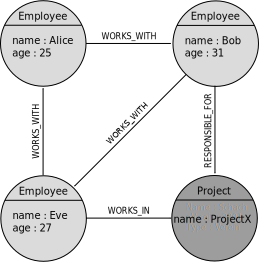
\includegraphics[scale=1]{neo4j_example.pdf}
	\caption[Neo4j: Beispielgraph]{Einfaches Beispiel eines Graphen mit den Knotenlabeln \texttt{Employee} und \texttt{Project} sowie den Kantenlabeln \texttt{WORKS\_WITH}, \texttt{WORKS\_IN} und \texttt{RESPONSIBLE\_FOR}.}
	\label{fig:neo4j_example}
\end{figure}

Abbildung \ref{fig:neo4j_example} zeigt einen schematisierten Beispielgraphen, welcher die Beziehungen zwischen Projekten und Mitarbeitern beschreibt. Knoten und Kanten besitzen entsprechende Label, Attribute werden ausschlie�lich an Knoten definiert. Cypher erm�glicht die Manipulation der Datenbasis: Unter Verwendung der \texttt{CREATE}-Klausel lassen sich Knoten- und Kanteninstanzen mit Labels und Properties erzeugen, mit der \texttt{SET}-Klausel Properties und Knotenlabel aktualisieren und die \texttt{DELETE}- bzw. \texttt{REMOVE}-Klausel erm�glicht das L�schen von Instanzen bzw. Properties. Mit der Anweisung

\texttt{CREATE (n:Employee \{name: \string"Alice\string", age: 25\})}

wird eine Knoteninstanz mit dem Label \texttt{Employee} und den Properties \texttt{name} und \texttt{age} erzeugt. Das Anlegen einer Kante erfordert das Vorhandensein der entsprechenden Knoten:

\texttt{MATCH a:Employee, b:Employee}\newline
\texttt{WHERE a.name = \string"Alice\string" AND b.name = \string"Bob\string"}\newline
\texttt{CREATE a-[r:WORKS\_WITH]->b}\newline
\texttt{RETURN r}

\texttt{MATCH}- und \texttt{WHERE}-Klausel dienen der Selektion von Objekten und werden nachfolgend im Zusammenhang mit lesenden Anfragen erl�utert. Die \texttt{CREATE}-Klausel erzeugt eine Kante von Alice nach Bob mit dem Label \texttt{WORKS\_WITH}. Die Richtung kann dabei durch die Verwendung von \texttt{<-} oder \texttt{->} angegeben werden, das Anf�gen von Kantenproperties ist in der Form \texttt{[r:WORKS\_WITH \{\string"since\string": 2010\}]} m�glich.

\paragraph*{Mustersuche via Cypher}

Eine rein lesende Anfrage setzt sich aus den folgenden Komponenten zusammen:

\texttt{[START] [MATCH] [WHERE]\newline
[WITH [ORDER BY] [SKIP] [LIMIT]]\newline
RETURN [ORDER BY] [SKIP] [LIMIT]}.

In der optionalen \texttt{START}-Klausel werden Bezeichner festgelegt und an Knoten- oder Kanteninstanzen gebunden. Die Auswahl einer Instanz erfolgt dabei entweder unter Angabe ihrer Identit�t oder mittels indexbasierter Suche. Zum Beispiel f�hrt die Anweisung 

\texttt{START a=node:Employees(name=\string"Alice\string")} 

zur Suche nach einem Knoten mit der Eigenschaft \texttt{name=\string"Alice\string"} innerhalb des Index\linebreak \texttt{Employees}, die Ergebnismenge wird an den Bezeichner \texttt{a} gebunden. Alle Bezeichner k�nnen in den nachfolgenden Teilen der Anfrage verwendet werden. Zul�ssige Datentypen f�r Bezeichner und Variablen sind generell Knoten, Kanten, Pfade und Literale bzw. deren Mengen.

\begin{figure}[h] 
	\centering
		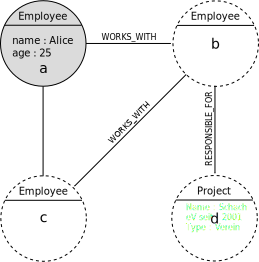
\includegraphics[scale=1]{neo4j_pattern.pdf}
	\caption[Neo4j: Mustergraph]{Beispiel f�r einen Mustergraphen: Der grau hinterlegte Knoten ist eine Konstante und stellt die Bindung zur Datenbasis her, wei� hinterlegte Knoten sind Variablen, welche w�hrend der Mustersuche gebunden werden.}
	\label{fig:neo4j_pattern}
\end{figure}

Wird keine \texttt{START}-Klausel definiert, ist die nachfolgende \texttt{MATCH}-Klausel obligatorisch. Sie erm�glicht die Definition eines Mustergraphen zum Auslesen von Informationen aus der Datenbasis. Ein Mustergraph besteht aus einer beliebigen Anzahl Variablen, welche beim Finden einer �bereinstimmung an Objektinstanzen gebunden werden. Mit dem Ziel, einen Mustergraphen in Textform zu repr�sentieren, wird dieser in Fragmente zerlegt, wobei jedes Fragment der Definition eines abstrakten Weges entspricht. Der in Abbildung \ref{fig:neo4j_pattern} gezeigte Mustergraph l�sst sich durch zwei Fragmente beschreiben:

\texttt{MATCH\newline
c:Employee---a-[:WORKS\_WITH]->b:Employee-[:WORKS\_WITH]->c, // 1\newline
b-[:RESPONSIBLE\_FOR]->d:Project // 2}

Innerhalb des Musters sind die in der \texttt{START}-Klausel definierten Bezeichner die Konstanten, sie stellen somit die Verbindungen zwischen Muster und Datenbasis her. Neo4j bezeichnet diese als \textit{bound pattern elements}, im Beispiel ist dies der Knoten \texttt{a}. Die Variablen \texttt{b}, \texttt{c} und \texttt{d} werden beim Finden einer �bereinstimmung an Knoten- bzw. Kanteninstanzen gebunden, alle Variablen stehen in den nachfolgenden Teilen der Anfrage zur Verf�gung. Am Beispiel wird die Verwendung der Knotenlabel deutlich: Die Variablen \texttt{b} und \texttt{c} legen das Label gebundener Knoteninstanzen auf \texttt{Employee} fest, w�hrend die Variable \texttt{d} die Menge m�glicher Instanzen auf Projekte einschr�nkt. Die Angabe eines Kantenlabels ist optional, so verlangt das erste Fragment im Beispiel eine Kante mit beliebiger Richtung und beliebigem Label zwischen den Knoten \texttt{c} und \texttt{a}, wohingegen zwischen den Knoten \texttt{b} und \texttt{d} eine gerichtete Kante mit dem Label \texttt{RESPONSIBLE\_FOR} existieren muss. Es besteht dar�ber hinaus die M�glichkeit, mehrere Kantenlabel zwischen zwei Knoten zu erlauben und einen Bereich f�r die L�nge des Weges zwischen den Knoten festzulegen. Dies erm�glicht das Finden von Pfaden beliebiger und fester L�nge und erlaubt eine hohe Flexibilit�t bei der Analyse von Beziehungsmustern. Der k�rzeste Pfad kann ebenfalls als Fragment eines Mustergraphen definiert werden. So bindet zum Beispiel der Ausdruck

\texttt{MATCH p = shortestPath(a:Employee-[*..5]-b:Project)}

die Variable \texttt{p} an die Instanz des k�rzesten Pfades zwischen Mitarbeiter \texttt{a} und Projekt \texttt{b}. Die L�nge des Pfades muss zwischen 0 und 5 betragen, Kantenlabel und -richtung  bleiben unber�cksichtigt. Alternativ liefert die Funktion \texttt{allShortestPaths} alle k�rzesten Pfade zwischen zwei Knoten.\\
Steht die \texttt{MATCH}-Klausel am Beginn der Anfrage, dann ist in diesem Abschnitt kein Bezeichner gebunden. Folglich wird entweder die vollst�ndige Datenbasis nach dem Muster durchsucht, oder anhand von eventuell definierten Labels die Menge der Objekte eingeschr�nkt. Alternativ k�nnen Pr�dikate in der nachfolgenden \texttt{WHERE}-Klausel zur Einschr�nkung des Suchraums genutzt werden.
	 
Die \texttt{WHERE}-Klausel entspricht der Selektion in der relationalen Algebra. Sie ist optional und erm�glicht die Filterung von Ergebnistupeln mittels Pr�dikaten. Cypher bietet eine Vielzahl mathematischer, vergleichender und boolescher Operatoren f�r die Definition und Verkn�pfung von Pr�dikaten an. Soll zum Beispiel im Mustergraphen das Attribut \texttt{age} der an die Variable \texttt{b} gebundenen Instanzen eingeschr�nkt werden, so ist dies mit folgender Anweisung m�glich:

\texttt{WHERE b.age > 23 AND b.age < 42}

Die ebenfalls optionale \texttt{WITH}-Klausel besitzt kein Pendant in der relationalen Algebra, sondern entspricht der Funktionsweise des Pipe-Operators der Linux-Shell. Mit dessen Hilfe lassen sich Operationen verketten: Die Ausgabe einer Operation kann als Eingabe der Folgeoperation verwendet werden. Dies ist in Cypher genau dann erforderlich, wenn Aggregate innerhalb einer \texttt{WHERE}-Bedingung verwendet werden sollen oder wenn lesende und schreibende Anfragen verkettet ausgef�hrt und die Sichtbarkeit der Variablen in Folgeoperationen gegeben sein muss.

Am Ende einer rein lesenden Cypher-Anfrage befindet sich die obligatorische \texttt{RETURN}-Klausel, diese entspricht der Projektion in der relationalen Algebra. Die Klausel legt fest, aus welchen Variablen sich das Anfrageergebnis zusammensetzt und erm�glicht die Umformung der gesamten Ergebnismenge bzw. einzelner Variablenwerte. Analog zu SQL kann das Ergebnis mit \texttt{ORDER BY} sortiert sowie durch \texttt{SKIP} und \texttt{LIMIT} eingeschr�nkt werden.

Cypher erm�glicht die Berechnung von Aggregaten sowohl in der \texttt{RETURN}- als auch in der \texttt{WITH}-Klausel, verschiedene Aggregatfunktionen, wie zum Beispiel \texttt{min}, \texttt{max} und \texttt{avg}, stehen zur Verf�gung. Dar�ber hinaus erm�glicht Cypher die Verwendung von skalaren (z.B. \texttt{LENGTH} und \texttt{TYPE}), mathematischen (z.B. \texttt{ABS} und \texttt{ROUND}), string-basierten (z.B. \texttt{SUBSTRING} und \texttt{LOWER}) und mengenorientierten (z.B. \texttt{FILTER} und \texttt{REDUCE}) Funktionen.

\texttt{MATCH}-, \texttt{WITH}- und \texttt{WHERE}-Klauseln lassen sich beliebig oft in beliebiger Reihenfolge kombinieren, so k�nnen zum Beispiel Ergebnismengen oder Aggregate in einer nachfolgenden Musterdefinition verwendet werden. Analog zum Traversal Framework werden rein lesende Anfragen erst ausgef�hrt, wenn der Nutzer auf die Ergebnisse zugreift, dies ist insbesondere dann sinnvoll, wenn ein Muster keine Bindung zur Datenbasis besitzt und diese folglich komplett durchsucht werden muss.

Die Sprache wird permanent weiterentwickelt, was bedeutet, dass mit �nderungen und Erweiterungen der Syntax zu rechnen ist. Schwerpunkt der Version 2.0 ist unter anderem die automatische Anfrageoptimierung. Eine manuelle Anfrageoptimierung ist m�glich, der Ausf�hrungsplan einer Cypher-Anfrage l�sst sich im eingebetteten Betrieb zusammen mit dem Anfrageergebnis abrufen und evaluieren.\\ Ein Vorteil gegen�ber den bisher vorgestellten Zugriffsm�glichkeiten ist der rein deklarative Charakter der Sprache. Im Gegensatz zur Core API wird in Cypher festgelegt was gesucht wird und nicht wie es gesucht wird. Dies erm�glicht eine abstrakte Anfrageformulierung und er�ffnet mehr M�glichkeiten zur systemseitigen Anfrageoptimierung. Demgegen�ber erm�glichen es Core API und Traversal Framework eigene Algorithmen zu implementieren und somit spezielle Anwendungsf�lle abzudecken. Die Aufgabe der Abstraktion erfordert dabei einen h�heren Entwicklungsaufwand und eine engere Kopplung der Implementierung an die Struktur der hinterlegten Daten. Dies erlaubt jedoch eine h�here Performance, da gezielt optimiert werden kann und die Schritte Anfrage�bersetzung und -optimierung entfallen.

\paragraph*{Transaktionen}

Alle Zugriffe auf die Datenbasis m�ssen innerhalb einer Transaktion erfolgen. Bei der Verwendung von Cypher erfolgt das Starten einer Transaktion implizit, ist bereits eine Transaktion im aktuellen Kontext aktiv, wird diese genutzt. Bei Verwendung der Core API m�ssen Transaktionen explizit gestartet werden. Nach einer Reihe von Lese- und Schreiboperationen wird die Transaktion entweder erfolgreich beendet (Commit) oder bei Eintritt eines Fehlers zur�ckgesetzt (Rollback). Um eventuell gehaltene Sperren freizugeben, muss die Transaktion grunds�tzlich finalisiert werden.\footnote{Dies orientert sich am \texttt{try-catch-finally}-Prinzip zur Behandlung von Ausnahmen in Java.}

In Neo4j werden flache Transaktionen unterst�tzt, welche sich im Quelltext jedoch auch beliebig schachteln lassen. Diese als \textit{Flat Nested Transactions} bezeichnete Umsetzung bedingt, dass ein Rollback einer untergeordneten Transaktion nicht isoliert, sondern nur �ber den Rollback der �bergeordneten Transaktion erfolgen kann. Dieser rekursive Ansatz hat bei Abbruch einer beliebigen untergeordneten Transaktion den Abbruch der Gesamttransaktion zur Folge.

Zur Vermeidung von Mehrbenutzeranomalien werden pessimistische RX-Sperrverfahren\footnote{Beim RX-Sperrverfahren werden zwei Arten von Sperren unterschieden: Lesesperren und exklusive Schreibsperren. Diese k�nnen auf einem Objekt gesetzt werden, um einen konkurrierenden Zugriff auszuschlie�en. Ist ein Objekt mit einer Lesesperre versehen, kann es von anderen Transaktionen gelesen, jedoch nicht geschrieben werden. Ist hingegen ein Objekt exklusiv gesperrt, so ist der lesende und schreibende Zugriff nur f�r den Sperrinhaber erlaubt, Lese- oder Schreibanforderungen anderer Transaktionen werden blockiert\cite{DBLP:books/sp/HarderR01}.} eingesetzt. Bei einem schreibenden Zugriff auf ein Objekt wird eine exklusive Sperre f�r das entsprechende Objekt gesetzt und bis zum Ende der Transaktion gehalten. Lesesperren hingegen werden nur f�r die Dauer des Lesevorgangs gehalten. Eine Transaktion sieht folglich nur eigene �nderungen und die �nderungen bereits beendeter Transaktionen. Entsprechend dem strikten Zwei-Phasen-Sperrprotokoll\footnote{Im Zwei-Phasen-Sperrprotokoll werden in einer Wachstumsphase zun�chst alle ben�tigten Sperren angefordert. Nachdem die erste Sperre wieder freigegeben wurde, d�rfen keine neuen Anforderungen erfolgen, es beginnt die Schrumpfungsphase in der Sperren nur noch freigegeben werden. Mit dem Ziel, Dirty Reads und kaskadierende R�cksetzungen infolge von Systemfehlern zu vermeiden, werden beim strikten Zwei-Phasen-Sperrprotokoll alle Sperren gleichzeitig freigegeben\cite{DBLP:books/sp/HarderR01}.} werden alle Schreibsperren am Ende der Transaktion gleichzeitig freigegeben.\\
Die langen Schreibsperren vermeiden das Problem der \textit{Dirty Reads}, durch die kurzen Lesesperren sind jedoch die Anomalien \textit{Non-Repeatable Read}, \textit{Phantom Problem} und vor allem auch \textit{Lost Update} m�glich. Dieser Zustand entspricht der Isolationsebene \texttt{READ COMMITTED}, sollen h�here Isolationsebenen wie zum Beispiel \texttt{REPEATABLE READ} oder\linebreak \texttt{SERIALIZABLE} erreicht werden, so liegt dies in der Verantwortung des Programmierers. Neo4j stellt Funktionen bereit, manuell Lese- bzw. Schreibsperren auf Knoten oder Kanten zu setzen.\\
Beim Einsatz exklusiver Sperren k�nnen wechselseitige Abh�ngigkeiten und somit Deadlocks entstehen. Neo4j begegnet diesem Problem mit Deadlock-Erkennung: Wird beim Anfordern einer exklusiven Sperre ein potentieller Deadlock erkannt, wird die anfordernde Transaktion zur�ckgesetzt.

�nderungen von Transaktionen erfolgen zun�chst ausschlie�lich im Hauptspeicher. Neo4j implementiert eine NoSteal-Strategie\cite{DBLP:books/sp/HarderR01}, bei der das Ausschreiben ge�nderter Objekte auf den Hintergrundspeicher vor dem Commit einer Transaktion nicht zul�ssig ist. Diese Strategie f�hrt dazu, dass nach einem Ausfall des GDBMS keine inkonsistenten �nderungen in der Datenbasis vorhanden sein k�nnen und somit keine UNDO-Informationen w�hrend der Transaktionsausf�hrung gespeichert werden m�ssen. Die Atomarit�t von Transaktionen wird durch dieses Vorgehen sichergestellt. Ein Nachteil dieser Strategie ist, dass sehr umfangreiche �nderungstransaktionen durch den verf�gbaren Hauptspeicher limitiert sind. Es kann erforderlich sein, diese in mehrere kleinere �nderungstransaktionen aufzuspalten.\\
Neben der Atomarit�t ist auch die Dauerhaftigkeit von �nderungen ein wesentliches Ziel von Transaktionen. Damit diese erreicht werden kann, f�hrt Neo4j ein Transaktions-Log, in dem alle �nderungen protokolliert werden. Beim erfolgreichen Beenden einer Transaktion wird ein Commit-Eintrag in die Log-Datei geschrieben, der dazu f�hrt, dass alle transienten �nderungen der Log-Datei auf dem Hintergrundspeicher persistiert werden. Beim Ausfall des GDBMS k�nnen somit alle bis dahin erfolgreich beendeten Transaktionen wiederhergestellt werden. Das Ausschreiben der �nderungen in die Datenbasis kann also verz�gert erfolgen. Dieses Vorgehen wird auch als NoForce-Strategie bezeichnet und verspricht gegen�ber dem unmittelbaren Ausschreiben beim Commit einen h�heren Durchsatz von Schreiboperationen\cite{DBLP:books/sp/HarderR01}.

Die Bewahrung der Konsistenz innerhalb der Datenbasis ist ebenfalls ein entscheidendes Kriterium bei der Ausf�hrung von Transaktionen. Die bereits erw�hnten modellinh�renten Integrit�tsbedingungen sind hierf�r ma�geblich verantwortlich.

\paragraph*{Indexverwaltung} F�r den performanten Zugriff auf Graphelemente anhand ihrer Properties unterst�tzt Neo4j die Definition von Indizes. Dies ist in Version 1.9 ausschlie�lich via Core API im eingebetteten und Client-Server-Betrieb m�glich. Ein Index wird entweder f�r Knoten oder f�r Kanten definiert und besitzt einen eindeutigen Bezeichner. Nach dem Erzeugen lassen sich Knoten- bzw. Kanteninstanzen unter Angabe eines beliebigen Schl�ssel-Wert-Paares in den Index einf�gen, dieser ist folglich nicht an ein konkretes Paar gebunden. Die Suche innerhalb eines Index erfolgt ebenfalls unter Angabe eines Schl�ssel-Wert-Paares, alle zugeh�rigen Instanzen werden zur�ckgegeben. Durch die fehlende Bindung an ein konkretes Property findet die Index-Aktualisierung bei �nderung der Datenbasis nicht automatisch statt: Nach dem Erzeugen bzw. L�schen einer Knoten- oder Kanteninstanz muss diese dem Index manuell hinzugef�gt bzw. entfernt werden. F�r das L�schen einzelner und mehrerer Eintr�ge sowie des gesamten Index stehen Funktionen zur Verf�gung. Eine automatische Indexierung wird ebenfalls angeboten: Hierf�r verwaltet das GDBMS je einen Index f�r Knoten und Kanten, welche unter Angabe einer Liste von Property-Schl�sseln systemseitig verwaltet werden.

Seit Version 2.0 unterst�tzt Neo4j zus�tzlich das Erzeugen von Schema-Indizes in Verbindung mit Knotenlabels. Dies ist sowohl in der Core API, als auch via Cypher m�glich. Der Cypher-Befehl

\texttt{CREATE INDEX ON :Employee(name)} 

erzeugt einen Index f�r alle Knoten mit dem Label \texttt{Employee} und indexiert zugeh�rige Instanzen anhand des Property-Schl�ssels \texttt{name}. Im Gegensatz zur bisherigen Umsetzung werden Schema-Indizes generell vom GDBMS verwaltet und automatisch aktualisiert, sobald sich die Datenbasis �ndert. Das L�schen eines Schema-Index ist weiterhin manuell m�glich.

Neo4j definiert eine Menge von Java-Schnittstellen mittels derer sich eigene Indexstrukturen implementieren lassen. Das GDBMS verwendet Apache Lucene\footnote{\url{http://lucene.apache.org/core/}} als Referenz-Implementierung, es handelt sich dabei um einen quelloffenen Volltext-Index zur Indizierung von Dokumenten auf der Grundlage von Termen. Eine weitere Implementierung ist zum Beispiel Neo4j-Spatial\footnote{\url{https://github.com/neo4j/spatial}}, eine Umsetzung des R-Baumes f�r r�umliche Anfragen. 

\subsection{Persistenz- und Cacheverwaltung}
\label{subsec:neo4j_persistency}

Neo4j ist ein natives GDBMS, was bedeutet, dass die physische Repr�sentation der Datenbasis f�r die graphenorientierte Verarbeitung optimiert ist. Mit dem Ziel indexfreie Adjazenz zu erreichen, wird die Datenbank auf mehrere Dateien, sog. Stores, aufgeteilt. Dabei soll durch die Trennung von Topologie und Nutzdaten das performante Traversieren des Graphen erm�glicht werden. Es existieren Stores f�r Knoten, Kanten, Properties und Knoten- bzw. Kantenlabels. Die Stores werden zusammen in einem benutzerdefinierten Verzeichnis gespeichert, das gleichzeitig die Identit�t der Datenbank darstellt.\\
Die Eintr�ge in den Stores, die nachfolgend als Satz bzw. Datensatz bezeichnet werden, besitzen ein festes Format und somit eine feste Satzl�nge. Dies hat den Vorteil, dass bei Angabe einer Identit�t, z.B. der Knoten-Identit�t 23, die Position des Knotens innerhalb des Stores durch Multiplikation mit der Satzl�nge in $\mathcal{O}(1)$ berechnet werden kann. Nachfolgend werden die Stores f�r Knoten, Kanten und Properties kurz beschrieben. Die zur Persistenz verf�gbare Dokumentation bezieht sich auf die stabile Version 1.9 des GDBMS, in dieser sind Knotenlabel nicht implementiert. Die folgenden Informationen stammen zum Teil aus dem Quelltext der Version 2.0.0-M04, dies wird an entsprechender Stelle kenntlich gemacht.

\begin{figure}[h] 
	\centering
		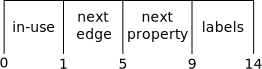
\includegraphics[scale=0.75]{neo4j_node_record.pdf}
	\caption[Neo4j: Datensatz eines Knotens]{Physische Repr�sentation eines Knotens in Neo4j. Der Datensatz hat eine feste L�nge von 14 Byte.}
	\label{fig:neo4j-node-record}
\end{figure}

In Abbildung \ref{fig:neo4j-node-record} wird der schematische Aufbau eines Datensatzes im Knoten-Store dargestellt, jeder Datensatz weist eine L�nge von 14 Byte auf.\footnote{Nachzuvollziehen unter \url{https://github.com/neo4j/neo4j/blob/2.0.0-M04/community/kernel/src/main/java/org/neo4j/kernel/impl/nioneo/store/NodeStore.java\#L68}.} Das erste Byte beinhaltet ein Flag, welches signalisiert, ob der entsprechende Knoten aktuell verwendet wird oder �berschrieben werden kann. Eine Liste freier Identit�ten wird in einer dedizierten Datei gef�hrt, beim L�schen eines Knotens wird dessen Identit�t der Liste hinzugef�gt und das Flag entsprechend gesetzt. Die folgenden vier Byte speichern die Identit�t der ersten Kante, die sich anschlie�enden vier Byte die Identit�t der ersten Property des Knotens. In den letzten f�nf Byte werden entweder die Label-Identit�ten des Knotens direkt gespeichert oder es wird auf eine Property verwiesen, welche die Knotenlabels beinhaltet. Das Format ist somit sehr leichtgewichtig und enth�lt fast ausschlie�lich Zeiger auf zugeh�rige Datens�tze.

\begin{figure}[h] 
	\centering
		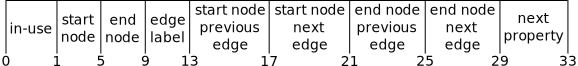
\includegraphics[scale=0.75]{neo4j_edge_record.pdf}
	\caption[Neo4j: Datensatz einer Kante]{Physische Repr�sentation einer Kante in Neo4j. Der Datensatz hat eine feste L�nge von 33 Byte.}
	\label{fig:neo4j-edge-record}
\end{figure}

Wie Abbildung \ref{fig:neo4j-edge-record} zu entnehmen ist, besitzt der Datensatz einer Kante im Vergleich zum Datensatz eines Knotens einen deutlich komplexeren Aufbau. Ziel ist es, ausgehend von einer Kante m�glichst effizient an weitere inzidente Kanten der Start- und Zielknoten zu gelangen. Zu diesem Zweck wird f�r beide Knoten je eine doppelt verkettete Liste inzidenter Kanten verwaltet. Jede Kante ist Element in zwei doppelt verketteten Listen und besitzt einen Verweis auf die vorhergehende und nachfolgende inzidente Kante des Start- bzw. Zielknotens. Durch die feste Satzl�nge im Kanten-Store ist das Berechnen der Position in $\mathcal{O}(1)$, das Traversieren der Nachbarschaft eines Knotens $v$ folglich in $\mathcal{O}(\left|N(v)\right|)$ m�glich. Das Einf�gen und L�schen in doppelt verketteten Listen erfolgt ebenfalls in $\mathcal{O}(1)$ \cite{ottmann2002algorithmen}.

Das Flag am Beginn eines Datensatzes hat den gleichen Zweck wie sein Pendant im bereits beschriebenen Knotenformat. In den sich anschlie�enden acht Byte werden die Identit�ten des Start- und Zielknotens gespeichert und so die Richtung der Kante festgelegt. Die n�chsten vier Byte beinhalten die Identit�t des Kantenlabels, welches in einem entsprechenden Store hinterlegt ist. In den nachfolgenden 16 Byte werden die Identit�ten adjazenter Kanten gespeichert. Der Verweis auf die erste Property befindet sich am Ende des Satzes. Durch die feste Satzl�nge in Label- und Property-Stores ist der Zugriff auf einzelne Elemente ebenfalls in konstanter Zeit m�glich, die Komplexit�t der Traversierung wird demnach nicht durch die Einschr�nkung auf bestimmte Labels oder Properties beeinflusst.

\begin{figure}[h]
	\centering	
	\subfigure[Vollst�ndiger Datensatz]{\label{fig:neo4j-property-record}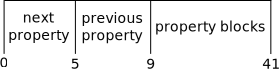
\includegraphics[scale=0.75]{neo4j_property_record.pdf}}\qquad	
	\subfigure[Einzelner Property-Block]{\label{fig:neo4j-property-block-record}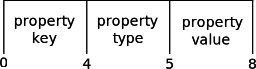
\includegraphics[scale=0.75]{neo4j_property_block_record.pdf}}	
	\caption[Neo4j: Datensatz einer Property]{Physische Repr�sentation von Properties in Neo4j. Der komplette Datensatz hat eine feste L�nge von 41 Byte, von denen 32 Byte f�r vier Property-Bl�cke zur Verf�gung stehen.}
\end{figure}

Knoten- und Kantenproperties werden ebenfalls in einer doppelt verketteten Liste verwaltet. Abbildung \ref{fig:neo4j-property-record} zeigt den schematischen Aufbau eines entsprechenden Datensatzes.\footnote{Nachzuvollziehen unter \url{https://github.com/neo4j/neo4j/blob/2.0.0-M04/community/kernel/src/main/java/org/neo4j/kernel/impl/nioneo/store/PropertyStore.java\#L57-L60}.} In den ersten neun Byte werden der vorhergehende und nachfolgende Datensatz referenziert. F�r Nutzdaten stehen insgesamt 32 Byte zur Verf�gung, diese werden in vier Bl�cke zu je acht Byte aufgeteilt. Jeder Block erm�glicht das Speichern einer Property und ist wie in Abbildung \ref{fig:neo4j-property-block-record} gezeigt aufgebaut: Die ersten vier Byte beinhalten einen Index-Schl�ssel, mit dessen Hilfe sich der Property-Schl�ssel aus einem Property-Index abrufen l�sst. Das n�chste Byte speichert den Typ des Property-Wertes, f�r den die �brigen drei Byte des Blocks reserviert sind. Reichen diese nicht aus, k�nnen bis zu drei weitere Bl�cke innerhalb des Datensatzes verwendet werden. Folglich lassen sich maximal vier Properties in einem Datensatz speichern. F�r gro�e Zeichenketten und Arrays werden spezielle dynamische Stores verwaltet, auf diese wird in den letzten drei Byte eines Blocks referenziert. Der erw�hnte Property-Index dient der Reduktion des Speicherbedarfs, da mehrfach verwendete Property-Schl�ssel nur einmal im Index gespeichert werden und ihr zugeh�riger Index-Schl�ssel in den Property-Bl�cken referenziert wird.
	
\paragraph*{Cacheverwaltung} Die Ausf�hrungen zeigen, dass sich die Position eines Datensatzes in konstanter Zeit berechnen l�sst. Der wahlfreie Zugriff auf Elemente innerhalb des Graphen bedingt jedoch auch den wahlfreien Zugriff auf die Stores und damit auf den langsamen Hintergrundspeicher. Wie f�r disk-zentrierte DBMS �blich, besitzt auch Neo4j Caches bzw. Puffer um einen m�glichst gro�en Teil der Datenbasis im Hauptspeicher vorzuhalten. In der Architektur werden zwei Caches unterschieden: Der Filesystem-Cache und der Object-Cache.

Der Filesystem-Cache beschleunigt sowohl Lese- als auch Schreibzugriffe. Jedem Store wird ein dedizierter Cache zugewiesen, dieser teilt den Store in eine feste Anzahl gleich gro�er Bereiche auf und h�lt m�glichst viele dieser Bereiche im Hauptspeicher. Die Cache-Gr��en k�nnen manuell konfiguriert werden, erfolgt dies nicht, orientiert sich die Gr��e am verf�gbaren Hauptspeicher, der JVM-Heap-Gr��e und der Gr��e der Stores. Als Ersetzungsverfahren wird Least Frequently Used (LFU) implementiert. Es handelt sich um ein Verfahren, welches jene Bereiche verdr�ngt, auf die im Vergleich zu anderen Bereichen seltener zugegriffen wird\cite{DBLP:books/sp/HarderR01}. F�r das Persistieren ausgelagerter Bereiche nutzt Neo4j standardm��ig Memory Mapped Files (MMF) des Betriebssystems und �berl�sst somit diesem die Entscheidung, welche Teile des virtuellen Speichers im Hauptspeicher gehalten und welche auf den Hintergrundspeicher geschrieben werden.

Das Instanziieren von Java-Objekten aus der physischen Repr�sentation kostet Zeit, h�ufig verwendete Objekte sollen demnach innerhalb des Object-Caches vorgehalten werden. Dieser soll insbesondere Lesezugriffe und das mit ihnen verbundene Traversieren beschleunigen. Alle Objekte innerhalb des Graphen werden beim ersten Zugriff instanziiert. Das bedeutet, dass zum Beispiel die inzidenten Kanten eines Knotens erst beim Abfragen der Nachbarschaft geladen und im Cache gruppiert nach Label und Richtung am Knoten abgelegt werden. Properties werden satzweise geladen, ausgelagerte Properties, wie lange Zeichenketten oder Arrays, erst beim direkten Zugriff. Der Object-Cache ben�tigt im Gegensatz zum Filesystem-Cache mehr Hauptspeicher f�r das Verwalten der gleichen Anzahl an Objekten.\footnote{Die Repr�sentation eines Knotens ohne Kanten und Properties als Java-Objekt ben�tigt zum Beispiel 344 Byte im Hauptspeicher. Der entsprechende Datensatz umfasst 14 Byte\cite{Neo4j_manual:2013}.} In der Community-Edition �berl�sst Neo4j der JVM die Verwaltung des Caches. Dies hat zwei wesentliche Nachteile, ein eingebettetes GDBMS teilt sich den verf�gbaren Speicher mit der Anwendung und der Garbage Collector der JVM entscheidet zu welchem Zeitpunkt Referenzen freigegeben werden. Letzteres erfolgt au�erhalb der Kontrolle des GDBMS und kann ggf. zu starken Leistungseinbr�chen f�hren. Die Enterprise-Edition beinhaltet eine eigene Cache-Implementierung mit fester Cache-Gr��e und manueller Objekt-Ersetzung, was mehr Kontrolle �ber die gepufferten Objekte erm�glicht.

\subsection{Verteilung und Skalierbarkeit}

Wie bereits erw�hnt, bietet Neo4j ausschlie�lich in der Enterprise Edition unter der Bezeichnung Neo4j High Availability (Neo4j HA) eine Verteilung der Datenbasis an. Die replizierte Datenverwaltung innerhalb des Rechner-Clusters erfolgt gem�� einer Master-Slave-Architektur\cite{rahm_masterslave}. Diese zeichnet sich dadurch aus, dass die Datenbasis im Sinne der vollst�ndigen Replikation auf allen Rechnern im Cluster gespeichert ist, Schreibzugriffe ausgehend von einem Master-Rechner koordiniert und �nderungen an mehrere Slave-Rechner weitergegeben werden. Die Architektur toleriert den Ausfall einzelner Rechner und gew�hrleistet eine horizontale Skalierbarkeit von Lesezugriffen. Die Funktionsweise wird nachfolgend anhand der internen Ausf�hrung von �nderungs- und Lesetransaktionen beschrieben.

Die Ausf�hrung von Schreibzugriffen im Rahmen von �nderungstransaktionen ist an allen Rechnern des Clusters m�glich. Erfolgt die Ausf�hrung an einem Slave, wird zur Vermeidung von Inkonsistenzen dessen Datenbasis zun�chst automatisch mit der des Masters synchronisiert. Der Commit einer Transaktion wird zuerst am Master und dann am Slave ausgef�hrt, anschlie�end wird der Client �ber den Erfolg bzw. Misserfolg der Ausf�hrung informiert. Dieses Vorgehen stellt sicher, dass die Daten nach erfolgreicher Beendigung einer Transaktion auf zwei Rechnern gespeichert sind. Erfolgt die Ausf�hrung hingegen direkt am Master, so ist der Ablauf zun�chst identisch zum nicht-verteilten Fall. Nach erfolgreicher Beendigung einer Transaktion wird der Client informiert und anschlie�end die �nderungen asynchron an eine definierte Anzahl Slaves repliziert (sog. Push-Prinzip).\footnote{Die Anzahl wird als \textit{Replication Factor} bezeichnet. Die Auswahl der Slaves kann statisch festgelegt werden oder nach dem Round-Robin-Prinzip erfolgen.} Die Replikation erfolgt optimistisch: Schl�gt das Abgleichen mit einem der Slaves fehl, ist die Transaktion dennoch erfolgreich. Das GDBMS stellt sicher, dass letztendlich alle Slaves synchronisiert werden, dieser Ansatz wird auch als \textit{Eventual Consistency}\cite{Vogels:2009:EC:1435417.1435432} bezeichnet.\footnote{Im Gegensatz zur \textit{Strong Consistency}, bei der nach Abschluss einer �nderungsoperation alle Instanzen im Cluster die gleiche Sicht auf die Daten haben, zeichnet sich die \textit{Weak Consistency} dadurch aus, dass selbst �nderungen an einer spezifischen Instanz bei einem nachfolgenden Lesezugriff an der gleichen Instanz nicht zwingend ber�cksichtigt werden. Die Eventual Consistency ist eine spezielle Form der Weak Consistency, bei der �nderungen an einer Instanz auch unmittelbar danach in Lesezugriffen ber�cksichtigt werden, jedoch nicht zwingend bei Lesezugriffen an anderen Instanzen\cite{Vogels:2009:EC:1435417.1435432}.}

Lesezugriffe k�nnen ebenfalls an allen Rechnern des Clusters durchgef�hrt werden. Aus den bisherigen Ausf�hrungen geht hervor, dass eine Situation m�glich ist, in der Slaves verschiedene Versionsst�nde in Bezug auf die Datenbasis aufweisen. Dies ist zum Beispiel genau dann der Fall, wenn der Replication Factor kleiner ist, als die Anzahl der Slaves im Cluster. Letztere werden synchronisiert, wenn sie eine �nderungstransaktion entgegennehmen oder, ausgehend vom Master, aktualisiert werden. Zus�tzlich l�sst sich ein Zeitintervall konfigurieren, in dem Slaves periodisch �nderungen vom Master beziehen (sog. Pull-Prinzip). Sollen �nderungen aus Anwendungssicht sofort wieder lesbar sein, so ist das Ausf�hren von �nderungs- und Lesetransaktionen am gleichen Slave erforderlich. Dieses Vorgehen resultiert jedoch im Allgemeinen in einer h�heren Antwortzeit, da Kommunikation zwischen Slave und Master stattfindet und die Daten synchron an beiden Rechnern geschrieben werden.
		
Jeder Teilnehmer im Cluster besitzt Funktionen zur Koordination bzw. Kommunikation mit dem Cluster. F�llt ein Rechner aus, wird dieser als tempor�r inaktiv gekennzeichnet. Handelt es sich um einen Slave, ist der Betrieb durch den Ausfall nicht beeintr�chtigt, nach der Reaktivierung wird der Rechner zun�chst mit dem Master synchronisiert und anschlie�end wieder in den Betrieb aufgenommen. F�llt jedoch der Master aus, muss aus den vorhandenen Slaves ein neuer Master gew�hlt werden. Neo4j implementiert hierf�r das Paxos-Protokoll\cite{hartung_paxos}, welches auf Basis eines Mehrheits-Votums den neuen Master bestimmt. �nderungstransaktionen, die w�hrend des Ausfalls aktiv sind, werden zur�ckgesetzt, neue �nderungstransaktionen werden solange blockiert, bis der neue Master aktiv ist. Datenverlust ist genau dann m�glich, wenn entweder der Master ausf�llt und die �nderungen noch nicht auf Slaves repliziert wurden oder wenn die �nderungstransaktion am Slave durchgef�hrt wird und anschlie�end Slave und Master gleichzeitig ausfallen. In beiden F�llen hat der neue Master folglich eine konsistente, jedoch veraltete Datenbasis.

\paragraph*{Skalierbarkeit} Die Architektur ist grunds�tzlich f�r die horizontale Skalierbarkeit von Lesezugriffen konzipiert. Der Skalierbarkeit sind jedoch auch Grenzen gesetzt, da ein einzelner Master f�r die Synchronisation aller Slaves verantwortlich ist. Schreibzugriffe skalieren generell nur vertikal, da jeder Schreibzugriff am Master ausgef�hrt werden muss und dieser im Cluster einmalig ist. Auch das maximale Datenvolumen ist begrenzt, da die vollst�ndige Datenbasis an jedem Rechner hinterlegt sein muss. Eine systemseitige Partitionierung der Datenbasis ist nicht implementiert. Neo Technology empfiehlt hier die anwendungsseitige Umsetzung unter Einbeziehung von Dom�nenwissen.
\section{HyperGraphDB}

HyperGraphDB ist ein quelloffenes GDBMS, das von Kobrix Software\footnote{\url{http://kobrix.com/index.jsp}} entwickelt wird. Die Quellcode-Lizenz ist GNU LGPL\footnote{Die Lizenz erlaubt die Verwendung in freier und kommerzieller Software. Die Verwendung in kommerzieller Software erfordert nicht, dass diese ebenfalls quelloffen sein muss: \url{http://www.gnu.org/licenses/lgpl-3.0.de.html}.}, die erste stabile Version 1.0 wurde 2010 ver�ffentlicht. Die Implementierung des Systems erfolgt ausschlie�lich in Java und sieht den Einsatz als eingebettetes Graphdatenbanksystem vor. Modellierung und Verwendung der Daten erfolgen graphenorientiert, Verarbeitung und Speicherung sind jedoch nicht-nativ: Der Graph wird auf eine Menge assoziativer Arrays abgebildet f�r deren Speicherung eine beliebige, entsprechend optimierte Speicherl�sung eingesetzt werden kann. Standardm��ig nutzt HyperGraphDB hierf�r die quelloffene, disk-orientierte Key-Value-Datenbank BerkeleyDB Java Edition\cite{Oracle_BerkeleyDB:2013}. Die Nutzung des Hauptspeichers als prim�res Speichermedium ist bei Verwendung einer entsprechenden Speicherschicht m�glich, HyperGraphDB bietet hierf�r jedoch keine Implementierung an. Das GDBMS kann als zentrales System oder in einer verteilten Konfiguration eingesetzt werden.

Grundlegend betrachtet handelt es sich um ein objektorientiertes Persistenz-Framework zur dauerhaften Speicherung von Java-Objektinstanzen. Die Repr�sentation der Daten im Hauptspeicher, Indexierung und Caching sind jedoch f�r die Unterst�tzung von Traversierung und Mustersuche ausgelegt. Wesentliche Eigenschaft des GDBMS und gleichzeitig Alleinstellungsmerkmal innerhalb der Evaluation ist die M�glichkeit zur Modellierung n-�rer Beziehungen: Als Datenmodell wird ein erweitertes Property-Hypergraph-Modell in Verbindung mit einem flexiblen Typsystem eingesetzt.\\
Konzipiert wurde das GDBMS f�r die Verwaltung hochkomplexer Daten, wie sie zum Beispiel in der Wissensverwaltung vorkommen\cite{Iordanov:2010:HGG:1927585.1927589}. Laut Hersteller eignet sich das System dar�ber hinaus f�r die Verwaltung sozialer Netzwerke und f�r den Einsatz in klassischen objektorientierten Gesch�ftsanwendungen\cite{HGDB_business_applications:2012}. Ein weiteres wichtiges Merkmal ist die offene Architektur, welche die Implementierung und Integration eigener Anfrage-,  Indizierungs-, Persistenz- und Verteilungsmechanismen erm�glicht.

Die nachfolgenden Ausf�hrungen beziehen sich auf Version 1.2 des GDBMS, diese wurde im November 2012 ver�ffentlicht. Der Gro�teil der Informationen stammt aus der offiziellen Dokumentation\cite{hypergraph_db_docu:2013} und der prim�ren Publikation zu HyperGraphDB\cite{Iordanov:2010:HGG:1927585.1927589}. Weitere Quellen werden an entsprechender Stelle genannt.

\subsection{Datenmodell und Typsystem}

% Modelltheorie
Die Basiseinheit zur Darstellung von Informationen innerhalb des Datenmodells ist das \textit{Atom}. Jedem Atom ist ein Tupel bestehend aus Atomen zugeordnet, dieses wird als \textit{Zielmenge} bezeichnet. Die Kardinalit�t der Zielmenge ist die \textit{Arit�t}: Ein Atom mit Arit�t Null ist ein Knoten, wohingegen ein Atom mit einer Arit�t gr��er Null eine Kante repr�sentiert.\footnote{Die Begriffe Kante und Hyperkante werden bei der Beschreibung von HyperGraphDB synonym verwendet.} Eine Kante kann folglich auf eine beliebige Anzahl von Atomen verweisen. Dies stellt eine Erweiterung des in Abschnitt \ref{subsec:hgm} definierten Hypergraph-Modells dar, da eine Kante in HyperGraphDB sowohl auf Knoten, als auch auf andere Kanten verweisen kann. Im Datenmodell werden Beziehungen zwischen Beziehungen als Relationen h�herer Ordnung bezeichnet. Die \textit{Inzidenzmenge} eines Atoms $a$ ist die Menge aller Atome, die $a$ in ihrer Zielmenge enthalten, d.h. die Menge aller gerichteter Kanten, die auf $a$ zeigen. An dieser Stelle wird deutlich, dass es sich um eine nicht-native Verarbeitung handelt, da ausgehend von einem Knoten nicht direkt auf dessen Nachbarschaft zugegriffen werden kann. Es muss zun�chst festgestellt werden, in welchen Zielmengen der entsprechende Knoten vorkommt. Wie nachfolgend gezeigt wird, setzt HyperGraphDB hierf�r entsprechende Indexstrukturen ein.

Neben der Zielmenge ist jedem Atom genau ein typisierter Wert zugeordnet. Der Typ ist beliebig und wird genau wie regul�re Daten innerhalb der Datenbasis als Atom gespeichert. Folglich k�nnen Beziehungen zwischen Typen untereinander bzw. zwischen Typen und ihren Instanzen abgebildet und in Operationen verwendet werden. Daraus geht hervor, dass Atome sowohl die Struktur als auch die Semantik des Graphen abbilden. Die Werte entsprechen den Nutzdaten und k�nnen beliebig strukturiert oder unstrukturiert sein und zur Laufzeit durch Werte eines anderen Typs ausgetauscht werden. Damit lassen sich Semantik und Struktur unabh�ngig voneinander �ndern, dies entspricht der Schemaevolution innerhalb einer Anwendung und bietet somit eine vergleichbare Flexibilit�t wie zum Beispiel Neo4j.

\paragraph*{Typsystem} Aus Anwendungssicht ist es die wesentliche Aufgabe eines Typen die Semantik der Daten zu beschreiben. Aus Systemsicht ist es hingegen die Serialisierung von Laufzeitobjekten in das Format der darunterliegenden Speicherschicht sowie die umgekehrte Deserialisierung. Im Sinne der Objektorientierung ist ein Typ somit eine abstrakte Fabrik und stellt Methoden zum Erzeugen, Speichern und L�schen von Laufzeitrepr�sentationen seiner Instanzen zur Verf�gung.\footnote{Das Aktualisieren eines Wertes ist nicht m�glich, da Werte in HyperGraphDB generell unver�nderlich (engl. \textit{immutable}) sind. Dies hat den Vorteil, dass ein Wert mehreren Atomen zugeordnet sein kann, f�hrt jedoch dazu, dass bei der Aktualisierung eines Wertes ein neuer Wert erzeugt werden muss.} Da es sich bei Typen um Atome handelt, besitzen auch diese einen �bergeordneten Datentyp. F�r jene, die bereits im Typsystem existieren, ist dies ein systemseitiger Datentyp mit der Bezeichnung \texttt{Top}. Wird hingegen ein Objekt, dessen Typ nicht bereits in der Datenbasis hinterlegt ist, zur Laufzeit eingef�gt, so ist dessen Typ ein Typkonstruktur. Dieser erzeugt neue aus bestehenden Typen, es handelt sich folglich um einen Datentyp, dessen Instanzen ebenfalls Datentypen sind.\\
Neben den genannten Operationen stellt ein Typ eine weitere Operation zur Verf�gung: Das Subsumieren. Eine Instanz A subsumiert eine Instanz B genau dann, wenn A allgemeiner ist als B bzw. wenn B immer dann verwendet werden kann, wenn A verwendet werden kann\cite{HGDB_subsume:2013}. Damit wird zum Beispiel gepr�ft, ob sich zwei Instanzen gegenseitig enthalten und folglich gleichwertig sind oder ob eine Instanz durch die andere ersetzt werden kann. Handelt es sich bei den Instanzen um Typen, so erm�glicht die Subsumierung die Abbildung von Vererbungshierarchien und somit die Konstruktion beliebiger Typsysteme: Wenn eine Instanz A eine zweite Instanz B subsumiert und A und B Typen sind, so erbt A von B.

Es sollte deutlich werden, dass ein Typ in HyperGraphDB ein Atom mit einer speziellen Rolle ist. Aus Anwendungssicht erm�glicht es die Definition von Knoten- und Kantenbezeichnern sowie das Speichern von Nutzdaten, aus Systemsicht die Verwaltung von Assoziationen sowohl zwischen einem Typ und seinen Instanzen als auch zwischen mehreren Typen. Das GDBMS beinhaltet vordefinierte Typimplementierungen f�r primitive Datentypen, JavaBeans\footnote{\url{http://www.oracle.com/technetwork/java/javase/documentation/spec-136004.html}}, 
Arrays, Collections, Maps und generell Klassen, welche die Schnittstelle \texttt{Serializable} implementieren.\footnote{Eine vollst�ndige �bersicht befindet sich im Quelltext des GDBMS unter \url{https://code.google.com/p/hypergraphdb/source/browse/tags/release1.2/core/src/config/org/hypergraphdb/types}} Vererbungshierarchien werden ebenfalls persistiert und durch einen dedizierten Kantentyp repr�sentiert. Sollen komplexere Datentypen verwendet werden oder ist die Einhaltung der JavaBeans-Spezifikation nicht m�glich, lassen sich eigene Datentypen implementieren. Diese werden im Typsystem des GDBMS registriert, anschlie�end lassen sich deren Instanzen in der Datenbasis verwalten.\\
Ein Typsystem erlaubt die Definition von Integrit�tsbedingungen und das GDBMS sorgt durch deren Einhaltung f�r die Wahrung der Konsistenz. So l�sst sich zum Beispiel die Zielmenge entsprechend typisierter Kanten auf definierte Typen einschr�nken, dar�ber hinaus ist das Definieren von Wertebereichen und Kardinalit�ten m�glich.

% eine oder mehrere Datenbanken
In HyperGraphDB existieren keine Prim�rschl�ssel, die Identit�t eines Atoms wird durch die Instanz eines sog. Handle repr�sentiert. Deren Funktion wird im Zusammenhang mit den Zugriffsmechanismen n�her erl�utert.

\subsection{Zugriffsmechanismen und Transaktionen}

HyperGraphDB bietet keine dedizierte Anfragesprache an, sondern erlaubt den Zugriff auf die Datenbasis ausschlie�lich via Java API im eingebetteten Betrieb. In diesem Zusammenhang stehen CRUD- und mengenorientierte Operationen sowie die M�glichkeit zur Traversierung des Graphen zur Verf�gung.

\paragraph*{CRUD-Operationen}

Das GDBMS bietet grundlegende Funktionen zum Erzeugen, Auslesen und L�schen von Atomen an. Da Werte innerhalb der Datenbasis unver�nderlich sind, erfolgt das Aktualisieren ausschlie�lich �ber den Austausch von Werten.

%Knoten
Ein Knoten definiert sich durch eine Objektinstanz innerhalb der Laufzeitumgebung. Diese l�sst sich dem Graphen hinzuf�gen: Ist ihr Datentyp bereits im Typsystem registriert, wird er automatisch mit dem Knoten verbunden, andernfalls zun�chst durch einen Typkonstruktor erzeugt. Das Resultat des Anlegens ist ein Handle, welches den Knoten innerhalb der Datenbasis identifiziert. Anhand des Handles kann die Objektinstanz und deren Typ aus der Datenbasis gelesen werden, umgekehrt l�sst sich unter Angabe der Objektinstanz das zugeh�rige Handle laden. Das L�schen eines Atoms ist ausschlie�lich unter Angabe des zugeh�rigen Handles m�glich.\\
In Verbindung mit dem flexiblen Typsystem und den vorhandenen Typimplementierungen lassen sich beliebige Nutzdaten an einem Knoten speichern. Wird zum Beispiel ein JavaBeans-Objekt dem Graphen hinzugef�gt, so wird dieses intern durch eine Record-Struktur repr�sentiert, die den schl�sselbasierten Zugriff auf die Attribute des Objektes erm�glicht. Da Attribute wiederum typisierte Werte sind, lassen sich beliebig verschachtelte Objekte hinterlegen.

%Kanten
Kanten werden in HyperGraphDB nicht durch Referenzen zwischen Objektinstanzen, sondern durch spezielle Kantenobjekte modelliert. Letztere sind Implementierungen der Schnittstelle \texttt{HGLink}, das GDBMS stellt drei Implementierungen zur Verf�gung: Kanten k�nnen ohne jegliche Zusatzinformationen, zum Beispiel ohne eine semantische Bedeutung oder ohne Nutzdaten, angelegt werden. Eine zweite Implementierung erlaubt das Speichern von Nutzdaten, dies k�nnen beliebig komplexe Objektinstanzen oder einfache Zeichenketten zur Festlegung eines Kantenbezeichners sein. Ein dritter Typ erm�glicht zudem das Festlegen zul�ssiger Typen innerhalb der Zielmenge und gestattet damit die Definition von Integrit�tsbedingungen.\\
Kanten werden unter Angabe ihrer Zielmenge und eventueller Nutzdaten erzeugt und anschlie�end mittels Handle identifiziert, Auslesen und L�schen erfolgen wie bereits f�r Knoten beschrieben. Kanten bieten dar�ber hinaus Funktionen zum Lesen der Zielmenge und der Arit�t an. Da die Zielmenge ein Tupel und somit geordnet ist, k�nnen Handles unter Angabe ihrer Position innerhalb der Zielmenge ausgelesen werden. Dies erm�glicht die Definition von Kantentypen die einzelnen Positionen innerhalb der Zielmenge eine Semantik zuordnen.

\paragraph*{Mengenorientierte Anfragen}

Neben dem Auslesen von Atomen unter Angabe ihres Handles bietet HyperGraphDB die M�glichkeit, deklarative, mengenorientierte Anfragen an die Datenbasis zu stellen. Die hierf�r vorhandene API basiert auf der Definition von Pr�dikaten zur Einschr�nkung der Ergebnismenge. Pr�dikate lassen sich konjunktiv bzw. disjunktiv verkn�pfen sowie beliebig schachteln und negieren. Sie beziehen sich entweder auf den Wert eines Atoms oder auf die Topologie des Graphen. Die folgende Anfrage definiert zum Beispiel die Menge aller Mitarbeiter, deren Attribut \texttt{age} kleiner oder gleich dem Wert 25 ist:

\texttt{hg.and(hg.type(Employee.class), hg.gte(\string"age\string", 25))}.

\texttt{hg} ist eine vom GDBMS bereitgestellte Klasse die syntaktisch verk�rzte, einfache Methoden f�r das Formulieren von Anfragen anbietet und diese intern auf eine komplexere API abbildet.\footnote{Die zugrundeliegende API wird an dieser Stelle nicht beschrieben, weil die Methoden der Klasse \texttt{hg} f�r die Erl�uterung ausreichend sind. Weiterf�hrende Informationen sind in der offiziellen Dokumentation enthalten\cite{hypergraph_db_docu:2013}.} In der Anfrage werden die Pr�dikate \texttt{hg.type(Employee.class)} und \texttt{hg.gte(\string"age\string", 25)} durch den logischen Operator \texttt{hg.and} konjunktiv verkn�pft. Das erste Pr�dikat legt den Typ des Atoms auf Mitarbeiter fest, w�hrend das zweite den Attributwert einschr�nkt. \texttt{Employee} ist im Beispiel eine Klasse nach JavaBeans-Spezifikation.

Neben den Werten l�sst sich auch die Topologie des Graphen in einer Anfrage durch Pr�dikate beschreiben. Das folgende Beispiel definiert die Menge aller Kanten, die zwei gegebene Atome in ihrer Zielmenge enthalten und insgesamt zehn Atome verbinden:

\texttt{hg.and(hg.link(atom1, atom2), hg.arity(10))}.

Im vorhergehenden Abschnitt wurde das Speichern eines Typs innerhalb der Datenbasis beschrieben: Vererbungshierarchien werden durch Subsumierung von Typen ausgedr�ckt, diese Beziehung l�sst sich folglich auch innerhalb von Anfragen verwenden. Nachfolgend wird die Menge aller Atome definiert, deren Datentyp von einer Klasse \texttt{Person} erbt und deren Instanzen nicht 25 Jahre alt sind:

\texttt{hg.and(hg.subsumes(Person.class), hg.not(hg.eq(\string"age\string", 25)))}.

Es handelt sich demnach um eine Anfrage, in der Topologie, Semantik und auch Nutzdaten des Graphen einbezogen werden. Neben den gezeigten stehen weitere Operatoren zum Vergleich von Werten, zur Einschr�nkung von Typbeziehungen und zur Beschreibung der Topologie zur Verf�gung.

F�r das Auslesen der Ergebnismenge werden drei Methoden angeboten: Grunds�tzlich wird ein Iterator erzeugt, mit dem sich die Ergebnismenge bi-direktional durchlaufen l�sst, der Wert eines Atoms wird erst beim Zugriff geladen. Die direkte Verwendung des Iterators bietet sich insbesondere bei umfangreichen Ergebnismengen an. Alternativ stellt die Klasse \texttt{hg} zwei Methoden zur Verf�gung, mit denen sich entweder die vollst�ndig deserialisierten Objektinstanzen oder nur deren Handles in einer Liste zur�ckgeben lassen.\\
Optional kann innerhalb einer Anfrage eine Abbildung definiert und mittels \texttt{hg.apply} auf die Ergebnismenge angewendet werden. Die Abbildung erm�glicht die Realisierung einer Projektion wenn nur bestimmte Attribute der Atomwerte ausgegeben werden sollen. Zus�tzlich kann eine Transformation der Elemente erfolgen. F�r eine Aggregation der Ergebnismenge stehen au�er \texttt{hg.count} keine Operatoren zur Verf�gung und m�ssen folglich bei Bedarf selbst implementiert werden.

An dieser Stelle sei auf die offene Architektur des GDBMS hingewiesen: Neue Operatoren lassen sich durch das Implementieren der Schnittstellen \texttt{HGAtomPredicate} und \texttt{HGQueryCondition} hinzuf�gen. Dies erlaubt das Definieren beliebiger dom�nenspezifischer Operatoren im Rahmen des beschriebenen Forschungsprojektes. Ein Beispiel hierf�r ist das Pr�fen, ob eine gegebene Kante eine kausale Abh�ngigkeit beschreibt. Dies ist genau dann der Fall, wenn alle in der Zielmenge vorhandenen Typen einen Datentyp zur Beschreibung transaktionaler Daten subsumieren.

\paragraph*{Traversierung}

Vergleichbar mit Neo4j steht in HyperGraphDB eine Menge von Schnittstellen zur Verf�gung, mit der sich eine Traversierung innerhalb der Datenbasis beschreiben l�sst. Die Reihenfolge, in der ein Graph durchlaufen wird, kann durch die Implementierung der Schnittstelle \texttt{HGTraversal} festgelegt werden. Es handelt sich um einen Iterator, dessen Elemente Paare von Handles sind. Jedes Paar besteht aus einer Kante und einem Atom, auf welches die Kante zeigt. Die Schnittstelle kann dar�ber hinaus pr�fen, ob ein Handle bereits w�hrend der Traversierung besucht wurde. HyperGraphDB stellt zwei Implementierungen der Schnittstelle zur Verf�gung: \texttt{HGBreadthFirstTraversal} f�r die Durchf�hrung eines Breitendurchlaufs und \texttt{HGDepthFirstTraversal} f�r die Durchf�hrung eines Tiefendurchlaufs. 

Neben dem Festlegen einer Reihenfolge kann es notwendig sein, die Menge der relevanten Paare einzuschr�nken. Hierf�r stellt HyperGraphDB die Schnittstelle \texttt{HGALGenerator} zur Verf�gung. Diese Schnittstelle erm�glicht es, eine Adjazenzliste (AL) zu generieren, welche jene Paare enth�lt, die ausgehend von einem Atom von der Traversierung ber�cksichtigt werden sollen. Auch hier stellt das GDBMS zwei Implementierungen zur Verf�gung. Der \texttt{SimpleALGenerator} erzeugt Adjazenzlisten aller benachbarter Atome ohne Ber�cksichtigung von Kanten- und Knotentypen bzw. deren Werten. Deutlich flexibler ist hingegen der \texttt{DefaultALGenerator}: Unter Verwendung der bereits beschriebenen Pr�dikate lassen sich sowohl Bedingungen f�r Kanten, als auch f�r Knoten\footnote{Semantisch korrekt w�re hier die Bezeichnung Geschwister, da eine Adjazenz auch zwischen Kanten definiert sein kann.} definieren. Das folgende kurze Beispiel verdeutlicht dies:

\texttt{DefaultALGenerator alGen = new DefaultALGenerator(graph,\newline
		hg.and(hg.type(WorksWith.class), hg.gte(\string"since\string", 2010)), // edge predicate \newline
		hg.and(hg.type(Person.class), hg.eq(\string"region\string", \string"Leipzig\string"))); // node predicate}
		
Es wird festgelegt, dass ausschlie�lich jene Kanten traversiert werden, die vom Typ \texttt{WorksWith} sind und deren repr�sentierte Beziehung seit 2010 besteht. Die Beziehung selbst soll nur zu Knoten bestehen, die vom Typ \texttt{Person} sind und aus der Region Leipzig stammen. Alle Unterklassen werden durch das Pr�dikat ebenfalls ber�cksichtigt.\\
Beide Implementierungen von \texttt{HGALGenerator} verbieten das mehrfache Besuchen von Knoten, d.h. wenn mehrere Paare bestehend aus unterschiedlichen Kanten und dem gleichen Knoten existieren, wird nur eines dieser Paare ber�cksichtigt. Letzteres kann durch eine eigene Implementierung umgangen werden. 

Sind Reihenfolge und eventuelle Einschr�nkungen definiert, wird die Traversierung unter Angabe eines Start-Handles initialisiert und gestartet. W�hrend der Ausf�hrung werden die relevanten Paare elementweise betrachtet. Dabei stehen im Gegensatz zu Neo4j keine Instanzen bereits berechneter Wege zur Verf�gung. Das Berechnen des aktuellen Abstands vom Startknoten oder das Speichern berechneter Wege muss bei Bedarf manuell erfolgen.\\
Zur Berechnung k�rzester Pfade steht eine Implementierung des Dijkstra-Algorithmus zur Verf�gung. Diese erfordert mindestens die Angabe eines Start- und eines Zielhandle. Dar�ber hinaus k�nnen optional ein \texttt{HGALGenerator} und nicht-negative Kantengewichte in Form eines assoziativen Arrays definiert werden. Soll der Ergebnispfad rekonstruierbar sein, so erfordert dies die �bergabe eines assoziativen Arrays: Dieses ordnet jedem Handle innerhalb des Pfades seinen jeweiligen Vorg�nger zu.

\paragraph*{Transaktionen}

% Zugriffsart, explizig, implizit

HyperGraphDB unterst�tzt die Ausf�hrung von Anfragen innerhalb von Transaktionen. F�r �nderungsoperationen ist dies obligatorisch, rein lesende Zugriffe k�nnen auch transaktionsunabh�ngig ausgef�hrt werden. Bei der Ausf�hrung einer einzelnen Schreiboperation wird eine Transaktion implizit erzeugt, sollen hingegen mehrere Zugriffe innerhalb einer Transaktion erfolgen, muss diese anwendungsseitig explizit erzeugt und verwaltet werden. Das GDBMS stellt hierf�r entsprechende Funktionen zur Verf�gung. Dar�ber hinaus besteht die M�glichkeit, Zugriffe an eine aktive Transaktion zu binden.\\ 
Transaktionen k�nnen beim Systemstart deaktiviert werden, dies ist zum Beispiel beim Importieren umfangreicher Datenmengen sinnvoll und setzt voraus, dass keine nebenl�ufigen Zugriffe erfolgen. Bez�glich der ACID-Eigenschaften sind Transaktionen in HyperGraphDB atomar, konsistent und erfolgen isoliert voneinander. Die Dauerhaftigkeit wird nicht garantiert, was bedeutet, dass �nderungen erfolgreich beendeter Transaktionen nach einem Systemfehler verloren sein k�nnen. Der Hersteller begr�ndet dies mit dem daraus resultierenden h�heren Schreibdurchsatz und mit der geringen H�ufigkeit kompletter Abst�rze der JVM.

% Schachtelung von Transaktionen

Das GDBMS erlaubt die Schachtelung von Transaktionen: Im Gegensatz zu Neo4j lassen sich dabei untergeordnete Transaktionen isoliert zur�cksetzen. Der Abbruch einer �bergeordneten Transaktionen f�hrt zum Rollback aller ihr untergeordneten Transaktionen. Dies hat zur Folge, dass ein Fehler in komplexen, lange laufenden Transaktionen isoliert behandelt und der Arbeitsverlust je nach Granularit�t der Aufteilung minimiert werden kann.

% Mehrbenutzeranomalien

Wie bereits erw�hnt, nutzt HyperGraphDB die Key-Value-Datenbank BerkeleyDB f�r die Speicherung der Datenbasis. Diese verwendet ein pessimistisches RX-Sperrverfahren zur Vermeidung von Lese-Schreib-Konflikten. In BerkeleyDB lassen sich verschiedene Isolationsebenen konfigurieren, standardm��ig wird \texttt{REPEATABLE READ} verwendet\cite{oracle:2013}. Lese- und Schreibsperren werden in dieser Stufe f�r die Dauer der gesamten Transaktion gehalten. Somit werden die Mehrbenutzeranomalien Dirty Read, Non-Repeatable Read und Lost Update vermieden. Das Phantom Problem beim parallelen Einf�gen neuer Datens�tze ist weiterhin m�glich.\\
% Deadlocks
BerkeleyDB implementiert einen Timeout-Mechanismus\cite{DBLP:books/sp/HarderR01} zur Erkennung von\linebreak~Deadlocks\cite{oracle:2013}. Der Timeout legt fest, wie lange eine Sperre auf einem Objekt gehalten werden kann. Wird dieser Wert �berschritten, geht das System von einem Deadlock aus. Da dies nicht zwingend der Realit�t entsprechen muss, sollte der Wert dem Zugriffsverhalten und der erwarteten Transaktionsdauer entsprechend angepasst werden um unn�tige R�cksetzungen zu vermeiden. Wird ein potentieller Deadlock erkannt, benachrichtigt BerkeleyDB die Anwendung, d.h. HyperGraphDB, mittels einer Ausnahme. Die Behandlung dieser Ausnahme wird entweder von HyperGraphDB oder von Anwendung �bernommen: Das GDBMS bietet die M�glichkeit eine in Folge eines Deadlocks abgebrochene Transaktion automatisch zu wiederholen bis diese erfolgreich beendet wird. Alternativ wird die Ausnahme an die Anwendung weitergeleitet, welche �ber die nachfolgenden Schritte individuell entscheidet.

% Logging

HyperGraphDB garantiert standardm��ig keine Dauerhaftigkeit von Transaktionen. Um dies zu erl�utern,  muss kurz auf die Interna von BerkeleyDB eingegangen werden: BerkeleyDB bildet eine Datenbank innerhalb eines B-Baumes ab. Es handelt sich um eine spezielle Form, in der Nutzdaten ausschlie�lich in den Bl�ttern hinterlegt sind. �nderungsoperationen beeinflussen sowohl die Struktur des Baumes als auch die Eintr�ge in den Bl�ttern. Zur Gew�hrleistung von Dauerhaftigkeit nutzt BerkeleyDB ein Transaktions-Log, in dem alle logischen �nderungsoperationen registriert werden. Dies bedeutet, dass sich durch sequentielles Ausf�hren der Log-Eintr�ge der B-Baum rekonstruieren l�sst. Folglich ist das Transaktions-Log die Datenbasis. Um den Wiederherstellungsaufwand im Fehlerfall zu minimieren, werden periodisch Sicherungspunkte geschrieben in denen der B-Baum vollst�ndig gespeichert ist\cite{oracle_bdb:2013}.\\
Das Transaktions-Log wird permanent im Hauptspeicher gehalten. Kommt es w�hrend der Ausf�hrung einer Transaktion zum Ausfall des GDBMS, sind die bis dahin erfolgten �nderungen ausschlie�lich im Hauptspeicher und somit verloren. Die Atomarit�t einer Transaktion ist damit sichergestellt und eine UNDO-Recovery nicht erforderlich. F�r die Wiederholbarkeit erfolgreicher Transaktionen wird beim Commit  ein entsprechender Eintrag in das Log geschrieben. In der Standardeinstellung von BerkeleyDB f�hrt dieser Eintrag zum Ausschreiben des Logs auf den Hintergrundspeicher, eine REDO-Recovery ist folglich m�glich. HyperGraphDB initialisiert BerkeleyDB standardm��ig mit einer Konfiguration, die es der Datenbank erlaubt, das Transaktions-Log asynchron auf den Hintergrundspeicher zu schreiben, was bedeutet, dass �nderungen zum Commit-Zeitpunkt nicht unmittelbar persistiert werden.\footnote{Die Initialisierung kann im Quelltext unter \url{https://code.google.com/p/hypergraphdb/source/browse/tags/release1.2/storage/bdb-je/src/java/org/hypergraphdb/storage/bje/BJEConfig.java} in Zeile 64 nachvollzogen werden} Kommt es zwischen Commit und Persistieren des Logs zum Systemausfall, sind die �nderungen der Transaktion verloren.

\subsection{Persistenz-, Index- und Cacheverwaltung}

Wie anfangs erw�hnt, ist HyperGraphDB ein nicht-natives GDBMS, welches den Graphen auf assoziative Arrays abbildet und diese im Rahmen der Anfrageausf�hrung und der physischen Repr�sentation der Datenbasis verwendet. Die Organisation erfolgt dabei innerhalb des GDBMS in zwei Schichten: Der primitiven Speicherschicht, welche direkt auf das eingesetzte Speichersystem zugreift, und der Modellschicht, welche von der primitiven Speicherschicht abstrahiert und die darin enthaltenen Informationen als Elemente des Datenmodells darstellt. Das eingesetzte Speichersystem wird nachfolgend als physische Speicherschicht bezeichnet, da es letztendlich die Persistenz der Daten sicherstellt, standardm��ig ist dies BerkeleyDB Java Edition.

Die primitive Speicherschicht repr�sentiert einen Graphen bestehend aus Identit�ten und ihnen zugeordneter Rohdaten, eine semantische Zuordnung findet in dieser Schicht nicht statt. F�r die Speicherung werden zwei assoziative Arrays verwendet:

\texttt{LinkStore: ID $\rightarrow$ List<ID>}\newline
\texttt{DataStore: ID $\rightarrow$ byte[]}

Der \texttt{LinkStore} bildet die Topologie des Graphen ab, indem er Identit�ten (IDs) eine Liste weiterer Identit�ten zuordnet. Im \texttt{DataStore} werden einer Identit�t Rohdaten in Form eines Byte-Arrays zugewiesen. Jeder Datensatz in der primitiven Speicherschicht ist folglich ein Schl�ssel-Wert-Paar. Der Schl�ssel wird in HyperGraphDB durch ein spezielles Handle repr�sentiert, das sog. \texttt{HGPersistentHandle}. Dieses ordnet jeder Entit�t eine UUID fester L�nge zu. Innerhalb der primitiven Speicherschicht ist somit der \texttt{LinkStore} eine Liste von Instanzen des genannten Handles.

Die Modellschicht wandelt die Informationen der primitiven Speicherschicht in die abstrakten Elemente des Datenmodells um. Nachfolgend sind alle ID-Bezeichner als Instanzen von \texttt{HGPersistentHandle} zu verstehen. 

\texttt{AtomID $\rightarrow$ [TypeID, ValueID, TargetID, ..., TargetID]}\newline
\texttt{ValueID $\rightarrow$ [ID, ID, ..., ID] | byte[]}\newline
\texttt{TypeID $\rightarrow$ AtomID}\newline
\texttt{TargetID $\rightarrow$ AtomID}

Ein Eintrag im \texttt{LinkStore} wird in der Modellschicht entweder als Atom oder als Wert eines zusammengesetzten, nicht-primitiven Datentyps interpretiert. Im ersten Fall verweist die \texttt{TypeID} auf den Typ des Atoms w�hrend die \texttt{ValueID} den zugeh�rigen Wert referenziert. Anschlie�end wird die Zielmenge des Atoms aus einer Menge von \texttt{TargetIDs} definiert. Da ein Knoten im Datenmodell ein Atom mit Arit�t Null ist, enth�lt seine physische Repr�sentation im Gegensatz zu einer Kante nur den Verweis auf seinen Typ und den Wert. Da sowohl der Typ eines Atoms als auch die Eintr�ge in der Zielmenge Atome sind, referenzieren \texttt{TypeID} und \texttt{TargetID} eine \texttt{AtomID}.\\
Alternativ repr�sentiert ein Eintrag im \texttt{LinkStore} den Wert eines zusammengesetzten, nicht-primitiven Datentyps und wird mittels \texttt{ValueID} referenziert. Wird hingegen nur der Wert eines primitiven Datentyps am Atom gespeichert verweist die \texttt{ValueID} direkt auf das entsprechende Byte-Array im \texttt{DataStore}. An dieser Stelle wird deutlich, warum Werte an Atomen grunds�tzlich unver�nderlich sind und eine Wert�nderung nur durch den Austausch des Wertes erfolgen kann.\\
Die Deserialisierung der Werte erfolgt nicht in der Modellschicht, sondern wird von der jeweiligen Typimplementierung bzw. vom jeweiligen Typkonstruktur durchgef�hrt. Im Zusammenhang mit dem Typsystem wurde bereits erw�hnt, dass Typen abstrakte Fabriken sind und unter anderem eine Methode zum Erzeugen der entsprechenden Instanzen zur Verf�gung stellen. Diese Methode nimmt die \texttt{ValueID} entgegen und f�hrt die Deserialisierung durch.\footnote{Dies l�sst sich im Quelltext des \texttt{HGAtomType} nachvollziehen: \url{https://code.google.com/p/hypergraphdb/source/browse/tags/release1.2/core/src/java/org/hypergraphdb/type/HGAtomType.java}, Zeile 65.}

In der physischen Speicherschicht (BerkeleyDB) werden die Werte von \texttt{LinkStore} und \texttt{DataStore} als Byte-Arrays abgelegt. Die Deserialisierung der Identit�ten erfolgt in der primitiven Speicherschicht, erm�glicht wird dies durch die feste L�nge der UUIDs. Die Byte-Arrays im \texttt{DataStore} k�nnen erst in der Modellschicht deserialisiert werden, da erst hier Informationen zum Datentyp vorhanden sind. Es sollte deutlich werden, dass sich die Schl�sselmengen von \texttt{LinkStore} und \texttt{DataStore} �berlappen k�nnen und diese somit in zwei getrennten Key-Value-Datenbanken gespeichert werden m�ssen.

% Index

\paragraph*{Indexverwaltung}

F�r die effiziente Ausf�hrung mengenorientierter und traversierender Anfragen beinhaltet die Modellschicht drei zus�tzliche Indexstrukturen, welche jeweils in einer Key-Value-Datenbank der physischen Speicherschicht persistiert werden:

\texttt{IncidenceIndex: UUID $\rightarrow$ SortedSet<UUID>}\newline
\texttt{TypeIndex: UUID $\rightarrow$ SortedSet<UUID>}\newline
\texttt{ValueIndex: UUID $\rightarrow$ SortedSet<UUID>}

Der \texttt{IncidenceIndex} ordnet jedem Atom seine Inzidenzmenge zu, d.h. die Menge aller Kanten die auf das Atom zeigen. Der \texttt{TypeIndex} verweist auf die Menge aller Instanzen eines gegebenen Datentyps und der \texttt{ValueIndex} weist einem Wert die Menge der Atome zu, die ihn besitzen. Bei zusammengesetzten Werten wird der Wert auf h�chster Ebene indexiert. Zu beachten ist, dass die zugeordneten Werte geordnete Mengen sind auf denen sich Mengenoperationen effizient ausf�hren lassen. Folglich lassen sich mit Hilfe der Indexstrukturen graphenspezifische Operationen effizient ausf�hren. Zum Beispiel l�sst sich anhand der Schnittmenge der Inzidenzlisten zweier Knoten pr�fen, ob diese adjazent sind.

Neben den systemseitigen Indexstrukturen k�nnen auch von der Anwendung zus�tzliche Indizes definiert werden. Mit diesen ist das Indexieren sowohl der Topologie des Graphen als auch der hinterlegten Nutzdaten m�glich. Indizes sind immer an einen Typ gebunden, gelten jedoch f�r alle Typen, welche diesen subsumieren. Auch im Zusammenhang mit Indexstrukturen wird die offene Architektur des GDBMS deutlich: Das Implementieren der Schnittstelle \texttt{HGIndexer} erm�glicht das Hinzuf�gen eigener Datenstrukturen. HyperGraphDB beinhaltet bereits Implementierungen zur Indexierung der Attribute eines Datentyps oder zur Indexierung vollst�ndiger Werte eines Atoms. F�r den effizienten Zugriff auf Teilgraphen erm�glicht eine weitere Implementierung die Indexierung der kompletten Zielmenge eines Atoms. Ein weiterer topologischer Index indexiert Kanten anhand eines Atoms an einer expliziten Position innerhalb der Zielmenge. Wie bereits erw�hnt, ist diese geordnet, die Positionen k�nnen somit anwendungsseitig mit einer Semantik versehen werden.

Aus den bisherigen Ausf�hrungen geht hervor, dass HyperGraphDB mindestens f�nf Key-Value-Datenbanken zur Abbildung der primitiven Speicherschicht und der obligatorischen Indexstrukturen einsetzt. F�r jeden anwendungsseitig definierten Index wird eine zus�tzliche Datenbank ben�tigt. Die Komplexit�t der einzelnen Operationen ist dabei im Wesentlichen von der Implementierung des Speichersystems abh�ngig. Wie bereits im Zusammenhang mit Transaktionen beschrieben, speichert BerkeleyDB die Daten einer Datenbank in den Bl�ttern eines B-Baumes. Der Zugriff auf diese Daten ist somit logarithmisch von der Anzahl der Eintr�ge und der Ordnung des Baumes abh�ngig\cite{ottmann2002algorithmen}. Die indexfreie Adjazenz ist hingegen nur m�glich, wenn sich die Daten in konstanter Zeit lesen lassen. BerkeleyDB verf�gt �ber Caches um den Zugriff auf die Datenbasis zu beschleunigen\cite{oracle_bdb:2013}. Da es sich jedoch um ein austauschbares Speichersystem handelt, wird nachfolgend nur die Cacheverwaltung von HyperGraphDB beschrieben.

% Caching

\paragraph*{Cacheverwaltung}

F�r den performanten, wahlfreien Zugriff auf die Elemente innerhalb des Graphen bietet auch HyperGraphDB Caches an: Den Atom-Cache und einen Cache f�r Inzidenzmengen. Der Atom-Cache erm�glicht den effizienten Zugriff sowohl auf die Objektinstanz unter Angabe des zugeh�rigen Handles als auch f�r den umgekehrten Fall. Realisiert wird der Cache durch zwei Hashtabellen und die Verwendung schwacher Referenzen. Letztere zeichnen sich dadurch aus, dass sich die von ihnen referenzierten Objektinstanzen vom Garbage Collector aus dem Speicher verdr�ngen lassen\cite{oracle_weak_references:2013}, beim Zugriff auf die Referenz wird das Objekt wiederhergestellt. Ein Atom wird folglich genau dann aus dem Cache verdr�ngt, wenn es entweder manuell durch die Anwendung oder automatisch durch die JVM entfernt wird.\\
Der zweite Cache beschleunigt den Zugriff auf die Inzidenzmengen der Atome und wird ebenfalls durch eine Hashtabelle realisiert. Hierf�r implementiert HyperGraphDB einen Least Recently Used Cache (LRU), welcher jene Objekte vorh�lt, auf die als letztes zugegriffen wurde. Bei der Instanziierung kann festgelegt werden, welcher Anteil des freien Speichers vom Cache genutzt werden darf und wie gro� der Anteil zu verdr�ngender Elemente bei �berschreiten der Speichergrenze sein soll.

% Cache Synchronisation
Alle Transaktionen in HyperGraphDB greifen auf den Atom-Cache zu, die ACID-\linebreak~Eigenschaften m�ssen somit auch bei der Verwendung des Caches gegeben sein. Das in diesem Zusammenhang eingesetzte Verfahren ist Multiversion Concurrency Control (MVCC), ein optimistisches Synchronisationsverfahren f�r nebenl�ufige Transaktionen\cite{DBLP:books/sp/HarderR01}.\footnote{Das Verfahren verzichtet auf das Setzen von Lese- und Schreibsperren, stattdessen werden zu �ndernde Objekte dupliziert und �nderungen an den Duplikaten durchgef�hrt. Objektduplikate werden durch das F�hren einer Versionsnummer unterschieden. Leseoperationen greifen ausschlie�lich auf jene Objektversionen zu, die zum Beginn der Transaktion aktuell waren und erhalten folglich immer eine konsistente Sicht auf die Datenbasis.\footnote{Dies entspricht dem Konzept der reihenfolgeerhaltenden Serialisierbarkeit\cite{DBLP:books/sp/HarderR01}.} Reine Lesetransaktionen k�nnen somit ohne Blockierungen durchgef�hrt werden. �nderungstransaktionen werden erst beim Commit auf eventuell vorhandene Konflikte mit nebenl�ufigen Transaktionen �berpr�ft. Dies erfolgt �ber den Vergleich von Versionsnummern der ge�nderten Objekte: Stimmt die Versionsnummer des Objektes zum Commit-Zeitpunkt mit der Versionsnummer bei der Duplikaterstellung �berein, liegt kein Konflikt vor. Sind die Versionen hingegen verschieden, hat eine nebenl�ufige Transaktion das Objekt und somit die Versionsnummer ge�ndert, die aktuelle Transaktion muss folglich zur�ckgesetzt werden. Ist hingegen die beschriebene �bereinstimmung der Versionen f�r alle ge�nderten Objekte gegeben, so ist die Transaktion valide und ihre �nderungen k�nnen im Cache sichtbar gemacht werden.} In diesem Konzept sind keine Mehrbenutzeranomalien m�glich, die Isolationsebene innerhalb des Caches ist somit \texttt{SERIALIZABLE}. In Verbindung mit der Transaktionsausf�hrung in der physischen Speicherschicht l�sst sich der Ablauf beim Commit einer Transaktion in HyperGraphDB anhand der folgenden Schritte zusammenfassen:

\begin{enumerate}
	\item Anfordern einer Commit-Sperre um nebenl�ufige Commits zu blockieren
	\item Pr�fen, ob die Transaktion im Cache valide ist
	\item Ausf�hrung des Commit in der physischen Speicherschicht (BerkeleyDB)
	\item Schreiben der �nderungen im Cache
	\item Freigabe der Commit-Sperre
\end{enumerate}

Ist die Transaktion bereits im Cache nicht valide oder f�hrt das Commit in der physischen Speicherschicht zum Abbruch der Transaktion, werden die �nderungen im Cache verworfen und die Transaktion ist zur�ckgesetzt.\footnote{Die Erl�uterung der Transaktionsverwaltung innerhalb des Caches ist nicht Teil der offiziellen Dokumentation, sondern basiert auf der Recherche innerhalb des Quelltextes von HyperGraphDB. Die dabei dokumentierten internen Abl�ufe wurden im Austausch mit dem Entwickler best�tigt: \url{https://groups.google.com/forum/?hl=de\#!topic/hypergraphdb/fmjdVtDxf-g.}} F�r die Verwaltung der Duplikate nutzt HyperGraphDB Versioned Boxes\cite{Cachopo:2006:VBB:1228561.1228566}, das Vermitteln der Funktionsweise �berschreitet jedoch den Rahmen der vorliegenden Evaluation und ist f�r das Verst�ndnis der Transaktions- und Cacheverwaltung nicht erforderlich.

\subsection{Verteilung und Skalierbarkeit}

Die Verteilung der Datenbasis erfolgt in HyperGraphDB unter Verwendung eines integrierten Peer-to-Peer-Frameworks, welches verschiedene Mechanismen zur Kommunikation zwischen verteilten Datenbankinstanzen bereitstellt. Eine Peer-to-Peer-Kommunikation zeichnet sich im Gegensatz zur Client-Server-Kommunikation dadurch aus, dass alle Teilnehmer gleichberechtigt sind und innerhalb des Netzes keine zentrale Instanz existiert\cite{Tanenbaum:2002:CN:572404}. F�r die Kommunikation zwischen den Peers setzt HyperGraphDB die standardisierte Agent Communication Language\footnote{\url{http://www.fipa.org/repository/aclspecs.html}} ein, die �bertragung erfolgt in Form von Nachrichten auf Grundlage des XMPP-Protokolls\footnote{\url{http://xmpp.org/xmpp-protocols/rfcs/}}. Die Kommunikation selbst ist  asynchron, was bedeutet, dass Nachrichten von Peers empfangen, in einem Pool gesammelt und anschlie�end in beliebiger Reihenfolge verarbeitet werden.

Intention von HyperGraphDB ist das Definieren einer Datenverteilung innerhalb der Anwendung, da diese unter Ber�cksichtigung von Dom�nenwissen besser entscheiden kann, wie die Daten zu partitionieren bzw. zu replizieren sind. Das Framework ist somit ausschlie�lich als Mittel zur Umsetzung konkreter Verteilungsalgorithmen gedacht. Auf eine detaillierte Beschreibung des Frameworks wird an dieser Stelle verzichtet, da dies nicht dem Schwerpunkt der Evaluation entspricht. Sollte HyperGraphDB f�r das Forschungsprojekt eingesetzt und dabei eine Verteilung realisiert werden, so findet sich eine ausf�hrliche Beschreibung des Frameworks in der offiziellen Dokumentation.

In \cite{Iordanov:2010:HGG:1927585.1927589} wird ein sehr abstraktes Beispiel f�r die Umsetzung einer Replikation in HyperGraphDB vorgestellt. Auf dieser Grundlage wird nachfolgend - stark vereinfacht -  die m�gliche Realisierung einer fragmentierten Replikation beschrieben: Ein Peer kann durch die Definition von Pr�dikaten die f�r ihn interessanten Atome festlegen. Zum Beispiel kann durch die Verwendung von Typ-Pr�dikaten bestimmt werden, welcher Peer die Instanzen eines Typs speichert. Folglich l�sst sich durch Partitionierung des Schemas festlegen, welche Atome zusammen gespeichert sind. Die Anzahl der Peers, die das gleiche Typ-Pr�dikat besitzen, entspricht der Anzahl der Replikate der jeweiligen Instanzen. Die Pr�dikate aller Peers sind jedem Teilnehmer innerhalb des Netzwerkes bekannt. Sobald ein Atom ein definiertes Pr�dikat erf�llt, werden alle daran interessierten Peers benachrichtigt. Die Pr�fung erfolgt event-basiert beim Erzeugen, L�schen oder Aktualisieren eines Atoms innerhalb einer Transaktion. Die Nachricht selbst beinhaltet die zugeh�rige Transaktion. Trifft die Nachricht beim Interessent ein, best�tigt er diese und entscheidet selbst, ob er die Transaktion ausf�hrt oder verwirft. Die Konsistenz muss dabei durch Festlegen einer Ausf�hrungsreihenfolge sichergestellt werden, dies erfolgt durch die Vergabe einer Versionsnummer. In \cite{Iordanov:2010:HGG:1927585.1927589} wird nicht definiert, wie diese innerhalb des Netzwerkes erzeugt wird, das Framework stellt jedoch sicher, dass letztendlich alle Peers eine konsistente Sicht auf die Daten aufweisen.\\
Durch eine anwendungsseitige Aufteilung des Schemas und die mehrfache Definition identischer Pr�dikate l�sst sich somit eine fragmentierte Replikation umsetzen.
\section{OrientDB}

% Firma + Lizenz
OrientDB ist ein quelloffenes GDBMS, das von der Firma Orient Technologies\footnote{\url{http://www.orientechnologies.com
}} entwickelt wird. Der Quellcode steht unter Apache 2.0 Lizenz\footnote{\url{http://www.apache.org/licenses/LICENSE-2.0.html}}, was bedeutet, dass er in freien, aber auch auch in kommerziellen Anwendungen verwendet werden darf. Das GDBMS wurde 2010 ver�ffentlicht, die erste stabile Version 1.0 erschien 2012. F�r die Implementierung wird ausschlie�lich Java verwendet, die Ausf�hrung ist somit analog zu Neo4j und HyperGraphDB an die JVM gebunden und auf kompatiblen Plattformen m�glich. OrientDB ist ein natives Graphdatenbanksystem, da sowohl Modellierung und Zugriff als auch Verarbeitung und Speicherung der Daten graphenorientiert erfolgen. Es wird entweder in Form einer eingebetteten Bibliothek innerhalb von Java-Anwendungen oder in einer Client-Server-Konfiguration verwendet. Der Server bietet zwei Wege f�r den Datenaustausch: Mittels HTTP/REST-Schnittstelle k�nnen Informationen im JSON-Format �bertragen werden, f�r den schnellen Datenaustausch ist es dar�ber hinaus m�glich, auf TCP-Ebene unter Verwendung eines Bin�rprotokoll zu kommunizieren. Entsprechende Clients stehen f�r beide Varianten zur Verf�gung, f�r Java bietet OrientDB dar�ber hinaus einen JDBC-Treiber an.\footnote{F�r den Zugriff via Rest steht eine Vielzahl von Client-Implementierungen zur Verf�gung. Diese sind unter \url{https://github.com/orientechnologies/orientdb/wiki/Programming-Language-Bindings} gelistet. Das Bin�rprotokoll wird aktuell nur von C/C++, PHP und nodejs unterst�tzt: \url{https://github.com/orientechnologies/orientdb/wiki/Network-Binary-Protocol}.} OrientDB kann sowohl als zentrales GDBMS als auch in einer verteilten Konfiguration eingesetzt werden. Hierf�r wird eine Master-Master-Replikation realisiert, die eine horizontale Skalierbarkeit von Lese- und Schreibanfragen sowie eine erh�hte Ausfallsicherheit verspricht. Die Speicherung der Datenbasis erfolgt disk-zentriert, das System bietet zwar die ausschlie�liche Nutzung des Hauptspeichers an, dies entspricht jedoch nicht der definierten hauptspeicher-zentrierten Speicherung, sondern ist f�r die Verwendung im Rahmen von Unit-Tests konzipiert.

% Besonderheiten (Dokumente, Typsystem) + Anwendungsfall
Eine besonderes Merkmal von OrientDB ist die M�glichkeit, die Datenbank mit verschiedenen Datenmodellen nutzen zu k�nnen: So erfolgt die Speicherung der Informationen grundlegend in Form von Dokumenten, welche aus Schl�ssel-Wert-Paaren bestehen und beliebig verschachtelt sein k�nnen. Ein darauf aufbauendes graphenorientiertes Datenmodell erm�glicht die Definition von Beziehungen zwischen Dokumenten. Dar�ber hinaus l�sst sich OrientDB als objektorientiertes Datenbanksystem einsetzen, wobei Objektinstanzen ebenfalls auf Dokumente abgebildet werden. In allen drei Datenmodellen gestattet das DBMS die Definition eines Schemas zur Modellierung einer Anwendungsdom�ne und zur Festlegung von Integrit�tsbedingungen. Der vollst�ndige Verzicht auf ein Schema und die Kombination eines Schemas mit semi-strukturierten Daten ist hingegen ebenfalls m�glich.\\
Ein Alleinstellungsmerkmal von OrientDB in der vorliegenden Evaluation ist die Verwendung des SQL-Standards f�r die Formulierung von Anfragen an die Datenbasis. OrientDB stellt eine Teilmenge des Standards zur Verf�gung und erweitert diese mit graphenspezifischen Operationen. Ein weiteres Alleinstellungsmerkmal ist die bereits integrierte Nutzer- und Rollenverwaltung.

% Ausf�hrungen beziehen sich auf ... + Quellen
Die nachfolgende Evaluation basiert auf der im September 2013 freigegebenen Version 1.5.1. Der Gro�teil der Informationen stammt aus den Ausf�hrungen zu OrientDB in \cite{EdlichFriedlandHampeBrauer201010}, \cite{tesorierogetting} und der offiziellen Dokumentation\cite{Orient_doku:2013}. Es werden ausschlie�lich das Dokumenten- und das darauf aufbauende Graphdatenmodell ber�cksichtigt, da insbesondere letzteres f�r die Evaluation relevant ist.

\subsection{Datenmodell, Typsystem und Rechteverwaltung}

Die Basiseinheit zur Darstellung von Informationen ist das \textit{Dokument}, welches sich aus einer Menge von Schl�ssel-Wert-Paaren zusammensetzt. Schl�ssel sind innerhalb eines Dokumentes eindeutige Bezeichner vom Typ \texttt{String}, zugeh�rige Werte sind typisiert und dienen zur Speicherung der Nutzdaten. Das System unterst�tzt eine Vielzahl vordefinierter Typen, wie zum Beispiel \texttt{int} oder \texttt{float}, und erlaubt dar�ber hinaus die Definition eigener Typen.\footnote{Eine Liste aller vordefinierter Datentypen kann unter \url{https://github.com/orientechnologies/orientdb/wiki/Types} eingesehen werden.} Ein Wert kann auch ein Dokument bzw. eine Menge von Dokumenten sein, wodurch sich beliebige Einbettungen realisieren lassen.

% Graphenmodell
F�r die Modellierung von Graphen bietet OrientDB das Property-Graph-Modell an. Dieses kann entsprechend der Definition schemalos verwendet werden, analog zu Neo4j wird jedoch die Definition eines Schemas empfohlen um das Formulieren von Anfragen zu vereinfachen und gleichzeitig deren effizientere Ausf�hrung zu erm�glichen. Die Knoten innerhalb des Graphen und ihre Attribute werden auf Dokumente abgebildet. Ist die Vergabe von Knotenbezeichnern erforderlich, kann dies entweder durch ein dediziertes Schl�ssel-Wert-Paar oder durch die Zuordnung des Knotens zu einer \textit{Klasse} erfolgen.

F�r die Repr�sentation von Beziehungen unterscheidet OrientDB zwei Arten: Referenzierte und eingebettete Beziehungen. Beziehungsinformationen werden generell als Schl�ssel-Wert-Paare am Knoten abgelegt. Eine referenzierte Beziehung entspricht dem Konzept einer gerichteten Kante. Der Schl�ssel ist der Kantenbezeichner, welcher sich aus dem Typ der entsprechenden Kante ergibt. Werden keine Kantenattribute verwendet, so ist der zugeh�rige Wert die Menge der Identit�ten aller Zielknoten, die �ber eine entsprechend bezeichnete Kante mit dem Startknoten verbunden sind. Besitzt die Kante hingegen Attribute, so wird sie durch ein eigenes Dokument in der Datenbasis repr�sentiert. Der Wert am Startknoten ist in diesem Fall eine Menge der Kanten-Identit�ten. In beiden F�llen kann diese Menge unsortiert oder geordnet sein. Die Zielknoten enthalten ebenfalls dedizierte Schl�ssel-Wert-Paare, welche Informationen �ber die eingehenden Kanten speichern. Auch hier wird entweder direkt auf Startknoten oder auf Kanten-Dokumente verwiesen.\footnote{Die dargelegten Informationen basieren auf der Untersuchung der physischen Repr�sentation des in Anhang \ref{anh:domain_example} gezeigten Beispiels.} Daraus geht hervor, dass auch in OrientDB eine einzelne Kante zur Darstellung einer bidirektionalen Beziehung ausreicht.

Eine zweite Art, Abh�ngigkeiten zwischen Informationen zu modellieren, ist die Verwendung eingebetteter Beziehungen. Diese werden �blicherweise in dokumentenorientierten Datenbanken eingesetzt in denen das Konzept der Fremdschl�ssel nicht vorhanden ist. Die Beziehung zwischen zwei Objekten A und B wird durch das Einbetten von B in A oder umgekehrt modelliert und ist vergleichbar mit der Komposition in der UML. Das eingebettete Objekt besitzt keine eigene Identit�t innerhalb der Datenbasis. Der Schl�ssel bezeichnet die Art der Beziehung, der Wert die referenzierte Information. Sollen mehrere Werte mit dem gleichen Schl�ssel eingebettet werden, so ist dies analog zu referenzierten Beziehungen in geordneten Listen oder unsortierten Mengen m�glich. Generell bietet sich diese Art der Modellierung an, wenn die eingebetteten Informationen nur f�r den jeweiligen Knoten relevant sind und nicht mehreren Knoteninstanzen zugeordnet sein k�nnen. Letzteres w�rde zu Redundanz f�hren und folglich die Konsistenzerhaltung erschweren.

% Identit�t
Die Identit�t eines Dokumentes wird systemseitig vergeben und ist unver�nderbar. Dokumente k�nnen mittels ihrer Identit�t adressiert werden, sie entspricht somit dem Konzept des Prim�rschl�ssels. Aus den vorhergehenden Ausf�hrungen geht hervor, dass sowohl Knoten als auch Kanten in Form von referenzierten Beziehungen eine Identit�t besitzen. Bei nicht-attributierten Kanten setzt sich diese aus den Identit�ten der Start- und Zielknoten zusammen. Anzumerken ist, dass eine Identit�t nach dem L�schen der zugeh�rigen Instanz neu vergeben werden kann. Der detaillierte Aufbau wird im Zusammenhang mit der physischen Repr�sentation des Graphen erl�utert.

% Datenbank
Im Gegensatz zu den bisher vorgestellten GDBMS erlaubt OrientDB das Verwalten mehrere Datenbanken in einer GDBMS-Instanz. Dabei ben�tigt jede Datenbank einen eindeutigen Bezeichner, ein Datenbank-�bergreifender Zugriff innerhalb von Anfragen ist jedoch nicht m�glich. Beim Initialisieren einer Datenbank kann festgelegt werden, ob sich diese lokal im Dateisystem oder entfernt im Netzwerk befindet, alternativ kann sie f�r Testzwecke komplett im Hauptspeicher gehalten werden.

\paragraph*{Typsystem} 

Anzahl und Struktur der Schl�ssel-Wert-Paare k�nnen f�r jedes Dokument individuell verschieden sein oder aber durch ein Schema festgelegt werden. Dar�ber hinaus ist es in OrientDB m�glich, nur einen Teil der Informationen durch ein Schema zu beschreiben und dieses beliebig zu erweitern. Folglich ist auch hier eine hohe Flexibilit�t hinsichtlich der Schemaevolution innerhalb einer Anwendung gegeben.\\
Ein Schema definiert sich in OrientDB durch eine Menge von Klassen, wobei eine Klasse an das entsprechende Konzept in der Objektorientierung angelehnt ist. Eine Klasse legt den Typ eines Dokumentes fest und definiert, welche Attribute dieses besitzt und welche Integrit�tsbedingungen sie aufweisen. Beispielweise kann der Wertebereich durch den entsprechenden Typ implizit eingeschr�nkt werden. Dar�ber hinaus lassen sich Wertebereiche numerischer Datentypen durch das Angeben von Intervallen oder im Fall von alphanumerischen Typen durch das Formulieren regul�rer Ausdr�cke explizit einschr�nken. Zus�tzlich l�sst sich festgelegen, ob ein Attribut obligatorisch ist und ob es den Wert \texttt{null} annehmen darf. Wird ein Attribut als \texttt{UNIQUE} deklariert, erzeugt das System einen Index und das Attribut kann neben der eigentlichen Identit�t des Dokuments als Prim�rschl�ssel verwendet werden. Durch das Konzept der eingebetteten Beziehungen k�nnen auch Typen verschachtelt werden um die Struktur entsprechender Dokumente beschreiben zu k�nnen.

Das Modellieren von Vererbungshierarchien ist ebenfalls m�glich: Attribute von Oberklassen werden an alle Unterklassen weitergegeben, eine Einschr�nkung der Sichtbarkeit ist nicht vorgesehen. OrientDB erlaubt das Anlegen abstrakter Klassen, welche analog zur Objektorientierung nicht instanziiert werden, sondern ausschlie�lich Attribute f�r ihre Spezialisierungen vorgeben. Mehrfachvererbungen sind generell nicht m�glich.

\paragraph*{Rechteverwaltung} Als einziges der evaluierten Systeme bietet OrientDB eine integrierte Nutzer- und Rollenverwaltung auf Datenbankebene an. Ein Nutzer wird durch einen Namen und ein optionales Passwort identifiziert und besitzt eine oder mehrere Rollen. Eine Rolle definiert sich wiederum durch eine Menge von Regeln die entweder nach Whitelist-Prinzip erlaubt oder nach Blacklist-Prinzip verboten werden. Eine Rolle \texttt{Reader} verbietet zum Beispiel alle Regeln bis auf das Lesen anwendungsspezifischer Datenbanken, wohingegen eine Rolle \texttt{Writer} alles erlaubt bis auf das Lesen und Schreiben von Nutzerinformationen. Innerhalb des Systems existiert ein Nutzer \texttt{admin} dessen Rolle alle Regeln erlaubt. Da Rollen selbst in Form typisierter Dokumente verwaltet werden, unterst�tzen sie auch das Konzept der Vererbung. Die Granularit�t einer Regel l�sst sich standardm��ig bis auf Klassenebene einstellen, durch das Erben einer dedizierten Klasse erlaubt OrientDB dar�ber hinaus eine Rechteverwaltung auf Instanzebene. Letzteres ist insbesondere dann sinnvoll, wenn innerhalb einer Datenbank nutzerabh�ngige Sichten auf den Graphen definiert werden sollen. Die im Forschungsprojekt beschriebene Verwaltung extrahierter Teilgraphen in einer Datenbasis ist somit realisierbar. Mit einer entsprechenden Rolle sind Teilgraph-�bergreifende Anfragen m�glich.

\subsection{Zugriffsmechanismen, Transaktionen und Indexverwaltung}

Das GDBMS bietet mehrere Optionen f�r den Zugriff auf die Datenbasis: Wie HyperGraphDB und Neo4j enth�lt auch OrientDB eine Java API f�r die Verwaltung des Graphen mittels CRUD-Operationen. Hierf�r implementiert das GDBMS die im TinkerPop-Projekt definierte Referenz-Schnittstelle des PGM: Blueprints.\footnote{\url{https://github.com/tinkerpop/blueprints/wiki}}$^{,}$\footnote{OrientDB enth�lt auch eine eigene Core API, diese wurde jedoch in Version 1.4 als veraltet deklariert und wird folglich in der Evaluation nicht betrachtet.} Infolgedessen l�sst sich auch die Anfragesprache Gremlin in OrientDB verwenden. Die prim�re Anfragesprache ist jedoch der deklarative OrientDB-SQL-Dialekt, welcher einen Teil des SQL-92-Standards\cite{SQL_92:2013} �bernimmt und mit graphenspezifischen Operatoren erweitert.\footnote{Zu beachten ist, dass der Orient-SQL-Dialekt nicht mit dem ANSI SQL Standard konform ist\cite{tesorierogetting}.}\\
Das Traversieren des Graphen ist in Java und SQL m�glich. Da die Verwendung in beiden F�llen sehr �hnlich ist, wird nur auf den Traverse-Operator in SQL eingegangen. Ein Beispiel f�r die Traversierung in Java findet sich in Anhang \ref{anh:orientdb_traverse_java}. %Die Konzepte der Functions und Hooks werden ebenfalls kurz vorgestellt.

\paragraph*{CRUD-Operationen via Blueprints API}

Die Blueprints API ist eine imperative Java API und der Core API von Neo4j sehr �hnlich. Es stehen Methoden zum Erzeugen und Lesen von Knoten und Kanten zur Verf�gung, deren Ergebnis ist eine Referenz auf das persistente Objekt mit einer eindeutigen Identit�t. Kanten k�nnen nur unter Angabe existierender Knoten erzeugt werden, ihre Reihenfolge bei der Parameterangabe bestimmt die Kantenrichtung. Die Spezifikation eines Kantenbezeichners ist obligatorisch, dieser ist ein Wert vom Typ \texttt{String} und kann folglich statisch in der Anwendung oder dynamisch zur Laufzeit festgelegt werden. Sowohl Knoten als auch Kanten verf�gen �ber Methoden zum Anlegen von Attributen, die Attributwerte m�ssen einem der vordefinierten Typen entsprechen. Werden Arrays, Mengen oder assoziative Arrays unterst�tzter Datentypen als Wert angegeben, erzeugt das GDBMS automatisch eine eingebettete Beziehung. Knoten- und Kantenattribute k�nnen aktualisiert oder gel�scht werden. Knoten verf�gen �ber zus�tzliche Funktionen zum Auslesen inzidenter Kanten und adjazenter Knoten, Kanten verf�gen wiederum �ber Methoden zum Auslesen von Start- und Zielknoten sowie ihres Bezeichners. Sowohl Knoten als auch Kanten lassen sich aus der Datenbasis entfernen, dabei stellt das GDBMS die referentielle Integrit�t sicher.

% Vertex Query
F�r das Formulieren lokaler Anfragen innerhalb des Graphen bietet die Blueprints API das Konzept der Knoten-zentrierten Anfragen, bei denen der Graph aus der Sicht eines Knotens untersucht werden kann. Das Konzept bietet die M�glichkeit, die Menge der inzidenten Kanten eines Knotens durch die Angabe von Richtung, Bezeichner und Pr�dikaten auf Attributen einzuschr�nken. Vorteil der Einschr�nkung ist eine Minimierung der Datenmenge, die vom Hintergrundspeicher geladen werden muss. Dies ist insbesondere dann relevant, wenn es sich um Knoten mit einem �berdurchschnittlich hohen Grad handelt, welche typischerweise in realen Netzwerken vorkommen und als Hubs bezeichnet werden\cite{Newman:2010:NI:1809753}. Voraussetzung ist jedoch, dass das jeweilige GDBMS eine Einschr�nkung der inzidenten Kanten unterst�tzt. In OrientDB sind Kanten anhand ihres Bezeichner innerhalb eines Dokumentes gruppiert gespeichert, eine Indexierung von Kantenattributen ist jedoch nicht m�glich.

% Klassen
OrientDB erweitert die Blueprints-Implementierung des PGM um Methoden zum Verwalten von Klassen. Diese werden unter Angabe eines Namens erzeugt, anschlie�end lassen sich Attributdefinitionen, bestehend aus Attributname und Typ sowie eventueller Integrit�tsbedingungen, f�r die Klasse festlegen. Wird diese als strikt deklariert, sind alle Attribute obligatorisch und m�ssen von den Instanzen angegeben werden. Eine Klasse ohne jegliche Attribute entspricht hingegen dem Konzept des Knotenlabels in Neo4j. Beim Erzeugen einer Klasse kann diese als abstrakt deklariert oder eine Oberklasse angegeben werden. Die Zuordnung einer Knoten- oder Kanteninstanz zu einer Klasse erfolgt beim Erzeugen, der Knoten- bzw. Kantenbezeichner entspricht dabei dem Klassennamen. Pflichtattribute m�ssen dabei unmittelbar, optionale Attribute k�nnen nachtr�glich angegeben werden.  Wird ein Schema definiert, erlaubt dies die Verwendung zus�tzlicher API-Methoden f�r die Selektion von Instanzen anhand ihres Typs. Hierbei ist zu beachten, dass die Methoden polymorph sind und folglich auch die Instanzen aller Unterklassen im Ergebnis enthalten sind. Ein Beispiel f�r die Verwendung der API in Verbindung mit dem Typsystem findet sich in Anhang \ref{anh:orientdb_blueprints_api}.

% Algorithmen
Aus den Ausf�hrungen geht hervor, dass sich unter Verwendung der Blueprints API beliebige Graphalgorithmen anwendungsseitig implementieren lassen, OrientDB selbst bietet keine Implementierungen an. Innerhalb des Blueprints-Projektes stellt jedoch das Paket Furnace\footnote{\url{https://github.com/tinkerpop/furnace/wiki}} bereits einige Algorithmen zur Verf�gung. So werden Suchverfahren, wie der A*-Algorithmus und die Tiefen- bzw. Breitensuche, genauso angeboten, wie der Dijkstra- und Bellman-Ford-Algorithmus f�r das Finden k�rzester Pfade in gewichteten Graphen. Neben den Pfadsuchalgorithmen wird mit dem Bron-Kerbosch-Algorithmus\cite{Bron:1973:AFC:362342.362367} auch ein Verfahren zum Auffinden von Cliquen implementiert. Anzumerken ist, dass keines der implementierten Verfahren Einschr�nkungen hinsichtlich zu ber�cksichtigender Knoten- oder Kantenklassen zul�sst.

\paragraph*{CRUD-Operationen via OrientDB-SQL}

OrientDB verwendet einen eigenen SQL-Dialekt f�r Schemadefinition, Anfrageformulierung, Datenmanipulation und Nutzerverwaltung. Die Entwickler entschieden sich f�r SQL, da es eine im Bereich der relationalen Datenbanksysteme etablierte Sprache ist und den Einstieg in das GDBMS erleichtern soll. Nachfolgend bezeichnet SQL den in OrientDB verwendeten Dialekt, Standard-SQL hingegen bezieht sich auf SQL-92. Ziel ist es nicht, den Standard komplett zu erl�utern, sondern auf die Besonderheiten hinsichtlich der graphenorientierten Verwendung in OrientDB einzugehen. Dies erfolgt analog zu Cypher an einem einfachen Beispiel und bezieht sich dabei ausschlie�lich auf das Graphdatenmodell. Eine ausf�hrlichere Beschreibung der Sprache findet sich in der offiziellen Dokumentation\cite{Orient_doku:2013} sowie in \cite{tesorierogetting}.

\begin{figure}[h] 
	\centering
		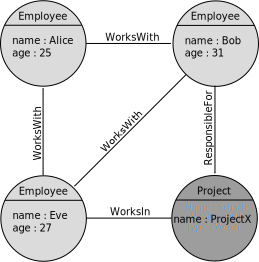
\includegraphics[scale=1]{orientdb_example.pdf}
	\caption[OrientDB: Beispielgraph]{Einfaches Beispiel eines Graphen mit den Knotenklassen \texttt{Employee} und \texttt{Project} sowie den Kantenklassen \texttt{WorksWith}, \texttt{WorksIn} und \texttt{ResponsibleFor}. Die \texttt{WorksWith}-Beziehung besitzt ein zus�tzliches Attribut, welches den Erstellzeitpunkt der Beziehung datiert.}
	\label{fig:orientdb_example}
\end{figure}

Abbildung \ref{fig:orientdb_example} zeigt einen schematisierten Graphen, welcher die Beziehungen zwischen Mitarbeitern und Projekten repr�sentiert, sowohl Knoten als auch Kanten sind Klassen zugeordnet. F�r deren Definition stellt OrientDB den \texttt{CREATE CLASS}-Operator zur Verf�gung. Nachfolgend wird eine Klasse \texttt{Employee} erzeugt, dieser wird ein Pflichtattribut \texttt{name} vom Typ \texttt{STRING} und ein optionales Attribut \texttt{age} vom Typ \texttt{INTEGER} zugewiesen. Mit der Angabe der Integrit�tsbedingung \texttt{MIN} erfolgt f�r Letzteres die Einschr�nkung zul�ssiger Werte.
Die Klasse selbst erbt von \texttt{V}, welche alle Knoten innerhalb des Graphen repr�sentiert. Die Definition der Klasse \texttt{Project} erfolgt analog.

\texttt{CREATE CLASS Employee EXTENDS V;}\newline
\texttt{CREATE PROPERTY Employee.name STRING;}\newline
\texttt{CREATE PROPERTY Employee.age INTEGER;}\newline
\texttt{ALTER PROPERTY Employee.name MANDATORY true;}\newline
\texttt{ALTER PROPERTY Employee.age MIN 18;}

Das Definieren von Kantentypen erfolgt ebenfalls mit dem gezeigten Operator, sie erben jedoch von \texttt{E}, der Klasse aller Kanten. Attribute werden wie bereits f�r Knoten gezeigt definiert. Nachfolgend ist stellvertretend der Befehl f�r das Anlegen des Kantentyps \texttt{WorksWith} dargestellt:

\texttt{CREATE CLASS WorksWith EXTENDS E;}

F�r die Manipulation der Datenbasis stehen in Standard-SQL die Befehle \texttt{INSERT}, \texttt{UPDATE} und \texttt{DELETE} zur Verf�gung. Diese werden auch in OrientDB angeboten, \texttt{INSERT} ist jedoch nur f�r die Verwendung mit Dokumenten vorgesehen, das Erzeugen von Knoten- und Kanteninstanzen erfolgt mit den Befehlen \texttt{CREATE VERTEX} bzw. \texttt{CREATE EDGE}. Die folgende Anweisung f�gt dem Graphen eine attributierte Knoteninstanz vom Typ \texttt{Employee} hinzu:

\texttt{CREATE VERTEX Employee SET name=\string"Alice\string", age=25;}

Das Erzeugen einer Kanteninstanz erfordert die Angabe der Identit�ten von Start- und Zielknoten, diese k�nnen entweder direkt angegeben, oder durch eine geschachtelte Selektion gelesen werden. Nachfolgend wird stellvertretend die Instanz der \texttt{WorksWith}-Beziehung zwischen den Mitarbeitern \texttt{Alice} und \texttt{Bob} eingef�gt, Kantenattribute k�nnen ohne Beachtung der Schemadefinition angef�gt werden:

\texttt{CREATE EDGE WorksWith}\newline
\texttt{FROM (SELECT FROM Employee WHERE name=\string"Alice\string")}\newline
\texttt{TO (SELECT FROM Employee WHERE name=\string"Bob\string")}\newline
\texttt{SET since=2011;}

\paragraph*{Mengenorientierte Operationen via OrientDB-SQL}

Die Informationsextraktion erfolgt entweder �ber den \texttt{SELECT}- oder den \texttt{TRAVERSE}-Operator. Analog zu Standard-SQL k�nnen diese beliebig geschachtelt werden. Die folgende Anfrage selektiert die Namen der Mitarbeiter zu denen \texttt{Alice} eine ausgehende Kante vom Typ \texttt{WorksWith} besitzt:

\texttt{SELECT name FROM}\newline
\texttt{(SELECT expand(out(\string"WorksWith\string")) FROM Employee WHERE name=\string"Alice\string");} 

Die Funktion \texttt{out} legt dabei die Richtung der Kante fest und kann wahlweise durch \texttt{in} oder \texttt{both} ersetzt werden. Das Ergebnis der drei Funktionen ist eine Menge von Knoten-Identit�ten, deren Instanzen durch \texttt{expand} aufgel�st werden und damit in �bergeordneten Anfragen verwendbar sind.\footnote{Sollen inzidente Kanten-Identit�ten selektiert werden, so ist dies mit den Funktionen \texttt{outE}, \texttt{inE} und \texttt{bothE} ebenfalls m�glich.} Das gezeigte Beispiel entspricht einer Verbundoperation in einem RDBMS. Der wesentliche Unterschied ist, dass die Beziehungsinformationen materialisiert an Knoten gespeichert sind und nicht zur Laufzeit berechnet werden m�ssen. Ersetzt man die Projektion der inneren \texttt{SELECT}-Anweisung durch: 

\texttt{expand(out(\string"WorksWith\string").out(\string"ResponsibleFor\string"))}

werden die Namen der Projekte ausgegeben, f�r welche die Kollegen von \texttt{Alice} verantwortlich sind. Handelt es sich bei beiden Beziehungen um $n:m$ Relationen, erfordert diese Anfrage in einer relationalen Datenbank vier Verbundoperationen. In OrientDB ist die Berechnung ausschlie�lich von der Anzahl der Beziehungen zwischen den einzelnen Knoteninstanzen abh�ngig.

Eine etwas komplexere Anfrage bezieht Kantenattribute mit ein und selektiert alle Kollegen von \texttt{Bob} mit denen er seit 2012 zusammenarbeitet und die �lter als 25 sind:

\texttt{SELECT since, in.name as name, in.age as age FROM}\newline
\texttt{(SELECT expand(outE(\string"WorksWith\string")) FROM Employee WHERE name=\string"Bob\string")}\newline
\texttt{WHERE since > 2011 AND in.age > 25;}

Die innere Anfrage selektiert mittels \texttt{outE} alle ausgehenden Kanten von \texttt{Bob}, welche anschlie�end durch das Pr�dikat \texttt{since > 2011} eingeschr�nkt werden. Die Funktion \texttt{in} verweist auf die Zielknoten der inzidenten Kanten, diese m�ssen den Attributschl�ssel \texttt{age} mit einem zugeh�rigen Wert gr��er als 25 aufweisen.

Aus den gezeigten Beispiel geht hervor, dass die Selektion durch die optionale Angabe einer \texttt{WHERE}-Klausel m�glich ist. OrientDB stellt vergleichende, boolesche und mathematische Operatoren f�r die Definition und Verkn�pfung von Pr�dikaten zur Verf�gung. Diese k�nnen in Verbindung mit einzelnen oder mehreren Attributwerten definiert werden. Ein Pr�dikat ber�cksichtigt ausschlie�lich Dokumente an denen das Attribut vorhanden ist, alle anderen sind nicht in der Ergebnismenge enthalten.\\
Die Projektion erlaubt die Auswahl einzelner Attribute aus der Ergebnismenge und erm�glicht die Berechnung von Aggregaten und das Ausf�hren von Funktionen.\\
Verschiedene Aggregatfunktionen, wie zum Beispiel \texttt{count}, \texttt{min}, \texttt{max} und \texttt{avg} stehen zur Verf�gung. Analog zu Neo4j erlaubt OrientDB die Verwendung zus�tzlicher skalarer, mathematischer, string-basierter und mengenorientierter Funktionen.\footnote{Eine vollst�ndige �bersicht �ber Operatoren und Funktionen findet sich unter \url{https://github.com/orientechnologies/orientdb/wiki/SQL-Where}.} Die Ergebnismenge kann gruppiert\footnote{In OrientDB 1.5.1 ist die Gruppierung nur f�r ein Attribut m�glich.}, sortiert sowie durch \texttt{SKIP} und \texttt{LIMIT} eingeschr�nkt werden.

% Traversierung
\paragraph*{Traversierung via OrientDB-SQL}

Das Pr�fen der Erreichbarkeit und das Berechnen von Pfaden ist in SQL ebenfalls m�glich. Der \texttt{TRAVERSE}-Operator f�hrt eine Traversierung ausgehend von einem konkreten Knoten oder einer Knotenmenge durch. Ein mehrfaches Besuchen von Knoten- und Kanteninstanzen wird durch das GDBMS verhindert, eine feingranulare Einstellm�glichkeit wie bei Neo4j oder die M�glichkeit zur manuellen Definition wie bei HyperGraphDB besteht nicht. Folgende Anfrage selektiert alle Knoten, die �ber eine \texttt{WorksWith}-Beziehung mit einem Startknoten verbunden sind und einen maximalen Abstand von drei zu diesem aufweisen:

\texttt{TRAVERSE out(\string"WorksWith\string") FROM \#11:0 WHILE \$depth<=3;}

Der Ausgangsknoten ist hierbei durch seine Identit�t \texttt{\#11:0} vorgegeben, alternativ k�nnen Klassen oder eingebettete Anfragen angegeben werden. Die Traversierung definiert einen abstrakten Weg, bei dem alle Kanten gerichtet und vom Typ \texttt{WorksWith} sind. Der Abstand zum Startknoten betr�gt h�chstens drei und wird sowohl zur Laufzeit als auch im Ergebnis an die Systemvariable \texttt{\$depth} gebunden. Das Ergebnis dieses Operators ist die Menge aller Knoten und Kanten, welche in den Instanzen des beschriebenen Weges enthalten sind. Diese lassen sich in �bergeordneten Anfragen weiter verarbeiten:

\texttt{SELECT name, min(\$depth) as dist FROM}\newline
\texttt{(TRAVERSE out(\string"WorksWith\string") FROM \#11:0 WHILE \$depth<=3 STRATEGY breadth\_first)}\newline
\texttt{GROUP BY name ORDER BY dist;}

Die gezeigte Anfrage listet alle Kollegen eines Mitarbeiters sortiert nach ihrem minimalen Abstand zueinander auf. Die \texttt{TRAVERSE}-Operation berechnet unter Verwendung der Breitensuche alle Pfadinstanzen.\footnote{Standardm��ig entspricht die Reihenfolge der zu traversierenden Knoten einem Tiefendurchlauf. Da Knoten jedoch systemseitig nicht mehrfach besucht werden k�nnen, weisen die gefundenen Pfadinstanzen nicht zwingend die minimale L�nge auf.} Da zwei Mitarbeiter �ber mehrere Pfade verbunden sein k�nnen, werden diese anschlie�end nach dem Namen des Kollegen gruppiert. Die Projektion schr�nkt die Ergebnismenge durch Aggregation der Pfadl�ngen mittels \texttt{min} ein.\\
Die Festlegung zu ber�cksichtigender Knotenbezeichner sowie von Knoten- und Kantenattributen erfolgt durch die Verwendung einer Selektion: Es sollen alle Projekte, mit denen ein Mitarbeiter direkt oder transitiv verbunden ist, zusammen mit dem Abstand zum Mitarbeiter ausgegeben werden:

\texttt{SELECT name, min(\$depth) FROM}\newline
\texttt{(TRAVERSE both() FROM \#11:0 WHILE \$depth<=4 STRATEGY breadth\_first)}\newline
\texttt{WHERE @Class=\string"Project\string" GROUP BY name;}

In dieser Anfrage werden durch die Verwendung von \texttt{both} ein- und ausgehende Kanten jeglichen Typs traversiert. Die Menge der Knoten wird durch das Pr�dikat \texttt{@Class=\string"Project\string"} auf Projekte eingeschr�nkt.

F�r das Berechnen k�rzester Pfade stellt OrientDB die Funktionen \texttt{shortestPath} f�r ungewichtete und \texttt{dijkstra} f�r gewichtete Graphen zur Verf�gung. Beide Funktionen unterst�tzen lediglich das Festlegen einer Kantenrichtung, Typ- oder Attributeinschr�nkungen sind weder f�r Knoten noch f�r Kanten m�glich.

%\paragraph*{Besonderheiten}
%
%- Hooks (Trigger)
%	- \url{https://github.com/orientechnologies/orientdb/wiki/Hook}
%- Functions 
%	- \url{https://github.com/orientechnologies/orientdb/wiki/Functions}
%	- Stored Procedures in JavaScript
%	- k�nnen via REST und auch embedded ausgef�hrt werden
%	- gegenseitiger Aufruf + Rekursion


\paragraph*{Transaktionen}

OrientDB unterst�tzt die Ausf�hrung von Zugriffen innerhalb von Transaktionen. Im Fall von SQL werden diese f�r �nderungen implizit erzeugt, der Commit erfolgt unmittelbar nach der Ausf�hrung. Alternativ k�nnen Transaktionen explizit begonnen, beendet und zur�ckgesetzt werden. Bei der Verwendung der Java API ist die Ausf�hrung von �nderungen nur in Verbindung mit dem expliziten Verwalten einer Transaktion m�glich. Analog zu HyperGraphDB l�sst sich die Transaktionsverwaltung beim Systemstart deaktivieren um zum Beispiel den Datenimport zu beschleunigen.

Im Gegensatz zu den bisher betrachteten Systemen wird das Schachteln von Transaktionen in OrientDB nicht unterst�tzt. Pro Thread im eingebetteten Betrieb bzw. pro Datenbankverbindung im Client-Server-Betrieb ist zu jedem Zeitpunkt nur eine Transaktion m�glich. Ist zum Beginn einer Transaktion bereits eine weitere aktiv, wird diese zur�ckgesetzt.

OrientDB bezeichnet sich selbst als ACID-konformes GDBMS: Zur Vermeidung von Mehrbenutzeranomalien wird das optimistische Synchronisationsverfahren MVCC eingesetzt, welches bereits im Zusammenhang mit HyperGraphDB beschrieben wurde. Die Ausf�hrung einer Transaktion erfolgt zun�chst ausschlie�lich innerhalb der Anwendung bzw. beim Client. Werden Objekte erzeugt, so erhalten sie eine tempor�re Identit�t, �nderungen an gelesenen Objekten erfolgen ebenfalls unabh�ngig vom GDBMS im Kontext der Anwendung.  Beim Commit werden alle Operationen an das Datenbanksystem �bertragen, dort werden sie chronologisch ausgef�hrt und die �nderungen in die Datenbasis eingebracht.\footnote{Die Speicherschicht ist w�hrend des Ausf�hrung des Commit exklusiv gesperrt, Dirty Reads werden somit vermieden. Dies kann im Quelltext unter \url{https://github.com/orientechnologies/orientdb/blob/1.5.1/core/src/main/java/com/orientechnologies/orient/core/storage/impl/local/OStorageLocalTxExecuter.java\#L83-L88} nachvollzogen werden.} Ein Konflikt liegt vor, wenn ein von der Transaktion ge�ndertes Objekt innerhalb der Datenbasis eine neue Version aufweist, in diesem Fall wird die Transaktion zur�ckgesetzt.\footnote{Dies kann im Quelltext unter \url{https://github.com/orientechnologies/orientdb/blob/1.5.1/core/src/main/java/com/orientechnologies/orient/core/storage/impl/local/OStorageLocal.java\#L1839-L1854} nachvollzogen werden.}\\
Im Gegensatz zu HyperGraphDB ber�cksichtigen Lesezugriffe nicht ausschlie�lich jene Objektversionen, die zu Beginn der Transaktion aktuell waren, stattdessen wird beim ersten Zugriff auf ein Objekt die neueste Version aus der Datenbasis geladen.\footnote{Dies entspricht dem Konzept der chronologieerhaltenden Serialisierbarkeit\cite{DBLP:books/sp/HarderR01}.} Alle nachfolgenden Lesezugriffe beziehen sich auf diese Objektversion. Daraus geht hervor, dass alle Mehrbenutzeranomalien vermieden werden, dies entspricht der Isolationsebene \texttt{SERIALIZABLE}.\footnote{Zu beachten ist, dass dies ausschlie�lich f�r die eingebettete Verwendung gilt. Im Client-Server-Betrieb werden Lesezugriffe immer vom Server beantwortet, folglich k�nnen die Anomalien Non-Repeatable Read und Phantom Problem auftreten. Dies entspricht der Isolationsebene \texttt{READ COMMITTED}. Die getroffenen Annahmen wurden durch den Entwickler best�tigt\cite{Orient_acid:2013}.}

Kommt es vor dem Commit einer Transaktion zum Ausfall des GDBMS oder des Clients, so sind die bis zu diesem Zeitpunkt erfolgten �nderungen nicht in der Datenbasis vorhanden, folglich ist in den genannten Situationen die atomare Ausf�hrung der Transaktion sichergestellt. Kommt es hingegen beim Ausf�hren des Commit zum Ausfall des GDBMS, k�nnen bereits Teile einer Transaktion in der Datenbasis vorhanden sein. Um diese �nderungen widerrufen zu k�nnen, wird vor dem Ausf�hren jeder �nderung ein zugeh�riger UNDO-Eintrag in ein Transaktions-Log geschrieben. Beim L�schen oder �ndern eines Datensatzes enth�lt der Eintrag eine Kopie des urspr�nglichen Datensatzes.\footnote{Dies entspricht dem Konzept des physischen Loggings\cite{DBLP:books/sp/HarderR01} und kann f�r das Aktualisieren im Quelltext unter \url{https://github.com/orientechnologies/orientdb/blob/1.5.1/core/src/main/java/com/orientechnologies/orient/core/storage/impl/local/OStorageLocalTxExecuter.java\#L115} nachvollzogen werden.} Das Ausschreiben der Log-Daten auf den Externspeicher erfolgt unmittelbar, beim Neustart des GDBMS kann somit ein konsistenter Zustand wiederhergestellt werden.\\
Bei der Betrachtung der Wiederholbarkeit erfolgreich beendeter Transaktionen muss zwischen den zwei verschiedenen, in OrientDB ausw�hlbaren, Speichermechanismen unterschieden werden: \texttt{OStorageLocal} und \texttt{OLocalPaginatedStorage}. Erstgenanntes nutzt Memory-Mapped-Files und �berl�sst es folglich dem Betriebssystem, wann ausgeschriebene �nderungen tats�chlich auf den Externspeicher geschrieben werden. Das zugeh�rige Transaktions-Log enth�lt jedoch keine REDO-Informationen erfolgreich beendeter Transaktionen. Folglich sind deren �nderungen verloren, wenn diese sich zum Zeitpunkt eines Systemausfalls noch nicht auf dem Externspeicher befinden.\footnote{Das GDBMS erm�glicht das Aktivieren einer FORCE-Strategie, bei der sowohl Log-Informationen als auch �nderungen an der Datenbasis unmittelbar auf den Externspeicher geschrieben werden. Dies kann jedoch mit Performance-Einbu�en verbunden sein\cite{DBLP:books/sp/HarderR01}.} Im Gegensatz dazu verwaltet \texttt{OLocalPaginatedStorage} den Zugriff auf den Externspeicher unabh�ngig vom Betriebssystem und f�hrt ein Transaktions-Log in dem sowohl UNDO- als auch REDO-Informationen gespeichert werden. Das Log selbst wird beim Commit auf den Externspeicher geschrieben, das Ausschreiben der eigentlichen �nderungen kann asynchron erfolgen, da die Log-Informationen ein Wiederherstellen im Fehlerfall erm�glichen.

\paragraph*{Indexverwaltung}

OrientDB unterst�tzt die Verwendung von Indexstrukturen f�r den effizienten Zugriff auf die gespeicherten Dokumente. Ein Index kann auf einem oder mehreren Attributen definiert werden und besitzt einen eindeutigen Bezeichner. Handelt es sich um ein schematisiertes Attribut, �bernimmt das GDBMS die Aktualisierung des Index, bei Attributen die nicht im Schema definiert sind, erfolgt die Verwaltung hingegen manuell. Es werden Befehle f�r das Einf�gen von Dokumenten, das Ausf�hren von Punkt- und Bereichsanfragen und das L�schen einzelner oder mehrerer Eintr�ge bereitgestellt. Dar�ber hinaus kann ein Index vollst�ndig entfernt werden.

Indizes k�nnen sowohl via Java API als auch in SQL definiert werden. Der nachfolgende Befehl erzeugt einen mehrdimensionalen Index auf den Attributen Name und Alter eines Mitarbeiters:

\texttt{CREATE INDEX idx1 ON Employee (name, age) UNIQUE;}

Der Indextyp \texttt{UNIQUE} erlaubt die Verwendung als Prim�rindex. Anzumerken ist, dass mehrdimensionale Indizes auch dann ber�cksichtigt werden, wenn nur eine der Dimensionen in einer \texttt{WHERE}-Klausel angegeben wird.

OrientDB beinhaltet zwei Index-Implementierungen: MVRB-Baum und Hash-Index. Der MVRB-Baum ist eine von Orient Technologies entwickelte Datenstruktur, welche die Eigenschaften des B$^+$-Baumes mit denen eines Rot-Schwarz-Baumes\cite{ottmann2002algorithmen} kombiniert. Die Struktur unterst�tzt Punkt- und Bereichsanfragen und kann als Indextyp \texttt{UNIQUE}, \texttt{NONUNIQUE}, \texttt{FULLTEXT} und \texttt{DICTIONARY} verwendet werden.\footnote{\texttt{DICTIONARY} ist identisch zu \texttt{UNIQUE}, existiert beim Einf�gen bereits ein entsprechender Eintrag wird dieser jedoch �berschrieben.} Indexoperationen sind logarithmisch von der Anzahl der Eintr�ge und der H�he des Baumes abh�ngig.\\
Eine zweite Implementierung basiert auf der Verwendung einer Hashtabelle, welche ausschlie�lich Punktanfragen unterst�tzt. Indexoperationen sind im besten Fall in konstanter Zeit m�glich, die nutzbaren Indextypen sind analog zum MVRB-Baum.
	
\subsection{Persistenz- und Cacheverwaltung}

Wie bereits im Zusammenhang mit Transaktionen genannt, unterst�tzt OrientDB zwei Speichermechanismen. Nachfolgend wird die Persistenzverwaltung anhand von \texttt{OStorageLocal} erl�utert, da diese Implementierung auch im sich anschlie�enden Benchmark verwendet werden wird. Laut Aussage der Entwickler soll \texttt{OLocalPaginatedStorage} in einer der folgenden Versionen die standardm��ige Implementierung sein\cite{Orient_acid:2013}, die offizielle Dokumentation enth�lt bisher jedoch keine detaillierten Informationen �ber den Speichermechanismus.

OrientDB ist ein natives GDBMS, da es Beziehungen zwischen Knoten physisch speichert und eine f�r Graphen optimierte Verarbeitung verspricht. Knoten und attributierte Kanten werden auf Dokumente abgebildet, die innerhalb der Speicherschicht als \textit{Record} bezeichnet werden. Ein Record ist genau einem \textit{Cluster} zugeordnet: Ein Cluster ist die physische Gruppierung von Records anhand einer definierten Eigenschaft. Dies kann der Typ oder ein beliebiges Attribut des Dokumentes sein. Bei der Verwendung des Typsystems wird f�r jede Klasse automatisch ein Cluster erzeugt.\footnote{Wird auf ein Schema verzichtet, werden alle Dokumente einem Cluster zugeordnet.} Dar�ber hinaus erlaubt das GDBMS aber auch das manuelle Zuweisen mehrerer Cluster zu einer Klasse:

\texttt{CREATE CLUSTER Projects2012;}\newline
\texttt{CREATE CLUSTER Projects2013;}\newline
\texttt{CREATE CLASS Project EXTENDS V CLUSTER Projects2012,Projects2013;}\newline
\texttt{CREATE VERTEX Project CLUSTER Projects2012 SET year=2012;}\newline
\texttt{CREATE VERTEX Project CLUSTER Projects2013 SET year=2013;}\newline
\texttt{SELECT FROM Project WHERE year=2013; // scans all clusters}\newline
\texttt{SELECT FROM cluster:Project2013; // scans one cluster}

In diesem Beispiel sind der Klasse \texttt{Project} zwei Cluster zugewiesen: \texttt{Projects2012} und \texttt{Projects2013}. Zwei Knoteninstanzen werden erzeugt und ihrem entsprechenden Cluster zugeordnet. Die gezeigten Leseanfragen besitzen eine identische Ergebnismenge, die zweite Anfrage kann jedoch effizienter ausgef�hrt werden, da lediglich ein Cluster ber�cksichtigt werden muss. Folglich l�sst sich durch Cluster eine semantische Gruppierung physisch abbilden. An dieser Stelle wird auch deutlich, warum OrientDB das Verwenden eines Schemas empfiehlt: Knoten und Kanten werden im Speichersystem gruppiert nach Typ verwaltet wodurch entsprechend eingeschr�nkte Anfragen effizienter beantwortet werden k�nnen.\\
Die Identit�t eines Records, die sog. \textit{RecordID} setzt sich aus der Identit�t des Clusters und der absoluten Position des Records innerhalb des Clusters zusammen: Ist zum Beispiel der Knoten \texttt{Alice} an Position 37 im Mitarbeiter-Cluster mit der Identit�t 13 gespeichert, dann ist die RecordID \texttt{\#13:37}.

Analog zu Neo4j wird die Datenbasis in OrientDB auf mehrere Dateien aufgeteilt. Hierbei erfolgt jedoch keine explizite Trennung in Topologie und Nutzdaten, stattdessen orientiert sich die Speicherung am Dokumentenmodell. Ein Cluster wird durch eine oder mehrere Dateien repr�sentiert. Jeder Eintrag innerhalb eines Clusters besitzt ein festes Format, was bedeutet, dass analog zu Neo4j die Berechnung der physischen Position effizient m�glich ist. Im Cluster werden keine Nutzdaten gespeichert, sie dienen lediglich der Gruppierung von Records, Cluster-Eintr�ge verweisen auf deren Nutzdaten. Diese befinden sich in der zweiten Komponente des Speichersystems, dem \textit{Data Segment}. 

\begin{figure}[h] 
	\centering
		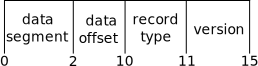
\includegraphics[scale=0.75]{orientdb_cluster_record.pdf}
	\caption[OrientDB: Datensatz eines Clusters]{Physische Repr�sentation eines Eintrags in einem Cluster in OrientDB. Der Datensatz hat eine feste L�nge von 15 Byte.\footnote{\url{https://github.com/orientechnologies/orientdb/blob/1.5.1/core/src/main/java/com/orientechnologies/orient/core/storage/impl/local/OClusterLocal.java?source=cc}}}
	\label{fig:orientdb_cluster_record}
\end{figure}

Abbildung \ref{fig:orientdb_cluster_record} zeigt den schematischen Aufbau eines Satzes in einem Cluster:
Die ersten zwei Byte verweisen auf das Data Segment, in welchem die Nutzdaten zu diesem Record hinterlegt sind, die nachfolgenden acht Byte legen die physische Position innerhalb des Data Segment fest. Die letzten f�nf Byte speichern Typ\footnote{Damit ist nicht der Datentyp gemeint. Ein Record kann entweder ein Dokument oder ein sog. Plain-Objekt sein. Letzteres ist f�r die Evaluation nicht relevant.} und Version des Dokumentes. Beim L�schen eines Datensatzes wird dessen Position in einer zus�tzlichen Datei vermerkt und steht f�r neue Dokumente zur Verf�gung.

Das Data Segment speichert die Nutzdaten eines Record und wird ebenfalls durch eine oder mehrere Dateien repr�sentiert. Da verf�gbare Informationen an Dokumenten individuell verschieden sein k�nnen, ist auch die L�nge eines Datensatzes variabel. Abbildung \ref{fig:orientdb_datasegment_record} zeigt dies schematisch.

\begin{figure}[h] 
	\centering
		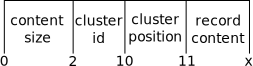
\includegraphics[scale=0.75]{orientdb_datasegment_record.pdf}
	\caption[OrientDB: Datensatz eines Datensegmentes]{Physische Repr�sentation eines Eintrags im Data Segment zur Speicherung der Nutzdaten. Der statische Teil des Datensatzes hat eine L�nge von 14 Byte, der dynamische Teil variiert je nach Umfang der hinterlegten Daten.}
	\label{fig:orientdb_datasegment_record}
\end{figure}

Ein Datensatz besteht aus einem Abschnitt fester L�nge und einem dynamischen Teil, welcher je nach Umfang der Nutzdaten verschieden gro� sein kann.\footnote{\url{https://github.com/orientechnologies/orientdb/blob/1.5.1/core/src/main/java/com/orientechnologies/orient/core/storage/impl/local/ODataLocal.java}} Die ersten vier Byte speichern die L�nge der Nutzdaten. Diese Information erm�glicht es, die Rohdaten aus dem Datensatz zu extrahieren um sie anschlie�end zu deserialisieren. Die nachfolgenden zehn Byte sind ebenfalls fest vergeben und enthalten Informationen �ber das zugeordnete Cluster. Der Rest des Datensatzes ist f�r die Speicherung der Rohdaten vorgesehen.

Das Auslesen der physischen Adressen im Cluster und im Datensegment ist in konstanter Zeit m�glich.
Daraus geht hervor, dass sich die Nachbarschaft eines Knotens $v$ analog zu Neo4j in $\mathcal{O}(\left|N_v\right|)$ berechnen l�sst. Dabei ist jedoch zu beachten, dass Beziehungsinformationen ebenfalls als Attribute in einem Dokument hinterlegt sind. Beim Lesen eines Records werden die kompletten Rohdaten geladen\footnote{Nachzuvollziehen unter \url{https://github.com/orientechnologies/orientdb/blob/1.5.1/core/src/main/java/com/orientechnologies/orient/core/storage/impl/local/ODataLocal.java?source=cc\#L248}}, das Deserialisieren der Nutzdaten erfolgt jedoch erst beim Zugriff auf das entsprechende Attribut.\footnote{Nachzuvollziehen unter \url{https://github.com/orientechnologies/orientdb/blob/1.5.1/core/src/main/java/com/orientechnologies/orient/core/record/impl/ODocumentHelper.java?source=c\#L224}.}  Folglich m�ssen beim Traversieren des Graphen die kompletten Rohdaten gelesen und die angefragten Kanten deserialisiert werden. Dar�ber hinaus stellen attributierte Kanten eine zus�tzliche Indirektion dar, da sie in einem dedizierten Dokument und damit auch in einem physisch unabh�ngigen Record gespeichert sind.

Beim L�schen eines Datensatzes im Data Segment werden Position und L�nge des Satzes in einer zus�tzlichen Datei hinterlegt und der somit definierte Bereich steht als freier Speicher zur Verf�gung. Aus der dynamischen L�nge des Satzes ergeben sich jedoch weitere Aufgaben: Beim Aktualisieren eines Dokumentes kann der zur Verf�gung stehende Speicher zu gering sein und das L�schen f�hrt zur Entstehung von freien Bereichen unterschiedlicher L�nge. Das GDBMS implementiert hierf�r eine Freispeicherverwaltung und eine automatische Defragmentierung. Eine detaillierte Betrachtung dieser Prozesse geht jedoch �ber den Rahmen dieser Arbeit hinaus und kann bei Bedarf anhand des Quelltextes nachvollzogen werden.

Eine dritte Komponente des Speichersystems ist der \textit{Storage}. Dieser nimmt Anfragen der Datenbankschicht entgegen und orchestriert den Zugriff auf Cluster und Data Segments.% Abbildung \ref{fig:orientdb_storage_sequence} fasst die Funktionsweise der Persistenzverwaltung am Beispiel des Lesens eines Dokumentes zusammen.

\paragraph*{Cacheverwaltung}

F�r den effizienten wahlfreien Zugriff auf deserialisierte Dokumente verwendet OrientDB mehrere Caches. Nachfolgend wird die Architektur im Kontext der eingebetteten Verwendung erl�utert.\\
Records werden aus dem Speichersystem geladen, deserialisiert und im Level-2-Cache abgelegt. Dabei handelt es sich um einen First-In-First-Out-Cache, welcher durch eine Hashtabelle mit verketteten Schl�sseln realisiert wird.\footnote{Es handelt sich um eine Erweiterung der Java-Datenstruktur \texttt{LinkedHashMap}. Dies kann unter \url{https://github.com/orientechnologies/orientdb/blob/1.5.1/core/src/main/java/com/orientechnologies/orient/core/cache/ODefaultCache.java?source=cc} nachvollzogen werden.} Der maximal nutzbare Hauptspeicher wird manuell festgelegt und bei �berschreiten dieser Grenze wird ein definierter Anteil der �ltesten Eintr�ge verdr�ngt. Alle Threads innerhalb der JVM k�nnen auf den Level-2-Cache zugreifen. Dar�ber hinaus ist jedem Thread ein dedizierter Level-1-Cache exklusiv zugeordnet. Dieser wird, vergleichbar mit HyperGraphDB, durch eine Hashtabelle und die Verwendung schwacher Referenzen realisiert.

Ein Lesezugriff pr�ft zun�chst, ob das angeforderte Dokument im Level-1-Cache vorhanden ist. Sollte dies nicht der Fall sein, erfolgt der Zugriff auf den Level-2-Cache. Befindet sich das Dokument dort, wird es in den Level-1-Cache bewegt. Ist das Dokument in keinem der Caches vorhanden, erfolgt der Zugriff auf das Speichersystem. Dieses besitzt einen eigenen Cache in dem die Ergebnisse von Lesezugriffen zwischengespeichert werden. Erst wenn der Record in diesem Cache nicht vorhanden ist, erfolgt der Zugriff auf den Hintergrundspeicher. Wie bereits erw�hnt, verwendet \texttt{OStorageLocal} Memory-Mapped-Files f�r die Abbildung der Daten auf den Externspeicher. Dies kann dazu f�hren, dass ein Lesezugriff ebenfalls aus dem Hauptspeicher beantwortet wird. 

Durch die client-seitige Ausf�hrung von Transaktionen, werden �nderungen an Dokumenten nicht unmittelbar im Cache reflektiert, die Aktualisierung erfolgt erst nach erfolgreicher Beendigung der Transaktion. Durch die Verwendung eines dedizierten Level-1-Caches pro Thread kann jedoch der Fall eintreten, dass sich ein Dokument mit verschiedenen Versionen in mehreren Level-1-Caches befindet. Um diesem Problem zu begegnen, kann entweder der Level-1-Cache vollst�ndig deaktiviert, oder das Zwischenspeichern eines Dokumentes explizit verboten werden. Bei der Verwendung mehrerer JVMs in Verbindung mit einer gemeinsamen physischen Speicherschicht, gilt gleiches auch f�r den Level-2-Cache.

\subsection{Verteilung und Skalierbarkeit}

OrientDB l�sst sich als verteiltes GDBMS einsetzen und unterst�tzt dabei die vollst�ndige Replikation der Datenbasis. Realisiert wird dies durch Hazelcast\footnote{\url{http://www.hazelcast.com/}}, einer quelloffenen, skalierbaren Verteilungsplattform f�r Java-Anwendungen. Im Gegensatz zu Neo4j verwendet OrientDB eine Muli-Master-Architektur\cite{rahm_masterslave}. Diese zeichnet sich dadurch aus, dass alle Rechner im Cluster gleichberechtigt sind: Lese- und insbesondere Schreibzugriffe k�nnen an allen Rechnern direkt ausgef�hrt werden. Nachfolgend wird die Architektur anhand der internen Ausf�hrung von �nderungs- und Lesetransaktionen kurz beschrieben.\footnote{Die offizielle Dokumentation enth�lt bez�glich der Datenverteilung nur wenig Informationen. Die vollst�ndige Evaluation des Quelltextes w�rde das Gewicht der Verteilung innerhalb der Evaluation nicht rechtfertigen.}

Erh�lt eine Instanz eine �nderungstransaktion, f�hrt sie diese zun�chst lokal durch. Anschlie�end erfolgt die Verteilung der �nderungen nach dem Push-Prinzip entweder synchron oder asynchron: Im synchronen Fall erh�lt der Client erst dann eine Best�tigung, wenn die �nderungen an allen Instanzen durchgef�hrt sind und folglich eine konsistente Sicht auf die Daten innerhalb des Clusters besteht. Im asynchronen Fall erfolgt die Best�tigung unmittelbar nachdem die Daten lokal geschrieben wurden, die Replikation der �nderungen erfolgt parallel bzw. verz�gert. Dies entspricht dem Konzept der Eventual Consistency, bei der das GDBMS f�r jede Instanz eine letztendlich konsistente Sicht auf die Daten garantiert.\\
Das Ausf�hren von Lesezugriffen ist ebenfalls an allen Rechnern im Cluster m�glich. Erfolgt die Replikation von �nderungen asynchron, k�nnen gelesene Daten eventuell veraltet sein, bei einer synchronen Replikation werden stets die aktuellen Daten gelesen.

Jede GDBMS-Instanz besitzt Informationen �ber alle weiteren Teilnehmer im Cluster, gleiches gilt auch f�r Client-Anwendungen. Beim Entfernen oder Hinzuf�gen einer Instanz wird die zugeh�rige Information an alle beteiligten Rechner propagiert. Daraus geht hervor, dass sich Clients beim Ausfall einer GDBMS-Instanz automatisch zu einer neuen Instanz verbinden und die Kommunikation fortsetzen k�nnen. Tritt eine neue Instanz dem Cluster bei, sendet diese zun�chst eine Anfrage zum Datenabgleich mit dem Verbund. Der Abgleich erfolgt auf Basis der Log-Informationen mit einer der verf�gbaren Instanzen. Diese sendet der neuen Instanz die entsprechende Differenzmenge an �nderungen zu.

% Skalierbarkeit
\paragraph*{Skalierbarkeit}

Die Multi-Master-Replikation erlaubt das horizontale Skalieren von Lese- und Schreibzugriffen. Zu beachten ist jedoch, dass dies f�r Schreibzugriffe nur im Fall einer asynchronen Replikation und auch da nur eingeschr�nkt gilt. �nderungsoperationen m�ssen an allen Instanzen durchgef�hrt werden, was je nach Anzahl der Rechner zu einer hohen Antwortzeit und somit bei hoher Schreiblast zu Performance-Problemen f�hren kann. Dar�ber hinaus muss die Korrektheit paralleler Schreibzugriffe generell und insbesondere auch beim Ausfall mehrerer Rechner sichergestellt sein. Bez�glich des maximalen Datenvolumens ist die Architektur ausschlie�lich vertikal skalierbar, da die Datenbasis an allen Instanzen komplett hinterlegt ist. Eine Partitionierung des Graphen wird aktuell entwickelt, ist jedoch weder dokumentiert noch in einer stabilen Version verf�gbar.\footnote{Der aktuelle Entwicklungsstand kann unter \url{https://github.com/orientechnologies/orientdb/tree/1.5.1/distributed/src/main/java/com/orientechnologies/orient/server/hazelcast} eingesehen werden.}
\section{Titan}

Das vierte System, welches im Rahmen der Evaluation betrachtet wird, ist Titan, ein quelloffenes, unter Apache 2.0 lizenziertes GDBMS. Es wird von der Firma Aurelius\footnote{\url{http://thinkaurelius.com/}} entwickelt und ist im Vergleich zu den bisher betrachteten Systemen ein sehr junges Projekt. Die erste Ver�ffentlichung erfolgte im September 2012, seit Mai 2013 ist die stabile Version 0.3.2 aktuell. Aurelius arbeitet eng mit dem TinkerPop-Projekt zusammen und implementiert die darin definierte Blueprints API. Titan selbst ist ausschlie�lich in Java umgesetzt, die Ausf�hrung ist somit auf kompatiblen Plattformen m�glich. Es handelt sich um ein GDBMS, in dem Modellierung und Verwendung der Daten nativ sind, Speicherung und Verarbeitung sind hingegen nicht-nativ: Der Graph wird analog zu HyperGraphDB auf ein Key-Value-Datenmodell abgebildet. Das verwendete Speichersystem ist austauschbar, Titan unterst�tzt aktuell die spaltenorientierten, verteilten Datenbanken Apache Cassandra\footnote{\url{http://cassandra.apache.org/}} und Apache HBase\footnote{\url{http://hbase.apache.org/}} sowie die bereits vorgestellte, zentrale Key-Value-Datenbank BerkeleyDB Java Edition. Die genannten Speichersysteme sind disk-orientiert, Titan bietet jedoch auch eine integrierte hauptspeicher-zentrierte Implementierung an. Die Verwendung des GDBMS erfolgt entweder eingebettet innerhalb von Java-Anwendungen oder im Client-Server-Betrieb.

Im Gegensatz zu den bisher betrachteten Systemen wird Titan prim�r f�r den Einsatz als verteiltes GDBMS entwickelt. Dabei nutzt es die Eigenschaften und Vorteile vorhandener Speichertechnologien f�r die horizontale Skalierung sowohl paralleler Zugriffe in als auch des Datenvolumens von umfangreichen Graphen. Aurelius definiert Graphen als umfangreich, wenn diese mehrere Milliarden Knoten und Kanten aufweisen.\footnote{Im Mai 2013 ver�ffentlichte Aurelius einen beeindruckenden Benchmark in dem die Performance paralleler Zugriffe auf einen Graph mit ca. 6 Milliarden Knoten und 121 Milliarden Kanten auf einem Titan-Cassandra-Cluster gemessen wurde. Die Ergebnisse k�nnen unter \cite{titan_bench:2013} eingesehen werden.} Entsprechend der vorgestellten Kategorisierung handelt es sich somit um eine Kombination aus Graphdatenbanksystem und Graph Processing System, welches Zugriffe mit lokalem Bezug auf umfangreichen Graphen erm�glicht. Eine weitere Besonderheit von Titan ist die Verwendung von Indizes an Knoten. Diese versprechen einen effizienteren Zugriff auf inzidente Kanten bei Knoten mit hohem Grad.

Die nachfolgenden Erl�uterungen beziehen sich auf Version 0.3.2 des GDBMS in Verbindung mit BerkeleyDB. Dies erm�glicht im nachfolgenden Benchmark den direkten Vergleich mit HyperGraphDB. Die verteilte Konfiguration der GDBMS wird im Benchmark nicht betrachtet, auf die Eigenschaften von Apache Cassandra und Apache HBase wird jedoch kurz in Abschnitt \ref{subsec:titan_verteilung} eingegangen. Die Informationen stammen vorrangig aus der offiziellen Dokumentation zu Titan\cite{titan_doku:2013} und Gremlin\cite{gremlin_doku:2013} sowie aus der offiziellen Mailing-Liste\cite{titan_mail:2013} des GDBMS.

\subsection{Datenmodell und Typsystem}

Titan implementiert das Property-Graph-Modell: Attribute k�nnen an Knoten und Kanten gespeichert werden, Kanten besitzen grunds�tzlich Richtung und Bezeichner. Attributschl�ssel sind vom Typ \texttt{String} w�hrend f�r Attributwerte s�mtliche primitiven Java-Datentypen sowie Arrays, Collections und Maps zul�ssig sind.\footnote{Titan verwendet die Java-Bibliothek Kryo f�r die (De-)Serialisierung von Objekten. Eine vollst�ndige Liste der unterst�tzten Datentypen kann unter \url{https://code.google.com/p/kryo/} eingesehen werden.} Abgesehen von Kantenbezeichnern ist die Definition eines Schemas an Knoten oder Kanten nicht m�glich, es lassen sich jedoch verschiedene Vorgaben festlegen, welche jedoch weniger auf die Modellierung einer Anwendungsdom�ne sondern mehr auf das effiziente Verwalten des Graphen ausgerichtet sind.

Das GDBMS verwendet spezielle Datentypen f�r Attributschl�ssel und Kantenbezeichner: \texttt{TitanKey} und \texttt{TitanLabel}. Diese lassen sich entweder manuell festlegen oder bei erstmaliger Verwendung eines Schl�ssels oder Bezeichners automatisch durch das System erzeugen. Das manuelle Vorgehen bietet mehrere Vorteile: Die M�glichkeit zur Definition von Integrit�tsbedingungen, eine verbesserte Speichereffizienz sowie eine erh�hte Performance. Typen definieren kein vollst�ndiges Knoten- oder Kantenschema; weist jedoch eine Instanz ein typisiertes Attribut oder Label auf, so m�ssen die geforderten Integrit�tsbedingungen eingehalten werden.

Typen besitzen einen systemweit eindeutigen Namen, dieser entspricht dem Attributschl�ssel bzw. dem Kantenbezeichner. Instanzen von \texttt{TitanKey} und \texttt{TitanLabel} k�nnen als \texttt{UNIQUE} deklariert werden: F�r Attributschl�ssel kann dies entweder auf einen einzelnen Knoten bzw. eine einzelne Kante oder auf den gesamten Graphen angewendet werden. Im ersten Fall darf dem entsprechend typisierten Attributschl�ssel an einer Knoten- oder Kanteninstanz h�chstens ein Wert zugeordnet sein, im zweiten Fall gilt die Einmaligkeit eines Schl�ssel-Wert-Paares systemweit. Standardm��ig kann ein Attributschl�ssel mehrfach an einem Knoten vorkommen.\\
F�r Kantenbezeichner kann hingegen festgelegt werden, ob entsprechend bezeichnete Instanzen in der Nachbarschaft eines Knotens einmalig sein m�ssen. Hierbei kann zwischen eingehenden und ausgehenden Kanten unterschieden werden. Beide Typen k�nnen gruppiert werden, dies erm�glicht ein effizienteres Abfragen von Attributen und Beziehungen eines Knotens.\footnote{Der Name eines Mitarbeiters ist ein Beispiel f�r ein einmaliges Attribut an einem Knoten w�hrend die Personalnummer innerhalb der gesamten Knotenmenge eindeutig sein muss. Ein Beispiel f�r eine einmalige Kante ist die Beziehung vom Angestelltem zum Vorgesetzten. Eine m�gliche Gruppierung von Kanten sind zum Beispiel die Beziehungen zwischen Mitarbeiter und Projekt gruppiert nach Abteilung.} 

Dar�ber hinaus definiert ein \texttt{TitanKey} den Datentyp des zugeordneten Attributwertes, was zum Einen dessen Wertebereich festlegt und zum Anderen die effizientere Speicherung erm�glicht. Des Weiteren k�nnen Attributschl�ssel indexiert und somit der direkte, effiziente Zugriff auf die zugeh�rigen Instanzen unter Angabe von Schl�ssel-Wert-Paaren realisiert werden. Im Unterschied dazu l�sst sich an einem \texttt{TitanLabel} ein Prim�rschl�ssel festlegen. Weist eine Kante das entsprechende Attribut auf, erlaubt dies das effizientere Auslesen inzidenter Kanten unter Angabe eines Wertes oder Wertebereiches.\footnote{Besitzt eine Beziehung vom Mitarbeiter zum Projekt einen Zeitstempel, welcher den Beitritt des Mitarbeiters datiert, und ist dieser Zeitstempel ein Prim�rschl�ssel, dann lassen sich Anfragen wie zum Beispiel \textit{In welchen Projekten hat Mitarbeiter x im Mai 2013 mitgearbeitet?} effizienter beantworten.} Dies ist ein Alleinstellungsmerkmal von Titan und verspricht eine h�here Performance beim Traversieren des Graphen. Aurelius bezeichnet dieses Konzept als \textit{vertex-centric indices}. Neben dem Prim�rschl�ssel kann ein Kantenbezeichner eine Signatur besitzen, die angibt, welche Attribute dies zugeh�rigen Kanteninstanzen besitzen bzw. voraussichtlich besitzen. Dies verspricht ein effizienteres Speichern und Laden von Kanteninstanzen. Kanten sind standardm��ig gerichtet und k�nnen in beiden Richtungen traversiert werden. Titan bietet hierf�r jedoch eine Einschr�nkung: Kanten k�nnen uni-direktional sein und nur vom Start- zum Zielknoten traversiert werden. Hierdurch kann Speicherplatz am Zielknoten gespart werden, zu beachten ist jedoch, dass ein L�schen des Zielknotens nicht das L�schen der Kante erfordert und das Einhalten der referentiellen Integrit�t somit in der Verantwortung der Anwendung liegt.

% Identit�t
Die Identit�t von Knoten- und Kanteninstanzen wird analog zu Neo4j durch eine 64-Bit-Ganzzahl festgelegt.\footnote{Nachzuvollziehen unter \url{https://github.com/thinkaurelius/titan/blob/0.3.2/titan-core/src/main/java/com/thinkaurelius/titan/core/TitanElement.java\#L52}.} Diese wird vom GDBMS vergeben und kann nach dem L�schen von Instanzen wiederverwendet werden. Unter Angabe einer Identit�t l�sst sich auf die Instanzen zugreifen, sie entspricht somit der Definition eines Prim�rschl�ssels.

% Anzahl der Datenbanken (wie Partitionierung)
Titan verwaltet genau eine Graphdatenbank, der alle Knoten und Kanten zugeordnet sind. Eine anwendungsseitige Partitionierung der Knoten- oder Kantenmenge ist ausschlie�lich durch die Verwendung dedizierter Attribute m�glich.

% Flexiblit�t
Aus den Ausf�hrungen geht hervor, dass Titan sehr flexibel bez�glich der expliziten Definition, �nderung und Verwendung eines Schemas ist. Analog zu Neo4j ist die Definition im Gegensatz zur Ber�cksichtigung von Kantenbezeichnern obligatorisch. �berl�sst man dem GDBMS das Erzeugen der Typen f�r Attributschl�ssel und Kantenbezeichner, so entspricht das Datenmodell exakt der Definition des PGM. Attribute lassen sich zur Laufzeit hinzuf�gen, �ndern und entfernen, Kantenbezeichner k�nnen hinzugef�gt, jedoch nicht ge�ndert oder gel�scht werden. Analog zu den bisher betrachteten GDBMS empfiehlt jedoch auch Aurelius die manuelle Typ-Definition um von den genannten Vorteilen zu profitieren.



\subsection{Zugriffsmechanismen, Transaktionen und Indexverwaltung}

% Varianten nennen (eingebettet, remote)
% Blueprints-Stack kurz erkl�ren
	- Integration in Neo4j, OrientDB, Dex, InfiniteGraph

% CRUD-Operationen analog zu OrientDB (+Typdefinition)
	% Unterschiede zu OrientDB aufzeigen (z.B. Typen statt Strings)
	% beliebig durch API
	% angebotene Algorithmen (entsprechend OrientDB im Furnace Paket)
	% imperativ
% Gremlin als wesentlicher Inhalt
	- Gremlin = DSL auf Basis von Groovy\footnote{\url{http://groovy.codehaus.org/}}, einer dynamischen Programmiersprache f�r die Java-Plattform
	- Titan erweitert Gremlin mit Hilfsmethoden
	% Paradigma (imperativ)
	% standardisiert (quasi-standard)
		% von allen GDBMS nutzbar, welche die Blueprints API implementieren
	% Definition
	% Manipulation (Einf�gen Knoten / Kante)
	% Traversierung
	% Mustersuche
	- https://github.com/tinkerpop/gremlin/wiki/SPARQL-vs.-Gremlin --> Testen
	% DSL
	- Groovy erm�glicht DSL\footnote{\url{http://thinkaurelius.com/2013/07/25/developing-a-domain-specific-language-in-gremlin/}}
	
\paragraph*{Transaktionen}

% obligatorisch
% Erzeugen (implizit, explizit)
% Schachtelung
% BerkeleyDB siehe OrientDB
	% Dauerhaftigkeit ist standardm��ig aktiviert (Quelltext)
	% REPEATABLE READ (keine Mehrbenutzeranomalien)
	% Behandlung von Deadlocks
% Transaktionen innerhalb von Titan?
- nur f�r inkonsistente Speichersysteme
	- MVCC
- Locks auf Unique Typen

Since edges and properties of unique labels and keys must be unique per vertex, inconsistencies could arise when two TitanGraph instances try to update the same unique edge or property concurrently, since one may overwrite the change of the other. To avoid such inconsistencies, Titan will acquire locks on unique edges and properties by default. Acquiring locks, however, can be very expensive depending on the storage backend. In cases where concurrent modifications can be excluded or blind overwrites are acceptable, a unique TitanType can be configured to not acquire locks by passing in UniquenessConsistency.NO\_LOCK as a second argument to TypeMaker.unique(). This configuration option should be used with care and only if the extra performance gain is needed.
	

% Anmerkung zu Cassandra und HBase

\paragraph*{Indexverwaltung}

% Primary Key
% Property-Index
- interne Indexstrukturen auf Attributen
\texttt{g.createKeyIndex("name", Vertex.class)}
	- Graph.query()
	- Besonderheiten: Geosuche, Volltextsuche

- externe Indeximplementierungen
	- ElasticSearch
	- Lucene

	% Aktualisierung (autmatische, manuelle Indizes)
	% Beispiel
% Vertex-centric Index!
- Vertex-Centric Indices
	- Supernode-Problem (Hubs, gro�e Nachbarschaft, sehr gro�er Knotengrad)
	- B-Baum zur Indizierung inzidenter Knoten erm�glicht schnellen Lookup bei Einschr�nkung auf Richtung, Kantenbezeichner und -attribute
		- disk-zentriertes Sortieren und Indexierung ->mehrdimensionaler Index
			- Kantenbezeichner -> Attribut
		- Vertex.query()
	- \texttt{final TitanKey time = graph.makeType().name(\string"time\string").dataType(Integer.class).makePropertyKey();}
	- \texttt{graph.makeType().name(\string"battled\string").primaryKey(time).makeEdgeLabel();}
	- $\mathcal{O}(\log(\left|N_v\right|))$
	

% Erweiterung?

\subsection{Persistenz- und Cacheverwaltung}

% https://groups.google.com/forum/?hl=de#!searchin/aureliusgraphs/storage$20single$20machine/aureliusgraphs/qO9Bi-y7uLs/EG5Ol-ulHjAJ

- Data Management
	- immutable atomic edges
	- OCC
	- feingranulares Locking auf Knoten- und Kantenebene
- Edge Compression

- Vertex-Centric Indizes
% BerkeleyDB: B-Baum, Transaktions-Log
% Abbildung des Graphen auf KV-Store (reicht!)
- Kantenkompression
	- Speicherung der ID-Differenz zwischen Ziel- und Startknoten
% Komplexit�t Nachbarschaft / Traversierung
- abh�ngig vom Speichersystem
	- BerkeleyDB logarithmisch

\paragraph*{Cacheverwaltung}

% BerkeleyDB
% eigene Caches

\subsection{Verteilung und Skalierbarkeit}
\label{subsec:titan_verteilung}

% BerkeleyDB ausschlie�lich zentral
% Replikation und Partitionierung via Cassandra / HBase
- Cassandra
	- Hochverf�gbarkeit (Replikation)
	- Peer-To-Peer Verteilung (Distributed Hashtable)
	- Caching
	- Eventual Consistency
- HBase
	- lineare Skalierbarkeit
	- Strong Consistency
	
% vielleicht kurz beschreiben (+Skalierbarkeit)

\section{Zusammenfassung und Zwischenfazit}

\paragraph*{Dokumentation}

Neo4j
	- sehr gute Dokumentation
	- Weg der L�nge $k$ f�hrt zu $\mathcal{O}(\left|N(v_1)\right| \times \left|N(v_2)\right| \times \cdots \times \left|N(v_k)\right|)$
	- Support auf Mailingliste

HyperGraphDB
	- gut Dokumentation
	- Support auf Mailingliste
	
OrientDB
	- Dokumentation sehr eingeschr�nkt, inkonsistent, viel Quelltextrecherche
	- Support auf Mailingliste
	
Titan
	- gute Doku f�r junges Projekt
	- Support auf Mailingliste
	
\paragraph*{Datenmodell}

% Tabelle

- Neo4j: PGM + Knotenlabel
	- keine Objekteinbettung
	- keine Schemadefinition an Knoten und Kanten
- HyperGraphDB: 
	- Atom-Modell sehr generisch
	- Schema durch Klassendefinition
- OrientDB: 
	- Dokumentmodell als Basis
	- PGM auf Dokumente abgebildet 
	- Schema durch Klassendefinition
- Titan: PGM + TitanKey + TitanLabel
	- keine Schemadefinition an Knoten und Kanten
	- Einschr�nkung der Attribute
	- Einschr�nkung der Kanten
	- Einschr�nkung Datentypen
	- verschachtelte Attributwerte (Maps)
	- Vertex-centric Indices
	- unidirektionale Kanten

\paragraph*{Zugriffsmechanismen}

CRUD-Operationen:
	- Neo4j: CRUD
		- in nativer API und Cypher m�glich
		- Algorithmen unterst�tzten Einschr�nkungen auf Graphen (im Gegensatz zu Blueprints)
	- HyperGraphDB: CRUD
	- OrientDB: CRUD
	- Titan: CRUD
Traversierung:
	- Neo4j:
		- algorithmische Traversierung mittels Traversal Framework -> Java
	- HyperGraphDB
		- algorithmische Traversierung mittels Traversal Framework -> Java
	- OrientDB
		- TRAVERSE-Operator oder Gremlin
	- Titan:
		- Gremlin, turing-m�chtig
Erreichbarkeit
	- Neo4j:
		- native API stellt Algorithmen zur Verf�gung
		- Cypher bietet shortestPath allShortestPath-Funktionen an
	- HyperGraphDB
		- durch Traversierung umsetzbar
		- Dijkstra-Implementierung
	- OrientDB
		- durch Traversierung umsetzbar
		- shortestPath und dijkstra in API
	- Titan
		- durch Traversierung umsetzbar
Mustersuche
	- Neo4j:
		- Cypher erm�glicht die Definition beliebiger Mustergraphen
	- HyperGraphDB
	 	- keine native Unterst�tzung
		- einfache Muster durch entsprechende Pr�dikatkombinationen
	- OrientDB
		- keine native Unterst�tzung
		- evtl. durch Schachtelung von SELECT und TRAVERSE
	- Titan
		- Musterdefinition via Gremlin und table-Funktion
		- weniger elegant als Cypher
Aggregation und Summierung
	- Neo4j:
		- Aggregation ja
		- Summierung nein
	- HyperGraphDB
		- Aggregation nein -> (hg.apply)
		- Summierung nein
	- OrientDB
		- Aggregation ja
		- Summierung nein
	- Titan
		- Aggregation ja
		- Summierung nein
Metriken
	- Neo4j: allShortestPaths -> grundlage f�r centrality ma�e
	- bis auf Kardinalit�t der Knoten- / Kantenmenge nichts zus�tzliches

Transaktionen
	- Neo4j: ACID, Locking, READ COMMITTED
	- HyperGraphDB: ACI(D), MVCC (GDBMS) + Locking (BerkeleyDB), SERIALIZABLE
	- OrientDB: ACID, MVCC, SERIALIZABLE
	- Titan: ACID, Locking (BerkeleyDB), SERIALIZABLE (BerkeleyDB)
	
\paragraph*{Speicherung und Caching}

- Neo4j: nativ
	- Trennung Topologie und Daten
	- Traversierung: O(1)
	- Fragmentierung der Stores
- HyperGraphDB: nicht-nativ
	- keine Trennung von Topologie und Daten
	- Speicherung in KV-Store 
	- Traversierung: O(logn)
- OrientDB: nativ
	- keine Trennung von Topologie und Daten 
	- Traversierung: O(N\_v)
	- Fragmentierung der Stores
	- attributierte Kanten sind zus�tzliche Indirektion\url{https://github.com/orientechnologies/orientdb/wiki/Performance-Tuning-Blueprints}
- Titan: nicht-nativ
	- keine Trennung von Topologie und Daten
	- Speicherung in KV-Store 
	- Traversierung O(logn)

- generell: Beschleunigung via Caches -> Hashtabellen  O(1) (wenn da)


OrientDB:
	- widerspr�chliche Dokumentation, wenig Beispiele
	- Bugs z.B. falsche Ergebnisse beim Traversieren, expand(shortestPath) und expand(dijkstra) haben 	kein Effekt

	- Ergebnisse zwischen Tiefen- und Breitensuche unterscheiden sich durch Verhindern des wiederholten Zugriffs

	- physische Repr�sentation: Deserialisieren der Attribute kann sich negativ auf Performance auswirken, attributierte Kanten ebenfalls

\paragraph*{Titan}

- Besonderheit: 
	- out-unique Einschr�nkung innerhalb der Instanz
	- in-unique entspricht Unique in Neo4j
	- verschachtelte Attributwerte
	- Vertex-centric Indices
	- unidirektionale Kanten




\chapter{Benchmark von Graphdatenbanksystemen}
\label{cha:benchmark}

In diesem Kapitel soll die Leistungsf�higkeit von Neo4j und Titan bei der Ausf�hrung graphenspezifischer Operationen bewertet werden. Dabei ist es von besonderem Interesse, ob sich die im vorhergehenden Kapitel aufgef�hrten funktionalen Unterschiede auf die Performance der GDBMS auswirken. Zus�tzlich soll beurteilt werden, inwieweit sich Cypher und Gremlin f�r die Formulierung analytischer Anfragen eignen. Zun�chst werden Testgraphen, Operationen und das Testsystem vorgestellt, anschlie�end wird auf die Konfiguration der einzelnen GDBMS sowie auf die Methodik bei der Durchf�hrung der Messungen eingegangen. Im zweiten, abschlie�enden Teil des Kapitels werden die Ergebnisse vorgestellt und bewertet.

\section{Testumgebung}

Bei der Analyse verwandter Arbeiten wurde festgestellt, dass aktuell - Stand Oktober 2013 - kein standardisierter Benchmark f�r GDBMS existiert. Die Herangehensweise fu�t auf den Empfehlungen von Dominguez-Sal et al.\cite{Dominguez-Sal2011}, da diese bereits in den verwandten Arbeiten von Ciglan et al.\cite{Ciglan:2012} und Gehrels\cite{Gehrels:2013} ber�cksichtigt wurden und somit als Quasi-Standard gewertet werden.

\subsection{Datengrundlage}

In Absprache mit dem Projektverantwortlichen wurde vereinbart, reale Datens�tze als Datengrundlage zu verwenden. F�r das in Abschnitt \ref{sec:anforderungen} beschriebene Forschungsvorhaben ist vorgesehen, Informationsnetzwerke aus unterschiedlichen Gesch�ftsinformationssystemen zu integrieren und den daraus resultierenden Graphen zu analysieren. Die Netzwerke in den Quellsystemen k�nnen dabei unterschiedliche topologische Eigenschaften aufweisen und die in ihnen gespeicherten Informationen verschiedenen Klassen zugeordnet sein. Ein ERP-System verwaltet zum Beispiel Rechnungen, w�hrend ein CRM-System vorrangig Kundenaktivit�ten speichert. Auf Grund der Wechselwirkungen zwischen den Entit�ten innerhalb der einzelnen Quellsysteme entstehen verschiedenartige Beziehungsstrukturen.Folglich ist der integrierte Graph bezogen auf Topologie und Nutzdaten heterogen.\\
Die Algorithmen zur Erzeugung von Zufallsgraphen, welche in den verwandten Arbeiten eingesetzt wurden, bilden ausschlie�lich homogene Netzwerke ab, in denen alle Klassen einer Dom�ne zugeordnet sind. In \cite{Vicknair:2010:CGD:1900008.1900067} sind es zum Beispiel Herkunftsinformationen innerhalb eines Entstehungsprozesses, in \cite{Holzschuher:2013:PGQ:2457317.2457351} Personen, Aktivit�ten, Organisationen und Nachrichten in einem sozialen Netzwerk, in \cite{Ciglan:2012}, \cite{Dominguez-Sal:2010:SGD:1927585.1927590} und \cite{Gehrels:2013} hingegen wird generell auf eine Klassifizierung der Informationen verzichtet. Das Erzeugen synthetischer, heterogener Graphen ist sehr aufw�ndig, da jeder Klasse und jeder Beziehungsart hinsichtlich ihrer Erzeugung eine eigene Logik zugeordnet werden muss.

Weil reale Daten aus Gesch�ftsinformationssystemen nicht frei zur Verf�gung stehen, werden stellvertretend f�r heterogene Netzwerke \texttt{amazon-meta}\cite{snap_amazon:2013} und \texttt{soc-Pokec}\cite{snap_pokec:2013} verwendet, beides Datens�tze des Stanford Network Analysis Project\footnote{\url{https://snap.stanford.edu/}}. Das Informationsnetzwerk \texttt{amazon-meta} beinhaltet Produktinformationen des Onlineh�ndlers Amazon\footnote{\url{http://www.amazon.com}}, wozu u.a. Produktbewertungen und Beziehungen zwischen Produkten z�hlen.\footnote{Es handelt sich dabei um �hnliche Produkte, die laut Amazon oft zusammen gekauft werden.} Pokec hingegen ist ein slowakisches soziales Online-Netzwerk, in dem Nutzer durch gerichtete Freundschaftsbeziehungen miteinander verbunden sind.\footnote{\url{http://pokec.azet.sk/}} Abbildung \ref{fig:testdata} zeigt das integrierte Schema beider Netzwerke als Property-Graph.

\begin{figure}[h] 
	\centering
		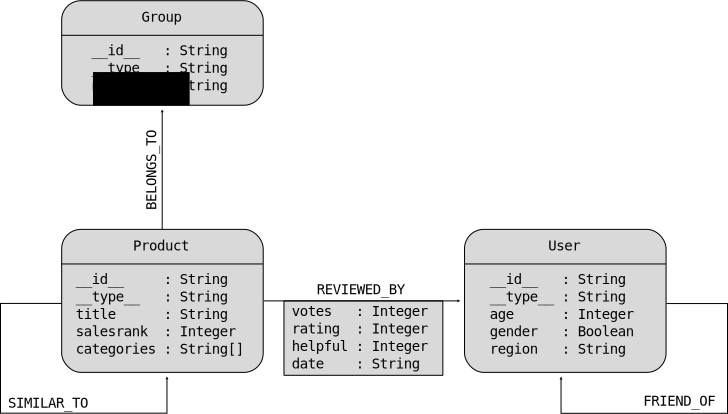
\includegraphics[scale=.75]{schema.pdf}
	\caption[Benchmark: Schema Testdaten]{Integriertes Schema aus Amazon- und Pokec-Daten.}
	\label{fig:testdata}
\end{figure}

Beide Datens�tze verf�gen �ber eine Klasse \texttt{User}. Deren Instanzen werden innerhalb von \texttt{amazon-meta} durch eine eindeutige Identit�t repr�sentiert und stehen nicht in Beziehung zueinander. In \texttt{soc-Pokec} hingegen weisen die Instanzen eine Vielzahl von Attributen auf und sind durch gerichtete \texttt{FRIEND\_OF}-Beziehungen miteinander verbunden. Die Anzahl der Nutzer stimmt in beiden Datens�tzen ann�hernd �berein, \texttt{amazon-meta} weist ca. 1.5 Mio., \texttt{soc-Pokec} etwa 1.6 Mio. Nutzer auf. Im Rahmen der Datenaufbereitung wurden zun�chst Pokec-Nutzer pseudozuf�llig auf Amazon-Nutzer abgebildet, anschlie�end wurde der durch die ausgew�hlten Knoten induzierte Teilgraph aus \texttt{soc-Pokec} extrahiert und mit \texttt{amazon-meta} zu einem integrierten Graph zusammengef�hrt.\\
Die Netzwerke enthalten neben den topologischen Informationen auch Nutzdaten, welche f�r Gruppen, Produkte und Bewertungen vollst�ndig aus den Rohdaten �bernommen wurden, f�r die Nutzer hingegen wurde eine Auswahl von Attributen unterschiedlichen Datentyps getroffen. Die Rohdaten beider Netzwerke wurden f�r die weitere Verwendung in das textbasierte Geoff-Format\footnote{\url{http://nigelsmall.com/geoff}} �berf�hrt, welches von Neo4j entwickelt wurde.

\renewcommand{\arraystretch}{1.25}
\begin{table}[h]
	\centering
	\begin{footnotesize}
   	\begin{tabular}{|l|rl|rl|rl|rl|rl|rl|rl|rl|rl|}
	\hline
   	 & \multicolumn{8}{c|}{\textbf{Knoten}} & \multicolumn{2}{c|}{\textbf{Attribute}} \\ \cline{2-11}
   	\textbf{Graph} & \multicolumn{2}{c|}{\texttt{Group}} & \multicolumn{2}{c|}{\texttt{Product}} & \multicolumn{2}{c|}{\texttt{User}} & \multicolumn{2}{c|}{$\Sigma$} & \multicolumn{2}{c|}{$\Sigma$} \\
   	\hline
   	   	\hline
   	\texttt{orig} & \multicolumn{2}{c|}{10} & \multicolumn{2}{c|}{542\,684} & \multicolumn{2}{c|}{1\,555\,124} & \multicolumn{2}{c|}{2\,097\,819} & \multicolumn{2}{c|}{20\,377\,902} \\
   	\hline
   	\hline
	\texttt{p\_100} & 1 & (1) & 126 & (1) & 347\,752 & (1) & 347\,879 & (1) & 1\,874\,907 & (1)\\
	\hline
	\texttt{p\_1K} & 4 & (4) & 1\,089 & (8.64) & 665\,116 & (1.91) & 666\,209 & (1.92) & 3\,710\,473 & (1.98) \\
	\hline
	\texttt{p\_10K} & 4 & (1) & 10\,047 & (9.23) & 976\,985 & (1.47) & 987\,036 & (1.47) & 7\,255\,153 & (1.96) \\
   	\hline
  	\end{tabular} 
	\end{footnotesize}
	\setlength{\belowcaptionskip}{0.25cm}	
	\caption[Benchmark: Anzahl Knoten und Attribute]{Anzahl Instanzen der verschiedenen Knotenklassen und Gesamtanzahl der Knoten- und Kantenattribute.}
		\label{tab:datasets_nodes}
\end{table}
\renewcommand{\arraystretch}{1}

\renewcommand{\arraystretch}{1.25}
\begin{table}[h]
	\centering
	\begin{footnotesize}
   	\begin{tabular}{|l|rl|rl|rl|rl|rl|}
	\hline
	& \multicolumn{10}{c|}{\textbf{Kanten}} \\ \cline{2-11}

   	\textbf{Graph} & \multicolumn{2}{c|}{\texttt{BELONGS\_TO}} & \multicolumn{2}{c|}{\texttt{SIMILAR\_TO}} & \multicolumn{2}{c|}{\texttt{REVIEWED\_BY}} & \multicolumn{2}{c|}{\texttt{FRIEND\_OF}} & \multicolumn{2}{c|}{$\Sigma$} \\
   	\hline
   	\hline
   	\texttt{orig} & \multicolumn{2}{c|}{542\,684} & \multicolumn{2}{c|}{1\,231\,400} & \multicolumn{2}{c|}{7\,593\,109} & \multicolumn{2}{c|}{27\,787\,537} & \multicolumn{2}{c|}{37\,154\,730} \\
	\hline
	\hline
	\texttt{p\_100} & 126 & (1) & 396 & (1) & 1\,909 & (1) & 704\,092 & (1) & 706\,523 & (1) \\
	\hline
	\texttt{p\_1K} & 1\,089 & (8.64) & 3\,365 & (8.5) & 29\,848 & (15.64) & 1\,830\,064 & (2.6) & 1\,864\,366 & (2.64) \\
	\hline
	\texttt{p\_10K} & 10\,048 & (9.23) & 27\,976 & (8.31) & 401\,917 & (13.47) & 3\,576\,276 & (1.95) & 4\,016\,216 & (2.15) \\
	\hline
  	\end{tabular} 
	\end{footnotesize}
	\setlength{\belowcaptionskip}{0.25cm}	
	\caption[Benchmark: Anzahl Kanten]{Anzahl Instanzen der verschiedenen Kantenbezeichner.}
	\label{tab:datasets_edges}
\end{table}
\renewcommand{\arraystretch}{1}

Ein wichtiges Kriterium bei der Durchf�hrung eines Benchmarks ist das Leistungsverhalten einer Anfrage bei steigendem Datenvolumen. Synthetische Datens�tze lassen sich erzeugen, reale Datens�tze hingegen besitzen eine festgelegte Gr��e. Mit dem Ziel, die Skalierbarkeit von Anfragen dennoch untersuchen zu k�nnen, wurden zusammenh�ngende Teilgraphen aus dem integrierten Datensatz extrahiert. Die Teilgraphen sind bez�glich der Knoten aus \texttt{amazon-meta} induziert, dies gilt nicht f�r den Teilgraph, welcher ausschlie�lich aus Nutzerknoten besteht. Der Algorithmus wird in Anhang \ref{anh:extraction} beschrieben.

Dominguez-Sal et al. empfehlen die Angabe eines einzelnen Skalierungsfaktors, von welchem die Anzahl der erzeugten Knoten und Kanten abh�ngig ist, dies l�sst sich jedoch bei der Verwendung realer Datens�tze nicht umsetzen. Durch die Wahr der Parameter des Extraktionsalgorithmus wurde daher versucht, m�glichst konstante Wachstumsfaktoren zu erreichen. Die Tabellen \ref{tab:datasets_nodes} und \ref{tab:datasets_edges} stellen den integrierten Graph (\texttt{orig}) und die extrahierten Teilgraphen bezogen auf die Anzahl der Knoten und Kanten gruppiert nach ihrer jeweiligen Klasse gegen�ber. Zus�tzlich wird der Wachstumsfaktor f�r jeden Wert in Relation auf dessen �quivalent im n�chstkleineren Graphen angeben. Ein Nachteil dieser Herangehensweise ist, dass sich die topologischen Eigenschaften der verschiedenen extrahierten Teilgraphen unterscheiden k�nnen, was bei der nachfolgenden Bewertung ber�cksichtigt wird.

\subsection{Operationen}

Stellvertretend f�r jene Anfragen, welche f�r die Analyse von Unternehmensdaten im Forschungsvorhaben relevant sind, wurden auf Grundlage des vorgestellten Schemas mehrere Anfragen definiert, die jeweils einzelne oder mehrere der in Abschnitt \ref{subsec:graph_operations} vorgestellten graphenspezifischen Operationen beinhalten. Es handelt sich um lokale Anfragen, die ausgehend von einem Knoten oder einer Knotenmenge einen Teil des Graphen analysieren. Dabei werden seine Topologie und auch Nutzdaten in die Operationen einbezogen. Es wurde bewusst auf rein topologische und globale Anfragen verzichtet, da sie f�r das Forschungsvorhaben nicht relevant sind, Beispiele hierf�r sind das Berechnen der k-Nachbarschaft ohne Ber�cksichtigung von Kantenbezeichnern oder das Auslesen aller Kanten. Gleiches gilt f�r Schreibzugriffe, hier ist lediglich die Performance der Bulk-Load-Mechanismen von Interesse. 

\renewcommand{\arraystretch}{1.25}
\begin{table}[h]
	\centering
	\begin{footnotesize}
   	\begin{tabular}{|m{2.3cm}|>{\arraybackslash}m{13.45cm}|}
	\hline
   	\multicolumn{1}{|c|}{\textbf{Name}} & \multicolumn{1}{c|}{\textbf{Beschreibung (Kategorisierung der Operationen)}} \\
	\hline
	\hline
	\textbf{\texttt{import}} & Importieren der Testgraphen in das jeweilige GDBMS unter Verwendung von Bulk-Load-Mechanismen. (Schreibperformance beim Bulk-Load)\\
	\hline
	\textbf{\texttt{random\_read}} & Zuf�llige Auswahl einzelner Produkte und Nutzer sowie vollst�ndiges Auslesen ihrer Attribute. (Leseperformance beim Attributzugriff) \\
	\hline
	\textbf{\texttt{sim\_products}} & Zuf�llige Auswahl eines Produktes und anschlie�endes Traversieren  �hnlicher Produkte bis Abstand $\leq$ 2, die Kantenrichtung ist nicht relevant. Die Produkttitel sollen ausgegeben werden, jeder Titel soll einmalig in der Ergebnismenge sein. (Lokale Traversierung, Einschr�nkung) \\
	\hline
	\textbf{\texttt{foaf\_reviews}} & Zuf�llige Auswahl eines Nutzers und anschlie�ende Selektion der Produkte, f�r die Freunde oder deren Freunde ein Review geschrieben haben. Das Ergebnis soll nach Produkttitel gruppiert und nach durchschnittlicher Bewertung sortiert werden. (Lokale Traversierung, Einschr�nkung, Gruppierung, Aggregation)\\
	\hline
	\textbf{\texttt{path\_all}} & Zuf�llige Auswahl eines Nutzers und eines Produktes und anschlie�endes Berechnen aller Pfade der L�nge $\leq 4$ zwischen beiden Knoten. Dabei sollen nur die Kantenbezeichner \texttt{FRIEND\_OF}, \texttt{REVIEWED\_BY} und \texttt{SIMILAR\_TO} ber�cksichtigt werden, die Kantenrichtung ist nicht relevant. Im Ergebnis sollen die Pfade gruppiert nach L�nge und der jeweiligen Anzahl ausgegeben werden. (Erreichbarkeit, Einschr�nkung, Gruppierung, Aggregation) \\
	\hline
	\textbf{\texttt{path\_shortest}} & Zuf�llige Auswahl zweier Nutzer und anschlie�ende Berechnung des k�rzesten Pfades unter Ber�cksichtigung der Kantenbezeichner \texttt{FRIEND\_OF}, \texttt{REVIEWED\_BY} und \texttt{SIMILAR\_TO}. Die maximale Pfadl�nge betr�gt 4, Kantenrichtungen werden nicht ber�cksichtigt. Das Ergebnis soll das Attribut \texttt{\_\_id\_\_} der Knoten innerhalb des Pfades beinhalten. (Erreichbarkeit, Einschr�nkung) \\
	\hline
	\textbf{\texttt{top\_regions}} & Auswahl aller Produkte, welche der Gruppe \texttt{'Books'} angeh�ren und das Pr�dikat \texttt{salesrank} $\leq$ 500\,000 erf�llen. Das Ergebnis soll nach dem Attribut \texttt{region} jener Nutzer gruppiert werden, welche die Produkte mit einem \texttt{rating} $\geq$ 3 bewertet haben und dies f�r $\geq$ 5 Nutzer hilfreich war. Dar�ber hinaus soll das Ergebnis nach der Anzahl der Produkte pro Region sortiert und die oberen 10 Regionen ausgegeben werden. (Lokale Traversierung, Aggregation, Gruppierung, Selektion) \\
	\hline
	\textbf{\texttt{sim\_pattern}} & Zuf�llige Auswahl eines Nutzers und anschlie�endes Bestimmen seiner Freunde, die f�r mindestens ein �bereinstimmendes Produkt Reviews geschrieben haben. Das Ergebnis soll den Nutzer selbst, die Freunde des Nutzers und die �bereinstimmende Produktmenge beinhalten. (Lokale exakte Mustersuche) \\
	\hline
  	\end{tabular} 
	\end{footnotesize}
	\setlength{\belowcaptionskip}{0.25cm}	
	\caption[Benchmark: Beschreibung der einzelnen Anfragen]{Namen und Beschreibungen der durchzuf�hrenden Anfragen.}
	\label{tab:benchmark_queries}
\end{table}
\renewcommand{\arraystretch}{1}

In Tabelle \ref{tab:benchmark_queries} werden die Anfragen beschrieben und entsprechend der verwendeten Operationen kategorisiert. Alle Anfragen wurden mittels Cypher und Gremlin realisiert und sind in Anhang \ref{anh:queries} aufgef�hrt. Eine Implementierung unter Verwendung der vorhandenen Java APIs wurde nicht durchgef�hrt, da in dieser Arbeit die Verwendung aktueller graphenspezifischer Anfragesprachen f�r die Formulierung komplexerer, analytischer Anfragen vordergr�ndig ist. Bereits in \cite{Ciglan:2012}, \cite{Gehrels:2013} und \cite{Holzschuher:2013:PGQ:2457317.2457351} wurde gezeigt, dass sich der Verzicht auf eine zus�tzliche Anfrageverarbeitung positiv auf das Leistungsverhalten auswirkt. Eine Eignung der APIs f�r die Implementierung beliebiger analytischer Algorithmen und Operationen wurde den Systemen bereits im vorhergehenden Kapitel attestiert.

\subsection{Systemkonfiguration}

Die verwendete Testumgebung setzt sich wie folgt zusammen:

\begin{itemize}
	\setlength{\parskip}{1pt}
	\item Intel i7-2620M (2x3.4 Ghz)
	\item 8 GB DDR-3 RAM (1333 Mhz)
	\item Crucial M4 SSD (128 GB)
	\item Xubuntu 13.10 64-Bit (Kernel 3.11.0-12-generic, ext4)
	\item Java(TM) SE Runtime Environment (build 1.7.0\_45-b18)
\end{itemize}

\paragraph*{Neo4j}

Das GDBMS wird in einer zentralen, eingebetteten Konfiguration verwendet, Anfragen werden sowohl in Cypher als auch in Gremlin ausgef�hrt. F�r Cypher-Anfragen wird die im vorhergehenden Kapitel betrachtete Version 2.0.0-M04 eingesetzt. Die Ber�cksichtigung von Gremlin erm�glicht eine bessere Vergleichbarkeit mit Titan, macht es jedoch erforderlich, f�r die Durchf�hrung auf Version 1.9.4 des GDBMS zur�ckzugreifen, da Blueprints 2.4.0 und somit auch Gremlin bisher nicht kompatibel zu den Neuerungen in Neo4j 2.0 sind.  Die Ausf�hrung von Cypher erfolgt unter Verwendung der \texttt{ExecutionEngine}\footnote{\url{http://docs.neo4j.org/chunked/2.0.0-M04/tutorials-cypher-java.html}}, f�r Gremlin wird die in der Dokumentation beschriebene \texttt{GremlinGroovyScriptEngine} \footnote{\url{https://github.com/tinkerpop/gremlin/wiki/Using-Gremlin-through-Java\#using-jsr-223-gremlingroovyscriptengine}} genutzt.

F�r den Bulk-Load der Testgraphen wird im \texttt{import}-Benchmark der von Neo4j zur Verf�gung gestellte \texttt{BatchInserter} entsprechend der Dokumentation\footnote{\url{http://docs.neo4j.org/chunked/2.0.0-M04/batchinsert.html}} eingesetzt. W�hrend des Import erfolgt das Aktualisieren eines zus�tzlichen Lucene-Index auf dem Knotenattribut \texttt{\_\_id\_\_}. Bei der Verwendung von Neo4j 2.0.0-M04 werden dar�ber hinaus Knotenbezeichner entsprechend der Knotenklasse gesetzt, diese k�nnen folglich nur in Cypher-Anfragen ber�cksichtigt werden.

Die Kernel-Einstellungen\footnote{\url{http://docs.neo4j.org/chunked/2.0.0-M04/kernel-configuration.html}} des GDBMS werden unver�ndert �bernommen. Die Gr��e des Heap-Speichers der JVM wird entsprechend den Empfehlungen\footnote{\url{http://docs.neo4j.org/chunked/2.0.0-M04/configuration-jvm.html}} auf 4 GB festgelegt, eine �nderung des Stack-Speichers erfolgt nicht. Dar�ber hinaus wird der Concurrent Mark and Sweep Compactor Garbage Collector\footnote{\url{http://www.oracle.com/technetwork/java/javase/tech/vmoptions-jsp-140102.html\#BehavioralOptions}} verwendet.\\
Die Einstellungen des Object-Cache bleiben unver�ndert, es wird demnach die in Abschnitt \ref{subsec:neo4j_persistency} beschriebene Standard-Implementierung genutzt. Der Filesystem-Cache wurde entsprechend der Gr��e der Stores angepasst. Um deren Speicherbedarf zu ermitteln, wurde der gr��te Testgraph (\texttt{p\_10K}) importiert und die Gr��e der Stores im Dateisystem bestimmt. F�r den Knoten-Store sind dies 20 MB, f�r den Kanten-Store 150 MB.\footnote{Dieser Wert l�sst sich ebenfalls aus der Datensatzgr��e von 14 bzw. 33 Byte und der Anzahl Knoten bzw. Kanten in Tabelle \ref{tab:datasets_nodes} bzw. \ref{tab:datasets_edges} berechnen.} Interessant ist, dass trotz der Verwendung von String- und Array-Properties der Property-Store f�r primitive Datentypen den gr��ten Speicherbedarf aufweist.\footnote{F�r primitive Datentypen werden 150 MB, f�r Strings 50 MB und f�r Arrays 10 MB beansprucht.} Neo4j verwendet f�r Strings und Arrays zus�tzliche Kompressionsmethoden\footnote{\url{http://docs.neo4j.org/chunked/2.0.0-M04/short-strings.html} und \url{http://docs.neo4j.org/chunked/2.0.0-M04/short-arrays.html}} und f�gt, wenn m�glich, die entsprechenden Werte in den Property-Store f�r primitive Datentypen ein und vermeidet damit eine zus�tzliche Indirektion beim Lese- und Schreibzugriff. Die Anpassung des Filesystem-Cache erm�glicht es dem GDBMS die komplette Datenbasis im Hauptspeicher vorhalten zu k�nnen.

\paragraph*{Titan}

Das GDBMS wird ebenfalls in einer zentralen, eingebetteten Konfiguration verwendet. Anfragen werden ausschlie�lich in Gremlin ausgef�hrt, dies erfolgt wie bei Neo4j unter Verwendung der \texttt{GremlinGroovyScriptEngine}. Das verwendete Speichersystem ist BerkeleyDB Java Edition, die Konfiguration erfolgt ausschlie�lich mit den von Titan zur Verf�gung gestellten Parametern.

F�r den Import der Testgraphen wird der im TinkerPop-Projekt verf�gbare \texttt{BatchGraph} verwendet, eine Wrapper-Klasse, die Bulk-Load-Funktionalit�t f�r blueprints-kompatible GDBMS zur Verf�gung stellt.\footnote{\url{https://github.com/tinkerpop/blueprints/wiki/Batch-Implementation}} Die Verwendung von \texttt{BatchGraph} wird von Aurelius f�r Graphen mit bis zu 100 Mio. Kanten empfohlen. Dar�ber hinaus wurde der Konfigurationsparameter \texttt{storage.batch-loading} auf \texttt{true} gesetzt, was die internen Konsistenzmechanismen von Titan deaktiviert und den Import beschleunigen soll.\\
Vor dem Datenimport werden Instanzen von \texttt{TitanKey} bzw. \texttt{TitanLabel} erzeugt. F�r Instanzen von \texttt{TitanKey} werden Attributschl�ssel, Datentyp des Attributwertes und Eindeutigkeit an der Instanz festgelegt, dem Knotenattribut \texttt{\_\_id\_\_} wird wie bei Neo4j ein Index zugeordnet. Die Instanzen von \texttt{TitanLabel} werden entsprechend den vier Beziehungsarten bezeichnet, \texttt{BELONGS\_TO}-Kanten werden dar�ber hinaus als $n:1$-Beziehung zwischen Produkt und Gruppe deklariert. Die Durchf�hrung erfolgt sowohl mit manueller als auch mit systemseitiger Typdefinition, damit soll untersucht werden, inwieweit sich die Festlegung der Datentypen auf die Leistungsf�higkeit des GDBMS auswirkt.

Entsprechend der Empfehlung von Aurelius werden BerkeleyDB 80\% des zur Verf�gung stehenden Heap-Speichers zur Verf�gung gestellt.\footnote{\url{https://github.com/thinkaurelius/titan/wiki/Using-BerkeleyDB}} Dieser wird wie bei Neo4j auf insgesamt 4 GB festgelegt. Oracle empfiehlt f�r BerkeleyDB ebenfalls die Verwendung des Concurrent Mark and Sweep Compactor Garbage Collector, welcher folglich bei der Durchf�hrung aktiviert ist.\footnote{\url{http://www.oracle.com/technetwork/database/berkeleydb/je-faq-096044.html\#WhatJVMparametersshouldIconsiderwhentuninganapplicationwithalargecachesize}}

\subsection{Methodik}

% Verweis auf Framework
F�r die Durchf�hrung der Messungen wurde ein Java-Framework\footnote{\url{https://github.com/s1ck/master_thesis/tree/master/benchmark}} entwickelt, mit dem sich individuell konfigurierbare Benchmarks nach einem definierten Protokoll ausf�hren lassen. Jede der zu messenden Anfragen kann einzeln aktiviert und konfiguriert werden. Dabei l�sst sich die Ausf�hrungsreihenfolge beliebig variieren, bei der Durchf�hrung wird die Reihenfolge entsprechend Tabelle \ref{tab:benchmark_queries} beibehalten.

% Import
Die Testgraphen liegen im Geoff-Format vor und werden unter Verwendung eines Iterators eingelesen. Dieser Ansatz erm�glicht es, auch umfangreiche Datens�tze ohne zus�tzliche Inanspruchnahme des Hauptspeichers zu verarbeiten und gleichzeitig die unmittelbare Schreibperformance des GDBMS in Abh�ngigkeit vom Externspeicher zu messen.

% Warmup Caches
F�r die Simulation eines realistischen Antwortzeitverhaltens empfehlen Dominguez-Sal et al. ein sog. \textit{warmup} der Caches. Eine Zielstellung des Forschungsvorhabens ist die Verwendung des GDBMS im Rahmen einer Analyseplattform. Dabei wird angenommen, dass diese nicht nur bei Bedarf gestartet wird, sondern permanent in Betrieb ist. Folglich ist davon auszugehen, dass sich entweder der gesamte Graph oder Teilgraphen zum Zeitpunkt der Anfrage in den Caches befinden und somit eine effizientere Ausf�hrung m�glich ist.\\ % Dar�ber hinaus verdeutlichen aktuelle Entwicklungen, wie zum Beispiel SAP HANA\cite{plattner2011memory}, dass die Verwendung mehrerer hundert Gigabyte Hauptspeicher in aktuellen Server-Systemen kosteneffizient ist und auf lange Sicht die Bedeutung der im Vergleich langsamen Externspeichern sinken l�sst.\\
Mit dem Ziel, eine vergleichbare Situation zu schaffen, wurde vor der Ausf�hrung einer Messung eine Iteration sowohl �ber die gesamte Knotenmenge als auch �ber die gesamte Kantenmenge durchgef�hrt.\footnote{In Titan erfolgt in der warmup-Prozedur nach 20\,000 gelesenen Objekten ein Commit um potentielle Speicherprobleme durch den Transaktionscache zu verhindern.} Zus�tzlich wurde das Knotenattribut \texttt{\_\_type\_\_} ausgelesen und die jeweilige Identit�t nach Typ gruppiert gespeichert, diese Informationen werden f�r die pseudozuf�llige Auswahl der Startknoten einer Anfrage genutzt.

% Zeitmessung
Ein Benchmark zu jeder Anfrage wird nach folgendem Protokoll durchgef�hrt:
\begin{enumerate}
	\setlength{\parskip}{1pt}
	\item Vorbereitung des Benchmarks (GDBMS initialisieren)
	\item Warmup-Prozedur ausf�hren (au�er beim Importieren)
	\item F�r $n$ Wiederholungen
		\begin{enumerate}
			\item Vorbereitung der Messung (Auswahl der Startknoten, Anfrage parametrisieren)
			\item Beginn der Zeitmessung
			\item Ausf�hren der Operation und ggf. vollst�ndiges Auslesen der Ergebnismenge
			\item Ende der Zeitmessung		
		\end{enumerate}
	\item Nachbereitung des Benchmarks (Ressourcen freigeben)
	\item Speichern der Messergebnisse sowie GDBMS- und Benchmark-Konfiguration
\end{enumerate}

% Random Seed
Mit dem Ziel, eine Benachteiligung eines GDBMS zu vermeiden, wird f�r den Pseudozufallsgenerator ein \texttt{seed}-Wert festgelegt. Dies f�hrt dazu, dass f�r alle Anfragen in jedem GDBMS die gleichen Knoten ausgew�hlt werden und dar�ber hinaus die Benchmarks reproduzierbar sind. Die �bereinstimmung der Ergebnismengen wurde f�r jede Anfrage validiert.

F�r den Erhalt signifikanter Ergebnisse wird die Anzahl der Wiederholungen generell auf $n=1000$ festgelegt, die \texttt{import}-Operation hingegen wird einmalig ausgef�hrt. Die Zeitmessung erfolgt unter Verwendung der statischen Methode \texttt{System.nanoTime()}. Da sowohl die \texttt{ExecutionEngine} als auch die \texttt{GremlinGroovyScriptEngine} einen Cache f�r die jeweils generierten Ausf�hrungspl�ne besitzen, ist die erste Anfrage typischerweise deutlich langsamer als alle nachfolgenden Anfragen, infolgedessen wird der Messwert der ersten Iterationen nicht ber�cksichtigt. Alle Anfragen werden sequentiell ausgef�hrt, es findet kein konkurrierender Zugriff auf die Datenbasis statt. Die Messgr��en sind f�r \texttt{import} die Importdauer und der Speicherverbrauch der Datenbank inklusive aller Indexstrukturen auf dem Hintergrundspeicher, f�r alle anderen Operationen wird die Ausf�hrungszeit gemessen. Die erhaltenen Messwerte werden gespeichert und mittels R und LibreOffice Calc weiterverarbeitet.

\section{Ergebnisse}

Im nachfolgenden Abschnitt werden die Ergebnisse der einzelnen Messungen vorgestellt und diskutiert. Hierf�r wird entweder der Durchschnittswert in einem S�ulendiagramm oder alle Werte in einem Boxplot visualisiert. Das S�ulendiagramm wird f�r Anfragen verwendet, in denen die Ergebnismengen eine konstante oder ann�hernd konstante Gr��e aufweisen, dies trifft auf \texttt{import}, \texttt{random\_read} und \texttt{top\_regions} zu. F�r die Visualisierung der �brigen Messergebnisse wurde sich f�r die Boxplot-Darstellung entschieden, da sich die Ergebnismengen je nach Grad zu ber�cksichtigender Knoten stark unterscheiden k�nnen und die Messwerte keiner Normalverteilung unterliegen. Ein Durchschnittswert spiegelt in diesem Fall das Antwortzeitverhalten der einzelnen Systeme nicht zwingend exakt wider und erm�glicht keine Beurteilung des generellen Leistungsverhaltens.

\paragraph*{\texttt{import}} Die Abbildungen \ref{fig:import_time} und \ref{fig:import_space} stellen die Ergebnisse des Datenimport dar. Es wird deutlich, dass Neo4j hinsichtlich beider Messgr��en ann�hernd lineares Verhalten in Abh�ngigkeit zur Datenmenge aufweist. In Titan gilt dies f�r den Speicherverbrauch, die Importdauer hingegen skaliert mit zunehmender Datenmenge schlechter. Es wird vermutet, dass dies mit der Anzahl verwalteter Key-Value-Datenbanken in Zusammenhang steht: Eine KV-Datenbank speichert Topologie und Nutzdaten, zwei KV-Datenbanken verwalten den Knoten- bzw. Kantenindex und der manuell definierte Index erfordert eine weitere KV-Datenbank in BerkeleyDB. Festzuhalten ist, dass Neo4j grunds�tzlich weniger Zeit f�r den Bulk-Import beansprucht und eine kompaktere physische Repr�sentation des Graphen aufweist. 

\begin{figure}[htb]
	\centering	
	\subfigure[Importdauer]{\label{fig:import_time}\includegraphics[scale=.5]{import_time.pdf}}\qquad	
	\subfigure[Speicherverbrauch]{\label{fig:import_space}\includegraphics[scale=.5]{import_space.pdf}}	
	\caption[Benchmark: \texttt{import}]{Ergebnisse der \texttt{import}-Messung. Titan (auto) bezeichnet die automatische Typisierung von Attributschl�sseln und Kantenbezeichner, w�hrend Titan(manual) die manuelle Typisierung repr�sentiert.}
\end{figure}

\paragraph*{\texttt{random\_read}} Diese Anfrage greift unter Verwendung der systemseitigen Identit�ten auf Knoteninstanzen zu und liest ihre Attribute vollst�ndig aus, Abbildung \ref{fig:random_read} zeigt hierf�r die durchschnittliche Antwortzeit der beiden GDBMS inklusive der Standardabweichung innerhalb der Messreihe. Auff�llig ist der deutliche Zeitunterschied zwischen der Verwendung von Cypher und Gremlin: Cypher ist um einen Faktor von ca. 20 bis 30 langsamer als eine gleichwertige Gremlin-Anfrage, dies deckt sich mit den Beobachtungen in \cite{Gehrels:2013} und \cite{Holzschuher:2013:PGQ:2457317.2457351}. Weiter l�sst sich f�r Cypher-Anfragen eine deutlich h�here Standardabweichung der Messergebnisse feststellen. Anzumerken ist, dass Neo4j in Verbindung mit Gremlin generell leicht geringere Antwortzeiten erreicht als Titan, es gilt jedoch zu ber�cksichtigen, dass die in Titan indexierte Datenmenge nicht nur Knoten, sondern auch Kanten und Attribute umfasst.

\begin{figure}[h] 
	\centering
		\includegraphics[scale=.55]{random_read.pdf}
	\caption[Benchmark: \texttt{random\_read}]{Durchschnittliche Antwortzeit und Standardabweichung der \texttt{random\_read}-Messung.}
	\label{fig:random_read}
\end{figure}

Eine manuelle Typisierung f�hrt in Titan beim vollst�ndigen Auslesen der Attribute zu keiner messbaren Leistungssteigerung. Auff�llig hingegen ist, dass die Antwortzeiten bei steigendem Datenvolumen ann�hernd konstant bleiben, w�hrend sie bei Neo4j 2.0 leicht ansteigen. Dies ist insofern interessant, als das beim Warmup lediglich auf das \texttt{\_\_type\_\_}-Attribut zugegriffen wurde und somit in Titan alle Attribute beim Zugriff aus BerkeleyDB geladen werden m�ssen. In Neo4j werden einfache Properties satzweise geladen und sollten sich somit beim Benchmark im Object-Cache befinden. Dies spricht f�r die Leistungsf�higkeit von BerkeleyDB.

\paragraph*{\texttt{sim\_products}} Die Anfrage f�hrt eine Berechnung der 2-Nachbarschaft ausgew�hlter Knoten durch und bezieht folglich die Struktur des Graphen ein, die Menge zu ber�cksichtigender Kantenbezeichner wird eingeschr�nkt. Da die Anzahl �hnlicher Produkte je nach ausgew�hlten Produkt verschieden sein kann, wurde in Abbildung \ref{fig:sim_products} das Boxplot-Diagramm f�r die Darstellung der Ergebnisse gew�hlt. Zu beachten ist die logarithmische Skalierung der Antwortzeit.

Analog zu \texttt{random\_read} zeigt sich f�r Neo4j auch in dieser Messung ein deutlicher Zeitunterschied zwischen der Ausf�hrung mit Cypher und Gremlin, wobei Letztere um einen Faktor von ca. 20 schneller ist. F�r beide Systeme ist das Antwortzeitverhalten bei steigendem Datenvolumen hervorzuheben, die Antwortzeit bleibt unabh�ngig von der Gr��e des Graphen konstant, allein bei Neo4j (Cypher) l�sst sich ein geringer Anstieg und eine Verschiebung der Ausrei�er feststellen. Es wird vermutet, dass das auff�llige Antwortzeitverhalten von Cypher-Anfragen in \texttt{p\_100} mit der geringen Produktanzahl (126) zusammenh�ngt. Einzelne Produkte werden mehrfach abgefragt, dabei wird vermutlich von Caching-Mechanismen des Betriebssystems sowie der CPU profitiert.\\
Die Anfrage erfordert eine Auflistung der Produkttitel und somit den direkten Zugriff auf das entsprechende Knotenattribut. Ein manuelles Festlegen der Datentypen in Titan erzielt dabei keine messbare Verbesserung. Generell erreicht auch in dieser Anfrage Neo4j in Verbindung mit Gremlin die beste Performance.

\begin{figure}[h] 
	\centering
		\includegraphics[scale=.55]{sim_products.pdf}
	\caption[Benchmark: \texttt{sim\_products}]{Ergebnisse der \texttt{sim\_products}-Messung.}
	\label{fig:sim_products}
\end{figure}

\paragraph*{\texttt{foaf\_reviews}} Diese Anfrage beinhaltet neben einer lokalen Traversierung des Graphen auch eine Gruppierung nach Knotenattributen sowie das Berechnen von Aggregaten anhand eines Kantenattributs, die Ergebnismenge wird sortiert ausgegeben. Abbildung \ref{fig:foaf_reviews} zeigt die Messergebnisse als Boxplot, auch hier ist die logarithmische Skalierung der Antwortzeit zu beachten.

Erneut l�sst sich ein deutlicher Unterschied zwischen den Antwortzeiten von Cypher- und Gremlin-Anfragen in Neo4j feststellen (ca. Faktor 80). F�r beide Sprachen sind die Antwortzeiten unabh�ngig von der Datenmenge konstant und insbesondere die cypher-basierte Ausf�hrung variiert im Vergleich zu den Gremlin-Anfragen in Neo4j und Titan nur wenig, was auf eine effizientere Anfrageausf�hrung schlie�en l�sst. Auch f�r diese Anfrage weist Neo4j in Verbindung mit Gremlin das im Vergleich beste Leistungsverhalten auf. 

\begin{figure}[h] 
	\centering
		\includegraphics[scale=.55]{foaf_reviews.pdf}
	\caption[Benchmark: \texttt{foaf\_reviews}]{Ergebnisse der \texttt{foaf\_reviews}-Messung.}
	\label{fig:foaf_reviews}
\end{figure}

Anders als in den bisher betrachteten Anfragen wird in dieser auf Kantenattribute zugegriffen. Dabei erreicht die Verwendung von typisierten Attributschl�sseln in allen Testgraphen niedrigere Antwortzeiten als eine automatische Vergabe, die Differenz ist jedoch sehr gering. Deutlicher sind hingegen die in beiden Systemen h�heren Antwortzeiten bei steigendem Datenvolumen, dabei fallen insbesondere die Ausrei�er von ca. 10s im gr��ten Datensatz auf. Eine genauere Betrachtung der Daten hat ergeben, dass eine Ergebnismenge durchschnittlich 37 Produkttitel enth�lt. Die Ergebnismenge, welche zu diesem Ausrei�er f�hrte, umfasst hingegen 3\,599 Eintr�ge. Auff�llig ist dabei, dass Neo4j mit Cypher f�r diesen Wert ein besseres Ergebnis erzielt als die ebenfalls in Neo4j ausgef�hrte Gremlin-Anfrage. Die Ursache wird somit entweder in der Implementierung der Anfrageausf�hrung von Gremlin bzw. in einer nicht-optimalen Formulierung der Anfrage vermutet.

\paragraph*{\texttt{path\_all}} Die Anfrage berechnet alle existierenden Pfadinstanzen zwischen zwei Knoten, die maximale Pfadl�nge ist begrenzt und die Menge zu besuchender Knoten wird durch die Definition zul�ssiger Kantenbezeichner eingeschr�nkt. Wie in Abschnitt \ref{sec:operations} im Zusammenhang mit der Traversierung erl�utert, bedarf die Pfadsuche eine Betrachtung aller Knoten, welche sich im definierten maximalen Abstand zum Startknoten befinden und erfordert gleichzeitig das Zwischenspeichern besuchter Knoten und berechneter Pfadinstanzen. Je nach Knotengrad kann folglich schon bei geringer Pfadl�nge ein gro�er Teil des Graphen traversiert werden. W�hrend der Ausf�hrung wurde f�r einige der Messreihen festgestellt, dass der zur Verf�gung stehende Hauptspeicher f�r diese Berechnung nicht ausreicht und der Swap-Bereich des Betriebssystems beansprucht wurde. Die resultierenden Ergebnisse sind f�r eine allgemeing�ltige Bewertung folglich nicht verwendbar und es musste auf die Messreihe Neo4j (Cypher) im Datensatz \texttt{p\_1K} sowie auf alle Messreihen im Datensatz \texttt{p\_10K} verzichtet werden. Abbildung \ref{fig:path_all} zeigt die Ergebnisse f�r die durchgef�hrten Messungen.

\begin{figure}[h] 
	\centering
		\includegraphics[scale=.55]{path_all.pdf}
	\caption[Benchmark: \texttt{path\_all}]{Ergebnisse der \texttt{path\_all}-Messung.}
	\label{fig:path_all}
\end{figure}

Es wird deutlich, dass das Pr�fen der Erreichbarkeit in beiden GDBMS und in Verbindung mit der verwendeten Hardware ausschlie�lich auf dem kleinsten Datensatz akzeptable Werte liefert. Eine Verdopplung der Datenmenge f�hrt zu deutlich mehr Ausrei�ern mit einem Maximalwert von 777 Sekunden  f�r Titan (auto). Neo4j erreicht unter Verwendung von Gremlin die besten Ergebnisse und ist im kleinsten Datensatz etwa um einen Faktor 10 schneller als die Ausf�hrung mit Cypher. Knoten- und Kantenattribute wurden in dieser Anfrage nicht ber�cksichtigt, eine Auswirkung der manuellen Typisierung von Kantenbezeichnern in Titan konnte nicht festgestellt werden.

\paragraph*{\texttt{path\_shortest}} Die Anfrage berechnet den k�rzesten Pfad zwischen zwei Knoten unter Ber�cksichtigung definierter Kantenbezeichner und einer gleichzeitigen Beschr�nkung der maximalen Pfadl�nge. Auch hier musste auf Grund begrenzter Hardware-Ressourcen auf die Ausf�hrung der Gremlin-Anfragen in den Testgraphen \texttt{p\_1K} und \texttt{p\_10K} verzichtet werden. Abbildung \ref{fig:path_shortest} stellt die Ergebnisse logarithmisch skaliert in einem Boxplot dar.

\begin{figure}[h] 
	\centering
		\includegraphics[scale=.55]{path_shortest.pdf}
	\caption[Benchmark: \texttt{path\_shortest}]{Ergebnisse der \texttt{path\_shortest}-Messung.}
	\label{fig:path_shortest}
\end{figure}

Bei der Formulierung der Cypher-Anfrage wurde die im Rahmen der Sprache angebotene \texttt{shortestPath}-Funktion verwendet. Wie aus der Abbildung hervorgeht, erzielt deren Implementierung im Vergleich die niedrigsten Antwortzeiten, welche sich auch auch bei steigendem Datenvolumen nur geringf�gig verschlechtern. Die manuelle Umsetzung der Anfrage in Gremlin f�hrt hingegen in beiden GDBMS zu deutlich h�heren Ausf�hrungszeiten und resultiert bereits im kleinsten Datensatz in Ausrei�ern von bis zu 150 Sekunden.

\paragraph*{\texttt{top\_regions}} Die Anfrage ber�cksichtigt sowohl die Topologie des Graphen als auch eine Einschr�nkung der Nutzdaten, die Ergebnisse werden gruppiert und aggregiert sowie anschlie�end sortiert und limitiert. F�r die Darstellung der Messergebnisse wurde das S�ulendiagramm gew�hlt, welches f�r jede Messreihe den Durchschnittswert und die Standardabweichung der Messwerte visualisiert (Abbildung \ref{fig:top_regions}).

\begin{figure}[h]
	\centering
		\includegraphics[scale=.55]{top_regions.pdf}
	\caption[Benchmark: \texttt{top\_regions}]{Durchschnittliche Antwortzeit und Standardabweichung der \texttt{top\_regions}-Messung.}
	\label{fig:top_regions}
\end{figure}

In der Messung erreicht Neo4j die besten Ergebnisse, in Verbindung mit Cypher sind die Antwortzeiten geringer als bei der Verwendung von Gremlin. Es wird vermutet, dass Cypher ein Sortieren der Ergebnismenge effizienter durchf�hrt, da diese Operation die einzige ist, welche die Anfrage zum Beispiel von \texttt{foaf\_reviews} unterscheidet. Weiter l�sst sich feststellen, dass die Antwortzeiten in Neo4j linear mit der Datenmenge skalieren. Die Anzahl zu ber�cksichtigender Produkte entspricht 1\,852 (\texttt{p\_100}), 12\,831 (\texttt{p\_1K}) und 242\,354 (\texttt{p\_10K}). Am Beispiel von \texttt{p\_1K} und \texttt{p\_10K} entspricht dies einem Faktor von ca. 18, die durchschnittliche Antwortzeit der Anfrage in Neo4j 2.0 steigt von 60 auf 1\,110 Millisekunden (Faktor 18) und in Neo4j 1.9.4 von 80 auf 1\,370 Millisekunden (Faktor 18).\\
Gleiches gilt auch f�r Titan, hier sind die Antwortzeiten jedoch grundlegend h�her, was in diesem Fall auf das GDBMS zur�ckzuf�hren ist, da eine identische Gremlin-Anfrage in Neo4j niedrigere Antwortzeiten erzielt. Die Anfrage ber�cksichtigt Attribute sowohl f�r die Einschr�nkung der Produktmenge als auch f�r die Gruppierung der Ergebnisse. Eine manuelle Typdefinition in Titan f�hrte hierbei nicht zu messbaren Leistungsunterschieden.

%p\_100 1852
%p\_1K	12831 (*7)
%p\_10K 	242354 (*18)
%
%60 -> 1110 (18)
%80 -> 1370 (18)
%
%68 -> 470 (*7)
%68 -> 463 (*7)

\paragraph*{\texttt{sim\_pattern}} Die letzte Anfrage repr�sentiert eine komplexe Mustersuche innerhalb des Graphen, bei der eine �berlappung der Nachbarschaft einzelner Knoten berechnet werden muss. Wie Anhang \ref{anh:queries} zu entnehmen ist, sind die Anfragen in beiden Sprachen im Vergleich zu den bisherigen Anfragen deutlich umfangreicher. Da sich die Ergebnismengen je nach ausgew�hltem Startknoten unterscheiden k�nnen, wurde auch hier die Boxplot-Darstellung gew�hlt (Abbildung \ref{fig:sim_pattern}).

Es wird deutlich, dass die Antwortzeiten mit steigender Datenmenge in beiden GDBMS konstant bleiben. Die Antwortzeiten mit Cypher sind hierbei um einen Faktor von ca. $10^3$ langsamer als die Ausf�hrung mittels Gremlin. Bei der Messung im gr��ten Datensatz treten in beiden Systemen Ausrei�er auf, was folglich auf die Anfrageverarbeitung von Gremlin bzw. auf eine nicht-optimale Anfrageformulierung zur�ckzuf�hren ist. Ein Leistungsunterschied bei der Verwendung manuell typisierter Attributschl�ssel und Kantenbezeichner konnte nicht festgestellt werden. Insgesamt betrachtet ist dies die einzige Anfrage, bei der Titan minimal besser abschneidet als Neo4j.

\begin{figure}[h] 
	\centering
		\includegraphics[scale=.55]{sim_pattern.pdf}
	\caption[Benchmark: \texttt{sim\_pattern}]{Ergebnisse der \texttt{sim\_pattern}-Messung.}
	\label{fig:sim_pattern}
\end{figure}

\paragraph*{Gesamtergebnis}

Beide GDBMS erzielen Antwortzeiten, die in einem f�r das Forschungsprojekt akzeptablen Bereich liegen, die besten Ergebnisse f�r fast alle Anfragen erreicht Neo4j in Verbindung mit Gremlin, der Vorsprung zu Titan ist dabei oft nur minimal. Hervorzuheben ist die lineare Skalierbarkeit beider Systeme bei steigendem Datenvolumen, wobei sich Neo4j f�r gr��ere Datenmengen besser zu eignen scheint, da die Messwerte bei Anfragen auf dem gr��ten Datensatz n�her zusammenliegen und Ausrei�er im Vergleich seltener und generell schw�cher sind. Dies ist auf die Verwendung von BerkeleyDB als Speichersystem zur�ckzuf�hren, die Ergebnisse k�nnen folglich f�r andere Speichersysteme variieren.\\
Das Pr�fen der Erreichbarkeit ist in beiden Systemen grunds�tzlich m�glich, erfordert aber je nach Datenumfang entsprechende Hardware-Ressourcen, generell sollte die Nutzung systemseitiger Funktionen wie z.B. \texttt{shortestPath} einer eigenen Implementierung vorgezogen werden, da sich hierdurch - wie auch gezeigt wurde - deutlich geringere Antwortzeiten erreichen lassen. Die Suche nach dem k�rzesten Pfad ist die Grundlage f�r komplexere, analytische Graphalgorithmen, Cypher weist durch die Integration der Funktion gegen�ber Gremlin einen wesentlichen Vorteil auf.

Neben der Suche nach dem k�rzesten Pfad erzielte Cypher nur bei der Ausf�hrung von \texttt{top\_region} bessere Ergebnisse als Gremlin, allgemein betrachtet ist die gremlin-basierte Ausf�hrung jedoch deutlich performanter, die Messwerte unterscheiden sich dabei um einen Faktor von ca. 20 bis $10^3$. Das im Vergleich schlechte Antwortzeitverhalten von Cypher gegen�ber Gremlin wurde bereits in den verwandten Arbeiten festgestellt und ist noch immer aktuell. Laut Neo Technologies sind nach der Ver�ffentlichung von Version 2.0 umfangreiche Optimierungen f�r Cypher geplant.\footnote{Dies ergab eine R�ckfrage im November 2013 per Email an Philip Rathle, dem Senior Director of Products von Neo Technologies.}\\
Titan erreicht im Vergleich ebenfalls akzeptable Werte, erzielte aber insbesondere bei topologischen Anfragen auf dem gr��ten Datensatz schlechtere Ergebnisse als Neo4j mit teilweise deutlichen Ausrei�ern. Ob dies aus einer nicht-optimalen Anfrageformulierung, der Anfrageausf�hrung in Gremlin, Titan oder BerkeleyDB resultiert, l�sst sich nicht eindeutig feststellen. Eine manuelle Typisierung von Attributschl�sseln und Kantenbezeichnern f�hrte nur in einer Anfrage zu messbaren Verbesserungen, diese waren jedoch minimal. Es wird vermutet, dass sich die manuelle Typisierung bei Verwendung eines KCV-Speichersystems eher auswirkt, da in diesem Fall alle Nutzdaten und Kanteninformationen innerhalb eines Datensatzes gespeichert sind und nicht getrennt voneinander, wie es bei der Verwendung von BerkeleyDB der Fall ist.

Neben der reinen Leistungsf�higkeit bei der Ausf�hrung analytischer Anfragen sollte auch die Anfrageformulierung in Cypher und Gremlin bewertet werden. Alle Anfragen konnten in beiden Sprachen umgesetzt und dabei eine ann�hernd identische Struktur der Ergebnismenge erreicht werden, unter ausschlie�licher Ber�cksichtigung der formulierten Anfragen sind die Sprachen somit gleich m�chtig. Subjektiv betrachtet l�sst sich feststellen, dass das Formulieren graphenspezifischer Anfragen in einer deklarativen Sprache wie Cypher im Vergleich zu einer imperativen Sprache wie Gremlin einfacher ist. Durch die Kombination aus graphenspezifischer Musterdefinition und SQL-�hnlichen Filterkriterien, lassen sich in Cypher sowohl einfache Traversierungen als auch komplexere Mustersuchen, Aggregationen und Transformationen realisieren. Gremlin eignet sich ebenfalls sehr gut f�r lokale Traversierungen, erfordert hingegen bei komplexeren Anfragen zus�tzliche Datenstrukturen zur Zwischenspeicherung und bedarf dem Formulieren mehrerer Anweisungen in einem Gremlin-Skript um identische Informationen abfragen zu k�nnen. Die Lesbarkeit der Anfragen und deren Wartbarkeit bei eingebetteter Verwendung  wird hierdurch stark eingeschr�nkt. F�r Programmierer sind beide Sprachen f�r die Analyse von Graphen geeignet, Analysten mit SQL- und wenig Programmiererfahrung werden vermutlich Cypher bevorzugen. Zu beachten ist auch, dass das Formulieren in Gremlin ein hohes Ma� an manueller Optimierung erfordert, w�hrend es eine deklarative Sprache dem Datenbanksystem �berl�sst, wie die Anfrage letztendlich ausgef�hrt wird und somit Raum f�r Anfrageoptimierung bietet.

\chapter{Zusammenfassung, Fazit und Ausblick}
\label{cha:fazit}

% Zusammenfassung
Ziel der Arbeit war es, verschiedene Graphdatenbanksysteme anhand definierter Anforderungen zu vergleichen, einige der Systeme auszuw�hlen und in einer funktionalen und technischen Evaluation ihre Eignung f�r ein aktuelles Forschungsvorhaben der Abteilung Datenbanken der Universit�t Leipzig zu untersuchen.

% Theoretische Grundlagen
Nach der Diskussion verwandter Arbeiten wurde zun�chst der theoretische Unterbau der Thematik behandelt. Neben den graphentheoretischen Grundlagen wurden verschiedene Netzwerkarten und die mit ihnen verbundenen Einsatzgebiete betrachtet. Die Gegen�berstellung verdeutlichte, dass es graphenbasierte Softwaresysteme mit verschiedenen Schwerpunkten geben muss. Das Vorgehen bei der Analyse der Systeme entsprach einer schrittweisen Eingrenzung: Zun�chst wurden die drei Kategorien Graphdatenbanksysteme, Graph Processing Systems und Visualisierungs- und Analysesoftware definiert. Der Fokus wurde dabei auf Graphdatenbanksysteme gelegt, da diese sich durch ihre Ausrichtung auf lokale, traversierende Anfragen in Verbindung mit klassischen Datenbankfunktionalit�ten f�r das Forschungsprojekt eignen.\\
Der Kategorisierung verschiedener Auspr�gungen von GDBMS folgte die Definition graphenorientierter Datenmodelle, welche das Property-Graph-Modell, das Property-Hypergraph-Modell und das Resource Description Framework sind. Aus der Untersuchung ging hervor, dass das PGM und das PHGM aufgrund der flexiblen Verwaltung semistrukturierter Daten und der modellinh�renten Differenzierung in Beziehungen und Nutzdaten f�r die weitere Betrachtung relevant sind. Das RDF-Modell hingegen legt im Kontext des Semantic Web den Schwerpunkt auf Inferenz und virtuelle Datenintegration, diese sind jedoch f�r das  Forschungsvorhaben nicht relevant.\\
Die Vorbetrachtung schloss mit den Definitionen verschiedener graphenspezifischer Operationen, wobei in grundlegende und komplexe Operationen unterschieden wurde. Zu den grundlegenden Operationen geh�rt beispielsweise die Traversierung zur Definition abstrakter Wege innerhalb des Graphen, sie dient gleichzeitig als Basis komplexer Operationen wie dem Pr�fen der Erreichbarkeit. Neben den topologiebasierten Operationen wurde auch die Aggregation von Nutzdaten mit einbezogen, da sie f�r die Analyse von Unternehmensdaten relevant ist.
	
% Funktionaler Vergleich
Als Zielstellungen des Forschungsvorhabens wurden die Integration von Unternehmensdaten aus Gesch�ftsinformationssystemen in einen Graphen, die darauf aufbauende graphenorientierte Analyse und die Entwicklung einer Analyseplattform definiert. Dabei sind zum aktuellen Zeitpunkt insbesondere die ersten zwei Ziele bei der Betrachtung von GDBMS relevant.\\
Aufgrund der Vielzahl verschiedener Implementierungen wurden im Rahmen der funktionalen Evaluation zun�chst kategorisierte Anforderungen aus den Projektzielen abgeleitet und auf deren Grundlage die Systeme verglichen. Durch die Differenzierung in obligatorische und optionale Anforderungen konnten aus den urspr�nglich in Betracht gezogenen 22 GDBMS vier Systeme ausgew�hlt und anschlie�end detailliert untersucht werden: Neo4j, HyperGraphDB, OrientDB und Titan.\\
Schwerpunkte innerhalb der Evaluation waren das verwendete Datenmodell, Zugriffs- und Indexmechanismen, Persistenz- und Cacheverwaltung sowie Verteilung und Skalierbarkeit. Der individuellen Betrachtung der vier Systeme folgte der Vergleich auf Grundlage der genannten Schwerpunkte, der ergab, dass vor allem Neo4j und Titan aufgrund ihres hohen Funktionsumfangs an graphenspezifischen Operationen und durch ihre effizienten Speicher- und Verteilungsmechanismen f�r den Einsatz innerhalb des Forschungsprojektes in Frage kommen.\\
Die Leistungsf�higkeit beider Systeme wurde in einem abschlie�enden Benchmark verglichen, dabei wurden die Ausf�hrung analytischer Anfragen sowie die Anfrageformulierung in den jeweiligen Anfragesprachen bewertet. Die Ergebnisse der funktionalen und technischen Evaluation f�hren zum folgenden Fazit.

\paragraph*{Fazit}

% Datenmodell
Beide GDBMS implementieren das PGM und verzichten auf die systemseitige Unterst�tzung eines strikten Schemas. Durch ihre flexible Verwaltung semistrukturierter Daten eignen sich beide Systeme f�r die Integration heterogener Daten und unterst�tzen eine strukturelle Evolution ohne Beeinflussung bestehender Informationen.\\
Neo4j erweitert das Standardmodell um Knotenbezeichner, diese erm�glichen aus Anwendungssicht in Kombination mit Kantenbezeichnern die Definition eines minimalen Schemas und lockern damit die enge Kopplung von Datenbank und Anwendung. Aus Datenbanksicht schafft die Erweiterung zus�tzliche Optionen f�r die Anfrageoptimierung.\\
Titan bietet mehrere Erweiterungen des PGM an. Die M�glichkeit zur Typisierung von Attributschl�sseln und Kantenbezeichnern verspricht eine effizientere Verarbeitung des Graphen, eine deutliche Auswirkung der manuellen Typisierung konnte im Benchmark jedoch nicht festgestellt werden. Die Einschr�nkung der Kardinalit�t der an einer Beziehung beteiligten Entit�ten erm�glicht es der Anwendung topologische Integrit�tsbedingungen auf dem Graphen festzulegen. Knoten-zentrierte Indizes k�nnen insbesondere in umfangreichen Informationsnetzwerken mit vielen Beziehungsarten und Kantenattributen vorteilhaft sein, dies wurde im Benchmark jedoch nicht untersucht.

% Zugriffsmechanismen
Die Zugriffsmechanismen von Neo4j und Titan eignen sich gleicherma�en f�r die Analyse von Informationsnetzwerken. Generell sind die in den Benchmarks erreichten Antwortzeiten in Anbetracht der verwendeten Datenmengen f�r das Forschungsprojekt akzeptabel. Hervorzuheben ist, dass in beiden Systemen f�r fast alle Anfragen ein ann�hernd lineares Antwortzeitverhalten in Abh�ngigkeit vom Datenvolumen festgestellt wurde. Das Pr�fen der Erreichbarkeit beansprucht in beiden Systemen entsprechende Hardwareressourcen, die zugeh�rigen Anfragen sind eher globaler Natur, da je nach Struktur des Graphen ein Gro�teil der Datenbasis ber�cksichtigt werden muss.\\
F�r die Analyse des Graphen bietet Neo4j im Vergleich den gr��eren Funktionsumfang an. Algorithmen bzw. Anfragen k�nnen sowohl unter Verwendung der nativen Core API und des Traversal Frameworks als auch mit den Anfragesprachen Cypher und Gremlin formuliert werden. Insbesondere Cypher ist ein geeignetes Analyse-Werkzeug: Die intuitive Verwendung der Sprache und die M�glichkeit zur Mustersuche, Aggregation und Projektion werden durch integrierte Funktionen, wie zum Beispiel die Pfadsuche, erg�nzt. Die Ergebnisse der Benchmarks zeigen, dass zum aktuellen Zeitpunkt noch immer ein deutlicher Leistungsunterschied zwischen der Verwendung von Cypher und Gremlin innerhalb von Neo4j und auch im Vergleich zu Titan besteht. Dies l�sst auf das anhaltende Problem einer unzureichenden Anfrageoptimierung schlie�en, dabei ist zu ber�cksichtigen, dass Neo Technology den Schwerpunkt zun�chst auf die Entwicklung einer geeigneten Syntax gelegt hat. Die Sprache eignet sich hierdurch auch als Werkzeug f�r Nicht-Programmierer bzw. Analysten. Die Tatsache, dass Gremlin nicht von Neo Technology entwickelt wird, kann sich nachteilig auswirken. Es ist nicht garantiert, dass nach Release einer Neo4j-Version alle Neuerungen, wie zum Beispiel die Unterst�tzung von Knotenbezeichnern, in Gremlin zur Verf�gung stehen.\\
Titan bietet unter Verwendung der Blueprints API und Gremlin ebenfalls die M�glichkeit beliebige Algorithmen und Anfragen zu definieren. Gremlin eignet sich sehr gut f�r das Formulieren abstrakter Wege. Eine Mustersuche ist ebenfalls m�glich, die Anfrage ist jedoch abh�ngig vom Muster deutlich komplexer als eine �quivalente Cypher-Anfrage. Durch die Integration in Groovy bzw. Java lassen sich beliebige Funktionen als Seiteneffekt implementieren und damit w�hrend der Traversierung Berechnungen ausf�hren. Der imperative Charakter der Sprache macht die Performanz jedoch im Wesentlichen von der Anfrageformulierung abh�ngig. Diese kann unter Umst�nden sehr komplex sein und hierdurch eher f�r Anwendungsentwickler, weniger f�r Analysten geeignet erscheinen.

% Speicherung
Im Zusammenhang mit der physischen Repr�sentation des Graphen verfolgen Neo4j und Titan grunds�tzlich verschiedene Ans�tze. W�hrend Neo4j auf die Implementierung einer graphenorientierten Persistenzschicht setzt, nutzt Titan bestehende Datenbanksysteme und bildet den Graphen auf diese ab.\\
In Neo4j ist die indexfreie Adjazenz auf physischer Ebene m�glich, das Store-Konzept trennt dabei Topologie und Nutzdaten und bietet einen effizienten Zugriff auf beide. Die Ergebnisse des Benchmarks zeigen, dass Neo4j �ber eine performante Caching- und Persistenzarchitektur verf�gt, welche auch bei steigendem Datenvolumen niedrige und dabei vor allem konstante Antwortzeiten erm�glicht.\\
Der in Titan verfolgte Ansatz einer Entkopplung von Datenbank- und Speicherschicht ist innovativ und erm�glicht sowohl die Nutzung bestehender als auch die Implementierung eigener problemspezifischer Speichersysteme. Die Leistungsf�higkeit von Titan ist daher im Wesentlichen vom verwendeten Speichersystem abh�ngig. Die Ergebnisse des Benchmarks lassen den Schluss zu, dass sich eine nicht-native Speicherung in BerkeleyDB f�r die Analyse der verwendeten Testgraphen eignet, der Ansatz weist jedoch bei steigendem Datenvolumen ein erkennbar schlechteres Antwortzeitverhalten als die native Implementierung in Neo4j auf.

% Verteilung / Skalierbarkeit
Das redundante Speichern der Datenbasis und die daraus resultierende horizontale Skalierbarkeit von Lesezugriffen ist in Neo4j m�glich, was jedoch nur f�r die kostenpflichtige Enterprise-Edition gilt. Eine Partitionierung des Graphen ist zum aktuellen Zeitpunkt systemseitig nicht m�glich und muss bei Bedarf selbst implementiert werden.\\
In Titan zeigt sich die Flexibilit�t des gew�hlten Ansatzes auch im Hinblick auf Datenverteilung: In Kombination mit BerkeleyDB sind weder das Replizieren noch das Partitionieren des Graphen m�glich, wohingegen der Einsatz von Apache Cassandra beides erlaubt. Eine Ber�cksichtigung der logischen Adjazenz findet bei der Partitionierung des Graphen aus Sicht von Titan nicht statt.\\
In Anbetracht des aktuellen Projektstandes eignen sich beide GDBMS aufgrund der von ihnen angebotenen Verteilungsmechanismen. Die M�glichkeit der Nutzung quelloffener, kostenfreier, verteilter Speicherl�sungen spricht im Zusammenhang mit der Datenverteilung auf lange Sicht f�r den Einsatz von Titan.

% Erweiterbarkeit
Eine der wichtigsten Anforderungen f�r das Forschungsvorhaben ist die Erweiterbarkeit und Anpassbarkeit der Systeme. Durch die Quelloffenheit und Lizenzierungsmodelle von Titan und Neo4j ist dies grunds�tzlich bei beiden uneingeschr�nkt m�glich. Eigene Graphalgorithmen oder Operatoren f�r Cypher bzw. Gremlin k�nnen hinzugef�gt werden, f�r das Anbinden spezieller Indexstrukturen bieten die Systeme entsprechende Plugin APIs an. Der Austausch des Speichersystems ist in Titan deutlich einfacher, da hierf�r definierte Schnittstellen zu implementieren sind und Datenbank- und Speicherschicht im Vergleich zu Neo4j klarer voneinander getrennt sind.

% Dokumentation / objektive Faktoren
Es entstand der Eindruck, dass Neo4j durch die deutlich l�ngere Entwicklungsdauer gegen�ber Titan �ber eine gr��ere Entwickler- und Nutzergemeinde verf�gt und damit verbunden eine st�rkere Au�enwirkung besitzt. Es existieren zahlreiche, oft herstellerunabh�ngige Informationen in Form von Blogs, Ver�ffentlichungen und B�chern. Beide Systeme verfolgen eine konsequente Ausrichtung auf Quelloffenheit und Transparenz des Entwicklungsprozesses; zum Beispiel werden Erweiterungen der Systeme auf den Mailing-Listen zusammen mit den Nutzern diskutiert.\\
Beiden GDBMS ist die detaillierte, aktuelle Dokumentation gemein, wobei diese im Fall von Neo4j umfangreicher ist und teilweise auch Beschreibungen von Systeminterna beinhaltet. Generell f�llt die einfache Kommunikation mit den Herstellern auf: Fragen auf Mailing-Listen, via Skype oder Mail wurden umgehend beantwortet, zum Teil fanden Erkenntnisse aus dieser Arbeit Eingang in die Dokumentationen, so zum Beispiel die Analogie zur Kardinalit�t in Titan, welche nach entsprechender Diskussion auf der Mailing-Liste in die Dokumentation �bernommen wurde. Die im Benchmark verwendeten Anfragen werden als Anwendungsbeispiel innerhalb der Cypher-Dokumentation verf�gbar gemacht.

Nach Auswertung der Ergebnisse der funktionalen und technischen Evaluation steht fest, dass sich sowohl Neo4j als auch Titan als Graphdatenbanksystem innerhalb des Forschungsprojektes eignen. Die Pr�ferenz liegt bei Neo4j, da es im Vergleich mit Unterst�tzung von Cypher und Gremlin den gr��eren Funktionsumfang aufweist und im Benchmark bei der Mehrzahl der Anfragen ein besseres Leistungsverhalten zeigt.

% Ausblick
\paragraph*{Ausblick}

Eine f�r die effiziente Analyse umfangreicher, vernetzter Datenbest�nde nutzbringende Systemeigenschaft ist die hauptspeicher-orientierte Verwaltung. Bisher existieren nur wenige GDBMS, die diese Eigenschaft aufweisen, f�r Neo4j ist aktuell keine entsprechende L�sung verf�gbar, Titan bietet in Version 0.4.0 eine experimentelle Unterst�tzung von Hazelcast in Form eines verteilten, hauptspeicher-zentrierten Speichersystems an. Die Evaluation bestehender oder die Entwicklung eigener L�sungen ist in diesem Zusammenhang vorstellbar.

Umfangreiche Datenmengen und stetiges Datenwachstum erfordern in entsprechenden Anwendungen eine Partitionierung des Graphen und die damit verbundene physische Verteilung. Die automatische, gleichm��ige Zuweisung der Teilgraphen auf mehrere Rechner unter Einhaltung einer m�glichst minimalen Anzahl Kanten zwischen den Rechnern wird bisher von keinem der betrachteten GDBMS unterst�tzt. Insbesondere bei dynamischen Graphen, welche permanenten �nderungen unterliegen, sind statische Partitionierungsverfahren weniger geeignet. Vorstellbar w�ren hier zum Beispiel adaptive Verfahren, welche das Anfrageverhalten untersuchen und den Graphen entsprechend verteilen.

Im Rahmen der Arbeit wurde der Schwerpunkt auf die Verwendung von Graphdatenbanksystemen gelegt. Es wurde deutlich, dass diese insbesondere bei globalen Anfragen Leistungsdefizite aufweisen. In diesem Zusammenhang w�re es interessant, wie sich entsprechende Anfragen mit Graph Processing Systems, wie zum Beispiel Apache Giraph oder Phoebus, umsetzen lassen und inwiefern sich die Systeme generell f�r einen interaktiven Betrieb im Rahmen einer Analyseplattform eignen.

Es wurde festgestellt, dass zum aktuellen Zeitpunkt keine standardisierte Anfragesprache f�r\linebreak~GDBMS existiert. Gremlin kann zwar im Rahmen des TinkerPop-Projektes als Quasi-Standard angesehen werden und wird bereits von mehreren Systemen unterst�tzt, eine deklarative Anfragesprache wie zum Beispiel Cypher ist hingegen nur in Neo4j verf�gbar. In diesem Zusammenhang w�ren eine Formalisierung, Weiterentwicklung und Standardisierung einer graphenorientierten, deklarativen Anfragesprache erstrebenswert. 

Eine m�gliche Erweiterung des Speichersystems von Neo4j w�re die Ber�cksichtigung einer logischen Adjazenz bei der physischen Abbildung des Graphen. Momentan k�nnen logisch benachbarte Knoten innerhalb eines Stores beliebig verteilt sein. In Cypher w�re dar�ber hinaus die Unterst�tzung von Graphen als Anfrageergebnis denkbar. Aktuell werden Ergebnismengen in Form von Tabellen dargestellt, das Erzeugen neuer Graphen hingegen w�rde die Schachtelung von Anfragen und eine intuitive Weiterverarbeitung erm�glichen. Ein ebenfalls interessantes Forschungsgebiet ist die Anfrageoptimierung. Wie gezeigt wurde, weist Cypher diesbez�glich Defizite auf und gibt somit Raum f�r eigene L�sungsans�tze.

Die betrachteten Systeme unterliegen einer stetigen Weiterentwicklung. So w�re es zum Beispiel interessant, welche Verbesserungen das neue Speichersystemen von OrientDB aufweist. HyperGraphDB nutzt ein sehr interessantes Datenmodell, erf�hrt aber im Vergleich zu den anderen GDBMS verh�ltnism��ig wenig Beachtung. Eine Implementierung und Erweiterung der Blueprints API hinsichtlich Hypergraphen k�nnte das GDBMS m�glicherweise f�r verschiedene Projekte im Bereich der Wissensverwaltung interessant machen.

Eine Erweiterung, die auch f�r das erw�hnte Forschungsvorhaben eine Rolle spielt, ist die Visualisierung von Graphen. In diesem Zusammenhang bieten die GDBMS bisher, wenn �berhaupt, nur einfache Werkzeuge an. Interessant w�re zu untersuchen, wie Ergebnisse analytischer Anfragen verst�ndlich und nutzbringend dargestellt werden k�nnen. Dabei ist auch die Unterst�tzung mobiler Endger�te einzubeziehen.

Ein im Benchmark nicht betrachteter Aspekt ist die Performance der Systeme in einer verteilten Konfiguration, hier w�re eine weiterf�hrende Untersuchung hinsichtlich paralleler Leseanfragen m�glich. Ein generelles Manko ist das Fehlen eines standardisierten Benchmarks f�r GDBMS, wie er zum Beispiel in Form der TPC-Benchmarks f�r relationale Datenbanksysteme existiert. Mit dem Linked Data Benchmark Council\footnote{\url{http://www.ldbc.eu/}} besteht seit Ende 2012 ein Projekt, in welchem sich Partner aus Forschung und Industrie zusammengeschlossen haben, um gemeinsam einen standardisierten Benchmark f�r graphenbasierte Softwaresysteme zu entwickeln.

Der gegebene Ausblick l�sst erahnen, dass das Gebiet der graphenbasierten Softwaresysteme reichlich Raum und vielf�ltige Ans�tze f�r Forschung und Entwicklung verspricht. Zu Beginn des Projektes wurde die Implementierung eines eigenen Graphdatenbanksystems in Erw�gung gezogen. Die hier erfolgte detaillierte Auseinandersetzung mit dem Thema f�hrt jedoch zu dem Schluss, dass der Verwendung und Weiterentwicklung bestehender Technologien der Vorzug gegen�ber einer eigenen Entwicklung zu geben ist.

\chapter{Zusammenfassung und weitere Entwicklung}
\label{cha:Fazit}

- OrientDB neues Speichersystem effizienter?
- HyperGraphDB -> Implementierung Blueprints API
- hauptspeicher-zentrierte Implementierung

% Literaturverzeichnis -----------------------------------------------------
%		Das Literaturverzeichnis wird aus der Datenbank Bibliographie.bib 
% 		erstellt. Die genaue Verwendung von bibtex wird hier jedoch nicht erkl�rt.
%		Link: http://de.wikipedia.org/wiki/BibTeX
% --------------------------------------------------------------------------
\bibliography{quellen}
\bibliographystyle{plain}
% \bibliographystyle{natdin}		% DIN-Stil des Literaturverzeichnisses
% \bibliographystyle{geralpha}


\addchap{Ehrenw�rtliche Erkl�rung}
Ich erkl�re hiermit ehrenw�rtlich,
\begin{enumerate}
	\item dass ich meine \art~mit dem Thema:\\[1em]
			\textit{\glqq\titel\grqq}\\[1em]
		ohne fremde Hilfe angefertigt habe,
	\item dass ich die �bernahme w�rtlicher Zitate aus der Literatur sowie die Verwendung der Gedanken anderer Autoren an den entsprechenden Stellen innerhalb der Arbeit gekennzeichnet habe und
	\item dass ich meine \art~bei keiner anderen Pr�fung vorgelegt habe.
\end{enumerate}
\par
Ich bin mir bewusst, dass eine falsche Erkl�rung rechtliche Folgen haben wird.
\par
\ort, den \eingereicht


\rule[-0.2cm]{5cm}{0.5pt}

\textsc{\autor} 
	% Selbst�ndigkeitserkl�rung 

% Anhang -------------------------------------------------------------------
%		Die Inhalte des Anhangs werden analog zu den Kapiteln inkludiert.
%		Dies geschieht in der Datei Anhang.tex
% --------------------------------------------------------------------------
\appendix
\clearpage
\renewcommand*{\thesection}{\Alph{section}} 
\pagenumbering{roman}
\chapter{Anhang }
\label{cha:Anhang}

\section{GDBMS-Implementierungen}
\label{anh:vendor_list}

\renewcommand{\arraystretch}{1.25}
\begin{table}[h]
	\centering
	\begin{footnotesize}
   	\begin{tabular}{|m{2.5cm}|m{3.5cm}|>{\arraybackslash}m{9.25cm}|}
	\hline	
	\textbf{GDBMS} & \textbf{Hersteller} & \textbf{Website} \\
	\hline
   	Affinity 		& GoPivotal 			& \url{http://affinityng.cfapps.io/} \\
   	ArangoDB 		& triAGENS 				& \url{http://www.arangodb.org/} \\
   	Bitsy 			& Privatperson 			& \url{https://bitbucket.org/lambdazen/bitsy/} \\
   	DEX 			& Sparsity Technologies & \url{http://www.sparsity-technologies.com/dex} \\
   	Filament 		& Privatperson 			& \url{http://sourceforge.net/projects/filament/} \\
   	FlockDB 		& Twitter				& \url{https://github.com/twitter/flockdb} \\
   	GraphBase 		& FactNexus 			& \url{http://graphbase.net/} \\
   	GraphPack 		& Privatperson 			& \url{https://code.google.com/p/graphpack/} \\
   	G-Store 		& Forschungsprototyp	& \url{http://g-store.sourceforge.net/} \\
   	Horton 			& Microsoft 			& \url{http://research.microsoft.com/en-us/projects/ldg/} \\
   	HyperGraphDB 	& Kobrix Software		& \url{http://www.hypergraphdb.org/index} \\
   	InfiniteGraph 	& Objectivity			& \url{http://www.objectivity.com/infinitegraph} \\
   	Fallen-8 		& Privatperson 			& \url{http://www.fallen-8.com/} \\
   	Neo4j 			& Neo Technology 		& \url{http://www.neo4j.org/} \\
   	OQGRAPH 		& Open Query 			& \url{http://openquery.com/node/23} \\
   	OrientDB 		& Orient Technologies 	& \url{http://www.orientdb.org/} \\
   	RedisGraph 		& Privatperson 			& \url{https://github.com/tblobaum/redis-graph} \\
   	SGDB3 			& Forschungsprototyp 	& \url{http://ups.savba.sk/~marek/sgdb.html} \\
   	Titan 			& Aurelius 				& \url{http://thinkaurelius.github.io/titan/} \\
   	Trinity 		& Microsoft 			& \url{http://research.microsoft.com/en-us/projects/trinity/} \\
   	VertexDB 		& Privatperson 			& \url{https://github.com/stevedekorte/vertexdb} \\
   	\hline
   	\end{tabular} 
	\end{footnotesize}
	\setlength{\belowcaptionskip}{0.25cm}	
	\caption[GDBMS-Hersteller]{Liste der Webseiten untersuchter GDBMS.}
	\label{tab:anh_urls}
\end{table}
\renewcommand{\arraystretch}{1}

\section{Benchmark}

\subsection{Extraktion}
\label{anh:extraction}

\subsection{Operationen}
\label{anh:queries}

% random read
\subsubsection*{\texttt{random\_read}}

\lstset{language=Java, caption={Operation \texttt{random\_read} in Cypher}, label=list:random_read_cypher}
\begin{lstlisting}
START a=node(42) RETURN *;
\end{lstlisting}

\lstset{language=Java, caption={Operation \texttt{random\_read} in Gremlin}, label=list:random_read_gremlin}
\begin{lstlisting}
g.v(42).map();
\end{lstlisting}

% sim products
\subsubsection*{\texttt{sim\_products}}

\lstset{language=Java, caption={Operation \texttt{sim\_products} in Cypher}, label=list:sim_products_cypher}
\begin{lstlisting}
START n=node(42) 
MATCH n-[:SIMILAR_TO*..2]-s 
RETURN DISTINCT s.title AS title;
\end{lstlisting}

\lstset{language=Java, caption={Operation \texttt{sim\_products} in Gremlin}, label=list:sim_products_gremlin}
\begin{lstlisting}
g.v(42).both('SIMILAR_TO').loop(1){it.loops <= 2}.dedup().title;
\end{lstlisting}

% foaf reviews
\subsubsection*{\texttt{foaf\_reviews}}

\lstset{language=Java, caption={Operation \texttt{foaf\_reviews} in Cypher}, label=list:foaf_reviews_cypher}
\begin{lstlisting}
START n=node(42)
MATCH n-[:FRIEND_OF*1..2]-()<-[r:REVIEWED_BY]-p
RETURN p.title AS title, avg(r.rating) AS weight
ORDER BY weight DESC;
\end{lstlisting}

\lstset{language=Java, caption={Operation \texttt{foaf\_reviews} in Gremlin}, label=list:foaf_reviews_gremlin}
\begin{lstlisting}
g.v(42).both('FRIEND_OF').both('FRIEND_OF').inE('REVIEWED_BY')
	.groupBy{it.outV.next().title}{it.rating}{it.sum() * 1.0 / it.size()}
	.cap.orderMap(T.decr);
\end{lstlisting}

% path all
\subsubsection*{\texttt{path\_all}}

\lstset{language=Java, caption={Operation \texttt{path\_all} in Cypher}, label=list:path_all_cypher}
\begin{lstlisting}
START a=node(42), b=node(23) 
MATCH p=a-[:FRIEND_OF|SIMILAR_TO|REVIEWED_BY*..4]-b 
RETURN length(p) AS length, count(p) AS cnt;
\end{lstlisting}

\lstset{language=Java, caption={Operation \texttt{path\_all} in Gremlin}, label=list:path_all_gremlin}
\begin{lstlisting}
a = g.v(42);
b = g.v(23);
visited=[a];
a.both('FRIEND_OF','REVIEWED_BY','SIMILAR_TO')
	.loop(1){it.object != b && it.loops < 5}.retain([b])
	.path._().transform{it.size() - 1}.groupCount().cap();
\end{lstlisting}

% path shortest
\subsubsection*{\texttt{path\_shortest}}

\lstset{language=Java, caption={Operation \texttt{path\_shortest} in Cypher}, label=list:path_shortest_cypher}
\begin{lstlisting}
START a=node(42), b=node(23)
MATCH p=shortestPath(a-[:FRIEND_OF|:REVIEWED_BY|:SIMILAR_TO*..5]-b)
RETURN EXTRACT(n in NODES(p): n.__id__) AS path;
\end{lstlisting}

\lstset{language=Java, caption={Operation \texttt{path\_shortest} in Gremlin}, label=list:path_shortest_gremlin}
\begin{lstlisting}
a = g.v(42);
b = g.v(23);
visited=[a];
a.both('FRIEND_OF', 'REVIEWED_BY', 'SIMILAR_TO')
	.except(visited).store(visited)
	.loop(3){it.object != b && it.loops < 6}.retain([b])
	.path{it.__id__};
\end{lstlisting}

% top regions
\subsubsection*{\texttt{top\_regions}}

\lstset{language=Java, caption={Operation \texttt{top\_region} in Cypher}, label=list:top_region_cypher}
\begin{lstlisting}
START g=node:nodes('__id__':'g_0')
MATCH g<-[:BELONGS_TO]-p-[r:REVIEWED_BY]->u
WHERE p.salesrank < 500000
RETURN u.region AS region, count(u) AS cnt
ORDER BY cnt DESC
LIMIT 10;
\end{lstlisting}

\lstset{language=Java, caption={Operation \texttt{top\_region} in Gremlin}, label=list:top_region_gremlin}
\begin{lstlisting}
group = g.V('__id__', 'g_0').next();
group.in('BELONGS_TO').filter{it.salesrank < 500000}
	.out('REVIEWED_BY').groupCount{it.region}.cap()
	.orderMap(T.decr)[0..9];
\end{lstlisting}

% sim pattern
\subsubsection*{\texttt{sim\_pattern}}

\lstset{language=Java, caption={Operation \texttt{sim\_pattern} in Cypher}, label=list:sim_pattern_cypher}
\begin{lstlisting}
START user=node(42)
MATCH user-[:FRIEND_OF]-friends1<-[:REVIEWED_BY]-products,
products-[:REVIEWED_BY]->friends2
WITH user, products, collect(distinct friends1.__id__) as f1, collect(distinct friends2.__id__) as f2
WITH user, products, filter(x in f1 : x in f2) as intersect
WITH user, products, count(products) as n, intersect, length(intersect) as intersect_cnt
WHERE intersect_cnt > 1 and n > 0
RETURN user.__id__ as user_id, n, products.__id__ as product_id, intersect as friends, intersect_cnt;
\end{lstlisting}

\lstset{language=Java, caption={Operation \texttt{sim\_pattern} in Gremlin}, label=list:sim_pattern_gremlin}
\begin{lstlisting}
u = g.v(42);
m = [:]; common_products = [] as Set;
u.both("FRIEND_OF").dedup().transform({ it.in("REVIEWED_BY").dedup() })
	.scatter().groupCount(m).filter({ m[it] >= 2 }).fill(common_products);
common_products._().as("product").transform({
	it.out("REVIEWED_BY").filter({
		it.in("REVIEWED_BY").retain(common_products)[0..<2].count() == 2
	}).as("friend").both("FRIEND_OF").retain([u]).back("friend").toSet()
}).as("friends").table().cap().next();
\end{lstlisting}







% Index --------------------------------------------------------------------
%		Zum Erstellen eines Index, die folgende Zeile auskommentieren.
% --------------------------------------------------------------------------
%\printindex		% Index hier einf�gen
%\ofoot{}
%\include{Inhalt/Thesen}	% Thesen 

\end{document}
